% ThinkAlgo -- Grade 5 Maths -- Book 1 (Student's edition).
%% Generated by build.py from the bilingual sources in src/. Edit the sources, then rebuild.
\documentclass[11pt]{article}
\newif\ifsol \solfalse
\def\doclang{en}
\usepackage{iftex}
\ifPDFTeX
  \usepackage[utf8]{inputenc}\usepackage[T5]{fontenc}
\else
  \usepackage{fontspec}
\fi
\usepackage[a4paper,top=2.95cm,headheight=1.5cm,headsep=0.45cm,bottom=3.1cm,left=1.9cm,right=1.9cm]{geometry}
\usepackage{amsmath,amssymb}
\usepackage{tikz}\usetikzlibrary{calc,shadows,shapes.geometric}
\usepackage[most]{tcolorbox}
\usepackage{enumitem}
\usepackage{array}
\usepackage{tabularx}
\usepackage{colortbl}
\usepackage{comment}
\usepackage{needspace}
\usepackage{fancyhdr}
\usepackage{fontawesome5}
\usepackage{graphicx}
\usepackage{microtype}
% PDF outline (bookmarks) so each chapter shows in the reader's outline — does not change the page layout
\usepackage[hidelinks,unicode,bookmarksnumbered=false,bookmarksopen=true,bookmarksopenlevel=0]{hyperref}
\usepackage{bookmark}
\usetikzlibrary{decorations.pathreplacing,arrows.meta,patterns,angles,quotes}

% ---------------- palette: navy family + subtle light tint; orange ONLY in the logo ----------------
% ----- EXACT palette from the user's original main (36).tex (vivid, not pale) -----
\definecolor{tmBlue}{RGB}{66,133,244}   % problem / header / section
\definecolor{tmGreen}{RGB}{52,168,83}   % solution
\definecolor{tmOrange}{RGB}{255,152,0}  % example
\colorlet{Navy}{tmBlue}                 % header rule / section heading / badge / divider
\definecolor{NavyD}{HTML}{222222}       % solution body text (dark, readable)
\colorlet{Gold}{Navy}
\colorlet{ProbBlue}{tmBlue}             % problem boxes
\colorlet{SolGreen}{tmGreen}            % solution boxes
\definecolor{AnsRed}{HTML}{E02424}      % vivid red for answers / totals
\definecolor{CardGreen}{HTML}{34A853}   % digit-card green
\definecolor{StarGold}{HTML}{F2B134}    % difficulty star (gold)
\definecolor{KidOrange}{HTML}{DE8A2C}   % logo accent only
\definecolor{Ink}{HTML}{1F2733}       % body text
\definecolor{Slate}{HTML}{5B6A82}     % muted labels
\definecolor{Line}{HTML}{C6D0DF}      % light hairlines / student boxes
\definecolor{Tint}{HTML}{EDF1F7}      % pale panel fill (worked solution / answer)
% aliases so older names keep working
\colorlet{TextDark}{Ink}\colorlet{TextGray}{Slate}\colorlet{Soft}{Slate}
\colorlet{CardLine}{Line}\colorlet{Teal}{Navy}\colorlet{ProbB}{Navy}\colorlet{SolG}{Navy}
% bright, kid-friendly colours for bar-model (sơ đồ đoạn thẳng) blocks
\definecolor{tmPurple}{RGB}{124,77,226}
\definecolor{tmTeal}{RGB}{0,150,136}
\definecolor{tmPink}{RGB}{233,30,99}
\AtBeginDocument{\color{Ink}}
\raggedbottom  % natural flow, even spacing (no stretched gaps)
% tall lines (stacked fractions) never touch the line above/below: keep at least 4pt apart, else add 6pt
\setlength{\lineskiplimit}{4pt}\setlength{\lineskip}{6pt}
\setlength{\parindent}{0pt}\setlength{\parskip}{0.18em}
\renewcommand{\arraystretch}{1.35}
\providecommand{\AnsWord}{Đáp số}
\newcommand{\dapso}[1]{\par\textbf{\AnsWord:}\ #1}

% ---------------- brand logo (original mark) ----------------
\newcommand{\logomark}[1]{\begin{tikzpicture}[baseline=-0.55ex,scale=#1]
  \draw[KidOrange,line width=1.5pt] (-0.27,0) .. controls (-0.27,0.23) and (0,0.23) .. (0,0)
        .. controls (0,-0.23) and (-0.27,-0.23) .. (-0.27,0);
  \draw[Navy,line width=1.5pt] (0.27,0) .. controls (0.27,0.23) and (0,0.23) .. (0,0)
        .. controls (0,-0.23) and (0.27,-0.23) .. (0.27,0);
\end{tikzpicture}}
% real brand logo image (gold infinity + "think algo" wordmark)
\newcommand{\logohead}{\IfFileExists{logo.png}{\includegraphics[height=1.35cm]{logo.png}}%
  {\begin{tabular}[b]{@{}c@{}}\logomark{1.5}\\[-1pt]{\scriptsize\bfseries\color{Navy}think\,algo}\end{tabular}}}
% large logo for the cover page (falls back to the drawn mark when logo.png is absent)
\newcommand{\logocover}{\IfFileExists{logo.png}{\includegraphics[width=4.8cm]{logo.png}}%
  {\begin{tabular}{@{}c@{}}\logomark{4.2}\\[6pt]{\LARGE\bfseries\color{Navy}think\,algo}\end{tabular}}}

% ---------------- running header (logo + Name/Date + topic) on EVERY page, single navy rule ----------------
\pagestyle{fancy}\fancyhf{}
\renewcommand{\headrulewidth}{1.4pt}\renewcommand{\footrulewidth}{0pt}
\renewcommand{\headrule}{{\color{Navy}\hrule height 1.3pt}}
\fancyhead[L]{\raisebox{-0.95cm}{\logohead}}
\fancyhead[R]{\setlength{\tabcolsep}{0pt}%
  \begin{tabular}{@{}r@{}}
    {\small\color{Ink}{\color{tmBlue}\faUserEdit}~\NameWord:~\rule{3.0cm}{0.5pt}\quad{\color{tmBlue}\faCalendarDay}~\DateWord:~\rule{1.9cm}{0.5pt}}\\[5pt]
    {\large\bfseries\color{Navy}\CurTopic}
  \end{tabular}}

% ---------------- footer (rounded page border + Topic/Grade + thinkalgo.com + page + tagline) ----------------
% NOTE: a remember-picture overlay must be placed DIRECTLY in \fancyfoot, NOT inside \def/\newcommand.
\fancyfoot[C]{\begin{tikzpicture}[remember picture, overlay]
  \draw[Navy!40, line width=1.4pt, rounded corners=12pt]
     ($(current page.north west)+(0.8cm,-0.8cm)$) rectangle ($(current page.south east)+(-0.8cm,0.45cm)$);
  \coordinate (FL) at ($(current page.south west)+(1.2cm, 1.9cm)$);
  \coordinate (FR) at ($(current page.south east)+(-1.2cm, 1.9cm)$);
  \draw[Navy!55, line width=1pt] (FL) -- (FR);
  \node[fill=white, draw=Navy, line width=1.2pt, rounded corners=8pt, font=\bfseries\small,
        text=Navy, inner xsep=11pt, inner ysep=4pt] at ($(current page.south)+(0,1.9cm)$) {{\color{tmBlue}\faGlobe}\ \ thinkalgo.com};
  \node[text=Slate, font=\footnotesize, anchor=north west, align=left, inner sep=0pt, text width=7.6cm]
        at ($(FL)+(0.1cm,-0.30cm)$) {{\color{tmBlue}\faTag}\ \TopicWord: \textbf{\color{Ink}\CurTopic}\\[1.5pt]{\color{tmBlue}\faGraduationCap}\ \DocGrade};
  \node[text=Slate, font=\footnotesize] at ($(current page.south)+(0,1.02cm)$) {\thepage};
  \node[text=Slate, font=\scriptsize, anchor=north east, align=right, inner sep=0pt, text width=7.4cm]
        at ($(FR)+(-0.1cm,-0.34cm)$) {{\normalsize\bfseries\color{Navy}ThinkAlgo}\ — From Math Thinking to Code};
\end{tikzpicture}}

% ---------------- page-1 lead-in (topic is already in the header; keep a slim spacer) ----------------
\newcommand{\titlehead}{\vspace*{-0.2cm}}
\providecommand{\CurTopic}{}

% chapter banner + sets the running-header topic. #1 = number, #2 = title
\newcommand{\chapterhead}[2]{\renewcommand{\CurTopic}{#2}%
  \setcounter{seccnt}{0}% each chapter is independent: section badges restart at 1
  \phantomsection\pdfbookmark[0]{#1. #2}{chap#1}\label{chap:#1}% add this chapter to the PDF outline + TOC ref
  \par\vspace{0.1cm}\noindent\begin{tikzpicture}[baseline=-0.5ex]
    \node[circle,fill=tmBlue,text=white,font=\Large\bfseries,minimum size=0.95cm,inner sep=0pt](cn){#1};
    \node[anchor=west,font=\LARGE\bfseries,text=tmBlue] at ([xshift=12pt]cn.east){#2};
  \end{tikzpicture}\par\vspace{4pt}\noindent\textcolor{tmBlue}{\rule{\linewidth}{2pt}}\par\vspace{0.5cm}}

% ---------------- section heading (outline navy number badge, no fill) ----------------
\newcounter{seccnt}
\newcommand{\shead}[1]{\par\vspace{0.7em}\refstepcounter{seccnt}%
  \noindent
\begin{tikzpicture}[baseline=-0.6ex]
    \node[circle,draw=Gold,line width=1.2pt,text=Gold,font=\bfseries,minimum size=1.05em,inner sep=1pt]{\theseccnt};
  \end{tikzpicture}\hspace{0.4em}{\large\bfseries\color{Navy} #1}\par\vspace{0.25em}}

% ============ boxes EXACTLY per the original main (36).tex: solid-blue PROBLEM, solid-orange EXAMPLE,
%              outline-green SOLUTION, all with drop shadow + rounded corners ============
% ---------------- knowledge box: white, tmBlue border + left accent + drop shadow ----------------
\newtcolorbox{knowbox}{enhanced,breakable,colback=white,colframe=tmBlue!70,boxrule=0.9pt,arc=5pt,
  left=12pt,right=11pt,top=6pt,bottom=6pt,drop shadow,
  borderline west={3.5pt}{0pt}{tmBlue}}

% ---------------- EXAMPLE (Ví dụ): SOLID ORANGE tab, white text ----------------
\newtcolorbox{exbox}[1]{enhanced,breakable,colback=white,colframe=tmOrange,boxrule=1pt,arc=5pt,
  left=12pt,right=11pt,top=7pt,bottom=7pt,drop shadow,
  attach boxed title to top left={xshift=10pt,yshift=-\tcboxedtitleheight/2},
  boxed title style={colback=tmOrange,colframe=tmOrange,arc=4pt,boxrule=0pt,drop shadow},
  title={#1},fonttitle=\bfseries\color{white}}
\newcommand{\guide}{\par\vspace{4pt}{\bfseries\color{tmBlue}\GuideWord}\par\vspace{3pt}\nopagebreak}

% ---------------- PROBLEM (Bài): SOLID BLUE tab, white text ----------------
\newtcolorbox{probbox}[2]{enhanced,breakable,colback=white,colframe=tmBlue,boxrule=1pt,arc=5pt,
  left=12pt,right=10pt,top=7pt,bottom=7pt,drop shadow,
  attach boxed title to top left={xshift=10pt,yshift=-\tcboxedtitleheight/2},
  boxed title style={colback=tmBlue,colframe=tmBlue,arc=4pt,boxrule=0pt,drop shadow},
  fonttitle=\bfseries\color{white},title={\ProbWord\ #1\ifx\relax#2\relax\else#2\fi}}

% ---------------- SOLUTION (Lời giải): OUTLINE GREEN tab (white fill, green border + text) ----------------
% Teacher: a green tcolorbox. Student: the body is dropped entirely (comment pkg — robust with tables/\\).
\ifsol
  \newtcolorbox{solbox}{enhanced,breakable,colback=white,colframe=tmGreen,boxrule=1pt,arc=5pt,
    left=12pt,right=10pt,top=14pt,bottom=7pt,drop shadow,
    attach boxed title to top left={xshift=10pt,yshift=-\tcboxedtitleheight/2},
    boxed title style={colback=white,colframe=tmGreen,boxrule=1pt,arc=4pt,drop shadow},
    fonttitle=\bfseries\color{tmGreen!88!black},title={\SolTitle},before upper={\color{NavyD}}}
\else
  \excludecomment{solbox}
\fi

% ---------------- answer highlight: label green, value RED ----------------
\newcommand{\ans}[1]{\par\smallskip{\bfseries\color{tmGreen!88!black}\AnsWord:}\ {\bfseries\color{AnsRed}#1}\par}

% ---------------- digit cards (exact original style: fill=c!10, border=c!60!black, drop shadow) ----------------
% \digitcards{0/gray,1/cyan,2/green,3/cyan} : value/colour pairs
\newcommand{\digitcards}[1]{\begin{center}\begin{tikzpicture}[scale=0.7,transform shape,font=\sffamily]
  \def\dx{0}\foreach \v/\c in {#1}{
    \node[draw=\c!60!black,line width=1.5pt,fill=\c!10,rounded corners=4pt,
          minimum width=1cm,minimum height=1.4cm,drop shadow] at (\dx,0){\Huge\bfseries \v};
    \pgfmathsetmacro\dx{\dx+1.5}\xdef\dx{\dx}}
\end{tikzpicture}\end{center}}

% ---------------- student working space (white, light border) ----------------
\newcommand{\worksp}[1]{\ifsol\else\begin{tcolorbox}[colback=white,colframe=Line,boxrule=0.8pt,
  arc=5pt,height=\dimexpr#1+0.05cm\relax,left=8pt,right=8pt,top=4pt,bottom=4pt]{\footnotesize\color{Slate}\itshape\WorkWord}\end{tcolorbox}\fi}

% ---------------- \probsol{solution} : Teacher shows the green solution box; Student shows a BLANK
%   "Bài làm" box whose height matches that solution's height (writing room = work needed), so both
%   versions have identical per-problem height and paginate the same. ----------------
\newsavebox{\solmeasure}\newlength{\solht}
\newcommand{\probsol}[1]{%
  \begin{lrbox}{\solmeasure}\begin{minipage}{\dimexpr\linewidth-24pt\relax}#1\end{minipage}\end{lrbox}%
  \ifsol
    \begin{solbox}#1\end{solbox}%
  \else
    \setlength{\solht}{\dimexpr\ht\solmeasure+\dp\solmeasure+0.85cm\relax}%
    \ifdim\solht<1.35cm\setlength{\solht}{1.35cm}\fi
    \begin{tcolorbox}[colback=white,colframe=Line,boxrule=0.8pt,arc=5pt,
      left=8pt,right=8pt,top=4pt,bottom=4pt,height=\solht]{\footnotesize\color{Slate}\itshape\WorkWord}\end{tcolorbox}%
  \fi}

% ---------------- practice divider: blue left accent bar, no fill ----------------
\newcommand{\dividerbar}[1]{\par\vspace{0.6em}\noindent
  \begin{tcolorbox}[enhanced,frame hidden,interior hidden,borderline west={5pt}{0pt}{ProbBlue},
    colback=white,left=12pt,right=12pt,top=5pt,bottom=5pt,arc=4pt]
  {\large\bfseries\color{ProbBlue} #1}\end{tcolorbox}\vspace{0.4em}}

% place-value choice-count diagram (Cambridge style): #1 = "label/count/note/color" list, #2 = result
% notes must NOT contain commas or slashes (they separate \foreach fields)
\newcommand{\countboxes}[2]{\begin{center}\begin{tikzpicture}[scale=0.62,transform shape,font=\sffamily]
  \def\xx{0}%
  \foreach \lab/\cnt/\note/\col [count=\i] in {#1}{%
    \ifnum\i>1\relax \node[text=gray,font=\Huge] at (\xx-1.8,0){$\times$};\fi
    \node[draw=\col!65,fill=\col!8,rounded corners=3pt,line width=1pt,minimum width=2.7cm,minimum height=1.7cm] at (\xx,0){};
    \node[text=\col!85,font=\bfseries] at (\xx,0.58){\lab};
    \node[text=\col!88,font=\Huge\bfseries] at (\xx,-0.1){\cnt};
    \node[text=gray,font=\scriptsize] at (\xx,-1.05){\note};
    \pgfmathsetmacro\xx{\xx+3.6}\xdef\xx{\xx}}%
  \node[text=gray,font=\Huge] at (\xx-1.8,0){$=$};
  \node[text=red,font=\Huge\bfseries] at (\xx,0){#2};
\end{tikzpicture}\end{center}}

% ======== bar model (sơ đồ đoạn thẳng): lightly-rounded blocks, darker border, tiny gaps, bright colours ========
% one block: \blk{x1}{x2}{yc}{height}{colour}{label}  (a small gap is left on each side)
\newcommand{\blk}[6]{%
  \draw[rounded corners=1.3pt,fill=#5!16,draw=#5!80!black,line width=1pt]
    (#1+0.045,#3-#4/2) rectangle (#2-0.045,#3+#4/2);
  \node[font=\small\bfseries,text=#5!52!black] at ({(#1+#2)/2},#3){#6};}
% measurement with a double-headed ARROW (not a brace) + label above the span: \brcup{x1}{x2}{y}{label}
\newcommand{\brcup}[4]{%
  \draw[<->,>=stealth,tmBlue!72!black,line width=0.7pt] (#1+0.05,#3)--(#2-0.05,#3);
  \node[above=-1.5pt,font=\footnotesize,text=tmBlue!58!black] at ({(#1+#2)/2},#3){#4};}
% measurement with a double-headed ARROW + label below the span: \brcdn{x1}{x2}{y}{label}
\newcommand{\brcdn}[4]{%
  \draw[<->,>=stealth,tmBlue!72!black,line width=0.7pt] (#1+0.05,#3)--(#2-0.05,#3);
  \node[below=-1.5pt,font=\footnotesize,text=tmBlue!58!black] at ({(#1+#2)/2},#3){#4};}
% row label at the left of a bar: \rowlab{x}{y}{text}
\newcommand{\rowlab}[3]{\node[anchor=east,font=\small\bfseries,text=Ink] at (#1,#2){#3};}
% vertical right-pointing CURLY BRACE spanning two stacked bars: \vbrace{x}{ytop}{ybot}{label}
\newcommand{\vbrace}[4]{%
  \pgfmathsetmacro\ym{(#2+#3)/2}%
  \draw[tmBlue!72!black,line width=0.9pt,line cap=round]
    (#1,#2) .. controls (#1+0.18,#2) and (#1+0.18,#2-0.18) .. (#1+0.18,#2-0.22)
    -- (#1+0.18,{\ym+0.22})
    .. controls (#1+0.18,\ym) and (#1+0.30,{\ym+0.08}) .. (#1+0.42,\ym)
    .. controls (#1+0.30,{\ym-0.08}) and (#1+0.18,\ym) .. (#1+0.18,{\ym-0.22})
    -- (#1+0.18,#3+0.22)
    .. controls (#1+0.18,#3+0.18) and (#1+0.18,#3) .. (#1,#3);
  \node[right=4pt,font=\footnotesize,text=tmBlue!58!black] at (#1+0.42,\ym){#4};}
% blank 3x3 grid for a problem statement (student fills it in)
\newcommand{\blankgrid}{
\begin{tikzpicture}[font=\sffamily]
  \foreach \r in {0,1,2}{\foreach \c in {0,1,2}{
    \draw[rounded corners=1.3pt,fill=Tint,draw=Slate!55,line width=0.9pt]
      (\c+0.05,\r+0.05) rectangle (\c+0.95,\r+0.95);}}
\end{tikzpicture}}
% wrapper: LEFT-aligned (not centred), a little air above/below
\newenvironment{barfig}{\par\vspace{3pt}\noindent\kern0.35cm\begin{tikzpicture}[font=\sffamily,>=stealth]}%
  {\end{tikzpicture}\par\vspace{3pt}}
% wrapper: CENTRED (for illustrative diagrams in theory / examples)
\newenvironment{barfigC}{\par\vspace{3pt}\begin{center}\begin{tikzpicture}[font=\sffamily,>=stealth]}%
  {\end{tikzpicture}\end{center}\vspace{2pt}}

% ---------------- difficulty stars (nicely drawn) : \stars{1}=hard, \stars{2}=very hard ----------------
\newcommand{\diffstar}{\tikz[baseline=-0.55ex]{\node[star,star points=5,star point ratio=0.46,
  draw=StarGold!72!black,fill=StarGold,line width=0.3pt,inner sep=1.75pt]{};}}
\newcommand{\stars}[1]{\ifcase#1\or\kern2pt\diffstar\or\kern2pt\diffstar\kern1.5pt\diffstar\fi}

\newcommand{\nd}[1]{\overline{#1}}

% number line: #1 last index, #2 ticks "i/label", #3 open (excluded) indices, #4 filled (solution) indices
\newcommand{\numlinex}[4]{\begin{center}\begin{tikzpicture}[x=1.55cm,>=stealth]
  \draw[->,thick,Navy](-0.45,0)--(#1+0.45,0);
  \foreach \i/\lab in {#2}{\draw[Navy,line width=0.8pt](\i,0.08)--(\i,-0.08);
     \node[below,font=\small,text=Ink]at(\i,-0.1){\lab};}
  \foreach \i in {#3}{\draw[Navy,fill=white,line width=1pt](\i,0)circle(2.3pt);}
  \foreach \i in {#4}{\fill[KidOrange](\i,0)circle(2.7pt);}
\end{tikzpicture}\end{center}}

% ---------------- helpers for the Grade 5 book: sub-part labels and 2/3-column part layouts ----------------
\newcommand{\pa}[1]{\textbf{#1)}\ }
\newenvironment{cols2}{\par\vspace{3pt}\noindent\setlength{\tabcolsep}{0pt}\renewcommand{\arraystretch}{1.3}%
  \begin{tabular}{@{}>{\raggedright\arraybackslash}p{0.48\linewidth}@{\hspace{0.03\linewidth}}>{\raggedright\arraybackslash}p{0.48\linewidth}@{}}}%
  {\end{tabular}\par}
\newenvironment{cols3}{\par\vspace{3pt}\noindent\setlength{\tabcolsep}{0pt}\renewcommand{\arraystretch}{1.3}%
  \begin{tabular}{@{}>{\raggedright\arraybackslash}p{0.32\linewidth}@{\hspace{0.015\linewidth}}>{\raggedright\arraybackslash}p{0.32\linewidth}@{\hspace{0.015\linewidth}}>{\raggedright\arraybackslash}p{0.32\linewidth}@{}}}%
  {\end{tabular}\par}
% gap between consecutive problems / examples
\newcommand{\gap}{\vspace{0.3cm}}
% a "note" line inside a solution or example
\newcommand{\note}[1]{\par\smallskip{\small\emph{#1}}}
% geometry: label a point; small right-angle mark at #1 between directions #2 and #3
\newcommand{\ramark}[3]{\draw[line width=0.6pt] ($(#1)!0.22cm!(#2)$) -- ($($(#1)!0.22cm!(#2)$)+($(#1)!0.22cm!(#3)$)-(#1)$) -- ($(#1)!0.22cm!(#3)$);}
\tikzset{geo/.style={line width=0.9pt,draw=tmBlue!75!black},shade/.style={fill=tmBlue!25},
  lbl/.style={font=\footnotesize,inner sep=1.5pt},dim/.style={font=\scriptsize,text=Slate}}
\def\DocGrade{Grade 5}
\def\ProbWord{Problem}
\def\SolWord{Solution.}
\def\GuideWord{Guided solution.}
\def\PageWord{Page}
\def\NameWord{Name}
\def\DateWord{Date}
\def\SolTitle{Solution}
\def\WorkWord{Your work:}
\def\TopicWord{Topic}
\def\AnsWord{Answer}
\def\ExWord{Example}
\def\TagTopic{}
\def\DocFooter{}
\def\DocTopic{}
\begin{document}
\thispagestyle{empty}\begingroup\centering\vspace*{2.2cm}\logocover\par\vspace{1.4cm}{\fontsize{44}{48}\selectfont\bfseries\color{Navy} GRADE 5 MATHS}\par\vspace{0.35cm}{\Huge\bfseries\color{tmOrange} ADVANCED}\par\vspace{0.55cm}\textcolor{tmBlue}{\rule{7cm}{2pt}}\par\vspace{2pt}\textcolor{tmOrange}{\rule{7cm}{1pt}}\par\vspace{0.6cm}{\LARGE\bfseries\color{Navy} BOOK 1}\par\vspace{0.5cm}{\large\bfseries\color{tmOrange} Teacher's edition}\par\vspace{1.9cm}{\large\color{Ink} For Grade 5 students}\par\vfill {\large\bfseries\color{Navy}ThinkAlgo}\;{\color{Ink}--- From Math Thinking to Code}\par\vspace{3pt}{\color{tmBlue}\faGlobe}\ \textcolor{Ink}{thinkalgo.com}\par\vspace{0.8cm}\endgroup\begin{tikzpicture}[remember picture,overlay]\draw[tmBlue,line width=1.4pt,rounded corners=13pt] ([xshift=1.0cm,yshift=1.0cm]current page.south west) rectangle ([xshift=-1.0cm,yshift=-1.0cm]current page.north east);\draw[tmOrange,line width=0.6pt,rounded corners=11pt] ([xshift=1.2cm,yshift=1.2cm]current page.south west) rectangle ([xshift=-1.2cm,yshift=-1.2cm]current page.north east);\end{tikzpicture}\clearpage
\thispagestyle{empty}\par\vspace*{0.4cm}\noindent{\Huge\bfseries\color{Navy} Contents}\par\vspace{2pt}\noindent\textcolor{tmBlue}{\rule{\linewidth}{1.5pt}}\par\vspace{0.7cm}
\noindent{\large\color{tmBlue}\bfseries\makebox[0.9cm][l]{1}}{\large Natural Numbers}\;\dotfill\;{\large\bfseries\pageref{chap:1}}\par\vspace{5.5pt}
\noindent{\large\color{tmBlue}\bfseries\makebox[0.9cm][l]{2}}{\large Fractions and Mixed Numbers}\;\dotfill\;{\large\bfseries\pageref{chap:2}}\par\vspace{5.5pt}
\noindent{\large\color{tmBlue}\bfseries\makebox[0.9cm][l]{3}}{\large Decimals}\;\dotfill\;{\large\bfseries\pageref{chap:3}}\par\vspace{5.5pt}
\noindent{\large\color{tmBlue}\bfseries\makebox[0.9cm][l]{4}}{\large Three Basic Fraction Problems}\;\dotfill\;{\large\bfseries\pageref{chap:4}}\par\vspace{5.5pt}
\noindent{\large\color{tmBlue}\bfseries\makebox[0.9cm][l]{5}}{\large Sum--Ratio and Difference--Ratio Problems}\;\dotfill\;{\large\bfseries\pageref{chap:5}}\par\vspace{5.5pt}
\noindent{\large\color{tmBlue}\bfseries\makebox[0.9cm][l]{6}}{\large (*) Problems with Two Ratios}\;\dotfill\;{\large\bfseries\pageref{chap:6}}\par\vspace{5.5pt}
\noindent{\large\color{tmBlue}\bfseries\makebox[0.9cm][l]{7}}{\large Direct and Inverse Proportion}\;\dotfill\;{\large\bfseries\pageref{chap:7}}\par\vspace{5.5pt}
\noindent{\large\color{tmBlue}\bfseries\makebox[0.9cm][l]{8}}{\large Work Problems}\;\dotfill\;{\large\bfseries\pageref{chap:8}}\par\vspace{5.5pt}
\noindent{\large\color{tmBlue}\bfseries\makebox[0.9cm][l]{9}}{\large (*) The Method of Two Differences}\;\dotfill\;{\large\bfseries\pageref{chap:9}}\par\vspace{5.5pt}
\noindent{\large\color{tmBlue}\bfseries\makebox[0.9cm][l]{10}}{\large Working Backwards}\;\dotfill\;{\large\bfseries\pageref{chap:10}}\par\vspace{5.5pt}
\noindent{\large\color{tmBlue}\bfseries\makebox[0.9cm][l]{11}}{\large Triangles and Their Area}\;\dotfill\;{\large\bfseries\pageref{chap:11}}\par\vspace{5.5pt}
\noindent{\large\color{tmBlue}\bfseries\makebox[0.9cm][l]{12}}{\large (*) Comparing Areas of Triangles}\;\dotfill\;{\large\bfseries\pageref{chap:12}}\par\vspace{5.5pt}
\noindent{\large\color{tmBlue}\bfseries\makebox[0.9cm][l]{13}}{\large Trapezia and Their Area}\;\dotfill\;{\large\bfseries\pageref{chap:13}}\par\vspace{5.5pt}
\noindent{\large\color{tmBlue}\bfseries\makebox[0.9cm][l]{14}}{\large Circles: Circumference and Area}\;\dotfill\;{\large\bfseries\pageref{chap:14}}\par\vspace{5.5pt}
\noindent{\large\color{tmBlue}\bfseries\makebox[0.9cm][l]{15}}{\large Mixed Practice on Area}\;\dotfill\;{\large\bfseries\pageref{chap:15}}\par\vspace{5.5pt}
\vspace{0.4cm}\noindent{\large\bfseries\color{tmOrange} Review \& Test}\par\vspace{5pt}\noindent\textcolor{tmOrange}{\rule{\linewidth}{1.2pt}}\par\vspace{0.4cm}
\noindent\makebox[0.9cm][l]{}{\large Mixed Review -- Paper 1}\;\dotfill\;{\large\bfseries\pageref{toc:rev1}}\par\vspace{5.5pt}
\noindent\makebox[0.9cm][l]{}{\large Mixed Review -- Paper 2}\;\dotfill\;{\large\bfseries\pageref{toc:rev2}}\par\vspace{5.5pt}
\noindent\makebox[0.9cm][l]{}{\large End-of-Book 1 Test}\;\dotfill\;{\large\bfseries\pageref{toc:test1}}\par\vspace{5.5pt}
\clearpage
\titlehead
\begingroup\setbox0=\vbox{\section*{Natural Numbers}}\endgroup
\chapterhead{1}{Natural Numbers}

\shead{Arithmetic sequences}
\begin{knowbox}\begin{itemize}[leftmargin=1.4em,itemsep=3pt]
\item An \textbf{arithmetic sequence} is a list of numbers in which, from the second term on, each term is greater (or smaller) than the term before it by the same amount, called the \textbf{common difference}.
\item Examples: $3,\ 7,\ 11,\ 15,\ \dots$ increases with difference $4$; \ $90,\ 80,\ 70,\ \dots$ decreases with difference $10$.
\item When the first term, the last term and the difference are known:
\[\text{Number of terms}=(\text{Last}-\text{First}):\text{Difference}+1,\]
\[\text{Sum}=(\text{First}+\text{Last})\times\text{Number of terms}:2.\]
\item The $n$-th term of an increasing sequence is $\ \text{First}+(n-1)\times\text{Difference}$; \ of a decreasing one, $\ \text{First}-(n-1)\times\text{Difference}$.
\end{itemize}\end{knowbox}
\gap
\shead{Counting digits -- Forming numbers from given digits}
\begin{knowbox}\begin{itemize}[leftmargin=1.4em,itemsep=3pt]
\item There are $9$ one-digit numbers ($1$ to $9$), $90$ two-digit numbers ($10$ to $99$) and $900$ three-digit numbers ($100$ to $999$).
\item \textbf{Multiplication rule:} to form a number we choose a digit for each place in turn. If the first place has $m$ choices, the second $n$ choices, the third $p$ choices,\,\dots\ then there are $m\times n\times p\times\dots$ numbers in all.
\item The digit $0$ cannot be the leading digit. If the digits must be \emph{different}, a digit already used cannot be chosen again.
\item To add up all the numbers formed, count \emph{how many times each digit appears in each place}.
\end{itemize}\end{knowbox}
\gap
\shead{Place value: writing an extra digit onto a number}
\begin{knowbox}
Writing numbers by place value links the old number to the new one. For a two-digit number $\nd{ab}$:\par\smallskip
\begin{itemize}[leftmargin=1.4em,itemsep=3pt]
\item writing a digit $c$ on the \textbf{right}: $\ \nd{abc}=\nd{ab}\times10+c$ (ten times the old number, plus $c$);
\item writing a digit $c$ on the \textbf{left}: $\ \nd{cab}=c\times100+\nd{ab}$;
\item writing $0$ \textbf{in the middle}: $\ \nd{a0b}=a\times100+b$.
\end{itemize}
\end{knowbox}
\gap
\begin{exbox}{\ExWord\ 1}
Consider the arithmetic sequence $3,\ 7,\ 11,\ 15,\ \dots,\ 199$.
\begin{cols2}
\pa{a} How many terms does it have? & \pa{b} Find the sum of all its terms.
\end{cols2}
\guide
The common difference is $7-3=4$.\par
\pa{a} Number of terms: $(199-3):4+1=50$.\par
\pa{b} Sum of the terms: $(3+199)\times50:2=5\,050$.
\note{Remember: pair the first term with the last, the second with the second-to-last,\dots\ every pair adds up to $202$, and there are $50:2=25$ pairs.}
\end{exbox}
\gap
\begin{exbox}{\ExWord\ 2}
How many digits are needed to number the pages of a $234$-page book, starting from page $1$?
\guide
Split the pages into three groups by the number of digits:\par
Pages $1$ to $9$: $9$ pages, using $9\times1=9$ digits.\par
Pages $10$ to $99$: $90$ pages, using $90\times2=180$ digits.\par
Pages $100$ to $234$: $234-100+1=135$ pages, using $135\times3=405$ digits.\par
Total: $9+180+405=594$ digits.
\end{exbox}
\gap
\begin{exbox}{\ExWord\ 3}
Using the digits $0,\ 3,\ 5,\ 9$, how many three-digit numbers can be formed? How many with three different digits?
\guide
Let the number be $\nd{abc}$ ($a\ne0$).\par
\textbf{Digits may repeat:} $a$ has $3$ choices ($3,5,9$), $b$ has $4$, $c$ has $4$.\par That gives $3\times4\times4=48$ numbers.\par
\textbf{Different digits:} $a$ has $3$ choices; $b$ must differ from $a$, so $3$ choices (now $0$ is allowed); $c$ must differ from both, so $2$ choices.\par That gives $3\times3\times2=18$ numbers.
\end{exbox}
\gap
\begin{exbox}{\ExWord\ 4}
Find the sum of all three-digit numbers with different digits that can be formed from $2,\ 3,\ 5,\ 7$.
\guide
There are $4\times3\times2=24$ numbers.\par The four digits play the same role, so in each place every digit appears $24:4=6$ times.\par
The digits in each place add up to $(2+3+5+7)\times6=102$.\par Hence the required sum is:
\[102\times100+102\times10+102\times1=102\times111=11\,322.\]
\end{exbox}
\gap
\begin{exbox}{\ExWord\ 5}
Find a two-digit number such that writing the digit $5$ on its right gives a new number that is $293$ more than it.
\guide
Let the number be $\nd{ab}$.\par Writing $5$ on the right gives $\nd{ab5}=\nd{ab}\times10+5$.\par
By the problem: $\ \nd{ab}\times10+5=\nd{ab}+293$.\par
Take $\nd{ab}$ from both sides: $\ \nd{ab}\times9+5=293$, \ so $\ \nd{ab}\times9=288$ and $\nd{ab}=32$.\par
\emph{Check:} $325-32=293$.\par So the number is $32$.
\end{exbox}
\dividerbar{Practice}
\begin{probbox}{1}{\relax}
Consider the sequence $2,\ 5,\ 8,\ 11,\ 14,\ \dots$
\begin{cols2}
\pa{a} State the rule and write the next three terms. & \pa{b} Find the $100$th term.\\
\multicolumn{2}{@{}l@{}}{\pa{c} Do $2\,024$ and $2\,025$ belong to the sequence? If so, which term is it?}
\end{cols2}
\end{probbox}
\probsol{
\pa{a} Each term is $3$ more than the one before.\par Next three terms: $17,\ 20,\ 23$.\par
\pa{b} The $100$th term: $2+(100-1)\times3=299$.\par
\pa{c} Every term leaves remainder $2$ when divided by $3$.\par Since $2\,024:3=674$ remainder $2$, the number $2\,024$ is a term: the $(2\,024-2):3+1=675$th.\par But $2\,025$ is divisible by $3$, so it is not a term.
}
\gap
\begin{probbox}{2}{\relax}
For the sequence $4,\ 9,\ 14,\ 19,\ \dots,\ 499$, find the number of terms and their sum.
\end{probbox}
\probsol{
Difference: $5$.\par Number of terms: $(499-4):5+1=100$.\par
Sum: $(4+499)\times100:2=25\,150$.
\dapso{$100$ terms; sum $25\,150$.}}
\gap
\begin{probbox}{3}{\relax}
Find the sum of $80$ consecutive natural numbers starting from $25$.
\end{probbox}
\probsol{
The last number: $25+(80-1)\times1=104$.\par
Sum: $(25+104)\times80:2=5\,160$.
\dapso{$5\,160$.}}
\gap
\begin{probbox}{4}{\relax}
Find the sum of the first $40$ terms of the sequence $3,\ 7,\ 11,\ 15,\ \dots$
\end{probbox}
\probsol{
The $40$th term: $3+39\times4=159$.\par Sum: $(3+159)\times40:2=3\,240$.
\dapso{$3\,240$.}}
\gap
\begin{probbox}{5}{\relax}
Find the sum of all odd two-digit numbers.
\end{probbox}
\probsol{
The odd two-digit numbers form the sequence $11,\ 13,\ \dots,\ 99$ (difference $2$).\par
Number of terms: $(99-11):2+1=45$.\par Sum: $(11+99)\times45:2=2\,475$.
\dapso{$2\,475$.}}
\gap
\begin{probbox}{6}{\relax}
How many digits are needed to number the pages of a $208$-page storybook, starting from page $1$?
\end{probbox}
\probsol{
Pages $1$--$9$: $9$ digits; pages $10$--$99$: $90\times2=180$ digits.\par
Pages $100$--$208$: $109$ pages, using $109\times3=327$ digits.\par
Total: $9+180+327=516$ digits.
\dapso{$516$ digits.}}
\gap
\begin{probbox}{7}{\relax}
Exactly $435$ digits were used to number the pages of a book, starting from page $1$. How many pages does the book have?
\end{probbox}
\probsol{
The first $99$ pages use $9+180=189$ digits.\par
Remaining digits: $435-189=246$, for three-digit pages: $246:3=82$ pages.\par
The book has $99+82=181$ pages.
\dapso{$181$ pages.}}
\gap
\begin{probbox}{8}{\relax}
Writing the natural numbers one after another from $1$ gives $A=123456789101112\dots$ What is the $150$th digit of $A$, and which number does it belong to?
\end{probbox}
\probsol{
The numbers $1$ to $9$ take $9$ digits; the other $150-9=141$ digits belong to two-digit numbers.\par
$141:2=70$ remainder $1$: after the first $70$ two-digit numbers ($10$ to $79$) there is one more digit, the first digit of $80$.
\dapso{the digit $8$, belonging to $80$.}}
\gap
\begin{probbox}{9}{\relax}
Using the digits $1,\ 4,\ 6,\ 9$, how many natural numbers can be written that
\begin{cols3}
\pa{a} have three digits? & \pa{b} have three different digits? & \pa{c} have three different digits and are even?
\end{cols3}
\end{probbox}
\probsol{
\pa{a} $4\times4\times4=64$. \qquad \pa{b} $4\times3\times2=24$.\par
\pa{c} The ones digit is $4$ or $6$: $2$ choices; then the hundreds has $3$ choices and the tens $2$.\par That gives $2\times3\times2=12$ numbers.
}
\gap
\begin{probbox}{10}{\relax}
Using the digits $0,\ 2,\ 5,\ 7$, how many three-digit numbers can be written? How many with three different digits?
\end{probbox}
\probsol{
The hundreds digit cannot be $0$, so it has $3$ choices.\par
Digits may repeat: $3\times4\times4=48$.\par Different digits: $3\times3\times2=18$.
\dapso{$48$ and $18$.}}
\gap
\begin{probbox}{11}{\relax}
Using the digits $0,\ 1,\ 3,\ 6,\ 8$, how many four-digit numbers with different digits can be written? How many of them are even?
\end{probbox}
\probsol{
\textbf{All of them:} the thousands digit has $4$ choices (not $0$), then $4$, $3$, $2$ choices: $4\times4\times3\times2=96$.\par
\textbf{Even numbers} (ending in $0$, $6$ or $8$):\par
-- Ending in $0$: $4\times3\times2=24$.\par
-- Ending in $6$ (or $8$): the thousands digit has $3$ choices (not $0$, not the last digit), then $3$ and $2$: $3\times3\times2=18$.\par Both cases give $36$.\par
Even numbers: $24+36=60$.
\dapso{$96$ numbers, of which $60$ are even.}}
\gap
\begin{probbox}{12}{\relax}
Find the sum of all three-digit numbers with different digits formed from $1,\ 3,\ 5,\ 7$.
\end{probbox}
\probsol{
There are $4\times3\times2=24$ numbers; in each place, each digit appears $24:4=6$ times.\par
Sum: $(1+3+5+7)\times6\times111=16\times6\times111=10\,656$.
\dapso{$10\,656$.}}
\gap
\begin{probbox}{13}{\relax}
How many three-digit numbers contain exactly one digit $5$?
\end{probbox}
\probsol{
-- $5$ in the hundreds: the tens and ones each have $9$ choices (not $5$): $9\times9=81$.\par
-- $5$ in the tens: the hundreds has $8$ choices (not $0$, not $5$), the ones $9$: $8\times9=72$.\par
-- $5$ in the ones: likewise $8\times9=72$.\par
Total: $81+72+72=225$.
\dapso{$225$ numbers.}}
\gap
\begin{probbox}{14}{\relax}
How many four-digit numbers with different digits have $3$ as the thousands digit?
\end{probbox}
\probsol{
The thousands digit is fixed as $3$.\par The hundreds has $9$ choices (any digit except $3$), the tens $8$, the ones $7$: $9\times8\times7=504$.
\dapso{$504$ numbers.}}
\gap
\begin{probbox}{15}{\relax}
Find a two-digit number such that writing $4$ on its right gives a number $571$ more than it.
\end{probbox}
\probsol{
Let the number be $\nd{ab}$.\par Then $\nd{ab}\times10+4=\nd{ab}+571$, so $\nd{ab}\times9=567$ and $\nd{ab}=63$.\par
\emph{Check:} $634-63=571$.
\dapso{$63$.}}
\gap
\begin{probbox}{16}{\relax}
Find a three-digit number such that writing $9$ on its right gives a number $1\,350$ more than it.
\end{probbox}
\probsol{
Let the number be $x$.\par The new number is $x\times10+9$, so $x\times10+9=x+1\,350$, giving $x\times9=1\,341$ and $x=149$.\par
\emph{Check:} $1\,499-149=1\,350$.
\dapso{$149$.}}
\gap
\begin{probbox}{17}{\relax}
Find a three-digit number such that writing $4$ on its left gives a number $17$ times as large.
\end{probbox}
\probsol{
Let the number be $x$.\par The new number is $4\,000+x$, so $4\,000+x=17\times x$, giving $16\times x=4\,000$ and $x=250$.\par
\emph{Check:} $4\,250=17\times250$.
\dapso{$250$.}}
\gap
\begin{probbox}{18}{\relax}
Find a two-digit number such that writing $0$ between its two digits gives a number $7$ times as large.
\end{probbox}
\probsol{
Let the number be $\nd{ab}$.\par Then $\nd{a0b}=7\times\nd{ab}$, i.e.\par $a\times100+b=a\times70+b\times7$.\par
Hence $a\times30=b\times6$, i.e.\par $b=a\times5$.\par As $b$ is a digit, $a=1$ and $b=5$.\par
\emph{Check:} $105=7\times15$.
\dapso{$15$.}}
\gap
\begin{probbox}{19}{\relax}
Consider $5,\ 10,\ 15,\ \dots,\ 500$. How many terms are there? Find their sum.
\end{probbox}
\probsol{
Number of terms: $(500-5):5+1=100$.\par Sum: $(5+500)\times100:2=25\,250$.
\dapso{$100$ terms; $25\,250$.}}
\gap
\begin{probbox}{20}{\relax}
Consider $1,\ 4,\ 7,\ 10,\ \dots$ \ \pa{a} Find the $50$th term. \ \pa{b} Is $2\,026$ a term? If so, which one?
\end{probbox}
\probsol{
\pa{a} The $50$th term: $1+(50-1)\times3=148$.\par
\pa{b} Every term leaves remainder $1$ when divided by $3$; $2\,026=3\times675+1$, so it is a term.\par It is term number $(2\,026-1):3+1=676$.
\dapso{\pa{a} $148$;\par \pa{b} yes, term $676$.}}
\gap
\begin{probbox}{21}{\relax}
Find the sum of the even numbers from $2$ to $200$.
\end{probbox}
\probsol{
Number of terms: $(200-2):2+1=100$.\par Sum: $(2+200)\times100:2=10\,100$.
\dapso{$10\,100$.}}
\gap
\begin{probbox}{22}{\relax}
Find the sum of all three-digit multiples of $10$.
\end{probbox}
\probsol{
The list $100,\ 110,\ \dots,\ 990$ has $(990-100):10+1=90$ terms.\par Sum: $(100+990)\times90:2=49\,050$.
\dapso{$49\,050$.}}
\gap
\begin{probbox}{23}{\relax}
How many two-digit numbers are multiples of $3$?
\end{probbox}
\probsol{
They are $12,\ 15,\ \dots,\ 99$.\par Count: $(99-12):3+1=30$.
\dapso{$30$ numbers.}}
\gap
\begin{probbox}{24}{\relax}
How many digits are needed to number the pages of a $120$-page book, starting from page $1$?
\end{probbox}
\probsol{
Pages $1$ -- $9$: $9$ digits.\par Pages $10$ -- $99$: $90\times2=180$ digits.\par Pages $100$ -- $120$: $21\times3=63$ digits.\par In all: $9+180+63=252$ digits.
\dapso{$252$ digits.}}
\gap
\begin{probbox}{25}{\relax}
A street has $75$ houses numbered $1$ to $75$. How many digits are used to number them?
\end{probbox}
\probsol{
One-digit numbers: $9$, using $9$ digits.\par Two-digit numbers: $75-9=66$, using $66\times2=132$ digits.\par In all: $9+132=141$ digits.
\dapso{$141$ digits.}}
\gap
\begin{probbox}{26}{\relax}
Using the digits $2,\ 4,\ 6$, write every three-digit number with different digits, then add them up.
\end{probbox}
\probsol{
The numbers: $246,\ 264,\ 426,\ 462,\ 624,\ 642$ ($6$ numbers).\par Each digit appears in each place exactly $2$ times.\par Sum: $(2+4+6)\times2\times111=2\,664$.
\dapso{$2\,664$.}}
\gap
\begin{probbox}{27}{\relax}
Using $1,\ 2,\ 3,\ 4$, how many two-digit numbers with different digits can be written?
\end{probbox}
\probsol{
Tens digit: $4$ choices.\par Units digit: $3$ choices (different from the tens).\par Count: $4\times3=12$.
\dapso{$12$ numbers.}}
\gap
\begin{probbox}{28}{\relax}
Find a two-digit number that increases by $362$ when the digit $2$ is written on its right.
\end{probbox}
\probsol{
The new number is $10$ times the old one plus $2$.\par So $9$ times the old number is $362-2=360$.\par The number is $360:9=40$.
\dapso{$40$.}}
\gap
\begin{probbox}{29}{\relax}
Find a three-digit number such that writing $1$ on its left gives a number $9$ times as large.
\end{probbox}
\probsol{
Writing $1$ on the left adds $1\,000$.\par The new number is $9$ times as large, so $1\,000$ is $9-1=8$ times the number.\par The number is $1\,000:8=125$.
\dapso{$125$.}}
\gap
\begin{probbox}{30}{\relax}
A whole number ends in $7$. Crossing out that $7$ makes it $1\,789$ smaller. Find the number.
\end{probbox}
\probsol{
Call the number after crossing out A; the original is $10\times A+7$.\par The difference is $9\times A+7=1\,789$, so $9\times A=1\,782$ and $A=198$.\par The number is $1\,987$.
\dapso{$1\,987$.}}
\dividerbar{Challenge -- Extension}
\begin{probbox}{31}{\stars{1}}
Using $1,\ 2,\ 5,\ 8,\ 9$, how many four-digit numbers with different digits have the digits $2$ and $5$ next to each other?
\end{probbox}
\probsol{
Treat $2$ and $5$ as one ``block'', written $(25)$ or $(52)$: $2$ ways.\par
Choose $2$ more digits from $1,\ 8,\ 9$: $3$ ways (leave one out).\par
Arrange the block and the two digits (three ``items''): $3\times2\times1=6$ ways.\par
Total: $2\times3\times6=36$.
\dapso{$36$ numbers.}}
\gap
\begin{probbox}{32}{\stars{1}}
A three-digit number has hundreds digit $7$. Moving this $7$ to the far right gives a number $324$ less than the original. Find the number.
\end{probbox}
\probsol{
Let the number be $\nd{7bc}=700+\nd{bc}$.\par The new number is $\nd{bc7}=\nd{bc}\times10+7$.\par
So $700+\nd{bc}-(\nd{bc}\times10+7)=324$, i.e.\par $693-\nd{bc}\times9=324$.\par
Hence $\nd{bc}\times9=369$ and $\nd{bc}=41$.\par The number is $741$ (\emph{check:} $741-417=324$).
\dapso{$741$.}}
\gap
\begin{probbox}{33}{\stars{1}}
Find a two-digit number such that writing $12$ between its two digits gives a number $76$ times as large.
\end{probbox}
\probsol{
Let the number be $\nd{ab}$.\par The new number is $\nd{a12b}=a\times1\,000+120+b$.\par
So $a\times1\,000+120+b=76\times(a\times10+b)=a\times760+b\times76$.\par
Hence $a\times240+120=b\times75$; dividing by $15$: $a\times16+8=b\times5$.\par
The right side is at most $45$, so $a\le2$; $a=1$ gives $24$, not a multiple of $5$; $a=2$ gives $40=b\times5$, $b=8$.\par
\emph{Check:} $2\,128=76\times28$.
\dapso{$28$.}}
\gap
\begin{probbox}{34}{\stars{1}}
Writing the even numbers one after another from $2$ gives $\ 2468101214\dots$ What is the $200$th digit?
\end{probbox}
\probsol{
The one-digit evens ($2,4,6,8$) use $4$ digits.\par The two-digit evens ($10$ to $98$) are $45$ numbers, using $90$ digits.\par So far: $94$ digits.\par
Remaining: $200-94=106$ digits; $106:3=35$ remainder $1$.\par After $35$ three-digit evens ($100$ to $168$) comes the first digit of $170$.
\dapso{the digit $1$ (of $170$).}}
\gap
\begin{probbox}{35}{\stars{1}}
An increasing arithmetic sequence has $30$ terms, first term $9$, and sum $2\,445$. Find its common difference and its last term.
\end{probbox}
\probsol{
From the sum formula: $(9+\text{last})\times30:2=2\,445$, so $9+\text{last}=2\,445\times2:30=163$ and the last term is $154$.\par
From the first to the last term there are $29$ steps: $(154-9):29=5$.
\dapso{difference $5$, last term $154$.}}
\gap
\begin{probbox}{36}{\stars{2}}
Find the largest natural number with all digits different whose digit sum is $20$.
\end{probbox}
\probsol{
More digits means a larger number.\par Seven different digits add up to at least $0+1+\dots+6=21>20$, so the number has at most $6$ digits.\par
To be largest, the leading digit should be as large as possible: take $9$.\par The other five different digits must add up to $11$; the smallest five add up to $0+1+2+3+4=10$, so they can only be $0,1,2,3,5$.\par
Arrange the digits in decreasing order: $953\,210$.
\dapso{$953\,210$.}}
\gap
\begin{probbox}{37}{\stars{1}}
An writes the natural numbers from $1$ to $100$ on the board. How many times does An write the digit $1$?
\end{probbox}
\probsol{
-- In the ones place: $1,\ 11,\ 21,\ \dots,\ 91$: $10$ times.\par
-- In the tens place: $10,\ 11,\ \dots,\ 19$: $10$ times.\par
-- In the hundreds place: the number $100$: once.\par
Total: $10+10+1=21$ times.
\dapso{$21$ times.}}
\gap
\begin{probbox}{38}{\stars{1}}
Find the whole number $n$ such that $1+2+3+\dots+n=210$.
\end{probbox}
\probsol{
The sum is $(1+n)\times n:2$, so $n\times(n+1)=420$.\par Two consecutive numbers multiply to $420=20\times21$.\par So $n=20$.
\dapso{$n=20$.}}
\gap
\begin{probbox}{39}{\stars{1}}
In $1,\ 3,\ 6,\ 10,\ 15,\ \dots$ each term is the previous one plus its position number. Find the $20$th term.
\end{probbox}
\probsol{
The $n$th term is $1+2+\dots+n$.\par The $20$th term: $1+2+\dots+20=(1+20)\times20:2=210$.
\dapso{$210$.}}
\gap
\begin{probbox}{40}{\stars{1}}
Find $S=1+2+4+8+16+\dots+512$ (each term is double the one before).
\end{probbox}
\probsol{
$S\times2=2+4+8+\dots+512+1\,024$.\par Subtracting $S$ from $S\times2$, the shared terms cancel: $S=1\,024-1=1\,023$.
\dapso{$1\,023$.}}
\gap
\begin{probbox}{41}{\stars{1}}
Writing the numbers $1$ to $50$ one after another gives a long number. \ \pa{a} How many digits does it have? \ \pa{b} What is its $50$th digit from the left?
\end{probbox}
\probsol{
\pa{a} $9+41\times2=91$ digits.\par
\pa{b} The first $9$ digits are $1$ -- $9$; the other $50-9=41$ digits come from two-digit numbers.\par $41=20\times2+1$, so $20$ numbers ($10$ -- $29$) are complete and we reach the first digit of $30$.\par The $50$th digit is $3$.
\dapso{\pa{a} $91$;\par \pa{b} $3$.}}
\gap
\begin{probbox}{42}{\stars{1}}
How many three-digit numbers have digits adding up to $5$?
\end{probbox}
\probsol{
Go by the hundreds digit:\par
Hundreds digit $1$: the other two add to $4$, giving $5$ numbers ($104,\ 113,\ 122,\ 131,\ 140$).\par Hundreds digit $2,\ 3,\ 4,\ 5$: $4,\ 3,\ 2,\ 1$ numbers.\par In all: $5+4+3+2+1=15$.
\dapso{$15$ numbers.}}
\gap
\begin{probbox}{43}{\stars{1}}
How many three-digit numbers are multiples of $5$?
\end{probbox}
\probsol{
They are $100,\ 105,\ \dots,\ 995$.\par Count: $(995-100):5+1=180$.
\dapso{$180$ numbers.}}
\gap
\begin{probbox}{44}{\stars{1}}
Using $0,\ 1,\ 2,\ 3,\ 4$, how many even three-digit numbers with different digits can be written?
\end{probbox}
\probsol{
\emph{Units digit $0$:} $4$ choices for hundreds, $3$ for tens: $12$ numbers.\par
\emph{Units digit $2$ or $4$:} $3$ choices for hundreds (not $0$, not the units digit), $3$ for tens: $2\times3\times3=18$.\par In all: $12+18=30$.
\dapso{$30$ numbers.}}
\gap
\begin{probbox}{45}{\stars{1}}
Find every two-digit number that is $4$ times the sum of its digits.
\end{probbox}
\probsol{
$\nd{ab}=a\times10+b$ and $4\times(a+b)=a\times4+b\times4$.\par They are equal when $a\times6=b\times3$, i.e.\par $b=a\times2$.\par The numbers: $12,\ 24,\ 36,\ 48$.
\dapso{$12;\ 24;\ 36;\ 48$.}}
\gap
\begin{probbox}{46}{\stars{1}}
A two-digit number has digits adding up to $10$. Swapping its digits gives a number $36$ larger. Find it.
\end{probbox}
\probsol{
Swapping changes the number by $9$ times the difference of the digits.\par The difference is $36:9=4$, with the larger digit in the units.\par Tens digit: $(10-4):2=3$; units digit: $7$.
\dapso{$37$.}}
\gap
\begin{probbox}{47}{\stars{1}}
$1\,092$ digits are used to number the pages of a book from page $1$. How many pages are there?
\end{probbox}
\probsol{
Pages $1$ -- $99$ use $9+180=189$ digits.\par The remaining $1\,092-189=903$ digits number $903:3=301$ three-digit pages.\par Pages: $99+301=400$.
\dapso{$400$ pages.}}
\gap
\begin{probbox}{48}{\stars{2}}
Writing the numbers $1$ to $200$, how many times is the digit $2$ written?
\end{probbox}
\probsol{
Units place: $2,\ 12,\ \dots,\ 192$, $20$ times.\par Tens place: $20$ -- $29$ and $120$ -- $129$, $20$ times.\par Hundreds place: only $200$, once.\par In all: $20+20+1=41$ times.
\dapso{$41$ times.}}
\gap
\begin{probbox}{49}{\stars{2}}
Find the smallest whole number whose digits add up to $30$.
\end{probbox}
\probsol{
To be smallest it needs as few digits as possible; each digit is at most $9$, and $9\times3=27<30$, so it needs at least $4$ digits.\par The leading digit should be as small as possible with three $9$s after it: $30-27=3$.\par The number is $3\,999$.
\dapso{$3\,999$.}}
\gap
\begin{probbox}{50}{\stars{2}}
Five consecutive whole numbers add up to $2\,025$. Find them.
\end{probbox}
\probsol{
The middle number is the average: $2\,025:5=405$.\par The numbers: $403,\ 404,\ 405,\ 406,\ 407$.
\dapso{$403;\ 404;\ 405;\ 406;\ 407$.}}
\clearpage
\titlehead
\begingroup\setbox0=\vbox{\section*{Fractions and Mixed Numbers}}\endgroup
\chapterhead{2}{Fractions and Mixed Numbers}

\shead{Fractions -- the basic property}
\begin{knowbox}\begin{itemize}[leftmargin=1.4em,itemsep=3pt]
\item A fraction has the form $\dfrac{a}{b}$, where $a,\ b$ are natural numbers and $b\ne0$; $a$ is the \textbf{numerator}, $b$ the \textbf{denominator}. The quotient $a:b$ is the value of the fraction $\dfrac{a}{b}$.
\item \textbf{Basic property:} multiplying (or dividing) the numerator and the denominator by the same non-zero number gives an equal fraction:
\[\frac{a}{b}=\frac{a\times n}{b\times n}=\frac{a:m}{b:m}\qquad(n,\ m\ne0).\]
\item This lets us \textbf{simplify} a fraction (to lowest terms) and bring fractions to a \textbf{common denominator}.
\item Two fractions are equal, $\ \dfrac{a}{b}=\dfrac{c}{d}$, exactly when $\ a\times d=b\times c$ (cross-multiplying).
\end{itemize}\end{knowbox}
\gap
\shead{Mixed numbers}
\begin{knowbox}
When the numerator of $\dfrac{a}{b}$ is larger than the denominator, divide $a$ by $b$ to get a quotient $q$ and a remainder $r$ ($0\le r<b$). Then
\[\frac{a}{b}=q\frac{r}{b}\quad\text{(read ``$q$ and $\tfrac{r}{b}$'')},\qquad\text{for example }\ \frac{17}{5}=3\frac{2}{5}.\]
$q\dfrac{r}{b}$ is a \textbf{mixed number}: a \emph{whole part} $q$ and a \emph{fraction part} $\dfrac{r}{b}$ (less than $1$). Conversely, $\ q\dfrac{r}{b}=\dfrac{q\times b+r}{b}$.
\end{knowbox}
\gap
\shead{Properties of the operations -- clever calculation}
\begin{knowbox}
For fractions (or mixed numbers) $A,\ B,\ C$:\par\smallskip
\begin{cols2}
\textbf{Commutative:} $A+B=B+A$;\ \ $A\times B=B\times A$ & \textbf{Associative:} $(A+B)+C=A+(B+C)$\\
\textbf{Subtracting a sum:} $A-(B+C)=A-B-C$ & \textbf{Distributive:} $A\times(B\pm C)=A\times B\pm A\times C$\\
\textbf{Subtracting a difference:} $A-(B-C)=A-B+C$ & \textbf{Dividing by a product:} $A:(B\times C)=A:B:C$
\end{cols2}
\smallskip To calculate quickly, \emph{group terms whose sum (or difference) is a whole number}, or \emph{take out a common factor}.
\end{knowbox}
\gap
\shead{Patterned sums of fractions}
\begin{knowbox}\begin{itemize}[leftmargin=1.4em,itemsep=3pt]
\item \textbf{Splitting a fraction into a difference:} for $b>a$,
\[\frac{b-a}{a\times b}=\frac{1}{a}-\frac{1}{b},\qquad\text{for example }\ \frac{1}{2\times3}=\frac12-\frac13;\quad \frac{3}{4\times7}=\frac14-\frac17.\]
When such fractions are added, the middle terms \emph{cancel out}, leaving only the first and the last.
\item \textbf{Sums with a constant ratio} (each term is the previous one times the same number), e.g. $\dfrac12+\dfrac14+\dfrac18+\dots$: multiply the sum by that number and subtract the original sum.
\end{itemize}\end{knowbox}
\gap
\begin{exbox}{\ExWord\ 1}
Calculate in the most convenient way:
\begin{cols3}
$A=\dfrac35+2\dfrac14+\dfrac25+\dfrac34$ & $B=4\dfrac27-\left(1\dfrac38+\dfrac27\right)$ & $C=\dfrac74\times3\dfrac13-\dfrac74\times1\dfrac13$
\end{cols3}
\guide
\pa{A} Group terms with whole-number sums: $A=\left(\dfrac35+\dfrac25\right)+\left(2\dfrac14+\dfrac34\right)=1+3=4.$\par
\pa{B} Subtracting a sum: $B=4\dfrac27-\dfrac27-1\dfrac38=4-1\dfrac38=2\dfrac58.$\par
\pa{C} Take out the common factor: $C=\dfrac74\times\left(3\dfrac13-1\dfrac13\right)=\dfrac74\times2=\dfrac72.$
\end{exbox}
\gap
\begin{exbox}{\ExWord\ 2}
Calculate:
\begin{cols2}
$A=\dfrac{1}{1\times2}+\dfrac{1}{2\times3}+\dfrac{1}{3\times4}+\dots+\dfrac{1}{9\times10}$ & $B=\dfrac16+\dfrac1{12}+\dfrac1{20}+\dots+\dfrac1{110}$
\end{cols2}
\guide
\pa{A} Split each fraction: $\dfrac{1}{1\times2}=\dfrac11-\dfrac12$, \ $\dfrac{1}{2\times3}=\dfrac12-\dfrac13$, \dots
\[A=1-\frac12+\frac12-\frac13+\dots+\frac19-\frac1{10}=1-\frac1{10}=\frac9{10}.\]
\pa{B} Notice: $6=2\times3$, $12=3\times4$, $20=4\times5$,\,\dots, $110=10\times11$.\par Hence
\[B=\frac12-\frac13+\frac13-\frac14+\dots+\frac1{10}-\frac1{11}=\frac12-\frac1{11}=\frac9{22}.\]
\end{exbox}
\gap
\begin{exbox}{\ExWord\ 3}
Calculate $D=\dfrac13+\dfrac19+\dfrac1{27}+\dfrac1{81}+\dfrac1{243}$.
\guide
Each term is the previous one times $\dfrac13$.\par Multiply $D$ by $3$:
\[3\times D=1+\frac13+\frac19+\frac1{27}+\frac1{81}.\]
Subtracting, the common terms cancel: $\ 3\times D-D=1-\dfrac1{243}$, so $\ 2\times D=\dfrac{242}{243}$.\par
Therefore $D=\dfrac{242}{243}:2=\dfrac{121}{243}$.
\end{exbox}
\gap
\begin{exbox}{\ExWord\ 4}
Calculate the product $\ P=\left(1-\dfrac12\right)\times\left(1-\dfrac13\right)\times\left(1-\dfrac14\right)\times\dots\times\left(1-\dfrac1{20}\right)$.
\guide
Work out each factor, then cancel diagonally (each numerator cancels the previous denominator):
\[P=\frac12\times\frac23\times\frac34\times\dots\times\frac{19}{20}=\frac{1\times2\times3\times\dots\times19}{2\times3\times4\times\dots\times20}=\frac1{20}.\]
\end{exbox}
\dividerbar{Practice}
\begin{probbox}{1}{\relax}
Simplify to lowest terms:
\[\frac{18}{24};\qquad\frac{45}{60};\qquad\frac{56}{98};\qquad\frac{125}{1\,000}.\]
\end{probbox}
\probsol{
Divide the numerator and the denominator by their greatest common factor:
\[\frac{18}{24}=\frac{18:6}{24:6}=\frac34;\quad\frac{45}{60}=\frac{45:15}{60:15}=\frac34;\quad\frac{56}{98}=\frac{56:14}{98:14}=\frac47;\quad\frac{125}{1\,000}=\frac{125:125}{1\,000:125}=\frac18.\]
}
\gap
\begin{probbox}{2}{\relax}
Fill in $<,\ >,\ =$ and explain:
\begin{cols3}
\pa{a} $\dfrac58\ \square\ \dfrac7{12}$ & \pa{b} $\dfrac{17}{19}\ \square\ \dfrac{17}{23}$ & \pa{c} $\dfrac{2\,024}{2\,025}\ \square\ \dfrac{2\,025}{2\,026}$
\end{cols3}
\end{probbox}
\probsol{
\pa{a} Common denominator: $\dfrac58=\dfrac{15}{24}$, $\dfrac7{12}=\dfrac{14}{24}$.\par Since $15>14$, $\dfrac58>\dfrac7{12}$.\par
\pa{b} Same numerator: the one with the smaller denominator is larger, so $\dfrac{17}{19}>\dfrac{17}{23}$.\par
\pa{c} Compare the ``gaps'' to $1$: $1-\dfrac{2\,024}{2\,025}=\dfrac1{2\,025}$ is larger than $1-\dfrac{2\,025}{2\,026}=\dfrac1{2\,026}$.\par The larger gap belongs to the smaller fraction, so $\dfrac{2\,024}{2\,025}<\dfrac{2\,025}{2\,026}$.
}
\gap
\begin{probbox}{3}{\relax}
Calculate:
\begin{cols3}
$A=\dfrac79-\dfrac4{15}+\dfrac16$ & $B=\dfrac{38}{15}-\left(\dfrac23+\dfrac8{15}\right)$ & $C=\dfrac{16}{11}-\dfrac56+\dfrac6{11}-\dfrac16$
\end{cols3}
\end{probbox}
\probsol{
\pa{A} Common denominator $90$: $A=\dfrac{70}{90}-\dfrac{24}{90}+\dfrac{15}{90}=\dfrac{61}{90}$.\par
\pa{B} $B=\dfrac{38}{15}-\dfrac8{15}-\dfrac23=2-\dfrac23=\dfrac43$.\par
\pa{C} $C=\left(\dfrac{16}{11}+\dfrac6{11}\right)-\left(\dfrac56+\dfrac16\right)=2-1=1$.
}
\gap
\begin{probbox}{4}{\relax}
Calculate:
\begin{cols3}
$A=2\dfrac35-1\dfrac13+1\dfrac7{15}$ & $B=5\dfrac14+2\dfrac56-3\dfrac1{12}$ & $C=6\dfrac27-\left(2\dfrac13+1\dfrac27\right)$
\end{cols3}
\end{probbox}
\probsol{
\pa{A} $A=\dfrac{39}{15}-\dfrac{20}{15}+\dfrac{22}{15}=\dfrac{41}{15}=2\dfrac{11}{15}$.\par
\pa{B} $B=\dfrac{63}{12}+\dfrac{34}{12}-\dfrac{37}{12}=\dfrac{60}{12}=5$.\par
\pa{C} $C=\left(6\dfrac27-1\dfrac27\right)-2\dfrac13=5-2\dfrac13=2\dfrac23$.
}
\gap
\begin{probbox}{5}{\relax}
Calculate in the most convenient way:
\begin{cols2}
$A=\dfrac57\times\dfrac38+\dfrac57\times\dfrac58$ & $B=\dfrac34\times\dfrac{12}5\times\dfrac59\times\dfrac43$\\
$C=\dfrac79\times\dfrac56-\dfrac79\times\dfrac13$ & $D=2\dfrac13:1\dfrac16$
\end{cols2}
\end{probbox}
\probsol{
\pa{A} $A=\dfrac57\times\left(\dfrac38+\dfrac58\right)=\dfrac57\times1=\dfrac57$.\par
\pa{B} $B=\left(\dfrac34\times\dfrac43\right)\times\left(\dfrac{12}5\times\dfrac59\right)=1\times\dfrac43=\dfrac43$.\par
\pa{C} $C=\dfrac79\times\left(\dfrac56-\dfrac13\right)=\dfrac79\times\dfrac12=\dfrac7{18}$.\par
\pa{D} $D=\dfrac73:\dfrac76=\dfrac73\times\dfrac67=2$.
}
\gap
\begin{probbox}{6}{\relax}
Find $y$:
\begin{cols3}
\pa{a} $y\times\dfrac35=\dfrac9{10}$ & \pa{b} $y+\dfrac56=2\dfrac14$ & \pa{c} $\dfrac47:y=\dfrac23$\\
\pa{d} $\left(y-\dfrac12\right)\times\dfrac45=\dfrac25$ & \pa{e} $y\times1\dfrac14+y\times\dfrac34=6$ & \pa{g} $y:\dfrac23+y:\dfrac13=18$
\end{cols3}
\end{probbox}
\probsol{
\pa{a} $y=\dfrac9{10}:\dfrac35=\dfrac9{10}\times\dfrac53=\dfrac32$. \qquad \pa{b} $y=\dfrac94-\dfrac56=\dfrac{27}{12}-\dfrac{10}{12}=\dfrac{17}{12}$.\par
\pa{c} $y=\dfrac47:\dfrac23=\dfrac47\times\dfrac32=\dfrac67$. \qquad \pa{d} $y-\dfrac12=\dfrac25:\dfrac45=\dfrac12$, \ $y=1$.\par
\pa{e} $y\times\left(1\dfrac14+\dfrac34\right)=6$, i.e.\par $y\times2=6$, \ $y=3$.\par
\pa{g} $y\times\dfrac32+y\times3=18$, i.e.\par $y\times\dfrac92=18$, \ $y=4$.
}
\gap
\begin{probbox}{7}{\relax}
Find the natural number $y$:
\begin{cols2}
\pa{a} $\dfrac{y-1}{4}=\dfrac{15}{20}$ & \pa{b} $\dfrac8{12}=\dfrac{10}{y+3}$\\
\pa{c} $\dfrac14<\dfrac2y<\dfrac12$ & \pa{d} $\dfrac37<\dfrac{y}{14}<\dfrac57$
\end{cols2}
\end{probbox}
\probsol{
\pa{a} $\dfrac{15}{20}=\dfrac34$, so $y-1=3$, $y=4$. \qquad \pa{b} $\dfrac8{12}=\dfrac23=\dfrac{10}{15}$, so $y+3=15$, $y=12$.\par
\pa{c} Use the same numerator $2$: $\dfrac28<\dfrac2y<\dfrac24$, so $4<y<8$: $\ y\in\{5;6;7\}$.\par
\pa{d} Use the same denominator $14$: $\dfrac6{14}<\dfrac y{14}<\dfrac{10}{14}$, so $y\in\{7;8;9\}$.
}
\gap
\begin{probbox}{8}{\relax}
A rectangular cloth is $\dfrac74$ m long, and its width is $\dfrac5{12}$ m less than its length. Find its perimeter and area.
\end{probbox}
\probsol{
Width: $\dfrac74-\dfrac5{12}=\dfrac{21}{12}-\dfrac5{12}=\dfrac43$ (m).\par
Perimeter: $\left(\dfrac74+\dfrac43\right)\times2=\dfrac{37}{12}\times2=\dfrac{37}6$ (m). \quad Area: $\dfrac74\times\dfrac43=\dfrac73$ (m$^2$).
\dapso{perimeter $\dfrac{37}6$ m; area $\dfrac73$ m$^2$.}}
\gap
\begin{probbox}{9}{\relax}
A rectangle has area $\dfrac58$ m$^2$ and length $\dfrac54$ m. Find its perimeter.
\end{probbox}
\probsol{
Width: $\dfrac58:\dfrac54=\dfrac58\times\dfrac45=\dfrac12$ (m). \quad Perimeter: $\left(\dfrac54+\dfrac12\right)\times2=\dfrac72$ (m).
\dapso{$\dfrac72$ m.}}
\gap
\begin{probbox}{10}{\relax}
From a $15$ m rope, $6$ pieces of $1\dfrac34$ m each are cut. The rest is cut into $3$ equal pieces. How long is each of these pieces?
\end{probbox}
\probsol{
The $6$ pieces: $1\dfrac34\times6=\dfrac74\times6=\dfrac{21}2$ (m).\par Left: $15-\dfrac{21}2=\dfrac92$ (m).\par
Each later piece: $\dfrac92:3=\dfrac32$ (m).
\dapso{$1\dfrac12$ m.}}
\gap
\begin{probbox}{11}{\relax}
Calculate:
\begin{cols2}
$A=\dfrac1{2\times3}+\dfrac1{3\times4}+\dots+\dfrac1{11\times12}$ & $B=\dfrac3{2\times5}+\dfrac3{5\times8}+\dots+\dfrac3{17\times20}$
\end{cols2}
\end{probbox}
\probsol{
\pa{A} $A=\dfrac12-\dfrac13+\dfrac13-\dfrac14+\dots+\dfrac1{11}-\dfrac1{12}=\dfrac12-\dfrac1{12}=\dfrac5{12}$.\par
\pa{B} Each denominator is a product of two numbers that differ by $3$, the numerator: $B=\dfrac12-\dfrac15+\dfrac15-\dfrac18+\dots+\dfrac1{17}-\dfrac1{20}=\dfrac12-\dfrac1{20}=\dfrac9{20}$.
}
\gap
\begin{probbox}{12}{\relax}
Calculate:
\begin{cols2}
$C=\dfrac2{3\times5}+\dfrac2{5\times7}+\dots+\dfrac2{23\times25}$ & $D=\dfrac12+\dfrac14+\dfrac18+\dots+\dfrac1{512}$
\end{cols2}
\end{probbox}
\probsol{
\pa{C} $C=\dfrac13-\dfrac15+\dfrac15-\dfrac17+\dots+\dfrac1{23}-\dfrac1{25}=\dfrac13-\dfrac1{25}=\dfrac{22}{75}$.\par
\pa{D} $2\times D=1+\dfrac12+\dfrac14+\dots+\dfrac1{256}$;\par $2\times D-D=1-\dfrac1{512}$, \ so $D=\dfrac{511}{512}$.
}
\gap
\begin{probbox}{13}{\relax}
Find a fraction equal to $\dfrac35$ whose denominator is $26$ more than its numerator.
\end{probbox}
\probsol{
The fraction is $\dfrac{3\times k}{5\times k}$.\par The denominator minus the numerator is $2\times k=26$, so $k=13$.\par
The fraction is $\dfrac{39}{65}$.
\dapso{$\dfrac{39}{65}$.}}
\gap
\begin{probbox}{14}{\relax}
Write in simplest form: \ \pa{a} $\dfrac{18}{27}$; \ \pa{b} $\dfrac{56}{70}$; \ \pa{c} $\dfrac{125}{1\,000}$.
\end{probbox}
\probsol{
\pa{a} Divide top and bottom by $9$: $\dfrac23$.\par \pa{b} Divide by $14$: $\dfrac45$.\par \pa{c} Divide by $125$: $\dfrac18$.
\dapso{$\dfrac23$; $\dfrac45$; $\dfrac18$.}}
\gap
\begin{probbox}{15}{\relax}
Rewrite $\dfrac23,\ \dfrac34,\ \dfrac56$ with the lowest common denominator.
\end{probbox}
\probsol{
Lowest common denominator: $12$.\par $\dfrac23=\dfrac8{12}$;\par $\dfrac34=\dfrac9{12}$;\par $\dfrac56=\dfrac{10}{12}$.
\dapso{$\dfrac8{12};\ \dfrac9{12};\ \dfrac{10}{12}$.}}
\gap
\begin{probbox}{16}{\relax}
Put in order from smallest to largest: $\dfrac35,\ \dfrac23,\ \dfrac47,\ \dfrac7{10}$.
\end{probbox}
\probsol{
Common denominator $210$: $\dfrac{126}{210},\ \dfrac{140}{210},\ \dfrac{120}{210},\ \dfrac{147}{210}$.\par Compare the numerators: $120<126<140<147$.
\dapso{$\dfrac47<\dfrac35<\dfrac23<\dfrac7{10}$.}}
\gap
\begin{probbox}{17}{\relax}
Compare $\dfrac5{12}$ and $\dfrac7{13}$ using $\dfrac12$ as a stepping stone.
\end{probbox}
\probsol{
$\dfrac5{12}<\dfrac6{12}=\dfrac12$.\par $\dfrac7{13}>\dfrac{6.5}{13}=\dfrac12$.\par So $\dfrac5{12}<\dfrac12<\dfrac7{13}$.
\dapso{$\dfrac5{12}<\dfrac7{13}$.}}
\gap
\begin{probbox}{18}{\relax}
Compare $\dfrac{2\,023}{2\,024}$ and $\dfrac{2\,024}{2\,025}$.
\end{probbox}
\probsol{
Gap to $1$: $1-\dfrac{2\,023}{2\,024}=\dfrac1{2\,024}$;\par $1-\dfrac{2\,024}{2\,025}=\dfrac1{2\,025}$.\par Since $\dfrac1{2\,024}>\dfrac1{2\,025}$, the first fraction is smaller.
\dapso{$\dfrac{2\,023}{2\,024}<\dfrac{2\,024}{2\,025}$.}}
\gap
\begin{probbox}{19}{\relax}
\pa{a} Write as fractions: $3\dfrac25$; \ $5\dfrac38$. \quad \pa{b} Write as mixed numbers: $\dfrac{29}6$; \ $\dfrac{47}9$.
\end{probbox}
\probsol{
\pa{a} $3\dfrac25=\dfrac{17}5$;\par $5\dfrac38=\dfrac{43}8$.\par \pa{b} $29=6\times4+5$, so $\dfrac{29}6=4\dfrac56$;\par $47=9\times5+2$, so $\dfrac{47}9=5\dfrac29$.
\dapso{$\dfrac{17}5$; $\dfrac{43}8$; $4\dfrac56$; $5\dfrac29$.}}
\gap
\begin{probbox}{20}{\relax}
Calculate: \ \pa{a} $3\dfrac14+2\dfrac23$; \ \pa{b} $4\dfrac12-1\dfrac56$.
\end{probbox}
\probsol{
\pa{a} $=\dfrac{13}4+\dfrac83=\dfrac{39}{12}+\dfrac{32}{12}=\dfrac{71}{12}=5\dfrac{11}{12}$.\par \pa{b} $=\dfrac{27}6-\dfrac{11}6=\dfrac{16}6=\dfrac83=2\dfrac23$.
\dapso{$5\dfrac{11}{12}$; $2\dfrac23$.}}
\gap
\begin{probbox}{21}{\relax}
Calculate: \ \pa{a} $\dfrac34\times2\dfrac23$; \ \pa{b} $1\dfrac12:\dfrac34$.
\end{probbox}
\probsol{
\pa{a} $=\dfrac34\times\dfrac83=\dfrac{24}{12}=2$.\par \pa{b} $=\dfrac32\times\dfrac43=\dfrac{12}6=2$.
\dapso{$2$; $2$.}}
\gap
\begin{probbox}{22}{\relax}
Calculate cleverly: $\dfrac37\times\dfrac59+\dfrac37\times\dfrac49$.
\end{probbox}
\probsol{
$=\dfrac37\times\left(\dfrac59+\dfrac49\right)$\par $=\dfrac37\times1=\dfrac37$.
\dapso{$\dfrac37$.}}
\gap
\begin{probbox}{23}{\relax}
Calculate: $\left(1-\dfrac14\right)\times\left(1+\dfrac13\right)$.
\end{probbox}
\probsol{
$=\dfrac34\times\dfrac43$\par $=1$.
\dapso{$1$.}}
\gap
\begin{probbox}{24}{\relax}
Find $x$: \ \pa{a} $x\times\dfrac35=\dfrac9{10}$; \ \pa{b} $x:\dfrac23=\dfrac94$.
\end{probbox}
\probsol{
\pa{a} $x=\dfrac9{10}:\dfrac35=\dfrac9{10}\times\dfrac53=\dfrac32$.\par \pa{b} $x=\dfrac94\times\dfrac23=\dfrac32$.
\dapso{$x=\dfrac32$; $x=\dfrac32$.}}
\gap
\begin{probbox}{25}{\relax}
Find $x$: \ \pa{a} $x+\dfrac13=\dfrac56$; \ \pa{b} $\dfrac78-x=\dfrac14$.
\end{probbox}
\probsol{
\pa{a} $x=\dfrac56-\dfrac13=\dfrac56-\dfrac26=\dfrac12$.\par \pa{b} $x=\dfrac78-\dfrac14=\dfrac78-\dfrac28=\dfrac58$.
\dapso{$x=\dfrac12$; $x=\dfrac58$.}}
\gap
\begin{probbox}{26}{\relax}
A tank is full. First $\dfrac25$ of the tank is used, then $\dfrac13$ of the tank. What fraction of the tank is left?
\end{probbox}
\probsol{
Used: $\dfrac25+\dfrac13=\dfrac{11}{15}$ of the tank.\par Left: $1-\dfrac{11}{15}=\dfrac4{15}$.
\dapso{$\dfrac4{15}$ of the tank.}}
\gap
\begin{probbox}{27}{\relax}
A rectangle is $\dfrac56$ m long and $\dfrac23$ m wide. Find its perimeter and area.
\end{probbox}
\probsol{
Perimeter: $\left(\dfrac56+\dfrac23\right)\times2=\dfrac96\times2=3$ m.\par Area: $\dfrac56\times\dfrac23=\dfrac{10}{18}=\dfrac59$ m$^2$.
\dapso{$3$ m; $\dfrac59$ m$^2$.}}
\gap
\begin{probbox}{28}{\relax}
Find a fraction equal to $\dfrac35$ whose numerator and denominator add up to $40$.
\end{probbox}
\probsol{
Numerator $3$ parts, denominator $5$ parts; $8$ parts make $40$.\par One part: $40:8=5$.\par Numerator $15$, denominator $25$.
\dapso{$\dfrac{15}{25}$.}}
\gap
\begin{probbox}{29}{\relax}
Find a fraction equal to $\dfrac27$ whose numerator and denominator add up to $54$.
\end{probbox}
\probsol{
$2+7=9$ parts; one part: $54:9=6$.\par Numerator $12$, denominator $42$.
\dapso{$\dfrac{12}{42}$.}}
\gap
\begin{probbox}{30}{\relax}
A rope $7\dfrac12$ m long is cut into pieces $\dfrac34$ m long. How many pieces are there?
\end{probbox}
\probsol{
$7\dfrac12=\dfrac{15}2$.\par Pieces: $\dfrac{15}2:\dfrac34=\dfrac{15}2\times\dfrac43=10$.
\dapso{$10$ pieces.}}
\dividerbar{Challenge -- Extension}
\begin{probbox}{31}{\stars{1}}
Calculate:
\begin{cols2}
$E=\dfrac16+\dfrac1{12}+\dfrac1{20}+\dots+\dfrac1{420}$ & $F=\dfrac5{3\times8}+\dfrac5{8\times13}+\dots+\dfrac5{48\times53}$
\end{cols2}
\end{probbox}
\probsol{
\pa{E} $420=20\times21$, so $E=\dfrac1{2\times3}+\dots+\dfrac1{20\times21}=\dfrac12-\dfrac1{21}=\dfrac{19}{42}$.\par
\pa{F} $F=\dfrac13-\dfrac18+\dfrac18-\dfrac1{13}+\dots+\dfrac1{48}-\dfrac1{53}=\dfrac13-\dfrac1{53}=\dfrac{50}{159}$.
}
\gap
\begin{probbox}{32}{\stars{1}}
Calculate $\ G=\dfrac14+\dfrac1{28}+\dfrac1{70}+\dfrac1{130}+\dfrac1{208}$.
\end{probbox}
\probsol{
Notice: $4=1\times4$, $28=4\times7$, $70=7\times10$, $130=10\times13$, $208=13\times16$ (factors differ by $3$).\par Multiply $G$ by $3$:
\[3\times G=\frac3{1\times4}+\frac3{4\times7}+\dots+\frac3{13\times16}=1-\frac1{16}=\frac{15}{16}.\]
So $G=\dfrac{15}{16}:3=\dfrac5{16}$.
}
\gap
\begin{probbox}{33}{\stars{1}}
Calculate $\ H=\dfrac23+\dfrac29+\dfrac2{27}+\dfrac2{81}+\dfrac2{243}+\dfrac2{729}$.
\end{probbox}
\probsol{
$3\times H=2+\dfrac23+\dfrac29+\dots+\dfrac2{243}$.\par Subtract $H$: $\ 2\times H=2-\dfrac2{729}=\dfrac{1\,456}{729}$, so $H=\dfrac{728}{729}$.
}
\gap
\begin{probbox}{34}{\stars{1}}
Calculate $\ K=\left(1-\dfrac13\right)\times\left(1-\dfrac14\right)\times\left(1-\dfrac15\right)\times\dots\times\left(1-\dfrac1{50}\right)$.
\end{probbox}
\probsol{
\[K=\frac23\times\frac34\times\frac45\times\dots\times\frac{49}{50}=\frac2{50}=\frac1{25}.\]
}
\gap
\begin{probbox}{35}{\stars{2}}
Calculate $\ M=\left(1-\dfrac14\right)\times\left(1-\dfrac19\right)\times\left(1-\dfrac1{16}\right)\times\dots\times\left(1-\dfrac1{100}\right)$.
\end{probbox}
\probsol{
The denominators are $2\times2$, $3\times3$, \dots, $10\times10$, and $1-\dfrac1{n\times n}=\dfrac{(n-1)\times(n+1)}{n\times n}$.\par Hence
\[M=\frac{1\times3}{2\times2}\times\frac{2\times4}{3\times3}\times\frac{3\times5}{4\times4}\times\dots\times\frac{9\times11}{10\times10}.\]
Split into two products: $\ \dfrac{1\times2\times\dots\times9}{2\times3\times\dots\times10}\times\dfrac{3\times4\times\dots\times11}{2\times3\times\dots\times10}=\dfrac1{10}\times\dfrac{11}2=\dfrac{11}{20}$.
}
\gap
\begin{probbox}{36}{\stars{2}}
Find the natural number $y$: $\ \dfrac1{5\times6}+\dfrac1{6\times7}+\dfrac1{7\times8}+\dots+\dfrac1{y\times(y+1)}=\dfrac1{10}$.
\end{probbox}
\probsol{
The left side equals $\dfrac15-\dfrac1{y+1}$.\par So $\dfrac15-\dfrac1{y+1}=\dfrac1{10}$, giving $\dfrac1{y+1}=\dfrac15-\dfrac1{10}=\dfrac1{10}$.\par
Hence $y+1=10$ and $y=9$.
\dapso{$y=9$.}}
\gap
\begin{probbox}{37}{\stars{2}}
Without adding, compare $\ S=\dfrac1{11}+\dfrac1{12}+\dfrac1{13}+\dots+\dfrac1{20}\ $ with $\ \dfrac12$.
\end{probbox}
\probsol{
$S$ has $10$ terms.\par Each of $\dfrac1{11},\dots,\dfrac1{19}$ is greater than $\dfrac1{20}$, and the last term equals $\dfrac1{20}$.\par
Therefore $S>\dfrac1{20}\times10=\dfrac12$.
\dapso{$S>\dfrac12$.}}
\gap
\begin{probbox}{38}{\stars{1}}
Calculate: $\dfrac1{1\times2}+\dfrac1{2\times3}+\dfrac1{3\times4}+\dots+\dfrac1{99\times100}$.
\end{probbox}
\probsol{
Each term $\dfrac1{n\times(n+1)}=\dfrac1n-\dfrac1{n+1}$.\par Sum $=1-\dfrac12+\dfrac12-\dfrac13+\dots+\dfrac1{99}-\dfrac1{100}$.\par $=1-\dfrac1{100}=\dfrac{99}{100}$.
\dapso{$\dfrac{99}{100}$.}}
\gap
\begin{probbox}{39}{\stars{1}}
Calculate: $\dfrac2{1\times3}+\dfrac2{3\times5}+\dfrac2{5\times7}+\dots+\dfrac2{19\times21}$.
\end{probbox}
\probsol{
$\dfrac2{n\times(n+2)}=\dfrac1n-\dfrac1{n+2}$.\par Sum $=1-\dfrac13+\dfrac13-\dfrac15+\dots+\dfrac1{19}-\dfrac1{21}$.\par $=1-\dfrac1{21}=\dfrac{20}{21}$.
\dapso{$\dfrac{20}{21}$.}}
\gap
\begin{probbox}{40}{\stars{1}}
Calculate: $\dfrac12+\dfrac14+\dfrac18+\dots+\dfrac1{1\,024}$.
\end{probbox}
\probsol{
Each term is a difference: $\dfrac12=1-\dfrac12$;\par $\dfrac14=\dfrac12-\dfrac14$; \ldots;\par $\dfrac1{1\,024}=\dfrac1{512}-\dfrac1{1\,024}$.\par Adding: $1-\dfrac1{1\,024}=\dfrac{1\,023}{1\,024}$.
\dapso{$\dfrac{1\,023}{1\,024}$.}}
\gap
\begin{probbox}{41}{\stars{1}}
Calculate: $\left(1+\dfrac12\right)\times\left(1+\dfrac13\right)\times\left(1+\dfrac14\right)\times\dots\times\left(1+\dfrac1{99}\right)$.
\end{probbox}
\probsol{
$=\dfrac32\times\dfrac43\times\dfrac54\times\dots\times\dfrac{100}{99}$.\par Each numerator cancels the next denominator, leaving $\dfrac{100}2=50$.
\dapso{$50$.}}
\gap
\begin{probbox}{42}{\stars{1}}
Compare $\dfrac{13}{27}$ and $\dfrac{27}{55}$ without a common denominator.
\end{probbox}
\probsol{
Both are less than $\dfrac12$.\par Look at how far short they fall:\par $\dfrac12-\dfrac{13}{27}=\dfrac{27-26}{54}=\dfrac1{54}$;\par $\dfrac12-\dfrac{27}{55}=\dfrac{55-54}{110}=\dfrac1{110}$.\par Since $\dfrac1{54}>\dfrac1{110}$, $\dfrac{13}{27}$ is further below $\dfrac12$, so it is smaller.
\dapso{$\dfrac{13}{27}<\dfrac{27}{55}$.}}
\gap
\begin{probbox}{43}{\stars{1}}
Write three different fractions greater than $\dfrac13$ and less than $\dfrac12$.
\end{probbox}
\probsol{
With denominator $24$: $\dfrac13=\dfrac8{24}$ and $\dfrac12=\dfrac{12}{24}$.\par Three fractions: $\dfrac9{24},\ \dfrac{10}{24},\ \dfrac{11}{24}$.
\dapso{For example: $\dfrac9{24};\ \dfrac{10}{24};\ \dfrac{11}{24}$.}}
\gap
\begin{probbox}{44}{\stars{1}}
Find every whole number $x$ with $\dfrac13<\dfrac x{12}<\dfrac34$.
\end{probbox}
\probsol{
$\dfrac13=\dfrac4{12}$;\par $\dfrac34=\dfrac9{12}$.\par So $4<x<9$, giving $x=5,\ 6,\ 7,\ 8$.
\dapso{$x=5;\ 6;\ 7;\ 8$.}}
\gap
\begin{probbox}{45}{\stars{1}}
Which whole number added to both the top and bottom of $\dfrac5{11}$ gives a fraction equal to $\dfrac35$?
\end{probbox}
\probsol{
Adding the same number keeps the difference $11-5=6$.\par The new fraction is $\dfrac35$: the difference of $2$ parts is $6$, so one part is $3$.\par New numerator $9$; the number added is $9-5=4$.
\dapso{$4$.}}
\gap
\begin{probbox}{46}{\stars{1}}
Which whole number, taken from the top of $\dfrac{23}{37}$ and added to the bottom, gives a fraction equal to $\dfrac13$?
\end{probbox}
\probsol{
The sum stays $23+37=60$.\par The new fraction is $\dfrac13$: numerator $1$ part out of $4$; new numerator $60:4=15$.\par The number is $23-15=8$.
\dapso{$8$.}}
\gap
\begin{probbox}{47}{\stars{1}}
Calculate: $\dfrac13+\dfrac1{15}+\dfrac1{35}+\dfrac1{63}+\dfrac1{99}$.
\end{probbox}
\probsol{
Write the denominators as products: $\dfrac1{1\times3}+\dfrac1{3\times5}+\dfrac1{5\times7}+\dfrac1{7\times9}+\dfrac1{9\times11}$.\par Twice the sum is $1-\dfrac1{11}=\dfrac{10}{11}$.\par So the sum is $\dfrac{10}{11}:2=\dfrac5{11}$.
\dapso{$\dfrac5{11}$.}}
\gap
\begin{probbox}{48}{\stars{1}}
Write $\dfrac7{12}$ as the sum of two different fractions with numerator $1$.
\end{probbox}
\probsol{
Split $7$ into two factors of $12$: $7=3+4$.\par $\dfrac7{12}=\dfrac3{12}+\dfrac4{12}=\dfrac14+\dfrac13$.
\dapso{$\dfrac7{12}=\dfrac13+\dfrac14$ (or $\dfrac12+\dfrac1{12}$).}}
\gap
\begin{probbox}{49}{\stars{2}}
Calculate: $1+\dfrac13+\dfrac16+\dfrac1{10}+\dfrac1{15}+\dots+\dfrac1{45}$ (the denominators are $1,\ 3,\ 6,\ 10,\ 15,\ \dots$).
\end{probbox}
\probsol{
Each term is $\dfrac2{n\times(n+1)}$: $1=\dfrac2{1\times2}$, $\dfrac13=\dfrac2{2\times3}$, \ldots, $\dfrac1{45}=\dfrac2{9\times10}$.\par Sum $=2\times\left(1-\dfrac1{10}\right)=\dfrac95$.
\dapso{$\dfrac95=1\dfrac45$.}}
\gap
\begin{probbox}{50}{\stars{2}}
Find a fraction with denominator $13$ such that adding $6$ to its numerator (same denominator) makes it $3$ times as large.
\end{probbox}
\probsol{
The denominator is fixed, so the new numerator is $3$ times the old.\par So $6$ is $3-1=2$ times the old numerator, which is $6:2=3$.\par The fraction is $\dfrac3{13}$.
\dapso{$\dfrac3{13}$.}}
\clearpage
\titlehead
\begingroup\setbox0=\vbox{\section*{Decimals}}\endgroup
\chapterhead{3}{Decimals}

\shead{Decimal fractions -- Decimals}
\begin{knowbox}\begin{itemize}[leftmargin=1.4em,itemsep=3pt]
\item A \textbf{decimal fraction} has denominator $10,\ 100,\ 1\,000,\ \dots$ \ For example $\dfrac4{10},\ \dfrac{45}{100},\ \dfrac{358}{1\,000}$.
\item Every decimal fraction can be written as a \textbf{decimal}: $\ \dfrac4{10}=0.4;\quad\dfrac{45}{10}=4.5;\quad\dfrac{358}{1\,000}=0.358.$
\item Many other fractions can be changed into decimal fractions and then into decimals: $\ \dfrac12=\dfrac5{10}=0.5;\quad\dfrac{13}5=\dfrac{26}{10}=2.6.$
\item A decimal has a \textbf{whole-number part} (left of the decimal point) and a \textbf{decimal part} (right of it). The decimal places are: tenths, hundredths, thousandths,\,\dots
\item One unit of any place equals $10$ units of the next place to the right. Writing (or removing) zeros at the right end of the decimal part does not change the value: $\ 2.5=2.50=2.500$.
\end{itemize}\end{knowbox}
\gap
\shead{Comparing two decimals}
\begin{knowbox}
\begin{itemize}[leftmargin=1.4em,itemsep=3pt]
\item Compare the \textbf{whole-number parts} first: the larger whole part gives the larger number.
\item If the whole parts are equal, compare the decimal places in turn (tenths, hundredths, thousandths,\,\dots). At the first place where the digits differ, the larger digit gives the larger number.
\end{itemize}
Example: $\ 7.305>7.29\ $ because the whole parts are equal and in the tenths $3>2$.
\end{knowbox}
\gap
\shead{Moving the decimal point}
\begin{knowbox}\begin{itemize}[leftmargin=1.4em,itemsep=3pt]
\item Moving the point $1,\ 2,\ 3,\ \dots$ places to the \textbf{right} makes the number $10,\ 100,\ 1\,000,\ \dots$ \textbf{times larger}: $\ 3.75\times10=37.5$.
\item Moving the point $1,\ 2,\ 3,\ \dots$ places to the \textbf{left} makes it $10,\ 100,\ 1\,000,\ \dots$ \textbf{times smaller}: $\ 52.1:100=0.521$.
\item So when the point moves one place left, if the new number is $1$ part, the old number is $10$ such parts: the number has \emph{decreased} by $9$ parts.
\end{itemize}\end{knowbox}
\gap
\begin{exbox}{\ExWord\ 1}
Write these decimals:
\begin{cols3}
\pa{a} $4$ tens, $7$ ones, $5$ tenths, $3$ thousandths; & \pa{b} $5$ ones and $38$ hundredths; & \pa{c} $0$ ones and $7$ thousandths.
\end{cols3}
\guide
Put each digit in its place; write $0$ in any empty place:
\[\text{\pa{a}}\ 47.503;\qquad\text{\pa{b}}\ 5.38;\qquad\text{\pa{c}}\ 0.007.\]
\end{exbox}
\gap
\begin{exbox}{\ExWord\ 2}
Write as fractions in lowest terms: $\ 12.25\ $ and $\ 3.125$.
\guide
Write as a decimal fraction, then simplify:
\[12.25=\frac{1\,225}{100}=\frac{49}{4};\qquad 3.125=\frac{3\,125}{1\,000}=\frac{25}{8}.\]
\end{exbox}
\gap
\begin{exbox}{\ExWord\ 3}
Find all natural numbers $x$ with $\ 2.46<x<\dfrac{31}5$.
\guide
Change $\dfrac{31}5=\dfrac{62}{10}=6.2$.\par We need $2.46<x<6.2$, so $x\in\{3;\ 4;\ 5;\ 6\}$.
\end{exbox}
\gap
\begin{exbox}{\ExWord\ 4}
When the decimal point of a number is moved one place to the left, the number decreases by $27.18$. Find the number.
\guide
Moving the point one place left makes the number $10$ times smaller.\par Bar model:
\begin{barfigC}
\rowlab{-0.15}{0.62}{Old number:}
\foreach \i in {0,...,9}{\blk{\i*0.55}{\i*0.55+0.55}{0.62}{0.42}{tmBlue}{}}
\rowlab{-0.15}{0}{New number:}
\blk{0}{0.55}{0}{0.42}{tmGreen}{}
\brcdn{0.55}{5.5}{-0.32}{$27.18$}
\end{barfigC}
Difference in parts: $10-1=9$.\par One part (the new number): $27.18:9=3.02$.\par
The number: $3.02\times10=30.2$.\par \emph{Check:} $30.2-3.02=27.18$.
\end{exbox}
\gap
\begin{exbox}{\ExWord\ 5}
Calculate quickly: $\ S=0.2+0.4+0.6+\dots+3.8+4$.
\guide
This is an arithmetic sequence with difference $0.2$.\par Number of terms: $(4-0.2):0.2+1=20$.\par
Sum: $S=(0.2+4)\times20:2=42$.
\end{exbox}
\dividerbar{Practice}
\begin{probbox}{1}{\relax}
Write as decimals:
\begin{cols2}
\pa{a} $\dfrac7{10};\ \ \dfrac9{1\,000};\ \ \dfrac{63}{100};\ \ \dfrac{1\,234}{100};\ \ 4\dfrac3{10};\ \ 12\dfrac{45}{1\,000}$ & \pa{b} $\dfrac25;\ \ \dfrac74;\ \ 3\dfrac9{20};\ \ \dfrac{11}8$
\end{cols2}
\end{probbox}
\probsol{
\pa{a} $0.7;\ \ 0.009;\ \ 0.63;\ \ 12.34;\ \ 4.3;\ \ 12.045$.\par
\pa{b} Change to decimal fractions: $\dfrac25=\dfrac4{10}=0.4$;\par $\dfrac74=\dfrac{175}{100}=1.75$;\par $3\dfrac9{20}=3\dfrac{45}{100}=3.45$;\par $\dfrac{11}8=\dfrac{1\,375}{1\,000}=1.375$.
}
\gap
\begin{probbox}{2}{\relax}
Write as decimal fractions: $\ 0.27;\ \ 0.048;\ \ 3.6;\ \ 15.0091$.
\end{probbox}
\probsol{
\[0.27=\frac{27}{100};\qquad0.048=\frac{48}{1\,000};\qquad3.6=\frac{36}{10};\qquad15.0091=\frac{150\,091}{10\,000}.\]
}
\gap
\begin{probbox}{3}{\relax}
Write the decimal made of:
\begin{cols2}
\pa{a} $6$ ones, $3$ tenths, $4$ hundredths, $1$ thousandth; & \pa{b} $42$ ones, $5$ tenths, $9$ thousandths;\\
\pa{c} $3$ hundreds, $7$ ones, $8$ hundredths; & \pa{d} $0$ ones and $6$ hundredths.
\end{cols2}
\end{probbox}
\probsol{
\pa{a} $6.341$. \qquad \pa{b} $42.509$. \qquad \pa{c} $307.08$. \qquad \pa{d} $0.06$.
}
\gap
\begin{probbox}{4}{\relax}
Order from smallest to largest: $\ 5.34;\ \ 5.043;\ \ 5.4;\ \ 5.304;\ \ 4.99$.
\end{probbox}
\probsol{
$4.99$ has the smallest whole part.\par The other four have whole part $5$; compare tenths: $0<3=3<4$; for the two with $3$ tenths, compare hundredths: $0<4$.
\dapso{$4.99<5.043<5.304<5.34<5.4$.}}
\gap
\begin{probbox}{5}{\relax}
Find the suitable digits:
\begin{cols3}
\pa{a} $7.6\nd{x}2<7.612$ & \pa{b} $3.4\nd{y}5>3.475$ & \pa{c} $5.726<5.7\nd{a}7<5.755$
\end{cols3}
\end{probbox}
\probsol{
\pa{a} Both start $7.6$; compare hundredths: we need $x<1$ (if $x=1$ we would need $2<2$).\par So $x=0$.\par
\pa{b} We need $y>7$ ($y=7$ makes them equal).\par So $y\in\{8;9\}$.\par
\pa{c} $5.7\nd{a}7>5.726$ when $a\ge2$;\par $5.7\nd{a}7<5.755$ when $a\le4$.\par So $a\in\{2;3;4\}$.
}
\gap
\begin{probbox}{6}{\relax}
Find all natural numbers $n$ such that
\begin{cols2}
\pa{a} $0.7<n<3.2$; & \pa{b} $46.85<n<50.1$.
\end{cols2}
\end{probbox}
\probsol{
\pa{a} $n\in\{1;\ 2;\ 3\}$. \qquad \pa{b} $n\in\{47;\ 48;\ 49;\ 50\}$.
}
\gap
\begin{probbox}{7}{\relax}
Find two consecutive natural numbers $m$ and $n$ such that
\begin{cols2}
\pa{a} $m<27.4<n$; & \pa{b} $m<99.9<n$.
\end{cols2}
\end{probbox}
\probsol{
\pa{a} $m=27$, $n=28$. \qquad \pa{b} $m=99$, $n=100$.
}
\gap
\begin{probbox}{8}{\relax}
Find all decimals $x$ with two decimal places such that $\ 0.345<x<0.4$.
\end{probbox}
\probsol{
Write $0.4=0.40$.\par The numbers with two decimal places greater than $0.345$ and less than $0.40$ are:
\[0.35;\ \ 0.36;\ \ 0.37;\ \ 0.38;\ \ 0.39.\]
}
\gap
\begin{probbox}{9}{\relax}
Using the four digits $1,\ 3,\ 6,\ 8$ once each, write the smallest and the largest decimals with two decimal places.
\end{probbox}
\probsol{
The whole part has two digits.\par Smallest: digits in increasing order, $13.68$.\par Largest: in decreasing order, $86.31$.
\dapso{$13.68$ and $86.31$.}}
\gap
\begin{probbox}{10}{\relax}
Calculate in the most convenient way:
\begin{cols2}
$A=0.01+0.02+0.03+\dots+0.09+0.10$ & $B=1.3+1.5+1.7+\dots+19.9+20.1$
\end{cols2}
\end{probbox}
\probsol{
\pa{A} $10$ terms: $A=(0.01+0.10)\times10:2=0.55$.\par
\pa{B} Difference $0.2$; number of terms: $(20.1-1.3):0.2+1=95$.\par $B=(1.3+20.1)\times95:2=1\,016.5$.
}
\gap
\begin{probbox}{11}{\relax}
Work out mentally:
\begin{cols3}
$3.75\times10$ & $0.068\times100$ & $52.1:10$\\
$7.4:100$ & $0.5\times1\,000$ & $216:1\,000$
\end{cols3}
\end{probbox}
\probsol{
\[37.5;\qquad6.8;\qquad5.21;\qquad0.074;\qquad500;\qquad0.216.\]
}
\gap
\begin{probbox}{12}{\relax}
Fill in the decimals:
\begin{cols3}
\pa{a} $3$ m $45$ cm $=\ \dots$ m & \pa{b} $2$ kg $50$ g $=\ \dots$ kg & \pa{c} $4$ km $25$ m $=\ \dots$ km\\
\pa{d} $905$ g $=\ \dots$ kg & \pa{e} $38$ dm$^2=\ \dots$ m$^2$ & \pa{g} $7$ m$^2$ $5$ dm$^2=\ \dots$ m$^2$
\end{cols3}
\end{probbox}
\probsol{
\pa{a} $3.45$ m. \quad \pa{b} $2.05$ kg. \quad \pa{c} $4.025$ km. \quad \pa{d} $0.905$ kg. \quad \pa{e} $0.38$ m$^2$. \quad \pa{g} $7.05$ m$^2$.
\note{Note: $1$ m$^2=100$ dm$^2$, so $5$ dm$^2=0.05$ m$^2$.}
}
\gap
\begin{probbox}{13}{\relax}
The first rope is $3$ m $15$ cm long. The second is $8$ dm longer than the first. The third is $65$ cm shorter than the second. Find the total length of the three ropes in metres.
\end{probbox}
\probsol{
Convert: $3$ m $15$ cm $=3.15$ m; $8$ dm $=0.8$ m; $65$ cm $=0.65$ m.\par
Second rope: $3.15+0.8=3.95$ (m).\par Third rope: $3.95-0.65=3.3$ (m).\par
Total: $3.15+3.95+3.3=10.4$ (m).
\dapso{$10.4$ m.}}
\gap
\begin{probbox}{14}{\relax}
Moving the decimal point of a number one place to the left makes it $16.74$ smaller. Find the number.
\end{probbox}
\probsol{
If the new number is $1$ part, the old one is $10$ parts; the difference is $9$ parts, which is $16.74$.\par
New number: $16.74:9=1.86$.\par The number: $1.86\times10=18.6$.
\dapso{$18.6$.}}
\gap
\begin{probbox}{15}{\relax}
Moving the decimal point of a number one place to the right makes it $48.24$ larger. Find the number.
\end{probbox}
\probsol{
If the old number is $1$ part, the new one is $10$ parts; the difference, $9$ parts, is $48.24$.\par
The number: $48.24:9=5.36$.\par \emph{Check:} $53.6-5.36=48.24$.
\dapso{$5.36$.}}
\gap
\begin{probbox}{16}{\relax}
Write the decimal made of: \ \pa{a} five ones, four tenths, seven hundredths; \ \pa{b} zero ones, three thousandths; \ \pa{c} twelve ones, six hundredths.
\end{probbox}
\probsol{
\pa{a} $5.47$.\par \pa{b} $0.003$.\par \pa{c} $12.06$ (the tenths digit is $0$).
\dapso{$5.47$; $0.003$; $12.06$.}}
\gap
\begin{probbox}{17}{\relax}
What is the value of the digit $7$ in each number? \ \pa{a} $3.472$; \ \pa{b} $70.25$; \ \pa{c} $0.007$.
\end{probbox}
\probsol{
\pa{a} Hundredths: $\dfrac7{100}$.\par \pa{b} Tens: $70$.\par \pa{c} Thousandths: $\dfrac7{1\,000}$.
\dapso{$\dfrac7{100}$; $70$; $\dfrac7{1\,000}$.}}
\gap
\begin{probbox}{18}{\relax}
Write as decimals: \ $\dfrac3{10}$; \ $\dfrac{47}{100}$; \ $\dfrac9{1\,000}$; \ $1\dfrac34$.
\end{probbox}
\probsol{
$\dfrac3{10}=0.3$;\par $\dfrac{47}{100}=0.47$;\par $\dfrac9{1\,000}=0.009$.\par $1\dfrac34=1\dfrac{75}{100}=1.75$.
\dapso{$0.3$; $0.47$; $0.009$; $1.75$.}}
\gap
\begin{probbox}{19}{\relax}
Write as decimals (change the denominator to $10$, $100$ or $1\,000$): \ $\dfrac35$; \ $\dfrac7{20}$; \ $\dfrac9{25}$; \ $\dfrac38$.
\end{probbox}
\probsol{
$\dfrac35=\dfrac6{10}=0.6$;\par $\dfrac7{20}=\dfrac{35}{100}=0.35$.\par $\dfrac9{25}=\dfrac{36}{100}=0.36$;\par $\dfrac38=\dfrac{375}{1\,000}=0.375$.
\dapso{$0.6$; $0.35$; $0.36$; $0.375$.}}
\gap
\begin{probbox}{20}{\relax}
Fill in $>,\ <,\ =$: \ \pa{a} $4.7\ \square\ 4.70$; \ \pa{b} $0.09\ \square\ 0.1$; \ \pa{c} $12.305\ \square\ 12.35$.
\end{probbox}
\probsol{
\pa{a} A zero added at the end of the decimal part changes nothing: $=$.\par \pa{b} Tenths: $0<1$, so $<$.\par \pa{c} Hundredths: $0<5$, so $<$.
\dapso{$=$; $<$; $<$.}}
\gap
\begin{probbox}{21}{\relax}
Order from largest to smallest: $0.8,\ 0.08,\ 0.88,\ 0.808$.
\end{probbox}
\probsol{
With three decimal places: $0.800,\ 0.080,\ 0.880,\ 0.808$.\par Compare: $880>808>800>80$.
\dapso{$0.88>0.808>0.8>0.08$.}}
\gap
\begin{probbox}{22}{\relax}
Write as decimals: \ \pa{a} $5$ m $7$ cm $=\ldots$ m; \ \pa{b} $450$ g $=\ldots$ kg; \ \pa{c} $3$ quintals $5$ kg $=\ldots$ quintals ($1$ quintal $=100$ kg); \ \pa{d} $2$ km $30$ m $=\ldots$ km.
\end{probbox}
\probsol{
\pa{a} $7$ cm $=\dfrac7{100}$ m: $5.07$ m.\par \pa{b} $450$ g $=\dfrac{450}{1\,000}$ kg: $0.45$ kg.\par \pa{c} $5$ kg $=\dfrac5{100}$ quintal: $3.05$ quintals.\par \pa{d} $30$ m $=\dfrac{30}{1\,000}$ km: $2.03$ km.
\dapso{$5.07$; $0.45$; $3.05$; $2.03$.}}
\gap
\begin{probbox}{23}{\relax}
Write as decimals: \ \pa{a} $3$ m$^2$ $25$ dm$^2=\ldots$ m$^2$; \ \pa{b} $7$ dm$^2$ $5$ cm$^2=\ldots$ dm$^2$; \ \pa{c} $4\,500$ m$^2=\ldots$ ha.
\end{probbox}
\probsol{
Each area unit is $100$ times the next smaller one.\par \pa{a} $3.25$ m$^2$.\par \pa{b} $7.05$ dm$^2$.\par \pa{c} $1$ ha $=10\,000$ m$^2$, so $4\,500$ m$^2=0.45$ ha.
\dapso{$3.25$; $7.05$; $0.45$.}}
\gap
\begin{probbox}{24}{\relax}
Work out mentally: \ $3.75\times10$; \ $0.42\times100$; \ $56.3:10$; \ $7.8:100$.
\end{probbox}
\probsol{
Multiplying by $10$, $100$ moves the point $1$, $2$ places right: $37.5$;\par $42$.\par Dividing by $10$, $100$ moves it $1$, $2$ places left: $5.63$;\par $0.078$.
\dapso{$37.5$; $42$; $5.63$; $0.078$.}}
\gap
\begin{probbox}{25}{\relax}
Calculate: \ \pa{a} $12.5+3.75$; \ \pa{b} $20-7.36$; \ \pa{c} $4.5+2.35-1.8$.
\end{probbox}
\probsol{
\pa{a} $12.50+3.75=16.25$.\par \pa{b} $20.00-7.36=12.64$.\par \pa{c} $6.85-1.8=5.05$.
\dapso{$16.25$; $12.64$; $5.05$.}}
\gap
\begin{probbox}{26}{\relax}
Find $x$: \ \pa{a} $x+2.75=6.1$; \ \pa{b} $x-4.6=3.85$.
\end{probbox}
\probsol{
\pa{a} $x=6.1-2.75=3.35$.\par \pa{b} $x=3.85+4.6=8.45$.
\dapso{$x=3.35$; $x=8.45$.}}
\gap
\begin{probbox}{27}{\relax}
Calculate cleverly: $3.25+4.8+6.75+5.2$.
\end{probbox}
\probsol{
$=(3.25+6.75)+(4.8+5.2)$\par $=10+10=20$.
\dapso{$20$.}}
\gap
\begin{probbox}{28}{\relax}
A shop sells sugar on three days: $12.5$ kg on day one, $3.75$ kg more on day two, and $2.4$ kg less than day two on day three. How much sugar does it sell in all?
\end{probbox}
\probsol{
Day two: $12.5+3.75=16.25$ kg.\par Day three: $16.25-2.4=13.85$ kg.\par In all: $12.5+16.25+13.85=42.6$ kg.
\dapso{$42.6$ kg.}}
\gap
\begin{probbox}{29}{\relax}
Find every decimal $x$ with one decimal place such that $3.4<x<3.9$.
\end{probbox}
\probsol{
The whole part is $3$ and the tenths digit is more than $4$ and less than $9$.\par $x=3.5,\ 3.6,\ 3.7,\ 3.8$.
\dapso{$3.5;\ 3.6;\ 3.7;\ 3.8$.}}
\gap
\begin{probbox}{30}{\relax}
Write the largest and the smallest decimal with three different digits, two decimal places and a non-zero whole part.
\end{probbox}
\probsol{
Largest: the biggest digits, in decreasing order: $9.87$.\par Smallest: whole part $1$, then $0$ and $2$: $1.02$.
\dapso{$9.87$ and $1.02$.}}
\dividerbar{Challenge -- Extension}
\begin{probbox}{31}{\stars{1}}
Moving the decimal point of a number two places to the left makes it $40.887$ smaller. Find the number.
\end{probbox}
\probsol{
Moving two places left divides by $100$: new number $1$ part, old number $100$ parts, difference $99$ parts.\par
New number: $40.887:99=0.413$.\par The number: $0.413\times100=41.3$.
\dapso{$41.3$.}}
\gap
\begin{probbox}{32}{\stars{1}}
Two decimals add up to $151.5$. Moving the decimal point of the first number two places left gives the second number. Find both numbers.
\end{probbox}
\probsol{
The first number is $100$ times the second: second $1$ part, first $100$ parts, total $101$ parts.\par
Second number: $151.5:101=1.5$.\par First number: $1.5\times100=150$.
\dapso{$150$ and $1.5$.}}
\gap
\begin{probbox}{33}{\stars{1}}
A decimal, with its point moved one place to the right, is added to the original number; the result is $75.9$. Find the number.
\end{probbox}
\probsol{
If the number is $1$ part, the shifted number is $10$ parts; the sum is $11$ parts.\par
The number: $75.9:11=6.9$.\par \emph{Check:} $69+6.9=75.9$.
\dapso{$6.9$.}}
\gap
\begin{probbox}{34}{\stars{1}}
Replace $a,\ b$ with suitable digits: $\ \nd{1a.b}+\nd{a.b}=20.8$.
\end{probbox}
\probsol{
Note that $\nd{1a.b}=10+\nd{a.b}$.\par So $10+\nd{a.b}+\nd{a.b}=20.8$, i.e.\par $\nd{a.b}\times2=10.8$ and $\nd{a.b}=5.4$.\par
So $a=5$, $b=4$.\par \emph{Check:} $15.4+5.4=20.8$.
}
\gap
\begin{probbox}{35}{\stars{1}}
Consider the sequence $0.5,\ 1,\ 1.5,\ 2,\ \dots,\ 49.5,\ 50$.
\begin{cols2}
\pa{a} How many terms are there? & \pa{b} What is the $37$th term?\\
\pa{c} Find the sum of all terms. & \pa{d} Find the sum of the first $40$ terms.
\end{cols2}
\end{probbox}
\probsol{
\pa{a} $(50-0.5):0.5+1=100$ terms. \qquad \pa{b} $0.5+36\times0.5=18.5$.\par
\pa{c} $(0.5+50)\times100:2=2\,525$. \qquad \pa{d} The $40$th term is $20$; sum: $(0.5+20)\times40:2=410$.
}
\gap
\begin{probbox}{36}{\stars{1}}
Using $0,\ 4,\ 6,\ 8$ once each, how many decimals can be written whose whole-number part and decimal part both have two digits?
\end{probbox}
\probsol{
The number looks like $\nd{ab.cd}$ with $a\ne0$: $a$ has $3$ choices, $b$ has $3$, $c$ has $2$, $d$ has $1$: $3\times3\times2\times1=18$.
\dapso{$18$ numbers.}}
\gap
\begin{probbox}{37}{\stars{2}}
Find the smallest decimal with all digits different whose digit sum is $10$.
\end{probbox}
\probsol{
To be smallest, the whole part must be $0$, and the decimal digits must be as small as possible, in increasing order.\par
$0$ is already used in the whole part, so take $1,\ 2,\ 3$ in turn; what is left is $10-1-2-3=4$ (unused).\par The number is $0.1234$.
\dapso{$0.1234$.}}
\gap
\begin{probbox}{38}{\stars{2}}
A decimal has two decimal places. Removing its decimal point gives a number $1\,221.66$ greater than the original. Find the decimal.
\end{probbox}
\probsol{
Removing the point of a number with two decimal places multiplies it by $100$: old $1$ part, new $100$ parts, difference $99$ parts.\par
The number: $1\,221.66:99=12.34$.
\dapso{$12.34$.}}
\gap
\begin{probbox}{39}{\stars{1}}
Moving the decimal point of a number two places to the right makes it $207.9$ larger. Find the number.
\end{probbox}
\probsol{
The new number is $100$ times the old: old $1$ part, new $100$ parts, difference $99$ parts.\par The number is $207.9:99=2.1$.
\dapso{$2.1$.}}
\gap
\begin{probbox}{40}{\stars{1}}
Two decimals add up to $22.11$. Moving the point of the smaller one place right gives the larger. Find them.
\end{probbox}
\probsol{
The larger is $10$ times the smaller; $11$ parts in all.\par Smaller: $22.11:11=2.01$.\par Larger: $20.1$.
\dapso{$2.01$ and $20.1$.}}
\gap
\begin{probbox}{41}{\stars{1}}
Two numbers differ by $49.5$. Moving the point of the larger one place left gives the smaller. Find them.
\end{probbox}
\probsol{
The larger is $10$ times the smaller; the difference is $9$ parts.\par Smaller: $49.5:9=5.5$.\par Larger: $55$.
\dapso{$5.5$ and $55$.}}
\gap
\begin{probbox}{42}{\stars{1}}
Consider $0.1,\ 0.3,\ 0.5,\ \dots,\ 9.9$. How many terms are there? Find their sum.
\end{probbox}
\probsol{
Step: $0.2$.\par Number of terms: $(9.9-0.1):0.2+1=50$.\par Sum: $(0.1+9.9)\times50:2=250$.
\dapso{$50$ terms; $250$.}}
\gap
\begin{probbox}{43}{\stars{1}}
How many decimals with two decimal places are greater than $2$ and less than $3$?
\end{probbox}
\probsol{
They are $2.01,\ 2.02,\ \dots,\ 2.99$.\par The decimal part runs from $01$ to $99$: $99$ numbers.
\dapso{$99$ numbers.}}
\gap
\begin{probbox}{44}{\stars{1}}
Find every decimal $x$ with one decimal place such that $5.15<x<5.52$.
\end{probbox}
\probsol{
$5.15<5.2$ and $5.5<5.52$.\par $x=5.2,\ 5.3,\ 5.4,\ 5.5$.
\dapso{$5.2;\ 5.3;\ 5.4;\ 5.5$.}}
\gap
\begin{probbox}{45}{\stars{1}}
Calculate quickly: $1.2+2.3+3.4+4.5+5.6+6.7+7.8+8.9$.
\end{probbox}
\probsol{
This list goes up by $1.1$ and has $8$ terms.\par Sum: $(1.2+8.9)\times8:2=10.1\times4=40.4$.
\dapso{$40.4$.}}
\gap
\begin{probbox}{46}{\stars{1}}
Find digits $a$ and $b$ with $\nd{a.b}+\nd{b.a}=7.7$ and $a-b=3$.
\end{probbox}
\probsol{
The sum is $(a+b)$ ones plus $(a+b)$ tenths, i.e.\par $(a+b)\times1.1=7.7$.\par So $a+b=7$, and with $a-b=3$ we get $a=5$, $b=2$.\par Check: $5.2+2.5=7.7$.
\dapso{$a=5$, $b=2$.}}
\gap
\begin{probbox}{47}{\stars{1}}
Moving the point of a decimal one place right and then subtracting the original number gives $31.5$. Find the number.
\end{probbox}
\probsol{
The new number is $10$ times the old; the difference is $9$ times the old.\par The number is $31.5:9=3.5$.
\dapso{$3.5$.}}
\gap
\begin{probbox}{48}{\stars{1}}
Three decimals add up to $11.1$. The first is $1.5$ more than the second, which is $1.2$ more than the third. Find them.
\end{probbox}
\probsol{
The second is $1.2$ more than the third; the first is $1.5+1.2=2.7$ more than the third.\par Three times the third: $11.1-1.2-2.7=7.2$, so the third is $2.4$.\par Second: $3.6$; first: $5.1$.
\dapso{$5.1$; $3.6$; $2.4$.}}
\gap
\begin{probbox}{49}{\stars{2}}
Using $2,\ 5,\ 7$ once each, write every decimal with one decimal place and add them up.
\end{probbox}
\probsol{
There are $6$: $25.7,\ 27.5,\ 52.7,\ 57.2,\ 72.5,\ 75.2$.\par Each digit is in each place $2$ times; the digits add to $14$.\par Sum: $14\times2\times(10+1+0.1)=28\times11.1=310.8$.
\dapso{$310.8$.}}
\gap
\begin{probbox}{50}{\stars{2}}
Writing the block $142857$ over and over after the point gives $0.142857142857\dots$ What is the $100$th digit after the point?
\end{probbox}
\probsol{
Each block has $6$ digits; $100=6\times16+4$.\par After $16$ blocks, the $100$th digit is the $4$th digit of a block: $8$.
\dapso{$8$.}}
\clearpage
\titlehead
\begingroup\setbox0=\vbox{\section*{Three Basic Fraction Problems}}\endgroup
\chapterhead{4}{Three Basic Fraction Problems}

\shead{The three basic problems}
\begin{knowbox}\begin{itemize}[leftmargin=1.4em,itemsep=4pt]
\item \textbf{Problem 1 -- A fraction of a number.} To find $\dfrac mn$ of $A$, compute $\ A\times\dfrac mn\ $ (or $A:n\times m$). \quad Example: $\dfrac25$ of $60$ is $60\times\dfrac25=24$.
\item \textbf{Problem 2 -- A number from the value of its fraction.} If $\dfrac ab$ of a number is $X$, the number is $\ X:\dfrac ab\ $ (or $X:a\times b$). \quad Example: if $\dfrac25$ of a number is $24$, the number is $24:\dfrac25=60$.
\item \textbf{Problem 3 -- The ratio of two numbers.} The ratio of $a$ to $b$ ($b\ne0$) is $\ a:b\ $ or $\ \dfrac ab$, usually in lowest terms. Both quantities must be in \emph{the same unit}. \quad Example: the ratio of $45$ to $20$ is $\dfrac{45}{20}=\dfrac94$.
\end{itemize}\end{knowbox}
\gap
\shead{A fraction of what is left}
\begin{knowbox}
When a problem says ``$\dfrac ab$ \emph{of what is left}'', first find the remaining part (as a fraction of the whole), then take the fraction of it. For instance, using $\dfrac13$ of a journey leaves $\dfrac23$; going on for $\dfrac35$ \emph{of the rest} covers $\dfrac35\times\dfrac23=\dfrac25$ of the journey.\par\smallskip
A \textbf{bar model} shows clearly which part matches the known number.
\end{knowbox}
\gap
\begin{exbox}{\ExWord\ 1}
A garden has an area of $720$ m$^2$. $\dfrac38$ of it grows vegetables, $\dfrac5{12}$ grows flowers, and the rest is paths. Find the area of the paths.
\guide
\textbf{Way 1.} Vegetables: $720\times\dfrac38=270$ (m$^2$).\par Flowers: $720\times\dfrac5{12}=300$ (m$^2$).\par
Paths: $720-(270+300)=150$ (m$^2$).\par
\textbf{Way 2.} The paths take $1-\dfrac38-\dfrac5{12}=\dfrac{24-9-10}{24}=\dfrac5{24}$ of the garden, i.e.\par $720\times\dfrac5{24}=150$ (m$^2$).
\end{exbox}
\gap
\begin{exbox}{\ExWord\ 2}
In the school chess club, $\dfrac35$ of the members play chess, $\dfrac14$ play Chinese chess, and the remaining $12$ play tic-tac-toe. How many members does the club have?
\guide
The $12$ tic-tac-toe players are $\ 1-\dfrac35-\dfrac14=\dfrac{20-12-5}{20}=\dfrac3{20}\ $ of the members.\par
Number of members: $\ 12:\dfrac3{20}=80$.
\end{exbox}
\gap
\begin{exbox}{\ExWord\ 3}
A cyclist rides for three days. On day one she covers $\dfrac13$ of the route, on day two $\dfrac35$ of the remaining distance, and on day three the last $24$ km. How long is the route?
\guide
\begin{barfigC}
\rowlab{-0.15}{0}{Route:}
\blk{0}{2.25}{0}{0.45}{tmBlue}{Day 1}
\blk{2.25}{4.95}{0}{0.45}{tmGreen}{Day 2}
\blk{4.95}{6.75}{0}{0.45}{tmOrange}{$24$ km}
\brcup{2.25}{6.75}{0.42}{left after day 1}
\end{barfigC}
After day one, $1-\dfrac13=\dfrac23$ of the route is left.\par
Day two covers $\dfrac35$ of that, so day three covers $1-\dfrac35=\dfrac25$ of the remainder, i.e.\par $\dfrac25\times\dfrac23=\dfrac4{15}$ of the route.\par
The route is $\ 24:\dfrac4{15}=90$ (km).
\end{exbox}
\gap
\begin{exbox}{\ExWord\ 4}
Three numbers add up to $170$. The first is $\dfrac12$ of the second, and the second is $\dfrac34$ of the third. Find the three numbers.
\guide
Use a common ``part'': the second number is $2$ parts compared with the first and $3$ parts compared with the third.\par Take it as $6$ parts:
\[\text{first}=3\ \text{parts};\quad\text{second}=6\ \text{parts};\quad\text{third}=8\ \text{parts}.\]
Total: $3+6+8=17$ parts; one part is $170:17=10$.\par
The numbers are $30,\ 60,\ 80$.
\end{exbox}
\gap
\begin{exbox}{\ExWord\ 5}
A number plus $45$ equals $\dfrac85$ of the number. Find the number.
\guide
The number is $\dfrac55$ of itself; adding $45$ makes it $\dfrac85$.\par So $45$ is $\dfrac85-\dfrac55=\dfrac35$ of the number.\par
The number is $\ 45:\dfrac35=75$.
\end{exbox}
\dividerbar{Practice}
\begin{probbox}{1}{\relax}
A farm keeps $240$ birds: chickens, ducks and geese. Chickens are $\dfrac38$ of all the birds and ducks are $\dfrac13$. How many geese are there?
\end{probbox}
\probsol{
Chickens: $240\times\dfrac38=90$.\par Ducks: $240\times\dfrac13=80$.\par Geese: $240-90-80=70$.
\dapso{$70$ geese.}}
\gap
\begin{probbox}{2}{\relax}
A school has $1\,200$ pupils. Grade 5 makes up $\dfrac15$ of them, and girls are $\dfrac7{12}$ of Grade 5. How many boys and how many girls are in Grade 5?
\end{probbox}
\probsol{
Grade 5: $1\,200\times\dfrac15=240$ pupils.\par Girls: $240\times\dfrac7{12}=140$.\par Boys: $240-140=100$.
\dapso{$100$ boys and $140$ girls.}}
\gap
\begin{probbox}{3}{\relax}
A runner covers $30$ km in three hours. In the first hour he runs $\dfrac25$ of the distance, in the second hour $\dfrac12$ of the remaining distance. How far does he run in the third hour?
\end{probbox}
\probsol{
First hour: $30\times\dfrac25=12$ (km); left: $30-12=18$ (km).\par
Second hour: $18\times\dfrac12=9$ (km).\par Third hour: $18-9=9$ (km).
\dapso{$9$ km.}}
\gap
\begin{probbox}{4}{\relax}
Mum buys $12$ kg of rice. First she uses $\dfrac13$ of it plus $1$ kg more. Next she uses $\dfrac12$ of what is left plus $\dfrac12$ kg more. How much rice is left?
\end{probbox}
\probsol{
First time: $12\times\dfrac13+1=5$ (kg); left: $12-5=7$ (kg).\par
Second time: $7\times\dfrac12+\dfrac12=4$ (kg); left: $7-4=3$ (kg).
\dapso{$3$ kg.}}
\gap
\begin{probbox}{5}{\relax}
$\dfrac23$ of the pupils in class 5B is $22$ pupils. How many pupils are in class 5B?
\end{probbox}
\probsol{
Pupils in class 5B: $22:\dfrac23=33$.
\dapso{$33$ pupils.}}
\gap
\begin{probbox}{6}{\relax}
After $18$ litres are taken from a can of oil, $\dfrac58$ of the original amount is left. How much oil was there at first?
\end{probbox}
\probsol{
The $18$ litres are $1-\dfrac58=\dfrac38$ of the original.\par At first: $18:\dfrac38=48$ litres.
\dapso{$48$ litres.}}
\gap
\begin{probbox}{7}{\relax}
A number minus $28$ equals $\dfrac35$ of the number. Find the number.
\end{probbox}
\probsol{
$28$ is $1-\dfrac35=\dfrac25$ of the number, so the number is $28:\dfrac25=70$.
\dapso{$70$.}}
\gap
\begin{probbox}{8}{\relax}
This season a field's rice harvest grew by $\dfrac14$ compared with last season, reaching $15$ tonnes. How much was harvested last season?
\end{probbox}
\probsol{
If last season is $1$ (that is $\dfrac44$), this season is $1+\dfrac14=\dfrac54$.\par
Last season: $15:\dfrac54=12$ tonnes.
\dapso{$12$ tonnes.}}
\gap
\begin{probbox}{9}{\relax}
After selling $\dfrac37$ of its boxes of cakes plus $4$ more boxes, a shop has $28$ boxes left. How many boxes did it have at first?
\end{probbox}
\probsol{
Selling only $\dfrac37$ would leave $28+4=32$ boxes, which is $1-\dfrac37=\dfrac47$ of the boxes.\par
At first: $32:\dfrac47=56$ boxes.
\dapso{$56$ boxes.}}
\gap
\begin{probbox}{10}{\relax}
A racing cyclist covers $\dfrac4{15}$ of a route on day one, $\dfrac25$ of the route on day two, and the last $100$ km on day three. How long is the route?
\end{probbox}
\probsol{
$100$ km is $1-\dfrac4{15}-\dfrac6{15}=\dfrac5{15}=\dfrac13$ of the route.\par Route: $100:\dfrac13=300$ km.
\dapso{$300$ km.}}
\gap
\begin{probbox}{11}{\relax}
Two barns hold equal amounts of rice. Taking $\dfrac25$ from the first barn and $\dfrac3{10}$ from the second leaves the first with $12$ tonnes less than the second. How much did each barn hold at first?
\end{probbox}
\probsol{
The first barn keeps $\dfrac35=\dfrac6{10}$ and the second keeps $\dfrac7{10}$ of its original amount.\par
$12$ tonnes is $\dfrac7{10}-\dfrac6{10}=\dfrac1{10}$, so each barn held $12:\dfrac1{10}=120$ tonnes.
\dapso{$120$ tonnes each.}}
\gap
\begin{probbox}{12}{\relax}
Nam has some marbles. Blue ones are $\dfrac13$ of all, yellow ones are $\dfrac34$ of the blue ones, and the other $30$ are red. How many marbles does Nam have?
\end{probbox}
\probsol{
Yellow: $\dfrac34\times\dfrac13=\dfrac14$ of all.\par Red: $1-\dfrac13-\dfrac14=\dfrac5{12}$ of all.\par
All marbles: $30:\dfrac5{12}=72$.
\dapso{$72$ marbles.}}
\gap
\begin{probbox}{13}{\relax}
The first customer buys $\dfrac16$ of the potatoes, the second buys $\dfrac35$ of the rest, and the seller has $18$ kg left. How much did each customer buy?
\end{probbox}
\probsol{
After the first customer $\dfrac56$ is left.\par Finally $\dfrac25$ of that remains: $\dfrac25\times\dfrac56=\dfrac13$ of the potatoes, which is $18$ kg.\par
At first: $18:\dfrac13=54$ kg.\par First customer: $54:6=9$ kg; second: $(54-9)\times\dfrac35=27$ kg.
\dapso{$9$ kg and $27$ kg.}}
\gap
\begin{probbox}{14}{\relax}
Find the ratio of:
\begin{cols3}
\pa{a} $45$ to $20$; & \pa{b} $1.2$ to $3.6$; & \pa{c} $\dfrac23$ m to $75$ cm.
\end{cols3}
\end{probbox}
\probsol{
\pa{a} $\dfrac{45}{20}=\dfrac94$. \qquad \pa{b} $\dfrac{1.2}{3.6}=\dfrac{12}{36}=\dfrac13$.\par
\pa{c} Same unit first: $\dfrac23$ m $=\dfrac{200}3$ cm.\par Ratio: $\dfrac{200}3:75=\dfrac{200}{225}=\dfrac89$.
}
\gap
\begin{probbox}{15}{\relax}
Find $\dfrac34$ of $56$ kg.
\end{probbox}
\probsol{
$56\times\dfrac34=42$ kg.
\dapso{$42$ kg.}}
\gap
\begin{probbox}{16}{\relax}
How many minutes are $\dfrac25$ of an hour?
\end{probbox}
\probsol{
$1$ hour $=60$ minutes.\par $60\times\dfrac25=24$ minutes.
\dapso{$24$ minutes.}}
\gap
\begin{probbox}{17}{\relax}
Class 5C has $40$ pupils, and $\dfrac38$ of them earn top marks. How many is that?
\end{probbox}
\probsol{
$40\times\dfrac38=15$ pupils.
\dapso{$15$ pupils.}}
\gap
\begin{probbox}{18}{\relax}
A roll of cloth is $24$ m long. The shop sells $\dfrac58$ of it. How many metres are left?
\end{probbox}
\probsol{
Sold: $24\times\dfrac58=15$ m.\par Left: $24-15=9$ m.
\dapso{$9$ m.}}
\gap
\begin{probbox}{19}{\relax}
Mr Tu's trip to town is $72$ km. He has covered $\dfrac49$ of it. How far is left?
\end{probbox}
\probsol{
Remaining: $1-\dfrac49=\dfrac59$ of the trip.\par Distance left: $72\times\dfrac59=40$ km.
\dapso{$40$ km.}}
\gap
\begin{probbox}{20}{\relax}
$\dfrac37$ of Hung's money is $42\,000$ dong. How much does he have?
\end{probbox}
\probsol{
$42\,000:\dfrac37=42\,000\times\dfrac73=98\,000$ dong.
\dapso{$98\,000$ dong.}}
\gap
\begin{probbox}{21}{\relax}
Find a number given that $\dfrac56$ of it is $35$.
\end{probbox}
\probsol{
$35:\dfrac56=42$.
\dapso{$42$.}}
\gap
\begin{probbox}{22}{\relax}
An has read $\dfrac25$ of a book and has $90$ pages still to read. How many pages does the book have?
\end{probbox}
\probsol{
$90$ pages are $1-\dfrac25=\dfrac35$ of the book.\par Pages: $90:\dfrac35=150$.
\dapso{$150$ pages.}}
\gap
\begin{probbox}{23}{\relax}
Find the ratio of: \ \pa{a} $15$ to $25$; \ \pa{b} $2$ hours to $40$ minutes; \ \pa{c} $1.2$ m to $30$ cm.
\end{probbox}
\probsol{
\pa{a} $\dfrac{15}{25}=\dfrac35$.\par \pa{b} Same unit: $2$ hours $=120$ minutes; $\dfrac{120}{40}=3$.\par \pa{c} $1.2$ m $=120$ cm; $\dfrac{120}{30}=4$.
\dapso{$\dfrac35$; $3$; $4$.}}
\gap
\begin{probbox}{24}{\relax}
Class 5D has $32$ pupils, $14$ of them girls. Find the ratio of girls to boys, and of girls to the whole class.
\end{probbox}
\probsol{
Boys: $32-14=18$.\par Girls to boys: $\dfrac{14}{18}=\dfrac79$.\par Girls to class: $\dfrac{14}{32}=\dfrac7{16}$.
\dapso{$\dfrac79$; $\dfrac7{16}$.}}
\gap
\begin{probbox}{25}{\relax}
A shop has $360$ kg of rice. On day one it sells $\dfrac14$ of it; on day two, $\dfrac25$ of what is left. How much rice remains?
\end{probbox}
\probsol{
Day one: $360\times\dfrac14=90$ kg; $270$ kg left.\par Day two: $270\times\dfrac25=108$ kg.\par Remaining: $270-108=162$ kg.
\dapso{$162$ kg.}}
\gap
\begin{probbox}{26}{\relax}
Mai has $450\,000$ dong. She spends $\dfrac29$ of it on books and $\dfrac13$ of it on notebooks. How much is left?
\end{probbox}
\probsol{
Books: $450\,000\times\dfrac29=100\,000$ dong.\par Notebooks: $450\,000\times\dfrac13=150\,000$ dong.\par Left: $450\,000-100\,000-150\,000=200\,000$ dong.
\dapso{$200\,000$ dong.}}
\gap
\begin{probbox}{27}{\relax}
After $\dfrac38$ of the water in a tank is used, $750$ litres remain. How much water was there at first?
\end{probbox}
\probsol{
$750$ litres are $1-\dfrac38=\dfrac58$ of the water.\par At first: $750:\dfrac58=1\,200$ litres.
\dapso{$1\,200$ litres.}}
\gap
\begin{probbox}{28}{\relax}
A number plus $\dfrac14$ of itself is $60$. Find the number.
\end{probbox}
\probsol{
The number plus a quarter of it is $\dfrac54$ of the number.\par The number: $60:\dfrac54=48$.
\dapso{$48$.}}
\gap
\begin{probbox}{29}{\relax}
A number minus $\dfrac27$ of itself is $35$. Find the number.
\end{probbox}
\probsol{
What is left is $1-\dfrac27=\dfrac57$ of the number.\par The number: $35:\dfrac57=49$.
\dapso{$49$.}}
\gap
\begin{probbox}{30}{\relax}
An, Binh and Cuong have $84$ marbles. An has $\dfrac13$ of them and Binh $\dfrac37$ of them. How many does each have?
\end{probbox}
\probsol{
An: $84\times\dfrac13=28$.\par Binh: $84\times\dfrac37=36$.\par Cuong: $84-28-36=20$.
\dapso{An $28$, Binh $36$, Cuong $20$ marbles.}}
\dividerbar{Challenge -- Extension}
\begin{probbox}{31}{\stars{1}}
Classes 5A and 5B have $68$ pupils in total, and $\dfrac34$ of class 5A equals $\dfrac23$ of class 5B. How many pupils are in each class?
\end{probbox}
\probsol{
Make the numerators equal: $\dfrac34=\dfrac68$, $\dfrac23=\dfrac69$.\par So $\dfrac18$ of 5A equals $\dfrac19$ of 5B.\par
5A is $8$ equal parts and 5B is $9$; $17$ parts are $68$ pupils, so a part is $4$.\par
5A: $32$ pupils; 5B: $36$ pupils. \ (\emph{Check:} $\dfrac34\times32=24=\dfrac23\times36$.)
}
\gap
\begin{probbox}{32}{\stars{1}}
In a music group, the number of boys is $\dfrac23$ of the number of girls. After $3$ more boys join, the boys are $\dfrac56$ of the girls. How many boys and girls were there at first?
\end{probbox}
\probsol{
The number of girls does not change, so compare everything with it.\par The $3$ new boys are $\dfrac56-\dfrac23=\dfrac16$ of the girls.\par
Girls: $3:\dfrac16=18$.\par Boys at first: $18\times\dfrac23=12$.
\dapso{$12$ boys and $18$ girls.}}
\gap
\begin{probbox}{33}{\stars{1}}
Mr An and Mrs Ha go to the market with $3\,000\,000$ VND in total. Mr An spends $\dfrac59$ of his money and Mrs Ha spends $\dfrac34$ of hers; then they have equal amounts left. How much did each bring?
\end{probbox}
\probsol{
Mr An keeps $\dfrac49$ and Mrs Ha keeps $\dfrac14$ of their money, and these are equal.\par With equal numerators: $\dfrac49$ and $\dfrac14=\dfrac4{16}$.\par
So Mr An's money is $9$ equal parts and Mrs Ha's is $16$; the $25$ parts are $3\,000\,000$ VND, so a part is $120\,000$ VND.\par
Mr An: $1\,080\,000$ VND; Mrs Ha: $1\,920\,000$ VND. (\emph{Check:} each keeps $480\,000$ VND.)
}
\gap
\begin{probbox}{34}{\stars{2}}
Three teams plant trees. Team One plants $\dfrac13$ of all the trees, Team Two plants $\dfrac25$ of the rest, and Team Three plants $30$ trees more than Team Two. How many trees are planted in all?
\end{probbox}
\probsol{
After Team One, $\dfrac23$ of the trees are left.\par Team Two plants $\dfrac25\times\dfrac23=\dfrac4{15}$; Team Three plants $\dfrac23-\dfrac4{15}=\dfrac6{15}$ of all.\par
$30$ trees are $\dfrac6{15}-\dfrac4{15}=\dfrac2{15}$ of all.\par All trees: $30:\dfrac2{15}=225$.
\dapso{$225$ trees.}}
\gap
\begin{probbox}{35}{\stars{2}}
A shop sells all its oranges in $4$ days. Day one sells $\dfrac13$ of what the next three days sell together. Day two sells $\dfrac23$ of day one. Day three sells half of day four. Day four sells $15$ kg more than day one. How many kilograms of oranges were there at first?
\end{probbox}
\probsol{
If day one is $1$ part, the other three days are $3$ parts, $4$ in all: day one sells $\dfrac14$ of the oranges.\par
Day two: $\dfrac23\times\dfrac14=\dfrac16$.\par Days three and four: $1-\dfrac14-\dfrac16=\dfrac7{12}$, split $1:2$, so day four sells $\dfrac7{12}\times\dfrac23=\dfrac7{18}$.\par
$15$ kg is $\dfrac7{18}-\dfrac14=\dfrac{14-9}{36}=\dfrac5{36}$ of the oranges.\par At first: $15:\dfrac5{36}=108$ kg.
\note{Check: the four days sell $27,\ 18,\ 21,\ 42$ kg.}
\dapso{$108$ kg.}}
\gap
\begin{probbox}{36}{\stars{1}}
Mum shares sweets: An gets $\dfrac13$ of them, Binh gets $\dfrac14$, and the remaining $15$ go to little Hoa. How many sweets were there?
\end{probbox}
\probsol{
An and Binh get $\dfrac13+\dfrac14=\dfrac7{12}$ of the sweets.\par So $15$ is $1-\dfrac7{12}=\dfrac5{12}$ of them.\par Sweets: $15:\dfrac5{12}=36$.
\dapso{$36$ sweets.}}
\gap
\begin{probbox}{37}{\stars{1}}
A seller sells $\dfrac25$ of her oranges, then $\dfrac13$ of the rest, then the last $24$. How many oranges did she have?
\end{probbox}
\probsol{
After the first sale $\dfrac35$ are left.\par The second sale is $\dfrac13\times\dfrac35=\dfrac15$ of all the oranges.\par So $24$ is $\dfrac35-\dfrac15=\dfrac25$ of them: $24:\dfrac25=60$.
\dapso{$60$ oranges.}}
\gap
\begin{probbox}{38}{\stars{1}}
Two classes have $76$ pupils. $\dfrac35$ of class A equals $\dfrac23$ of class B. How many pupils are in each class?
\end{probbox}
\probsol{
Make the numerators equal: $\dfrac35=\dfrac6{10}$, $\dfrac23=\dfrac69$.\par $\dfrac6{10}$ of A equals $\dfrac69$ of B, so A is $10$ parts and B is $9$ parts.\par One part: $76:19=4$; A: $40$; B: $36$.
\dapso{$40$ and $36$ pupils.}}
\gap
\begin{probbox}{39}{\stars{1}}
A walker covers $\dfrac14$ of a route on day one, $\dfrac23$ of the rest on day two and the last $15$ km on day three. How long is the route?
\end{probbox}
\probsol{
After day one, $\dfrac34$ is left.\par Day three is $\dfrac13\times\dfrac34=\dfrac14$ of the route.\par Route: $15:\dfrac14=60$ km.
\dapso{$60$ km.}}
\gap
\begin{probbox}{40}{\stars{1}}
Three numbers add up to $140$. The first is $\dfrac23$ of the second, and the second is $\dfrac45$ of the third. Find them.
\end{probbox}
\probsol{
Let the third be $15$ parts; the second is $15\times\dfrac45=12$ parts and the first $12\times\dfrac23=8$ parts.\par $35$ parts in all; one part: $140:35=4$.\par The numbers: $32,\ 48,\ 60$.
\dapso{$32;\ 48;\ 60$.}}
\gap
\begin{probbox}{41}{\stars{1}}
A drum holds oil. After $\dfrac13$ of the oil is taken out, the drum weighs $32$ kg. After another $\dfrac14$ of the original oil is taken out, it weighs $23$ kg. How heavy is the empty drum?
\end{probbox}
\probsol{
$\dfrac14$ of the oil weighs $32-23=9$ kg, so the oil was $36$ kg.\par After the first step $36\times\dfrac23=24$ kg remain.\par Drum: $32-24=8$ kg.
\dapso{$8$ kg.}}
\gap
\begin{probbox}{42}{\stars{1}}
In a class $\dfrac34$ of the pupils like Maths and $\dfrac23$ like Vietnamese; $10$ like both, and everyone likes at least one. How many pupils are there?
\end{probbox}
\probsol{
Adding the two groups counts the $10$ twice: $\dfrac34+\dfrac23=\dfrac{17}{12}$ of the class.\par The extra $\dfrac{17}{12}-1=\dfrac5{12}$ of the class is $10$ pupils.\par Class: $10:\dfrac5{12}=24$.
\dapso{$24$ pupils.}}
\gap
\begin{probbox}{43}{\stars{1}}
A number is increased by $\dfrac15$ of itself; the new number is then decreased by $\dfrac16$ of itself. How does the result compare with the original?
\end{probbox}
\probsol{
After the increase the number is $\dfrac65$ of the original.\par After the decrease it is $\dfrac56$ of that, i.e.\par $\dfrac56\times\dfrac65=1$ times the original.\par The result equals the original.
\dapso{It is equal to the original.}}
\gap
\begin{probbox}{44}{\stars{1}}
Two barns hold $380$ tonnes of paddy. Taking $\dfrac25$ from barn A and $\dfrac13$ from barn B leaves equal amounts. How much did each hold?
\end{probbox}
\probsol{
What is left: $\dfrac35$ of A equals $\dfrac23$ of B, i.e.\par $\dfrac6{10}$ of A equals $\dfrac69$ of B.\par A is $10$ parts, B is $9$; one part: $380:19=20$.\par A: $200$ t; B: $180$ t.
\dapso{$200$ t and $180$ t.}}
\gap
\begin{probbox}{45}{\stars{1}}
A shop sells $\dfrac13$ of a roll of cloth and $2$ m more, then half of the rest and $3$ m more, leaving $7$ m. How long was the roll?
\end{probbox}
\probsol{
Before day two: $(7+3)\times2=20$ m.\par $20+2=22$ m is $\dfrac23$ of the roll.\par Roll: $22:\dfrac23=33$ m.
\dapso{$33$ m.}}
\gap
\begin{probbox}{46}{\stars{1}}
Two people have the same amount of money. One spends $\dfrac35$ of it and the other $\dfrac23$; together they have $330\,000$ dong left. How much did each have?
\end{probbox}
\probsol{
They keep $\dfrac25$ and $\dfrac13$ of their money.\par Together that is $\dfrac25+\dfrac13=\dfrac{11}{15}$ of one person's money, i.e.\par $330\,000$ dong.\par Each had $330\,000:\dfrac{11}{15}=450\,000$ dong.
\dapso{$450\,000$ dong.}}
\gap
\begin{probbox}{47}{\stars{2}}
An gives Binh $\dfrac14$ of his marbles and $3$ more, then gives Cuong half of the rest and $1$ more, keeping $8$. How many did An have?
\end{probbox}
\probsol{
Before giving to Cuong: $(8+1)\times2=18$.\par $18+3=21$ is $\dfrac34$ of the original.\par At first: $21:\dfrac34=28$.
\dapso{$28$ marbles.}}
\gap
\begin{probbox}{48}{\stars{2}}
Lan should find $\dfrac34$ of a number but finds $\dfrac43$ of it instead, getting $14$ too much. Find the number and the correct answer.
\end{probbox}
\probsol{
The wrong result exceeds the right one by $\dfrac43-\dfrac34=\dfrac7{12}$ of the number.\par The number: $14:\dfrac7{12}=24$.\par Correct answer: $24\times\dfrac34=18$.
\dapso{$24$; $18$.}}
\gap
\begin{probbox}{49}{\stars{2}}
The top shelf holds $\dfrac23$ as many books as the bottom shelf. Moving $10$ books up makes the shelves equal. How many books are on each?
\end{probbox}
\probsol{
The total is fixed.\par The top shelf is $\dfrac25$ of it before and $\dfrac12$ after.\par So $10$ books are $\dfrac12-\dfrac25=\dfrac1{10}$ of the total, which is $100$.\par Top: $40$; bottom: $60$.
\dapso{$40$ and $60$ books.}}
\gap
\begin{probbox}{50}{\stars{2}}
An egg seller sells $\dfrac25$ of the eggs in the morning and $\dfrac34$ of the rest in the afternoon, with $30$ left at the end. How many eggs were there?
\end{probbox}
\probsol{
After the morning $\dfrac35$ are left.\par At the end $\dfrac14\times\dfrac35=\dfrac3{20}$ are left, i.e.\par $30$ eggs.\par Eggs: $30:\dfrac3{20}=200$.
\dapso{$200$ eggs.}}
\clearpage
\titlehead
\begingroup\setbox0=\vbox{\section*{Sum--Ratio and Difference--Ratio Problems}}\endgroup
\chapterhead{5}{Sum--Ratio and Difference--Ratio Problems}

\shead{The ratio of two numbers}
\begin{knowbox}\begin{itemize}[leftmargin=1.4em,itemsep=3pt]
\item The ratio of $a$ to $b$ is $\ a:b\ $ or $\ \dfrac ab\ $ ($b\ne0$; $a$ and $b$ in the same unit), usually in lowest terms.
\item A ratio may be given as a decimal or as ``times'': $\ 0.75=\dfrac34;\quad 1.5=\dfrac32;\quad$ ``$a$ is $3$ times $b$'' means $\dfrac ab=\dfrac31$.
\item ``$\dfrac13$ of the first number equals $\dfrac16$ of the second'' means the first is $3$ equal parts and the second $6$ such parts: the ratio is $\dfrac36=\dfrac12$.
\end{itemize}\end{knowbox}
\gap
\shead{Two problem types, solved with bar models}
\begin{knowbox}
\textbf{Sum--ratio:} find two numbers given their sum $T$ and their ratio $\dfrac ab$.\par
\begin{barfigC}
\rowlab{-0.15}{0.62}{First:}
\foreach \i in {0,1,2}{\blk{\i*0.7}{\i*0.7+0.7}{0.62}{0.42}{tmBlue}{}}
\rowlab{-0.15}{0}{Second:}
\foreach \i in {0,1,2,3,4}{\blk{\i*0.7}{\i*0.7+0.7}{0}{0.42}{tmGreen}{}}
\node[font=\footnotesize,anchor=west] at (2.2,0.62){$a$ parts};
\node[font=\footnotesize,anchor=west] at (3.6,0){$b$ parts};
\vbrace{4.7}{0.85}{-0.22}{sum $T$}
\end{barfigC}
Step 1: total number of equal parts $a+b$. \ Step 2: one part $=T:(a+b)$. \ Step 3: first number $=$ one part $\times a$; second number $=T-$ first.\par\medskip
\textbf{Difference--ratio:} find two numbers given their difference $H$ and ratio $\dfrac ab$ ($a>b$). Work the same way, but $H$ matches the \emph{difference in parts} $a-b$; one part is $H:(a-b)$.\par\smallskip
\textbf{Note:} draw equal parts with equal lengths, and read carefully to see \emph{whether the sum or the difference stays the same} when the numbers change (for instance, the age gap between two people never changes).
\end{knowbox}
\gap
\begin{exbox}{\ExWord\ 1}
A rectangular stadium has perimeter $400$ m, and its width is $\dfrac35$ of its length. Find its area.
\guide
Half the perimeter (length $+$ width): $400:2=200$ (m).
\begin{barfigC}
\rowlab{-0.15}{0.62}{Width:}
\foreach \i in {0,1,2}{\blk{\i*0.75}{\i*0.75+0.75}{0.62}{0.42}{tmBlue}{}}
\rowlab{-0.15}{0}{Length:}
\foreach \i in {0,...,4}{\blk{\i*0.75}{\i*0.75+0.75}{0}{0.42}{tmGreen}{}}
\vbrace{3.95}{0.85}{-0.22}{$200$ m}
\end{barfigC}
Total parts: $3+5=8$; one part: $200:8=25$ (m).\par
Width: $25\times3=75$ (m); length: $200-75=125$ (m).\par Area: $125\times75=9\,375$ (m$^2$).
\end{exbox}
\gap
\begin{exbox}{\ExWord\ 2}
Mum is $28$ years older than her child. In $4$ years she will be $3$ times as old as the child. How old is each of them now?
\guide
The age gap never changes; in $4$ years Mum is still $28$ years older.\par Ages in $4$ years:
\begin{barfigC}
\rowlab{-0.15}{0.62}{Child:}
\blk{0}{1.1}{0.62}{0.42}{tmBlue}{}
\rowlab{-0.15}{0}{Mum:}
\foreach \i in {0,1,2}{\blk{\i*1.1}{\i*1.1+1.1}{0}{0.42}{tmGreen}{}}
\brcdn{1.1}{3.3}{-0.32}{$28$ years}
\end{barfigC}
Difference in parts: $3-1=2$.\par The child's age in $4$ years: $28:2=14$.\par
The child now: $14-4=10$; Mum now: $10+28=38$.
\end{exbox}
\gap
\begin{exbox}{\ExWord\ 3}
The average of two natural numbers is $135$, and $\dfrac13$ of the first equals $\dfrac16$ of the second. Find the two numbers.
\guide
Sum: $135\times2=270$.\par As $\dfrac13$ of the first equals $\dfrac16$ of the second, the first is $3$ parts and the second $6$ such parts.\par
Total parts: $3+6=9$; one part: $270:9=30$.\par First: $30\times3=90$; second: $270-90=180$.
\end{exbox}
\gap
\begin{exbox}{\ExWord\ 4}
Two numbers add up to $84$. The second is $0.75$ of the first. Find them.
\guide
Change $0.75=\dfrac34$: the second is $3$ parts, the first $4$ parts; $7$ parts in all; one part: $84:7=12$.\par
First: $12\times4=48$; second: $84-48=36$.
\end{exbox}
\gap
\begin{exbox}{\ExWord\ 5}
Find two numbers whose difference is $24$ and whose ratio (smaller to larger) is $0.7$.
\guide
$0.7=\dfrac7{10}$: smaller $7$ parts, larger $10$ parts; difference $3$ parts $=24$, so one part is $8$.\par
Smaller: $8\times7=56$; larger: $56+24=80$.
\end{exbox}
\dividerbar{Practice}
\begin{probbox}{1}{\relax}
The average of two numbers is $168$, and their ratio is $\dfrac59$. Find them.
\end{probbox}
\probsol{
Sum: $168\times2=336$.\par Parts: $5+9=14$; one part: $336:14=24$.\par Numbers: $24\times5=120$ and $336-120=216$.
\dapso{$120$ and $216$.}}
\gap
\begin{probbox}{2}{\relax}
Find two numbers with sum $252$ such that $8$ times the smaller is the larger.
\end{probbox}
\probsol{
Smaller $1$ part, larger $8$ parts; $9$ parts in all.\par Smaller: $252:9=28$; larger: $28\times8=224$.
\dapso{$28$ and $224$.}}
\gap
\begin{probbox}{3}{\relax}
In an exact division, the dividend plus the divisor is $342$ and the quotient is $8$. Find the dividend and the divisor.
\end{probbox}
\probsol{
The quotient is $8$, so the dividend is $8$ times the divisor: divisor $1$ part, dividend $8$ parts, $9$ in all.\par
Divisor: $342:9=38$; dividend: $38\times8=304$.
\dapso{dividend $304$, divisor $38$.}}
\gap
\begin{probbox}{4}{\relax}
Two numbers add up to $286$. Writing $0$ on the right of the first number gives the second. Find them.
\end{probbox}
\probsol{
Writing $0$ on the right multiplies by $10$: first $1$ part, second $10$ parts, $11$ in all.\par
First: $286:11=26$; second: $260$.
\dapso{$26$ and $260$.}}
\gap
\begin{probbox}{5}{\relax}
Barn A holds $180$ tonnes of rice more than barn B. If barn B receives $30$ more tonnes, then barn A holds $\dfrac65$ of barn B. How much did each barn hold at first?
\end{probbox}
\probsol{
After barn B receives the rice, A has $180-30=150$ tonnes more, matching $6-5=1$ part.\par
Barn B then: $150\times5=750$ t; at first: $750-30=720$ t; barn A: $720+180=900$ t.
\dapso{A $900$ t, B $720$ t.}}
\gap
\begin{probbox}{6}{\relax}
Mum and her child are $46$ years old in total. In $4$ years the child's age will be $\dfrac27$ of Mum's. How old is each now?
\end{probbox}
\probsol{
In $4$ years each is $4$ years older; the total is $46+4\times2=54$.\par
Parts: $2+7=9$; one part: $54:9=6$.\par Then the child is $12$ and Mum $42$.\par
Now: child $12-4=8$, Mum $42-4=38$.
\dapso{child $8$, Mum $38$.}}
\gap
\begin{probbox}{7}{\relax}
What natural number must be added to both the numerator and the denominator of $\dfrac{13}{29}$ to get a fraction equal to $\dfrac35$?
\end{probbox}
\probsol{
Adding the same number to both keeps the \emph{difference} between denominator and numerator: $29-13=16$.\par
The new fraction has numerator $3$ parts and denominator $5$; the $2$-part difference is $16$, so a part is $8$: the new fraction is $\dfrac{24}{40}$.\par
The number to add: $24-13=11$.
\dapso{$11$.}}
\gap
\begin{probbox}{8}{\relax}
Subtract a natural number from the numerator of $\dfrac{11}{25}$ and add the same number to its denominator, to get a fraction equal to $\dfrac15$. Find the number.
\end{probbox}
\probsol{
Moving the same amount from numerator to denominator keeps the \emph{sum}: $11+25=36$.\par
New fraction: numerator $1$ part, denominator $5$; $6$ parts $=36$, so a part is $6$: the new fraction is $\dfrac6{30}$.\par
The number: $11-6=5$.
\dapso{$5$.}}
\gap
\begin{probbox}{9}{\relax}
Two sacks hold $160$ kg of rice together. Moving $6$ kg from the first sack to the second makes the first $\dfrac35$ of the second. How much was in each sack at first?
\end{probbox}
\probsol{
Moving rice keeps the total ($160$ kg).\par Afterwards: $3+5=8$ parts; one part: $160:8=20$ kg.\par
First sack afterwards $60$ kg, so at first $60+6=66$ kg; second sack at first: $160-66=94$ kg.
\dapso{$66$ kg and $94$ kg.}}
\gap
\begin{probbox}{10}{\relax}
A rectangle has perimeter $180$ cm. Adding $6$ cm to its length and taking $6$ cm off its width gives a rectangle whose length is twice its width. Find the area of the original rectangle.
\end{probbox}
\probsol{
Half the perimeter: $90$ cm, and it stays $90$ cm after the change.\par
New rectangle: width $1$ part, length $2$ parts; a part is $90:3=30$ cm: width $30$ cm, length $60$ cm.\par
Original: width $30+6=36$ cm, length $60-6=54$ cm; area $54\times36=1\,944$ cm$^2$.
\dapso{$1\,944$ cm$^2$.}}
\gap
\begin{probbox}{11}{\relax}
Grade 5 of a school has $315$ pupils, and $\dfrac14$ of the girls equals $\dfrac15$ of the boys. How many girls and boys are there?
\end{probbox}
\probsol{
Girls are $4$ equal parts and boys $5$; $9$ parts in all; one part: $315:9=35$.\par
Girls: $35\times4=140$; boys: $35\times5=175$.
\dapso{$140$ girls, $175$ boys.}}
\gap
\begin{probbox}{12}{\relax}
Find two numbers whose difference is the largest two-digit number and whose ratio is $\dfrac47$.
\end{probbox}
\probsol{
The difference is $99$.\par Difference in parts: $7-4=3$; one part: $99:3=33$.\par Numbers: $33\times4=132$ and $33\times7=231$.
\dapso{$132$ and $231$.}}
\gap
\begin{probbox}{13}{\relax}
Dad is $32$ years older than his son. This year Dad is $5$ times as old as the son. How old is the son?
\end{probbox}
\probsol{
Difference in parts: $5-1=4$; the son: $32:4=8$.
\dapso{$8$ years old.}}
\gap
\begin{probbox}{14}{\relax}
Find two numbers whose difference is $516$, given that the larger divided by the smaller gives quotient $7$ and remainder $12$.
\end{probbox}
\probsol{
The larger is $7$ times the smaller plus $12$.\par Taking $12$ off it makes it exactly $7$ times the smaller, and the difference becomes $516-12=504$.\par
Difference in parts $7-1=6$; smaller: $504:6=84$; larger: $84+516=600$.
\dapso{$84$ and $600$.}}
\gap
\begin{probbox}{15}{\relax}
Find a number such that deleting the $0$ at its right end makes it $1\,845$ smaller.
\end{probbox}
\probsol{
Deleting the final $0$ divides the number by $10$: new $1$ part, old $10$ parts; the $9$-part difference is $1\,845$.\par
New number: $1\,845:9=205$; the number is $2\,050$.
\dapso{$2\,050$.}}
\gap
\begin{probbox}{16}{\relax}
The difference of two numbers is $\dfrac14$ of the smaller number. Their sum is $162$. Find them.
\end{probbox}
\probsol{
If the smaller is $4$ parts, the difference is $1$ part and the larger $5$ parts.\par Sum $9$ parts; one part: $162:9=18$.\par
Smaller: $72$; larger: $90$.
\dapso{$72$ and $90$.}}
\gap
\begin{probbox}{17}{\relax}
Find two numbers with sum $12.4$, the first being $\dfrac23$ of the second.
\end{probbox}
\probsol{
Parts: $2+3=5$; one part: $12.4:5=2.48$.\par First: $2.48\times2=4.96$; second: $12.4-4.96=7.44$.
\dapso{$4.96$ and $7.44$.}}
\gap
\begin{probbox}{18}{\relax}
Grade 5 has $288$ pupils. The ratio of girls to boys is $0.6$. How many girls and boys are there?
\end{probbox}
\probsol{
$0.6=\dfrac35$.\par Parts: $3+5=8$; one part: $288:8=36$.\par Girls: $36\times3=108$; boys: $36\times5=180$.
\dapso{$108$ girls, $180$ boys.}}
\gap
\begin{probbox}{19}{\relax}
A rectangular plot has perimeter $168$ m; its length is $1.8$ times its width. Find its area.
\end{probbox}
\probsol{
$1.8=\dfrac95$: width $5$ parts, length $9$ parts.\par Half the perimeter, $84$ m, is $14$ parts; one part: $6$ m.\par
Width $30$ m, length $54$ m; area $54\times30=1\,620$ m$^2$.
\dapso{$1\,620$ m$^2$.}}
\gap
\begin{probbox}{20}{\relax}
Two numbers add up to $150$ and are in the ratio $\dfrac23$. Find them.
\end{probbox}
\probsol{
$2+3=5$ parts.\par One part: $150:5=30$.\par The numbers: $30\times2=60$ and $30\times3=90$.
\dapso{$60$ and $90$.}}
\gap
\begin{probbox}{21}{\relax}
Two numbers differ by $45$ and are in the ratio $\dfrac38$. Find them.
\end{probbox}
\probsol{
$8-3=5$ parts.\par One part: $45:5=9$.\par Smaller: $27$; larger: $72$.
\dapso{$27$ and $72$.}}
\gap
\begin{probbox}{22}{\relax}
Two tanks hold $120$ litres; the first holds $\dfrac35$ as much as the second. How much does each hold?
\end{probbox}
\probsol{
$8$ parts; one part: $120:8=15$ litres.\par First: $45$ l; second: $75$ l.
\dapso{$45$ l and $75$ l.}}
\gap
\begin{probbox}{23}{\relax}
A rectangular garden has perimeter $96$ m, and its width is $\dfrac13$ of its length. Find its area.
\end{probbox}
\probsol{
Half the perimeter: $48$ m.\par Width $1$ part, length $3$ parts: width $48:4=12$ m, length $36$ m.\par Area: $36\times12=432$ m$^2$.
\dapso{$432$ m$^2$.}}
\gap
\begin{probbox}{24}{\relax}
This year a child's age is $\dfrac27$ of the mother's, and she is $25$ years older. Find both ages.
\end{probbox}
\probsol{
$7-2=5$ parts; one part: $25:5=5$ years.\par Child: $10$; mother: $35$.
\dapso{Child $10$, mother $35$ years.}}
\gap
\begin{probbox}{25}{\relax}
The larger number is $5$ times the smaller, and they differ by $72$. Find them.
\end{probbox}
\probsol{
$5-1=4$ parts; smaller: $72:4=18$.\par Larger: $18\times5=90$.
\dapso{$18$ and $90$.}}
\gap
\begin{probbox}{26}{\relax}
Two numbers add up to $7.2$; the first is $3$ times the second. Find them.
\end{probbox}
\probsol{
$4$ parts; second: $7.2:4=1.8$.\par First: $1.8\times3=5.4$.
\dapso{$5.4$ and $1.8$.}}
\gap
\begin{probbox}{27}{\relax}
Class 5E has $35$ pupils, with boys to girls in the ratio $\dfrac34$. How many boys and girls are there?
\end{probbox}
\probsol{
$7$ parts; one part: $35:7=5$.\par Boys: $15$; girls: $20$.
\dapso{$15$ boys, $20$ girls.}}
\gap
\begin{probbox}{28}{\relax}
Two numbers have average $60$; the smaller is $\dfrac14$ of the larger. Find them.
\end{probbox}
\probsol{
Sum: $60\times2=120$.\par $5$ parts; smaller: $120:5=24$; larger: $96$.
\dapso{$24$ and $96$.}}
\gap
\begin{probbox}{29}{\relax}
Two numbers differ by $30$; the larger is $2.5$ times the smaller. Find them.
\end{probbox}
\probsol{
The smaller is $1$ part and the larger $2.5$ parts; the difference is $1.5$ parts.\par Smaller: $30:1.5=20$; larger: $50$.
\dapso{$20$ and $50$.}}
\gap
\begin{probbox}{30}{\relax}
A rectangular garden is $15$ m longer than it is wide, and its width is $\dfrac25$ of its length. Find its area.
\end{probbox}
\probsol{
$3$ parts; one part: $15:3=5$ m.\par Width: $10$ m; length: $25$ m.\par Area: $250$ m$^2$.
\dapso{$250$ m$^2$.}}
\dividerbar{Challenge -- Extension}
\begin{probbox}{31}{\stars{1}}
Two cans hold $160.5$ litres of oil. After $9.5$ litres are poured from the first can into the second, the second holds $1.5$ times as much as the first. How much did each can hold at first?
\end{probbox}
\probsol{
The total stays the same.\par Afterwards: first can $2$ parts, second $3$ parts ($1.5=\dfrac32$); one part: $160.5:5=32.1$ litres.\par
First can afterwards: $64.2$ l; at first $64.2+9.5=73.7$ l.\par Second can at first: $160.5-73.7=86.8$ l.
\dapso{$73.7$ l and $86.8$ l.}}
\gap
\begin{probbox}{32}{\stars{1}}
The first sack has $20.4$ kg more rice than the second. If $1.8$ kg is added to each sack, the first will hold $3$ times as much as the second. How much did each hold at first?
\end{probbox}
\probsol{
Adding the same amount to each keeps the difference ($20.4$ kg).\par Afterwards the difference is $3-1=2$ parts; the second sack then holds $20.4:2=10.2$ kg.\par
Second sack at first: $10.2-1.8=8.4$ kg; first sack at first: $8.4+20.4=28.8$ kg.
\dapso{$28.8$ kg and $8.4$ kg.}}
\gap
\begin{probbox}{33}{\stars{1}}
The son's age is $\dfrac14$ of his dad's. In $10$ years it will be $0.4$ of his dad's. How old is each now?
\end{probbox}
\probsol{
The age gap stays the same.\par Now: son $1$ part, dad $4$, gap $3$ parts.\par In $10$ years ($0.4=\dfrac25$): son $2$ parts, dad $5$, gap also $3$ parts.\par
The gaps are equal, so the parts are the same size: the son grows from $1$ part to $2$ parts, so $1$ part $=10$ years.\par
Now: son $10$, dad $40$. (\emph{Check:} $20:50=0.4$.)
}
\gap
\begin{probbox}{34}{\stars{2}}
In spring tree planting, Grade 4 plants $\dfrac35$ as many trees as Grade 5. If each grade planted $20$ more, Grade 4 would have $\dfrac23$ as many as Grade 5. How many trees did each grade plant?
\end{probbox}
\probsol{
The difference stays the same.\par At first: Grade 4 has $3$ parts, Grade 5 has $5$, difference $2$.\par Afterwards: $\dfrac23=\dfrac46$, so $4$ and $6$ parts, difference still $2$ parts of the same size.\par
Grade 4 goes from $3$ parts to $4$, so $1$ part $=20$ trees: Grade 4 planted $60$ and Grade 5 planted $100$.
\dapso{Grade 4: $60$; Grade 5: $100$.}}
\gap
\begin{probbox}{35}{\stars{2}}
The ratio of books on the top shelf to the bottom shelf is $0.5$. Moving $9$ books from the bottom to the top makes the ratio $0.8$. How many books were on each shelf at first?
\end{probbox}
\probsol{
The total stays the same.\par At first the top shelf holds $\dfrac1{1+2}=\dfrac13$ of all books; afterwards ($0.8=\dfrac45$) it holds $\dfrac4{4+5}=\dfrac49$.\par
The $9$ books are $\dfrac49-\dfrac13=\dfrac19$ of the total, so the total is $9:\dfrac19=81$.\par
Top shelf at first: $81:3=27$; bottom: $54$.
\dapso{top $27$, bottom $54$.}}
\gap
\begin{probbox}{36}{\stars{1}}
Three numbers add up to $210$. The first is $\dfrac12$ of the second, and the third is twice the second. Find them.
\end{probbox}
\probsol{
First $1$ part, second $2$ parts, third $4$ parts; $7$ parts in all.\par One part: $210:7=30$.\par The numbers: $30,\ 60,\ 120$.
\dapso{$30;\ 60;\ 120$.}}
\gap
\begin{probbox}{37}{\stars{1}}
Two numbers add up to $357$. Crossing out the units digit $5$ of the larger gives the smaller. Find them.
\end{probbox}
\probsol{
The larger is $10$ times the smaller plus $5$.\par So $11$ times the smaller plus $5$ is $357$; $11$ times the smaller is $352$.\par Smaller: $32$; larger: $325$.
\dapso{$32$ and $325$.}}
\gap
\begin{probbox}{38}{\stars{1}}
Two numbers differ by $33.3$. Moving the point of the smaller one place right gives the larger. Find them.
\end{probbox}
\probsol{
The larger is $10$ times the smaller; difference $9$ parts.\par Smaller: $33.3:9=3.7$; larger: $37$.
\dapso{$3.7$ and $37$.}}
\gap
\begin{probbox}{39}{\stars{1}}
A father is $30$ years older than his son. In $5$ years he will be $3$ times as old. How old is each now?
\end{probbox}
\probsol{
The age gap stays $30$.\par In $5$ years: $3-1=2$ parts are $30$ years.\par The son will be $15$, so he is $10$ now.\par The father is $40$.
\dapso{Son $10$, father $40$ years.}}
\gap
\begin{probbox}{40}{\stars{1}}
A grandfather and grandchild have ages totalling $78$. The child's age in months equals the grandfather's age in years. Find both ages.
\end{probbox}
\probsol{
A year has $12$ months, so the grandfather is $12$ times as old.\par $13$ parts; child: $78:13=6$.\par Grandfather: $72$.
\dapso{Child $6$, grandfather $72$ years.}}
\gap
\begin{probbox}{41}{\stars{1}}
An has $3$ times as many marbles as Binh. If An gives Binh $12$, they will have the same. How many does each have?
\end{probbox}
\probsol{
For giving $12$ to make them equal, An must have $24$ more.\par $2$ parts are $24$; Binh: $12$; An: $36$.
\dapso{An $36$, Binh $12$ marbles.}}
\gap
\begin{probbox}{42}{\stars{1}}
Barn A holds $3$ times as much paddy as barn B. Moving $20$ tonnes from A to B makes A hold twice as much as B. How much does each hold?
\end{probbox}
\probsol{
The total is fixed.\par A is $\dfrac34$ of it before and $\dfrac23$ after.\par So $20$ t is $\dfrac34-\dfrac23=\dfrac1{12}$ of the total, which is $240$ t.\par A: $180$ t; B: $60$ t.
\dapso{$180$ t and $60$ t.}}
\gap
\begin{probbox}{43}{\stars{1}}
Two numbers add up to $216$. Dividing the larger by the smaller gives $4$ remainder $6$. Find them.
\end{probbox}
\probsol{
The larger is $4$ times the smaller plus $6$, so the sum is $5$ times the smaller plus $6$.\par Smaller: $(216-6):5=42$.\par Larger: $216-42=174$.
\dapso{$42$ and $174$.}}
\gap
\begin{probbox}{44}{\stars{1}}
Two numbers differ by $87$. Dividing the larger by the smaller gives $3$ remainder $5$. Find them.
\end{probbox}
\probsol{
The larger is $3$ times the smaller plus $5$, so the difference is $2$ times the smaller plus $5$.\par Smaller: $(87-5):2=41$.\par Larger: $41+87=128$.
\dapso{$41$ and $128$.}}
\gap
\begin{probbox}{45}{\stars{1}}
A fraction's numerator and denominator add up to $120$. Moving $10$ from the denominator to the numerator gives a fraction equal to $1$. Find it.
\end{probbox}
\probsol{
The sum stays $120$; afterwards top and bottom are equal, $60$ each.\par At first: numerator $60-10=50$, denominator $60+10=70$.
\dapso{$\dfrac{50}{70}$.}}
\gap
\begin{probbox}{46}{\stars{1}}
Adding $5$ m to the width of a rectangle makes it a square and adds $60$ m$^2$. Find the rectangle's area.
\end{probbox}
\probsol{
The added strip is $5$ m wide and as long as the rectangle: length $60:5=12$ m.\par Width: $12-5=7$ m.\par Area: $12\times7=84$ m$^2$.
\dapso{$84$ m$^2$.}}
\gap
\begin{probbox}{47}{\stars{2}}
A mother is $36$ and her child $8$. In how many years will she be $3$ times as old?
\end{probbox}
\probsol{
The gap is always $28$.\par When she is $3$ times as old, the gap is $2$ parts.\par The child will be $28:2=14$.\par Years: $14-8=6$.
\dapso{$6$ years.}}
\gap
\begin{probbox}{48}{\stars{2}}
In an exact division the dividend, divisor and quotient add up to $195$, and the quotient is $6$. Find the dividend and divisor.
\end{probbox}
\probsol{
Dividend plus divisor: $195-6=189$.\par The dividend is $6$ times the divisor: $7$ parts.\par Divisor: $189:7=27$; dividend: $162$.
\dapso{$162$ and $27$.}}
\gap
\begin{probbox}{49}{\stars{2}}
A shop's sticky rice is $\dfrac25$ of its plain rice. After $30$ kg of plain rice is sold, the sticky rice is $\dfrac12$ of the plain rice left. How much of each was there?
\end{probbox}
\probsol{
The sticky rice is fixed; call it $2$ parts.\par Plain rice: $5$ parts before, $4$ parts after.\par So $30$ kg is $1$ part: sticky $60$ kg, plain $150$ kg.
\dapso{Sticky $60$ kg, plain $150$ kg.}}
\gap
\begin{probbox}{50}{\stars{2}}
Two whole numbers add up to $1\,001$. The larger ends in $0$, and crossing out that $0$ gives the smaller. Find them.
\end{probbox}
\probsol{
The larger is $10$ times the smaller; $11$ parts in all.\par Smaller: $1\,001:11=91$; larger: $910$.
\dapso{$91$ and $910$.}}
\clearpage
\titlehead
\begingroup\setbox0=\vbox{\section*{(*) Problems with Two Ratios}}\endgroup
\chapterhead{6}{(*) Problems with Two Ratios}

\shead{Look for the quantity that does not change}
\begin{knowbox}
In many problems two numbers change and so does their ratio (the problem gives \emph{two ratios}: before and after). The key is to find a quantity that \textbf{does not change} and use it as the ``unit'' of comparison:
\begin{itemize}[leftmargin=1.4em,itemsep=3pt]
\item The \textbf{sum is constant} when an amount moves from one number to the other. Write each number as a \emph{fraction of the sum}.
\item The \textbf{difference is constant} when the same amount is added to (or taken from) both; age gaps are an example. Write each number as a \emph{fraction of the difference}.
\item \textbf{One number is constant} when only the other changes. Compare everything with the unchanged number.
\end{itemize}
The known change then matches the \emph{difference of two fractions}, which gives the unchanged quantity.
\end{knowbox}
\gap
\begin{exbox}{\ExWord\ 1}
Find two numbers in the ratio $\dfrac37$ such that adding $6$ to the first and taking $6$ from the second gives two numbers in the ratio $\dfrac23$.
\guide
Whatever is added to one is taken from the other, so \textbf{the sum is constant}.\par
At first the first number is $\dfrac3{3+7}=\dfrac3{10}$ of the sum; afterwards $\dfrac2{2+3}=\dfrac25=\dfrac4{10}$ of the sum.\par
The first number grows by $6$, which is $\dfrac4{10}-\dfrac3{10}=\dfrac1{10}$ of the sum.\par Sum: $6:\dfrac1{10}=60$.\par
First: $60\times\dfrac3{10}=18$; second: $60-18=42$. \ (\emph{Check:} $24:36=\dfrac23$.)
\end{exbox}
\gap
\begin{exbox}{\ExWord\ 2}
The first number is $\dfrac38$ of the second. Taking $5$ from each makes the second $3$ times the first. Find the numbers.
\guide
The same amount is taken from both, so \textbf{the difference is constant}.\par
At first: first $3$ parts, second $8$ parts, difference $5$ parts; the first is $\dfrac35$ of the difference.\par
Afterwards: first $1$ part, second $3$ parts, difference $2$ parts; the first is $\dfrac12$ of the difference.\par
The $5$ is $\dfrac35-\dfrac12=\dfrac1{10}$ of the difference.\par Difference: $5:\dfrac1{10}=50$.\par First: $50\times\dfrac35=30$; second: $80$.
\end{exbox}
\gap
\begin{exbox}{\ExWord\ 3}
On a bus there are $3$ times as many men as women. At the first stop $3$ men get on and $3$ women get off; now there are $5$ times as many men as women. How many men and women were there at first?
\guide
$3$ get on and $3$ get off, so \textbf{the total is constant}.\par
Women were $\dfrac1{1+3}=\dfrac14$ of the total, and later $\dfrac1{1+5}=\dfrac16$.\par The $3$ women who left are $\dfrac14-\dfrac16=\dfrac1{12}$ of the total.\par
Total: $3:\dfrac1{12}=36$.\par At first: $9$ women and $27$ men.
\end{exbox}
\gap
\begin{exbox}{\ExWord\ 4}
If Nam gives Giang $3$ sweets, Nam will have $2$ times as many as Giang. If instead Giang gives Nam $3$ sweets, Nam will have $5$ times as many. How many sweets does each have?
\guide
Giving sweets keeps \textbf{the total $T$ constant}.\par
-- Case 1: after giving, Nam has $\dfrac2{2+1}=\dfrac23\,T$; so Nam has $\dfrac23\,T+3$.\par
-- Case 2: after receiving, Nam has $\dfrac5{5+1}=\dfrac56\,T$; so Nam has $\dfrac56\,T-3$.\par
Comparing: $\dfrac56\,T-\dfrac23\,T=3+3$, i.e.\par $\dfrac16\,T=6$ and $T=36$.\par
Nam has $\dfrac23\times36+3=27$; Giang has $36-27=9$.
\end{exbox}
\dividerbar{Practice}
\begin{probbox}{1}{\relax}
Find two numbers in the ratio $\dfrac23$ such that adding $4$ to the first and taking $4$ from the second gives the ratio $\dfrac32$.
\end{probbox}
\probsol{
The sum is constant.\par The first number: $\dfrac25$ of the sum before, $\dfrac35$ after.\par So $4$ is $\dfrac15$ of the sum, and the sum is $20$.\par
The numbers: $8$ and $12$.
\dapso{$8$ and $12$.}}
\gap
\begin{probbox}{2}{\relax}
A fraction equals $\dfrac25$. Adding $9$ to its numerator and taking $9$ from its denominator gives a fraction equal to $\dfrac52$. Find the original fraction.
\end{probbox}
\probsol{
The numerator plus denominator is constant.\par The numerator is $\dfrac27$ of it before, $\dfrac57$ after; so $9$ is $\dfrac37$ of the sum, which is $21$.\par
The original fraction: $\dfrac6{15}$.
\dapso{$\dfrac6{15}$.}}
\gap
\begin{probbox}{3}{\relax}
The ratio of books on shelf I to shelf II is $\dfrac57$. Moving $10$ books from shelf I to shelf II makes shelf II hold $3$ times as many as shelf I. How many books were on each shelf at first?
\end{probbox}
\probsol{
The total is constant.\par Shelf I is $\dfrac5{12}$ of it before and $\dfrac14=\dfrac3{12}$ after.\par The $10$ books are $\dfrac2{12}=\dfrac16$ of the total, which is $60$.\par
Shelf I: $25$; shelf II: $35$.
\dapso{$25$ and $35$ books.}}
\gap
\begin{probbox}{4}{\relax}
Class 5A has twice as many boys as girls. If $3$ girls join and $3$ boys leave, the girls make up $\dfrac5{12}$ of the class. How many pupils are in class 5A?
\end{probbox}
\probsol{
The class size stays the same.\par Girls are $\dfrac13=\dfrac4{12}$ of it before and $\dfrac5{12}$ after, so $3$ pupils are $\dfrac1{12}$ of the class.\par
Class size: $3\times12=36$.
\dapso{$36$ pupils.}}
\gap
\begin{probbox}{5}{\relax}
The first number is $\dfrac27$ of the second. Adding $12$ to each makes the first $\dfrac12$ of the second. Find the numbers.
\end{probbox}
\probsol{
The difference is constant.\par The first number is $\dfrac2{7-2}=\dfrac25$ of the difference before and $\dfrac1{2-1}=1$ difference after.\par
So $12$ is $1-\dfrac25=\dfrac35$ of the difference, which is $20$.\par The numbers: $8$ and $28$.
\dapso{$8$ and $28$.}}
\gap
\begin{probbox}{6}{\relax}
This year the son's age is $\dfrac13$ of the age gap between him and his dad. Six years ago it was $\dfrac15$ of the gap. How much older is the dad?
\end{probbox}
\probsol{
The age gap is constant.\par The $6$ years are $\dfrac13-\dfrac15=\dfrac2{15}$ of the gap.\par
The gap: $6:\dfrac2{15}=45$ years. (The son is $15$ and the dad $60$.)
\dapso{$45$ years.}}
\gap
\begin{probbox}{7}{\relax}
The masses of corn in two sacks are in the ratio $\dfrac38$. Adding $4$ kg to each makes the ratio $\dfrac25$. How much corn was in each sack at first?
\end{probbox}
\probsol{
The difference is constant.\par The smaller sack is $\dfrac35$ of it before and $\dfrac23$ after; $4$ kg is $\dfrac23-\dfrac35=\dfrac1{15}$ of the difference, which is $60$ kg.\par
Smaller sack: $60\times\dfrac35=36$ kg; larger: $36+60=96$ kg.
\dapso{$36$ kg and $96$ kg.}}
\gap
\begin{probbox}{8}{\relax}
Mum is now $5$ times as old as her child. In six years she will be $3$ times as old. How old is each now?
\end{probbox}
\probsol{
The gap is constant.\par The child is $\dfrac14$ of it now and $\dfrac12$ of it in six years; $6$ years is $\dfrac14$ of the gap, which is $24$ years.\par
Child: $24:4=6$; Mum: $30$.
\dapso{child $6$, Mum $30$.}}
\gap
\begin{probbox}{9}{\relax}
A fraction equals $\dfrac34$. Taking $6$ from both its numerator and denominator gives a fraction equal to $\dfrac57$. Find the original fraction.
\end{probbox}
\probsol{
Denominator minus numerator is constant.\par The numerator is $3$ times it before and $\dfrac52$ of it after; $6$ is $3-\dfrac52=\dfrac12$ of it, so it is $12$.\par
Numerator $36$, denominator $48$: the fraction $\dfrac{36}{48}$.
\dapso{$\dfrac{36}{48}$.}}
\gap
\begin{probbox}{10}{\relax}
In class 5A the boys are $\dfrac34$ of the girls. If $3$ boys and $3$ girls leave, the boys make up $\dfrac5{12}$ of the class. How many pupils were there at first?
\end{probbox}
\probsol{
Both lose $3$, so (girls $-$ boys) is constant.\par At first boys $3$ parts, girls $4$: the boys are $3$ times the difference.\par
Afterwards boys $5$ parts, girls $7$: the boys are $\dfrac52$ of the difference.\par $3$ pupils are $\dfrac12$ of it, so it is $6$.\par
At first: $18$ boys, $24$ girls, $42$ pupils.
\dapso{$42$ pupils.}}
\gap
\begin{probbox}{11}{\relax}
There are two barns. If $3$ tonnes are added to barn A and $3$ tonnes removed from barn B, the ratio of rice is $\dfrac37$. If instead $5$ tonnes are removed from A and $5$ added to B, the ratio is $\dfrac14$. How much does each barn hold?
\end{probbox}
\probsol{
In both cases the total $T$ is unchanged.\par Barn A then holds $\dfrac3{10}\,T$ (case 1) or $\dfrac15\,T=\dfrac2{10}\,T$ (case 2).\par
The two cases differ by $3+5=8$ tonnes, which is $\dfrac1{10}\,T$; so $T=80$ tonnes.\par
Barn A: $80\times\dfrac3{10}-3=21$ t; barn B: $80-21=59$ t.
\dapso{A $21$ t, B $59$ t.}}
\gap
\begin{probbox}{12}{\relax}
A fraction equals $\dfrac58$. Adding $6$ to both its numerator and denominator gives a fraction equal to $\dfrac23$. Find the original fraction.
\end{probbox}
\probsol{
The difference is constant.\par The numerator is $\dfrac53$ of it before and $2$ times it after; $6$ is $\dfrac13$ of it, so it is $18$.\par
The original fraction: $\dfrac{30}{48}$.
\dapso{$\dfrac{30}{48}$.}}
\gap
\begin{probbox}{13}{\relax}
Two numbers are in the ratio $\dfrac12$. Taking $5$ from the second and adding it to the first gives the ratio $\dfrac45$. Find them.
\end{probbox}
\probsol{
The sum is fixed.\par The first is $\dfrac13=\dfrac39$ of it before and $\dfrac49$ after.\par So $5$ is $\dfrac19$ of the sum, which is $45$.\par The numbers: $15$ and $30$.
\dapso{$15$ and $30$.}}
\gap
\begin{probbox}{14}{\relax}
Drum I holds $\dfrac35$ as much oil as drum II. Pouring $6$ litres from II into I makes them equal. How much does each hold?
\end{probbox}
\probsol{
The total is fixed.\par Drum I is $\dfrac38$ of it before and $\dfrac12=\dfrac48$ after.\par So $6$ l is $\dfrac18$ of the total, which is $48$ l.\par Drum I: $18$ l; drum II: $30$ l.
\dapso{$18$ l and $30$ l.}}
\gap
\begin{probbox}{15}{\relax}
A fraction equals $\dfrac37$. Moving $4$ from the denominator to the numerator gives a fraction equal to $1$. Find it.
\end{probbox}
\probsol{
Top plus bottom is fixed.\par The numerator is $\dfrac3{10}$ of it before and $\dfrac12=\dfrac5{10}$ after.\par So $4$ is $\dfrac2{10}$ of the sum, which is $20$.\par The fraction: $\dfrac6{14}$.
\dapso{$\dfrac6{14}$.}}
\gap
\begin{probbox}{16}{\relax}
Barns I and II hold paddy in the ratio $\dfrac79$. Moving $10$ tonnes from I to II gives the ratio $\dfrac35$. How much did each hold?
\end{probbox}
\probsol{
The total is fixed.\par Barn I is $\dfrac7{16}$ of it before and $\dfrac38=\dfrac6{16}$ after.\par So $10$ t is $\dfrac1{16}$ of the total, which is $160$ t.\par Barn I: $70$ t; barn II: $90$ t.
\dapso{$70$ t and $90$ t.}}
\gap
\begin{probbox}{17}{\relax}
A fraction equals $\dfrac45$. Taking $6$ from the numerator and adding $6$ to the denominator gives $\dfrac12$. Find it.
\end{probbox}
\probsol{
The sum is fixed.\par The numerator is $\dfrac49$ of it before and $\dfrac13=\dfrac39$ after.\par So $6$ is $\dfrac19$ of the sum, which is $54$.\par The fraction: $\dfrac{24}{30}$.
\dapso{$\dfrac{24}{30}$.}}
\gap
\begin{probbox}{18}{\relax}
The first number is $\dfrac25$ of the second. Adding $9$ to each makes the first $\dfrac12$ of the second. Find them.
\end{probbox}
\probsol{
The difference is fixed.\par The first is $\dfrac23$ of it before and $1$ times it after.\par So $9$ is $\dfrac13$ of the difference, which is $27$.\par The numbers: $18$ and $45$.
\dapso{$18$ and $45$.}}
\gap
\begin{probbox}{19}{\relax}
Two numbers are in the ratio $\dfrac34$. Taking $10$ from each gives the ratio $\dfrac12$. Find them.
\end{probbox}
\probsol{
The difference is fixed.\par The first is $3$ times it before and $1$ times it after.\par So $10$ is $2$ times the difference, which is $5$.\par The numbers: $15$ and $20$.
\dapso{$15$ and $20$.}}
\gap
\begin{probbox}{20}{\relax}
A child is $\dfrac14$ of the mother's age now and will be $\dfrac25$ of it in $8$ years. Find both ages now.
\end{probbox}
\probsol{
The age gap is fixed.\par The child is $\dfrac13$ of it now and $\dfrac23$ of it in $8$ years.\par So $8$ years is $\dfrac13$ of the gap, which is $24$.\par Child: $8$; mother: $32$.
\dapso{Child $8$, mother $32$ years.}}
\gap
\begin{probbox}{21}{\relax}
Four years ago the elder brother was $3$ times as old as the younger; now he is $2$ times as old. Find both ages now.
\end{probbox}
\probsol{
The gap is fixed.\par The younger was $\dfrac12$ of it four years ago and is $1$ times it now.\par So $4$ years is $\dfrac12$ of the gap, which is $8$.\par Younger: $8$; elder: $16$.
\dapso{Younger $8$, elder $16$ years.}}
\gap
\begin{probbox}{22}{\relax}
A fraction equals $\dfrac23$. Adding $5$ to its top and bottom gives $\dfrac34$. Find it.
\end{probbox}
\probsol{
The difference is fixed.\par The numerator is $2$ times it before and $3$ times it after.\par So $5$ equals the difference.\par The fraction: $\dfrac{10}{15}$.
\dapso{$\dfrac{10}{15}$.}}
\gap
\begin{probbox}{23}{\relax}
A fraction equals $\dfrac57$. Taking $3$ from its top and bottom gives $\dfrac23$. Find it.
\end{probbox}
\probsol{
The difference is fixed.\par The numerator is $\dfrac52$ of it before and $2$ times it after.\par So $3$ is $\dfrac12$ of the difference, which is $6$.\par The fraction: $\dfrac{15}{21}$.
\dapso{$\dfrac{15}{21}$.}}
\gap
\begin{probbox}{24}{\relax}
Mr Ba's hens are $\dfrac35$ as many as his ducks. After buying $12$ more hens, the hens are $\dfrac9{10}$ as many as the ducks. How many of each did he have?
\end{probbox}
\probsol{
The ducks do not change.\par The $12$ hens are $\dfrac9{10}-\dfrac35=\dfrac3{10}$ of the ducks.\par Ducks: $12:\dfrac3{10}=40$.\par Hens: $40\times\dfrac35=24$.
\dapso{$24$ hens, $40$ ducks.}}
\gap
\begin{probbox}{25}{\relax}
The top shelf holds $\dfrac47$ as many books as the bottom shelf. Adding $15$ books to the top makes them equal. How many were on each?
\end{probbox}
\probsol{
The bottom shelf does not change.\par The $15$ books are $1-\dfrac47=\dfrac37$ of it.\par Bottom: $15:\dfrac37=35$; top: $20$.
\dapso{Top $20$, bottom $35$ books.}}
\gap
\begin{probbox}{26}{\relax}
A fraction equals $\dfrac34$. Keeping the numerator and adding $6$ to the denominator gives $\dfrac35$. Find it.
\end{probbox}
\probsol{
The numerator is fixed; in both fractions it is $3$ parts.\par The denominator grows from $4$ parts to $5$ parts, so $1$ part is $6$.\par The fraction: $\dfrac{18}{24}$.
\dapso{$\dfrac{18}{24}$.}}
\gap
\begin{probbox}{27}{\relax}
On a coach the women are $\dfrac23$ as many as the men. At a stop $4$ men get off and $4$ women get on, and then there are equal numbers. How many men and women were there at first?
\end{probbox}
\probsol{
The total is fixed.\par Women are $\dfrac25$ of it before and $\dfrac12$ after.\par So $4$ people are $\dfrac12-\dfrac25=\dfrac1{10}$ of the total, which is $40$.\par Women: $16$; men: $24$.
\dapso{$24$ men, $16$ women.}}
\gap
\begin{probbox}{28}{\relax}
An has $\dfrac57$ as many marbles as Binh. If Binh gives An $4$, they have the same. How many does each have?
\end{probbox}
\probsol{
The total is fixed.\par An has $\dfrac5{12}$ of it before and $\dfrac6{12}$ after.\par So $4$ is $\dfrac1{12}$ of the total, which is $48$.\par An: $20$; Binh: $28$.
\dapso{An $20$, Binh $28$ marbles.}}
\gap
\begin{probbox}{29}{\relax}
A father is $4$ times as old as his son now and will be $2$ times as old in $20$ years. Find both ages now.
\end{probbox}
\probsol{
The gap is fixed.\par The son is $\dfrac13$ of it now and $1$ times it in $20$ years.\par So $20$ years is $\dfrac23$ of the gap, which is $30$.\par Son: $10$; father: $40$.
\dapso{Son $10$, father $40$ years.}}
\gap
\begin{probbox}{30}{\relax}
A shop has sugar equal to $\dfrac38$ of its rice. After selling $40$ kg of rice, the sugar is $\dfrac12$ of the rice left. How much of each was there?
\end{probbox}
\probsol{
The sugar is fixed; call it $3$ parts.\par Rice: $8$ parts before, $6$ parts after.\par So $40$ kg is $2$ parts; one part: $20$ kg.\par Sugar: $60$ kg; rice: $160$ kg.
\dapso{Sugar $60$ kg, rice $160$ kg.}}
\dividerbar{Challenge -- Extension}
\begin{probbox}{31}{\stars{1}}
Three years ago a dad was $7$ times as old as his son. In five years he will be $3$ times as old. How old is each now?
\end{probbox}
\probsol{
The age gap is constant.\par The son was $\dfrac16$ of it three years ago, and will be $\dfrac12$ of it in five years.\par
From three years ago to five years ahead is $8$ years, which is $\dfrac12-\dfrac16=\dfrac13$ of the gap; the gap is $24$ years.\par
Three years ago the son was $4$; now he is $7$ and his dad is $31$.
\dapso{son $7$, dad $31$.}}
\gap
\begin{probbox}{32}{\stars{1}}
If An gives Binh $5$ marbles they will have the same number. If Binh gives An $5$ marbles, An will have $3$ times as many as Binh. How many marbles does each have?
\end{probbox}
\probsol{
Giving $5$ makes them equal, so An has $10$ more than Binh.\par
If Binh gives An $5$, An has $10+5+5=20$ more; the difference is $3-1=2$ parts, so Binh then has $20:2=10$.\par
Binh has $10+5=15$; An has $15+10=25$.
\dapso{An $25$, Binh $15$.}}
\gap
\begin{probbox}{33}{\stars{1}}
The top shelf holds $\dfrac25$ as many books as the bottom shelf. Moving $6$ books from the bottom to the top makes the top hold $\dfrac12$ as many as the bottom. How many books are there in all?
\end{probbox}
\probsol{
The total is constant.\par The top shelf is $\dfrac27$ of it before and $\dfrac13$ after; $6$ books are $\dfrac13-\dfrac27=\dfrac1{21}$ of the total.\par
Total: $6\times21=126$ books.
\dapso{$126$ books.}}
\gap
\begin{probbox}{34}{\stars{2}}
Adding $3$ to the numerator of a fraction gives a fraction equal to $1$. Adding $3$ to its denominator instead gives a fraction equal to $\dfrac12$. Find the fraction.
\end{probbox}
\probsol{
Adding $3$ to the numerator gives $1$, so the denominator is $3$ more than the numerator.\par
Adding $3$ to the denominator makes it $3+3=6$ more than the numerator, and twice the numerator; so the numerator is $6$ and the denominator $9$.
\dapso{$\dfrac69$.}}
\gap
\begin{probbox}{35}{\stars{2}}
A shop has $4$ times as much plain rice as sticky rice. After selling $30$ kg of plain rice and $5$ kg of sticky rice, the plain rice left is $3$ times the sticky rice left. How much of each was there at first?
\end{probbox}
\probsol{
After selling, plain rice left $=3\times$(sticky $-5$) $=3\times$ sticky $-15$.\par
Also, plain rice left $=4\times$ sticky $-30$.\par Comparing the two: sticky rice $=30-15=15$ kg.\par
Sticky: $15$ kg; plain: $60$ kg. (\emph{Check:} $30=3\times10$.)
\dapso{$60$ kg plain, $15$ kg sticky.}}
\gap
\begin{probbox}{36}{\stars{1}}
If An gives Binh $6$ marbles, Binh has twice as many as An. If Binh gives An $6$, they have the same. How many does each have?
\end{probbox}
\probsol{
The total $T$ is fixed.\par First case: after giving, An has $\dfrac13T$, so An has $\dfrac13T+6$.\par Second case: after receiving, An has $\dfrac12T$, so An has $\dfrac12T-6$.\par Comparing: $\dfrac12T-\dfrac13T=12$, i.e.\par $\dfrac16T=12$ and $T=72$.\par An: $30$; Binh: $42$.
\dapso{An $30$, Binh $42$ marbles.}}
\gap
\begin{probbox}{37}{\stars{1}}
A mother is $4$ times as old as her child now; five years ago she was $7$ times as old. Find both ages now.
\end{probbox}
\probsol{
The gap is fixed.\par The child is $\dfrac13$ of it now and was $\dfrac16$ of it five years ago.\par So $5$ years is $\dfrac13-\dfrac16=\dfrac16$ of the gap, which is $30$.\par Child: $10$; mother: $40$.
\dapso{Child $10$, mother $40$ years.}}
\gap
\begin{probbox}{38}{\stars{1}}
In class 5G the boys are $\dfrac56$ as many as the girls. If $3$ boys leave, the boys are $\dfrac34$ as many as the girls. How many boys and girls were there?
\end{probbox}
\probsol{
The girls do not change.\par The $3$ boys are $\dfrac56-\dfrac34=\dfrac1{12}$ of the girls.\par Girls: $36$; boys: $36\times\dfrac56=30$.
\dapso{$30$ boys, $36$ girls.}}
\gap
\begin{probbox}{39}{\stars{1}}
A fraction equals $\dfrac38$ and its denominator is $10$ more than its numerator. Adding the same whole number to top and bottom gives $\dfrac12$. Find the fraction and the number added.
\end{probbox}
\probsol{
The difference $10$ is $8-3=5$ parts; one part is $2$.\par The fraction is $\dfrac6{16}$.\par The difference stays $10$; the new fraction is $\dfrac12$, so the new numerator equals the difference, $10$.\par Number added: $10-6=4$.
\dapso{$\dfrac6{16}$; $4$.}}
\gap
\begin{probbox}{40}{\stars{1}}
In class 5H the top pupils are $\dfrac14$ as many as the rest. By the end of the year $3$ more reach the top level, and the top pupils are $\dfrac25$ as many as the rest. How many pupils are in the class?
\end{probbox}
\probsol{
The class size is fixed.\par Top pupils are $\dfrac15$ of it before and $\dfrac27$ after.\par So $3$ pupils are $\dfrac27-\dfrac15=\dfrac3{35}$ of the class.\par Class: $3:\dfrac3{35}=35$.
\dapso{$35$ pupils.}}
\gap
\begin{probbox}{41}{\stars{1}}
The younger brother is $\dfrac23$ of the elder's age now and was $\dfrac12$ of it five years ago. Find both ages now.
\end{probbox}
\probsol{
The gap is fixed.\par The younger is $2$ times it now and was $1$ times it five years ago.\par So the gap is $5$ years.\par Younger: $10$; elder: $15$.
\dapso{Younger $10$, elder $15$ years.}}
\gap
\begin{probbox}{42}{\stars{1}}
Two tanks hold water in the ratio $\dfrac23$. After $40$ litres are used from each, the ratio is $\dfrac12$. How much did each hold?
\end{probbox}
\probsol{
The difference is fixed.\par The first tank is $2$ times it before and $1$ times it after.\par So the difference is $40$ l.\par First: $80$ l; second: $120$ l.
\dapso{$80$ l and $120$ l.}}
\gap
\begin{probbox}{43}{\stars{1}}
Classes 5A and 5B are in the ratio $\dfrac78$. Moving $3$ pupils from 5B to 5A makes 5A $3$ larger than 5B. How many pupils are in each class?
\end{probbox}
\probsol{
At first 5B has $1$ part more than 5A.\par Moving $3$ pupils changes the difference by $6$.\par From ``5B ahead by $1$ part'' to ``5A ahead by $3$'': $1$ part $+3=6$, so $1$ part $=3$.\par 5A: $21$; 5B: $24$.
\dapso{5A $21$, 5B $24$ pupils.}}
\gap
\begin{probbox}{44}{\stars{1}}
An has $\dfrac35$ as many marbles as Binh. An buys $8$ more and Binh gives $8$ away; then they have the same. How many did each have?
\end{probbox}
\probsol{
An gains $8$ and Binh loses $8$, so the total is fixed.\par An is $\dfrac38$ of it before and $\dfrac48$ after; $8$ is $\dfrac18$ of the total.\par Total: $64$; An: $24$; Binh: $40$.
\dapso{An $24$, Binh $40$ marbles.}}
\gap
\begin{probbox}{45}{\stars{1}}
Barn A holds $3$ times as much paddy as barn B. If B takes in $30$ more tonnes, A holds $\dfrac32$ as much as B. How much did each hold?
\end{probbox}
\probsol{
Barn A is fixed.\par B is $\dfrac13$ of A before and $\dfrac23$ of A after.\par So $30$ t is $\dfrac13$ of A, which is $90$ t.\par B: $30$ t.
\dapso{A $90$ t, B $30$ t.}}
\gap
\begin{probbox}{46}{\stars{2}}
A father is $3$ times as old as his son now and was $5$ times as old ten years ago. How old was he when his son was born?
\end{probbox}
\probsol{
The gap is fixed.\par The son is $\dfrac12$ of it now and was $\dfrac14$ of it ten years ago.\par So $10$ years is $\dfrac14$ of the gap, which is $40$.\par When the son was born, the father's age was exactly the gap: $40$.
\dapso{$40$ years old.}}
\gap
\begin{probbox}{47}{\stars{2}}
Adding $2$ to the numerator of a fraction gives $\dfrac12$; taking $2$ from the numerator gives $\dfrac14$ (same denominator). Find the fraction.
\end{probbox}
\probsol{
The denominator is fixed.\par The two new numerators differ by $4$, which is $\dfrac12-\dfrac14=\dfrac14$ of the denominator.\par Denominator: $16$.\par Numerator: $16\times\dfrac12-2=6$.\par The fraction: $\dfrac6{16}$.
\dapso{$\dfrac6{16}$.}}
\gap
\begin{probbox}{48}{\stars{2}}
If An gives Binh $4$ sweets, An has $3$ times as many as Binh. If Binh gives An $4$, An has $7$ times as many. How many does each have?
\end{probbox}
\probsol{
The total $T$ is fixed.\par First case: An keeps $\dfrac34T$, so An has $\dfrac34T+4$.\par Second case: An has $\dfrac78T$ after receiving, so An has $\dfrac78T-4$.\par Comparing: $\dfrac18T=8$, so $T=64$.\par An: $52$; Binh: $12$.
\dapso{An $52$, Binh $12$ sweets.}}
\gap
\begin{probbox}{49}{\stars{2}}
Find a fraction such that adding $1$ to top and bottom gives $\dfrac12$, and taking $1$ from top and bottom gives $\dfrac13$.
\end{probbox}
\probsol{
The difference $d$ between bottom and top is fixed.\par For $\dfrac12$ the new numerator is $d$; for $\dfrac13$ it is $\dfrac d2$.\par The two new numerators differ by $2$, which is $\dfrac d2$; so $d=4$.\par Numerator: $4-1=3$; denominator: $7$.\par The fraction is $\dfrac37$.
\dapso{$\dfrac37$.}}
\gap
\begin{probbox}{50}{\stars{2}}
This year An is $\dfrac13$ of his father's age. In three years their ages will total $54$. How old is each now?
\end{probbox}
\probsol{
Total now: $54-3\times2=48$.\par An $1$ part, father $3$ parts; one part: $48:4=12$.\par An: $12$; father: $36$.
\dapso{An $12$, father $36$ years.}}
\clearpage
\titlehead
\begingroup\setbox0=\vbox{\section*{Direct and Inverse Proportion}}\endgroup
\chapterhead{7}{Direct and Inverse Proportion}

\shead{Two proportional quantities}
\begin{knowbox}
\textbf{Direct proportion.} Two quantities are directly proportional if, when one is multiplied (or divided) by some number, the other is multiplied (or divided) by the same number. \emph{Example:} metres of cloth and its cost (at a fixed price).\par
\textbf{Inverse proportion.} Two quantities are inversely proportional if, when one is multiplied by some number, the other is divided by that number; their \emph{product} stays the same. \emph{Example:} the number of workers and the number of days needed for the same job.\par
\smallskip
Two common methods:
\begin{itemize}[leftmargin=1.4em,itemsep=3pt]
\item \textbf{The unitary method:} find the value for $1$ unit (1 metre, 1 worker, 1 day,\ldots), then multiply or divide.
\item \textbf{The ratio method:} find how many times the first quantity grows (or shrinks), then change the second one accordingly.
\end{itemize}
For ``workers -- days'' problems, think of the job as \emph{(workers) $\times$ (days)} ``worker-days''; the number of worker-days needed does not change.
\end{knowbox}
\gap
\begin{exbox}{\ExWord\ 1}
$5$ m of cloth cost $450\,000$ dong. How much do $15$ m of the same cloth cost?
\guide
\textbf{Method 1 (unitary).} $1$ m costs $450\,000:5=90\,000$ dong, so $15$ m cost $90\,000\times15=1\,350\,000$ dong.\par
\textbf{Method 2 (ratio).} $15$ m is $15:5=3$ times $5$ m, so the cost is $3$ times as much: $450\,000\times3=1\,350\,000$ dong.
\dapso{$1\,350\,000$ dong.}
\end{exbox}
\gap
\begin{exbox}{\ExWord\ 2}
A team of $12$ workers builds a stretch of road in $10$ days. How many workers are needed to finish it in $8$ days? (Everyone works at the same rate.)
\guide
Workers and days are inversely proportional.\par One worker alone would need $10\times12=120$ days, so the job takes $120$ worker-days.\par
To finish in $8$ days we need $120:8=15$ workers.
\dapso{$15$ workers.}
\end{exbox}
\gap
\begin{exbox}{\ExWord\ 3}
A kitchen has enough rice for $120$ people for $20$ days. After $5$ days, $30$ more people arrive. For how many more days will the remaining rice last? (Everyone eats the same amount.)
\guide
After $5$ days, the rice left would feed $120$ people for $20-5=15$ days.\par
That rice would feed $1$ person for $15\times120=1\,800$ days.\par
There are now $120+30=150$ people, so the rice lasts $1\,800:150=12$ days.
\dapso{$12$ days.}
\end{exbox}
\gap
\begin{exbox}{\ExWord\ 4}
$10$ workers repair $400$ m of road in $5$ days. How many metres can $12$ workers repair in $6$ days? (Everyone works at the same rate.)
\guide
There are three quantities; reduce to ``$1$ worker in $1$ day''.\par
In $5$ days $1$ worker repairs $400:10=40$ m; in $1$ day, $40:5=8$ m.\par
$12$ workers in $6$ days repair $8\times12\times6=576$ m.
\dapso{$576$ m.}
\end{exbox}
\dividerbar{Practice}
\begin{probbox}{1}{\relax}
$6$ identical boxes hold $72$ pens altogether. How many pens do $15$ such boxes hold?
\end{probbox}
\probsol{
Each box holds $72:6=12$ pens, so $15$ boxes hold $12\times15=180$ pens.
\dapso{$180$ pens.}}
\gap
\begin{probbox}{2}{\relax}
A car uses $9$ litres of petrol for $120$ km. How much petrol does it use for $200$ km?
\end{probbox}
\probsol{
$40$ km uses $9:3=3$ litres (because $120=40\times3$).\par $200$ km is $200:40=5$ times $40$ km, so it uses $3\times5=15$ litres.
\dapso{$15$ litres.}}
\gap
\begin{probbox}{3}{\relax}
$15$ outfits use $45$ m of cloth. How many such outfits can be made from $72$ m?
\end{probbox}
\probsol{
Each outfit needs $45:15=3$ m, so $72$ m make $72:3=24$ outfits.
\dapso{$24$ outfits.}}
\gap
\begin{probbox}{4}{\relax}
With enough money for $24$ notebooks at $6\,000$ dong each, how many notebooks at $8\,000$ dong each can you buy?
\end{probbox}
\probsol{
The money is $6\,000\times24=144\,000$ dong, which buys $144\,000:8\,000=18$ notebooks.
\dapso{$18$ notebooks.}}
\gap
\begin{probbox}{5}{\relax}
$15$ workers finish a job in $12$ days. How long would $20$ workers take? (Everyone works at the same rate.)
\end{probbox}
\probsol{
The job takes $15\times12=180$ worker-days, so $20$ workers need $180:20=9$ days.
\dapso{$9$ days.}}
\gap
\begin{probbox}{6}{\relax}
A kitchen has rice for $80$ people for $15$ days. How long would it last $100$ people?
\end{probbox}
\probsol{
The rice would feed $1$ person for $15\times80=1\,200$ days, so $100$ people for $1\,200:100=12$ days.
\dapso{$12$ days.}}
\gap
\begin{probbox}{7}{\relax}
A summer camp of $60$ pupils has food for $30$ days. After $10$ days, $20$ pupils go home early. For how many more days will the food last those who stay?
\end{probbox}
\probsol{
The food left would feed $60$ pupils for $20$ days, i.e.\par $60\times20=1\,200$ pupil-days.\par Now $40$ pupils remain, so it lasts $1\,200:40=30$ days.
\dapso{$30$ days.}}
\gap
\begin{probbox}{8}{\relax}
$8$ people plant $96$ trees in $3$ hours. How many trees do $10$ people plant in $4$ hours? (Everyone works at the same rate.)
\end{probbox}
\probsol{
$1$ person plants $96:8:3=4$ trees per hour.\par $10$ people in $4$ hours: $4\times10\times4=160$ trees.
\dapso{$160$ trees.}}
\gap
\begin{probbox}{9}{\relax}
$3$ workers finish a job in $8$ days. How many more workers are needed to finish it $2$ days sooner? (Everyone works at the same rate.)
\end{probbox}
\probsol{
The job is $3\times8=24$ worker-days.\par In $8-2=6$ days we need $24:6=4$ workers, i.e.\par $4-3=1$ more.
\dapso{$1$ worker.}}
\gap
\begin{probbox}{10}{\relax}
Every $100$ kg of paddy gives $62$ kg of rice. How many kilograms of rice does $2\,500$ kg of paddy give?
\end{probbox}
\probsol{
$2\,500$ kg is $25$ times $100$ kg, so the rice is $62\times25=1\,550$ kg.
\dapso{$1\,550$ kg.}}
\gap
\begin{probbox}{11}{\relax}
$5$ identical pumps move $360$ m$^3$ of water in $4$ hours. How much do $8$ such pumps move in $3$ hours?
\end{probbox}
\probsol{
$1$ pump in $1$ hour: $360:5:4=18$ m$^3$.\par $8$ pumps in $3$ hours: $18\times8\times3=432$ m$^3$.
\dapso{$432$ m$^3$.}}
\gap
\begin{probbox}{12}{\relax}
A workshop of $45$ workers plans to finish an order in $20$ days. After $4$ days, $15$ more workers join. How many days early is the order finished?
\end{probbox}
\probsol{
The rest of the work is $45$ workers for $16$ days, i.e.\par $45\times16=720$ worker-days.\par With $60$ workers it takes $720:60=12$ days.\par
In total $4+12=16$ days, which is $20-16=4$ days early.
\dapso{$4$ days.}}
\gap
\begin{probbox}{13}{\relax}
A kitchen has rice for $60$ people for $24$ days. After $4$ days more people arrive, and the rice left lasts only $16$ more days. How many people arrived?
\end{probbox}
\probsol{
The rice left is $60\times20=1\,200$ person-days.\par Over $16$ days that feeds $1\,200:16=75$ people.\par
So $75-60=15$ people arrived.
\dapso{$15$ people.}}
\gap
\begin{probbox}{14}{\relax}
$4$ kg of apples cost $120\,000$ dong. How much do $7$ kg cost?
\end{probbox}
\probsol{
$1$ kg: $120\,000:4=30\,000$ dong.\par $7$ kg: $30\,000\times7=210\,000$ dong.
\dapso{$210\,000$ dong.}}
\gap
\begin{probbox}{15}{\relax}
$12$ notebooks cost $96\,000$ dong. How much do $20$ cost?
\end{probbox}
\probsol{
One: $96\,000:12=8\,000$ dong.\par $20$: $8\,000\times20=160\,000$ dong.
\dapso{$160\,000$ dong.}}
\gap
\begin{probbox}{16}{\relax}
A car covers $135$ km in $3$ hours. How far does it go in $5$ hours? (Same distance every hour.)
\end{probbox}
\probsol{
One hour: $135:3=45$ km.\par $5$ hours: $45\times5=225$ km.
\dapso{$225$ km.}}
\gap
\begin{probbox}{17}{\relax}
$8$ workers finish a job in $6$ days. How long would $12$ workers take? (Same rate.)
\end{probbox}
\probsol{
The job is $8\times6=48$ worker-days.\par $12$ workers need $48:12=4$ days.
\dapso{$4$ days.}}
\gap
\begin{probbox}{18}{\relax}
Reading $15$ pages a day, Ha finishes a book in $12$ days. How long would she take at $20$ pages a day?
\end{probbox}
\probsol{
The book has $15\times12=180$ pages.\par Days: $180:20=9$.
\dapso{$9$ days.}}
\gap
\begin{probbox}{19}{\relax}
A kitchen has rice for $50$ people for $18$ days. How long would it last $60$ people?
\end{probbox}
\probsol{
The rice feeds $1$ person for $18\times50=900$ days.\par $60$ people: $900:60=15$ days.
\dapso{$15$ days.}}
\gap
\begin{probbox}{20}{\relax}
$6$ identical sewing machines make $600$ shirts in $5$ days. How many do $10$ machines make in $3$ days?
\end{probbox}
\probsol{
$1$ machine in $1$ day: $600:6:5=20$ shirts.\par $10$ machines in $3$ days: $20\times10\times3=600$ shirts.
\dapso{$600$ shirts.}}
\gap
\begin{probbox}{21}{\relax}
$6$ m of cable cost $54\,000$ dong. How many metres can $360\,000$ dong buy?
\end{probbox}
\probsol{
$1$ m costs $54\,000:6=9\,000$ dong.\par $360\,000:9\,000=40$ m.
\dapso{$40$ m.}}
\gap
\begin{probbox}{22}{\relax}
A tap delivers $60$ litres in $5$ minutes. How much does it deliver in $1$ hour?
\end{probbox}
\probsol{
$1$ hour $=60$ minutes, which is $60:5=12$ times $5$ minutes.\par Water: $60\times12=720$ litres.
\dapso{$720$ litres.}}
\gap
\begin{probbox}{23}{\relax}
$6$ identical lorries carry $72$ tonnes. How much do $15$ such lorries carry?
\end{probbox}
\probsol{
Each lorry: $72:6=12$ t.\par $15$ lorries: $12\times15=180$ t.
\dapso{$180$ t.}}
\gap
\begin{probbox}{24}{\relax}
A team of $20$ plans to finish a job in $15$ days. How many more workers are needed to finish in $12$ days? (Same rate.)
\end{probbox}
\probsol{
The job is $20\times15=300$ worker-days.\par In $12$ days we need $300:12=25$ workers.\par So $25-20=5$ more.
\dapso{$5$ workers.}}
\gap
\begin{probbox}{25}{\relax}
$9$ people plan to finish a job in $12$ days. After $4$ days, $3$ of them stop. How many days late is the job finished?
\end{probbox}
\probsol{
Work left: $9\times(12-4)=72$ worker-days.\par $6$ people need $72:6=12$ days.\par Total: $4+12=16$ days, which is $16-12=4$ days late.
\dapso{$4$ days.}}
\gap
\begin{probbox}{26}{\relax}
Every $30$ kg of paddy gives $18$ kg of rice. How much rice does $1$ tonne of paddy give?
\end{probbox}
\probsol{
$1$ t $=1\,000$ kg.\par $1$ kg of paddy gives $18:30=0.6$ kg of rice.\par $1\,000$ kg give $0.6\times1\,000=600$ kg.
\dapso{$600$ kg.}}
\gap
\begin{probbox}{27}{\relax}
$5$ identical sacks of rice weigh $250$ kg. How much do $12$ sacks weigh?
\end{probbox}
\probsol{
One sack: $250:5=50$ kg.\par $12$ sacks: $50\times12=600$ kg.
\dapso{$600$ kg.}}
\gap
\begin{probbox}{28}{\relax}
A school pays $9\,000\,000$ dong for $15$ desk sets. How much more money is needed to buy $25$ sets?
\end{probbox}
\probsol{
One set: $9\,000\,000:15=600\,000$ dong.\par $25$ sets: $600\,000\times25=15\,000\,000$ dong.\par Extra: $15\,000\,000-9\,000\,000=6\,000\,000$ dong.
\dapso{$6\,000\,000$ dong.}}
\gap
\begin{probbox}{29}{\relax}
Carrying $4$ tonnes a trip, a lorry needs $15$ trips. How many trips are needed at $6$ tonnes a trip?
\end{probbox}
\probsol{
Load: $4\times15=60$ t.\par Trips: $60:6=10$.
\dapso{$10$ trips.}}
\gap
\begin{probbox}{30}{\relax}
$14$ people eat $21$ kg of rice in $3$ days. How much do $20$ people eat in $6$ days? (Same amount each.)
\end{probbox}
\probsol{
$1$ person for $1$ day: $21:14:3=0.5$ kg.\par $20$ people for $6$ days: $0.5\times20\times6=60$ kg.
\dapso{$60$ kg.}}
\dividerbar{Challenge -- Extension}
\begin{probbox}{31}{\stars{1}}
A unit has rice for $30$ days. After $10$ days, $40$ more people join, and the rice left lasts only $15$ more days. How many people were in the unit at first?
\end{probbox}
\probsol{
The rice left feeds the original group for $20$ days, or the original group plus $40$ for $15$ days.\par
Since $20:15=\dfrac43$, the new group is $\dfrac43$ of the original; so $40$ people are $\dfrac13$ of the original group.\par
Original group: $40\times3=120$ people.
\dapso{$120$ people.}}
\gap
\begin{probbox}{32}{\stars{1}}
A team plans to finish a project in $15$ days. After $5$ days, $6$ workers leave, so the team needs $2$ days more than planned. How many workers were there at first?
\end{probbox}
\probsol{
The rest of the work was planned for $10$ days but took $12$.\par The days are $\dfrac{12}{10}=\dfrac65$ times as many, so the workers left are $\dfrac56$ of the original team.\par
So $6$ workers are $1-\dfrac56=\dfrac16$ of the team, which had $6\times6=36$ workers.
\dapso{$36$ workers.}}
\gap
\begin{probbox}{33}{\stars{1}}
$12$ people working $8$ hours a day finish a job in $10$ days. How many days do $16$ people working $6$ hours a day need? (Everyone works at the same rate.)
\end{probbox}
\probsol{
The job is $12\times8\times10=960$ worker-hours.\par Each day $16$ people put in $16\times6=96$ worker-hours.\par
Days needed: $960:96=10$.
\dapso{$10$ days.}}
\gap
\begin{probbox}{34}{\stars{1}}
Two gear wheels mesh together. The big one has $48$ teeth and the small one $18$. When the big wheel turns $15$ times, how many times does the small one turn?
\end{probbox}
\probsol{
The wheels mesh, so the same number of teeth pass the contact point on both: $48\times15=720$.\par
The small wheel turns $720:18=40$ times.
\note{Number of teeth and number of turns are inversely proportional.}
\dapso{$40$ turns.}}
\gap
\begin{probbox}{35}{\stars{2}}
``A hen and a half lays an egg and a half in a day and a half.'' How many eggs do $6$ such hens lay in $6$ days?
\end{probbox}
\probsol{
$1.5$ hens lay $1.5$ eggs in $1.5$ days, so $1.5$ hens lay $1$ egg in $1$ day.\par
$6$ hens are $4$ times $1.5$ hens, so they lay $4$ eggs a day, and $4\times6=24$ eggs in $6$ days.
\dapso{$24$ eggs.}}
\gap
\begin{probbox}{36}{\stars{2}}
With a sum of money, Ms Lan can buy $20$ kg of type I rice or $30$ kg of type II rice. If she spends it on equal amounts of both types, how many kilograms of each does she get?
\end{probbox}
\probsol{
$1$ kg of type I costs $\dfrac1{20}$ of the money, $1$ kg of type II costs $\dfrac1{30}$.\par One kilogram of each costs $\dfrac1{20}+\dfrac1{30}=\dfrac1{12}$ of the money.\par
So she gets $12$ kg of each.
\dapso{Each type: $12$ kg.}}
\gap
\begin{probbox}{37}{\stars{1}}
A team plans to finish a project in $20$ days. With $10$ more workers it would finish $4$ days sooner. How many workers are in the team? (Same rate.)
\end{probbox}
\probsol{
The days drop from $20$ to $16$, i.e.\par $\dfrac{16}{20}=\dfrac45$ of the time, so the team must grow by $\dfrac54$.\par So $10$ workers are $\dfrac14$ of the team.\par Team: $10\times4=40$.
\dapso{$40$ workers.}}
\gap
\begin{probbox}{38}{\stars{1}}
A kitchen has rice for $100$ people for $30$ days. After $6$ days, $20$ people leave. How long will the rest of the rice last?
\end{probbox}
\probsol{
The rice left is $100\times24=2\,400$ person-days.\par $80$ people remain: $2\,400:80=30$ days.
\dapso{$30$ days.}}
\gap
\begin{probbox}{39}{\stars{1}}
A kitchen has rice for $24$ days. After $4$ days, $20$ more people arrive and the rest lasts only $15$ days. How many people were there at first?
\end{probbox}
\probsol{
The rice left feeds the original group for $20$ days, or the group plus $20$ for $15$ days.\par $20:15=\dfrac43$, so the new group is $\dfrac43$ of the old; the $20$ newcomers are $\dfrac13$ of it.\par At first: $60$ people.
\dapso{$60$ people.}}
\gap
\begin{probbox}{40}{\stars{1}}
$6$ identical taps fill a tank in $4$ hours. All $6$ run for $1$ hour, then $2$ are turned off. How much longer do the others need?
\end{probbox}
\probsol{
Filling takes $6\times4=24$ tap-hours.\par The first hour gives $6$; $18$ remain.\par $4$ taps need $18:4=4.5$ hours $=4$ h $30$ min.
\dapso{$4$ h $30$ min.}}
\gap
\begin{probbox}{41}{\stars{1}}
Gears A, B, C mesh in a chain (A with B, B with C). A has $30$ teeth, B $20$ and C $45$. When A turns $12$ times, how many times does C turn?
\end{probbox}
\probsol{
The same number of teeth pass each contact: $30\times12=360$.\par B turns $360:20=18$ times; C also has $360$ teeth pass, so it turns $360:45=8$ times.
\dapso{$8$ turns.}}
\gap
\begin{probbox}{42}{\stars{1}}
A clock gains $3$ minutes a day. After how many days will it be $1$ hour fast?
\end{probbox}
\probsol{
$1$ hour $=60$ minutes.\par Days: $60:3=20$.
\dapso{$20$ days.}}
\gap
\begin{probbox}{43}{\stars{1}}
Walking at $4$ km an hour, Mai takes $30$ minutes to get to school. How long would she take cycling at $12$ km an hour?
\end{probbox}
\probsol{
The distance is fixed; going $12:4=3$ times as fast takes a third of the time.\par Time: $30:3=10$ minutes.
\dapso{$10$ minutes.}}
\gap
\begin{probbox}{44}{\stars{1}}
$4$ people working $8$ hours a day finish a job in $6$ days. How long would $6$ people working $4$ hours a day take?
\end{probbox}
\probsol{
The job is $4\times8\times6=192$ worker-hours.\par Each day $6$ people give $6\times4=24$.\par Days: $192:24=8$.
\dapso{$8$ days.}}
\gap
\begin{probbox}{45}{\stars{1}}
$18$ lorries each carry $45$ sacks. If only $15$ lorries carry the whole load, how many extra sacks must each take?
\end{probbox}
\probsol{
Sacks: $45\times18=810$.\par Each lorry: $810:15=54$; that is $54-45=9$ more.
\dapso{$9$ sacks.}}
\gap
\begin{probbox}{46}{\stars{2}}
``Three cats catch three mice in three minutes.'' How long do $100$ cats take to catch $100$ mice? (All cats are equally quick.)
\end{probbox}
\probsol{
Three cats catch three mice in $3$ minutes, so each cat catches $1$ mouse in $3$ minutes.\par $100$ cats each catching $1$ mouse also take $3$ minutes.
\dapso{$3$ minutes.}}
\gap
\begin{probbox}{47}{\stars{2}}
A sum of money buys $15$ kg of apples or $10$ kg of pears. After buying $6$ kg of apples, how many kilograms of pears can the rest buy?
\end{probbox}
\probsol{
$1$ kg of apples costs $\dfrac1{15}$ of the money; $6$ kg cost $\dfrac6{15}=\dfrac25$.\par The remaining $\dfrac35$ buys $10\times\dfrac35=6$ kg of pears.
\dapso{$6$ kg of pears.}}
\gap
\begin{probbox}{48}{\stars{2}}
$3$ kg of oranges and $2$ kg of apples cost $175\,000$ dong, and apples cost twice as much per kilogram. Find each price.
\end{probbox}
\probsol{
$2$ kg of apples cost the same as $4$ kg of oranges, so the bill is the price of $3+4=7$ kg of oranges.\par Oranges: $175\,000:7=25\,000$ dong/kg; apples: $50\,000$ dong/kg.
\dapso{Oranges $25\,000$, apples $50\,000$ dong/kg.}}
\gap
\begin{probbox}{49}{\stars{2}}
A team of $12$ plans to build $360$ m of dyke in $6$ days. After $2$ days, $4$ more people join. How many days early do they finish?
\end{probbox}
\probsol{
Each person builds $360:12:6=5$ m a day.\par In $2$ days they build $12\times5\times2=120$ m; $240$ m remain.\par $16$ people build $80$ m a day, needing $240:80=3$ days.\par Total $5$ days: $1$ day early.
\dapso{$1$ day.}}
\gap
\begin{probbox}{50}{\stars{2}}
The same money buys $8$ pens or $12$ notebooks. A pen costs $2\,000$ dong more than a notebook. How much money is it?
\end{probbox}
\probsol{
Buying $8$ pens instead of $8$ notebooks costs $8\times2\,000=16\,000$ dong more.\par That extra is the price of $12-8=4$ notebooks, so a notebook is $4\,000$ dong.\par Money: $4\,000\times12=48\,000$ dong.
\dapso{$48\,000$ dong.}}
\clearpage
\titlehead
\begingroup\setbox0=\vbox{\section*{Work Problems}}\endgroup
\chapterhead{8}{Work Problems}

\shead{Treat the whole job as one unit}
\begin{knowbox}
\begin{itemize}[leftmargin=1.4em,itemsep=3pt]
\item Treat \textbf{the whole job} (or \textbf{a full tank}) as $1$ unit.
\item If someone finishes the job in $n$ hours, then \textbf{each hour} they do $\dfrac1n$ of the job.
\item When several people \textbf{work together}, the work done in $1$ hour is the \emph{sum} of their separate parts.
\item An \textbf{outlet pipe} empties the tank, so its part is \emph{subtracted}.
\item Time needed $=$ (work to be done) $:$ (work done in $1$ hour).
\end{itemize}
\end{knowbox}
\gap
\begin{exbox}{\ExWord\ 1}
The first person can finish a job alone in $6$ hours, the second in $3$ hours. How long will it take them working together?
\guide
Each hour the first person does $\dfrac16$ of the job and the second $\dfrac13$.\par
Together they do $\dfrac16+\dfrac13=\dfrac12$ of the job each hour.\par
Time together: $1:\dfrac12=2$ hours.
\dapso{$2$ hours.}
\end{exbox}
\gap
\begin{exbox}{\ExWord\ 2}
Two people together finish a job in $12$ days. The first alone would take $20$ days. How long would the second take alone?
\guide
Each day both together do $\dfrac1{12}$ of the job and the first does $\dfrac1{20}$.\par
So the second does $\dfrac1{12}-\dfrac1{20}=\dfrac5{60}-\dfrac3{60}=\dfrac1{30}$ each day, and would take $30$ days alone.
\dapso{$30$ days.}
\end{exbox}
\gap
\begin{exbox}{\ExWord\ 3}
Pipe I fills a tank in $4$ hours, pipe II in $6$ hours. The tank is empty; both pipes run for $1$ hour, then pipe I is turned off. How much longer must pipe II run to fill the tank?
\guide
In $1$ hour both pipes fill $\dfrac14+\dfrac16=\dfrac5{12}$ of the tank, leaving $1-\dfrac5{12}=\dfrac7{12}$.\par
Pipe II needs $\dfrac7{12}:\dfrac16=\dfrac72$ hours $=3$ hours $30$ minutes.
\dapso{$3$ hours $30$ minutes.}
\end{exbox}
\gap
\begin{exbox}{\ExWord\ 4}
An inlet fills a tank in $3$ hours; an outlet empties a full tank in $5$ hours. Starting empty with both open, how long until the tank is full?
\guide
Each hour the water rises by $\dfrac13-\dfrac15=\dfrac2{15}$ of the tank.\par
Time to fill: $1:\dfrac2{15}=\dfrac{15}2$ hours $=7$ hours $30$ minutes.
\dapso{$7$ hours $30$ minutes.}
\end{exbox}
\dividerbar{Practice}
\begin{probbox}{1}{\relax}
An sweeps the schoolyard in $30$ minutes, Binh in $20$ minutes. How long does it take them together?
\end{probbox}
\probsol{
Each minute together they sweep $\dfrac1{30}+\dfrac1{20}=\dfrac5{60}=\dfrac1{12}$ of the yard, so they take $12$ minutes.
\dapso{$12$ minutes.}}
\gap
\begin{probbox}{2}{\relax}
Pipe I fills a tank in $2$ hours, pipe II in $3$ hours. Starting empty with both open, how long until it is full?
\end{probbox}
\probsol{
Each hour both fill $\dfrac12+\dfrac13=\dfrac56$ of the tank.\par Time: $1:\dfrac56=\dfrac65$ hours $=1$ hour $12$ minutes.
\dapso{$1$ hour $12$ minutes.}}
\gap
\begin{probbox}{3}{\relax}
Two workers together finish a job in $6$ hours. The first alone takes $10$ hours. How long does the second take alone?
\end{probbox}
\probsol{
Each hour the second does $\dfrac16-\dfrac1{10}=\dfrac1{15}$ of the job, so they take $15$ hours alone.
\dapso{$15$ hours.}}
\gap
\begin{probbox}{4}{\relax}
Two people harvest a field together in $2$ hours. The first alone takes $3$ hours. What fraction of the field does the second harvest each hour?
\end{probbox}
\probsol{
Each hour the second harvests $\dfrac12-\dfrac13=\dfrac16$ of the field.
\dapso{$\dfrac16$ of the field.}}
\gap
\begin{probbox}{5}{\relax}
Three friends tidy the library. Alone, Mai would take $4$ hours, Hung $6$ hours and Lan $12$ hours. How long does it take all three together?
\end{probbox}
\probsol{
Each hour the three do $\dfrac14+\dfrac16+\dfrac1{12}=\dfrac{3+2+1}{12}=\dfrac12$ of the job, so they take $2$ hours.
\dapso{$2$ hours.}}
\gap
\begin{probbox}{6}{\relax}
An inlet fills a tank in $4$ hours; an outlet empties a full tank in $6$ hours. Starting empty with both open, how long until it is full?
\end{probbox}
\probsol{
Each hour the tank gains $\dfrac14-\dfrac16=\dfrac1{12}$, so it is full after $12$ hours.
\dapso{$12$ hours.}}
\gap
\begin{probbox}{7}{\relax}
A tank is already $\dfrac13$ full. A pipe fills an empty tank in $6$ hours. How long will it take the pipe to fill the rest?
\end{probbox}
\probsol{
Still to fill: $1-\dfrac13=\dfrac23$.\par Time: $\dfrac23:\dfrac16=4$ hours.
\dapso{$4$ hours.}}
\gap
\begin{probbox}{8}{\relax}
Pipe I fills a tank in $5$ hours, pipe II in $10$ hours. Starting empty, pipe I runs for $2$ hours and is then replaced by pipe II. How long must pipe II run?
\end{probbox}
\probsol{
Pipe I fills $\dfrac15\times2=\dfrac25$ of the tank, leaving $\dfrac35$.\par Pipe II needs $\dfrac35:\dfrac1{10}=6$ hours.
\dapso{$6$ hours.}}
\gap
\begin{probbox}{9}{\relax}
Team A finishes a job alone in $9$ days, team B in $18$ days. Team A works alone for $3$ days, then team B joins. How many more days do they need together?
\end{probbox}
\probsol{
In $3$ days team A does $\dfrac39=\dfrac13$ of the job, leaving $\dfrac23$.\par
Together they do $\dfrac19+\dfrac1{18}=\dfrac16$ a day, so they need $\dfrac23:\dfrac16=4$ days.
\dapso{$4$ days.}}
\gap
\begin{probbox}{10}{\relax}
Mr Ba finishes a job alone in $10$ days, Mr Tu in $15$ days. They work together for $4$ days, then Mr Ba stops. How long does Mr Tu need to finish?
\end{probbox}
\probsol{
Together they do $\dfrac1{10}+\dfrac1{15}=\dfrac16$ a day, so $\dfrac46=\dfrac23$ in $4$ days, leaving $\dfrac13$.\par
Mr Tu needs $\dfrac13:\dfrac1{15}=5$ days.
\dapso{$5$ days.}}
\gap
\begin{probbox}{11}{\relax}
Two people together finish a job in $4$ hours; the first alone would take $6$ hours. They work together for $2$ hours, then the first stops. How much longer must the second work?
\end{probbox}
\probsol{
The second does $\dfrac14-\dfrac16=\dfrac1{12}$ an hour.\par In $2$ hours together they finish $\dfrac24=\dfrac12$ of the job.\par
The second needs $\dfrac12:\dfrac1{12}=6$ more hours.
\dapso{$6$ hours.}}
\gap
\begin{probbox}{12}{\relax}
Two people do a job together and are paid $1\,800\,000$ dong. Alone, the first would take $6$ days and the second $3$ days. If the pay is shared by the work each did, how much does each get?
\end{probbox}
\probsol{
Each day the first does $\dfrac16$ and the second $\dfrac13=\dfrac26$ of the job, so their work is in the ratio $1:2$.\par
First: $1\,800\,000:3=600\,000$ dong; second: $1\,200\,000$ dong.
\dapso{$600\,000$ dong and $1\,200\,000$ dong.}}
\gap
\begin{probbox}{13}{\relax}
One person finishes a job in $4$ hours, another in $12$ hours. How long do they take together?
\end{probbox}
\probsol{
Each hour together: $\dfrac14+\dfrac1{12}=\dfrac4{12}=\dfrac13$ of the job.\par Together they take $3$ hours.
\dapso{$3$ hours.}}
\gap
\begin{probbox}{14}{\relax}
Pipe I fills a tank in $5$ hours, pipe II in $20$ hours. Starting empty with both open, how long until it is full?
\end{probbox}
\probsol{
Each hour: $\dfrac15+\dfrac1{20}=\dfrac5{20}=\dfrac14$ of the tank.\par Full after $4$ hours.
\dapso{$4$ hours.}}
\gap
\begin{probbox}{15}{\relax}
Two people finish a job together in $8$ days; the first alone takes $12$ days. How long does the second take alone?
\end{probbox}
\probsol{
Each day the second does $\dfrac18-\dfrac1{12}=\dfrac3{24}-\dfrac2{24}=\dfrac1{24}$ of the job.\par Alone: $24$ days.
\dapso{$24$ days.}}
\gap
\begin{probbox}{16}{\relax}
Two pipes fill a tank together in $2$ hours; pipe I alone takes $3$ hours. How long does pipe II take alone?
\end{probbox}
\probsol{
Each hour pipe II fills $\dfrac12-\dfrac13=\dfrac16$ of the tank.\par Alone: $6$ hours.
\dapso{$6$ hours.}}
\gap
\begin{probbox}{17}{\relax}
Three workers alone would take $6$, $10$ and $15$ days. How long do all three take together?
\end{probbox}
\probsol{
Each day: $\dfrac16+\dfrac1{10}+\dfrac1{15}=\dfrac{5+3+2}{30}=\dfrac13$ of the job.\par All three: $3$ days.
\dapso{$3$ days.}}
\gap
\begin{probbox}{18}{\relax}
An inlet fills a tank in $6$ hours; an outlet empties a full tank in $9$ hours. Starting empty with both open, how long until it is full?
\end{probbox}
\probsol{
Each hour: $\dfrac16-\dfrac19=\dfrac3{18}-\dfrac2{18}=\dfrac1{18}$ of the tank.\par Full after $18$ hours.
\dapso{$18$ hours.}}
\gap
\begin{probbox}{19}{\relax}
A tank is $\dfrac14$ full. A pipe fills an empty tank in $8$ hours. How long does it need to fill the rest?
\end{probbox}
\probsol{
Still to fill: $\dfrac34$ of the tank.\par Time: $\dfrac34:\dfrac18=6$ hours.
\dapso{$6$ hours.}}
\gap
\begin{probbox}{20}{\relax}
A tank is $\dfrac23$ full. An outlet empties a full tank in $6$ hours. How long does it take to empty this tank?
\end{probbox}
\probsol{
Each hour it empties $\dfrac16$ of the tank.\par Time: $\dfrac23:\dfrac16=4$ hours.
\dapso{$4$ hours.}}
\gap
\begin{probbox}{21}{\relax}
Team A alone takes $12$ days and team B $6$ days. A works alone for $3$ days, then B joins. How many more days do they need?
\end{probbox}
\probsol{
In $3$ days A does $\dfrac3{12}=\dfrac14$; $\dfrac34$ is left.\par Together they do $\dfrac1{12}+\dfrac16=\dfrac14$ a day.\par Time: $\dfrac34:\dfrac14=3$ days.
\dapso{$3$ days.}}
\gap
\begin{probbox}{22}{\relax}
Pipe I fills a tank in $4$ hours, pipe II in $12$. Starting empty, pipe I runs for $1$ hour, then pipe II is opened too. How much longer until it is full?
\end{probbox}
\probsol{
After $1$ hour pipe I has filled $\dfrac14$; $\dfrac34$ is left.\par Both together: $\dfrac14+\dfrac1{12}=\dfrac13$ an hour.\par Time: $\dfrac34:\dfrac13=\dfrac94$ hours $=2$ h $15$ min.
\dapso{$2$ h $15$ min.}}
\gap
\begin{probbox}{23}{\relax}
Two people together do $\dfrac12$ of a job in $3$ days. The first alone would take $10$ days. How long would the second take alone?
\end{probbox}
\probsol{
Together they do $\dfrac12:3=\dfrac16$ a day.\par The second does $\dfrac16-\dfrac1{10}=\dfrac1{15}$ a day.\par Alone: $15$ days.
\dapso{$15$ days.}}
\gap
\begin{probbox}{24}{\relax}
An does $\dfrac13$ of a job in $2$ hours; Binh does $\dfrac12$ of it in $6$ hours. How long do they take together?
\end{probbox}
\probsol{
An would take $6$ hours for the whole job; Binh $12$ hours.\par Together: $\dfrac16+\dfrac1{12}=\dfrac14$ an hour.\par So $4$ hours.
\dapso{$4$ hours.}}
\gap
\begin{probbox}{25}{\relax}
Each hour pipe I fills $\dfrac16$ of a tank and pipe II $\dfrac13$. What fraction of an empty tank do they fill together in $1$ hour $20$ minutes?
\end{probbox}
\probsol{
$1$ h $20$ min $=\dfrac43$ hours.\par Together: $\dfrac16+\dfrac13=\dfrac12$ of the tank an hour.\par In $\dfrac43$ hours: $\dfrac12\times\dfrac43=\dfrac23$.
\dapso{$\dfrac23$ of the tank.}}
\gap
\begin{probbox}{26}{\relax}
Two teams repair a road together in $6$ days; team I alone takes $10$ days. They work together for $2$ days, then team I leaves. How long does team II need to finish?
\end{probbox}
\probsol{
Team II does $\dfrac16-\dfrac1{10}=\dfrac1{15}$ a day.\par After $2$ days together $\dfrac26=\dfrac13$ is done; $\dfrac23$ is left.\par Team II needs $\dfrac23:\dfrac1{15}=10$ days.
\dapso{$10$ days.}}
\gap
\begin{probbox}{27}{\relax}
A pipe fills a tank in $3$ hours, but because of a leak it takes $4$ hours. How long would the leak take to empty a full tank?
\end{probbox}
\probsol{
Each hour the leak loses $\dfrac13-\dfrac14=\dfrac1{12}$ of the tank.\par It empties the tank in $12$ hours.
\dapso{$12$ hours.}}
\gap
\begin{probbox}{28}{\relax}
Two workers share $2\,000\,000$ dong for a job done together. Alone, the first would take $4$ days and the second $6$. Shared by the work done, how much does each get?
\end{probbox}
\probsol{
Each day the first does $\dfrac14=\dfrac3{12}$ and the second $\dfrac16=\dfrac2{12}$; the work is in the ratio $3:2$.\par First: $2\,000\,000:5\times3=1\,200\,000$ dong; second: $800\,000$ dong.
\dapso{$1\,200\,000$ dong and $800\,000$ dong.}}
\gap
\begin{probbox}{29}{\relax}
Pipe I fills a tank in $30$ minutes, pipe II in $45$ minutes. Together, starting empty, how many minutes do they take?
\end{probbox}
\probsol{
Each minute: $\dfrac1{30}+\dfrac1{45}=\dfrac3{90}+\dfrac2{90}=\dfrac1{18}$ of the tank.\par Full after $18$ minutes.
\dapso{$18$ minutes.}}
\gap
\begin{probbox}{30}{\relax}
Two tractors plough a field together in $4$ days; tractor I alone takes $6$ days. After $2$ days together, tractor I breaks down. How long does tractor II need to finish?
\end{probbox}
\probsol{
Tractor II ploughs $\dfrac14-\dfrac16=\dfrac1{12}$ of the field a day.\par After $2$ days together, half is done.\par Tractor II needs $\dfrac12:\dfrac1{12}=6$ days.
\dapso{$6$ days.}}
\dividerbar{Challenge -- Extension}
\begin{probbox}{31}{\stars{1}}
A pipe fills a sound tank in $2$ hours. Because of a leak, it now takes $2$ hours $30$ minutes. How long would the leak take to empty a full tank?
\end{probbox}
\probsol{
$2$ h $30$ min $=\dfrac52$ hours.\par The pipe adds $\dfrac12$ a tank each hour; with the leak the tank gains only $\dfrac25$ an hour.\par
The leak loses $\dfrac12-\dfrac25=\dfrac1{10}$ a tank each hour, so it empties a full tank in $10$ hours.
\dapso{$10$ hours.}}
\gap
\begin{probbox}{32}{\stars{1}}
A tank is empty. Pipe I fills it in $3$ hours and pipe II in $6$ hours; pipe III empties a full tank in $4$ hours. With all three open, how long until it is full?
\end{probbox}
\probsol{
Each hour the tank gains $\dfrac13+\dfrac16-\dfrac14=\dfrac{4+2-3}{12}=\dfrac14$, so it is full after $4$ hours.
\dapso{$4$ hours.}}
\gap
\begin{probbox}{33}{\stars{1}}
Three workers: alone, A finishes the job in $6$ days, B in $12$ days and C in $12$ days. A and B work together for $2$ days, then C joins. How much longer do the three need?
\end{probbox}
\probsol{
A and B do $\dfrac16+\dfrac1{12}=\dfrac14$ a day, so half the job in $2$ days.\par
All three do $\dfrac14+\dfrac1{12}=\dfrac13$ a day, so they need $\dfrac12:\dfrac13=\dfrac32$ days, i.e. a day and a half.
\dapso{$1.5$ days.}}
\gap
\begin{probbox}{34}{\stars{1}}
The master craftsman finishes a job alone in $12$ hours. He works for $3$ hours, then his assistant works for $4$ hours, and together they have done $\dfrac7{12}$ of the job. How long would they take working together from the start?
\end{probbox}
\probsol{
In $3$ hours the master does $\dfrac3{12}$.\par The assistant's $4$ hours give $\dfrac7{12}-\dfrac3{12}=\dfrac4{12}$, so the assistant does $\dfrac1{12}$ an hour.\par
Together: $\dfrac1{12}+\dfrac1{12}=\dfrac16$ an hour, so $6$ hours.
\dapso{$6$ hours.}}
\gap
\begin{probbox}{35}{\stars{2}}
A and B together finish a job in $12$ days; B and C in $15$ days; A and C in $20$ days.
\begin{cols2}
\pa{a} How long do all three take together? & \pa{b} How long does each take alone?
\end{cols2}
\end{probbox}
\probsol{
\pa{a} Add the three pairs: $\dfrac1{12}+\dfrac1{15}+\dfrac1{20}=\dfrac{5+4+3}{60}=\dfrac15$.\par Each person is counted twice, so all three do $\dfrac15:2=\dfrac1{10}$ a day and take $10$ days.\par
\pa{b} A: $\dfrac1{10}-\dfrac1{15}=\dfrac1{30}$ ($30$ days); B: $\dfrac1{10}-\dfrac1{20}=\dfrac1{20}$ ($20$ days); C: $\dfrac1{10}-\dfrac1{12}=\dfrac1{60}$ ($60$ days).
\dapso{\pa{a} $10$ days; \pa{b} A: $30$, B: $20$, C: $60$ days.}}
\gap
\begin{probbox}{36}{\stars{2}}
Two pipes fill an empty tank. Both together for $2$ hours fill $\dfrac12$ of it. Pipe I for $3$ hours and pipe II for $1$ hour fill $\dfrac7{12}$ of it. How long does each pipe take alone?
\end{probbox}
\probsol{
In $1$ hour both fill $\dfrac12:2=\dfrac14$.\par The second case is ``both for $1$ hour'' plus ``pipe I for $2$ more hours''.\par
So pipe I fills $\dfrac7{12}-\dfrac14=\dfrac13$ in $2$ hours, i.e.\par $\dfrac16$ an hour.\par Pipe II: $\dfrac14-\dfrac16=\dfrac1{12}$ an hour.
\dapso{Pipe I: $6$ hours; pipe II: $12$ hours.}}
\gap
\begin{probbox}{37}{\stars{1}}
A tank is half full. Pipe I fills an empty tank in $6$ hours; pipe II empties a full one in $8$ hours. With both open, how long until it is full?
\end{probbox}
\probsol{
Each hour: $\dfrac16-\dfrac18=\dfrac1{24}$ of the tank.\par Time: $\dfrac12:\dfrac1{24}=12$ hours.
\dapso{$12$ hours.}}
\gap
\begin{probbox}{38}{\stars{1}}
A working $3$ days and B $4$ days do $\dfrac5{12}$ of a job; A working $6$ days and B $2$ days do $\dfrac7{12}$. How long would each take alone?
\end{probbox}
\probsol{
Doubling the first case: A for $6$ days and B for $8$ days do $\dfrac{10}{12}$.\par Compared with the second case, $6$ days of B do $\dfrac{10}{12}-\dfrac7{12}=\dfrac14$, so B does $\dfrac1{24}$ a day.\par A's $3$ days give $\dfrac5{12}-\dfrac4{24}=\dfrac14$, so A does $\dfrac1{12}$ a day.\par A: $12$ days; B: $24$ days.
\dapso{A $12$, B $24$ days.}}
\gap
\begin{probbox}{39}{\stars{1}}
Two people finish a job together in $12$ hours. If the first works $4$ hours and the second $6$ hours, they do $\dfrac25$ of it. How long would each take alone?
\end{probbox}
\probsol{
Working together for $4$ hours gives $\dfrac4{12}=\dfrac13$.\par The second's extra $2$ hours give $\dfrac25-\dfrac13=\dfrac1{15}$, i.e.\par $\dfrac1{30}$ an hour.\par The first: $\dfrac1{12}-\dfrac1{30}=\dfrac1{20}$ an hour.\par First: $20$ h; second: $30$ h.
\dapso{$20$ h and $30$ h.}}
\gap
\begin{probbox}{40}{\stars{1}}
An inlet fills a tank in $4$ hours; an outlet empties a full tank in $6$ hours. Starting empty, the inlet runs for $2$ hours, then the outlet is opened too. How long after the start is the tank full?
\end{probbox}
\probsol{
After $2$ hours the tank is $\dfrac24=\dfrac12$ full.\par With both open it gains $\dfrac14-\dfrac16=\dfrac1{12}$ an hour, needing $\dfrac12:\dfrac1{12}=6$ more hours.\par In all: $2+6=8$ hours.
\dapso{$8$ hours.}}
\gap
\begin{probbox}{41}{\stars{1}}
A and B together finish a job in $6$ days; A alone takes $10$ days. C alone takes twice as long as B. How long do all three take together?
\end{probbox}
\probsol{
B does $\dfrac16-\dfrac1{10}=\dfrac1{15}$ a day, so B takes $15$ days and C $30$ days.\par All three: $\dfrac1{10}+\dfrac1{15}+\dfrac1{30}=\dfrac6{30}=\dfrac15$ a day.\par Together: $5$ days.
\dapso{$5$ days.}}
\gap
\begin{probbox}{42}{\stars{1}}
Three people finish a job together and are paid $3\,600\,000$ dong. Alone, A would take $6$ days, B $12$ and C $4$. Shared by the work done, how much does each get?
\end{probbox}
\probsol{
Each day A does $\dfrac2{12}$, B $\dfrac1{12}$ and C $\dfrac3{12}$; the ratio is $2:1:3$.\par One part: $3\,600\,000:6=600\,000$ dong.\par A: $1\,200\,000$; B: $600\,000$; C: $1\,800\,000$ dong.
\dapso{A $1\,200\,000$; B $600\,000$; C $1\,800\,000$ dong.}}
\gap
\begin{probbox}{43}{\stars{1}}
Running pipe I for $2$ hours and then pipe II for $3$ hours fills a tank. Both together fill it in $2$ hours $24$ minutes. How long does each take alone?
\end{probbox}
\probsol{
$2$ h $24$ min $=\dfrac{12}5$ hours, so together they fill $\dfrac5{12}$ an hour.\par Both for $2$ hours give $\dfrac{10}{12}$; pipe II's extra hour gives the rest, $1-\dfrac{10}{12}=\dfrac16$.\par Pipe II: $6$ h; pipe I fills $\dfrac5{12}-\dfrac16=\dfrac14$ an hour: $4$ h.
\dapso{Pipe I $4$ h, pipe II $6$ h.}}
\gap
\begin{probbox}{44}{\stars{1}}
A alone takes $10$ days and B alone $15$. They start together, but A takes the first $5$ days off while B works throughout. How many days does the job take?
\end{probbox}
\probsol{
In the first $5$ days B does $\dfrac5{15}=\dfrac13$; $\dfrac23$ is left.\par Then both do $\dfrac1{10}+\dfrac1{15}=\dfrac16$ a day, needing $\dfrac23:\dfrac16=4$ days.\par In all: $5+4=9$ days.
\dapso{$9$ days.}}
\gap
\begin{probbox}{45}{\stars{1}}
A tank has two inlets and one outlet. Inlet I fills it in $3$ hours, inlet II in $4$; the outlet empties it in $6$. Starting empty with all three open, how long until it is full?
\end{probbox}
\probsol{
Each hour: $\dfrac13+\dfrac14-\dfrac16=\dfrac{4+3-2}{12}=\dfrac5{12}$ of the tank.\par Time: $1:\dfrac5{12}=\dfrac{12}5$ hours $=2$ h $24$ min.
\dapso{$2$ h $24$ min.}}
\gap
\begin{probbox}{46}{\stars{1}}
Class 5A cleans the schoolyard in $3$ hours, class 5B in $6$. 5A works for $1$ hour, then 5B joins. How much longer do they need?
\end{probbox}
\probsol{
After $1$ hour 5A has done $\dfrac13$; $\dfrac23$ is left.\par Together: $\dfrac13+\dfrac16=\dfrac12$ an hour.\par Time: $\dfrac23:\dfrac12=\dfrac43$ hours $=1$ h $20$ min.
\dapso{$1$ h $20$ min.}}
\gap
\begin{probbox}{47}{\stars{1}}
One pump empties a pond in $10$ hours. After $4$ hours a second pump joins, and $2$ hours later the pond is empty. How long would the second pump take alone?
\end{probbox}
\probsol{
In $4$ hours pump I removes $\dfrac4{10}=\dfrac25$; $\dfrac35$ is left.\par The two remove $\dfrac35$ in $2$ hours: $\dfrac3{10}$ an hour.\par Pump II: $\dfrac3{10}-\dfrac1{10}=\dfrac15$ an hour, so $5$ hours alone.
\dapso{$5$ hours.}}
\gap
\begin{probbox}{48}{\stars{2}}
Pipes I and II together fill a tank in $2$ hours; pipes II and III in $3$ hours; pipe I alone in $3$ hours. How long do all three take together?
\end{probbox}
\probsol{
Pipe II: $\dfrac12-\dfrac13=\dfrac16$ an hour.\par Pipe III: $\dfrac13-\dfrac16=\dfrac16$ an hour.\par All three: $\dfrac13+\dfrac16+\dfrac16=\dfrac23$ an hour.\par Time: $1:\dfrac23=\dfrac32$ hours $=1$ h $30$ min.
\dapso{$1$ h $30$ min.}}
\gap
\begin{probbox}{49}{\stars{2}}
Worker A alone is $6$ hours quicker than worker B alone. Together they finish in $4$ hours. How long does each take alone? (Hint: try values.)
\end{probbox}
\probsol{
Each alone must take more than $4$ hours.\par Try A $5$ h, B $11$ h: $\dfrac15+\dfrac1{11}=\dfrac{16}{55}\ne\dfrac14$.\par Try A $6$ h, B $12$ h: $\dfrac16+\dfrac1{12}=\dfrac3{12}=\dfrac14$ (correct).\par A: $6$ h; B: $12$ h.
\dapso{A $6$ h, B $12$ h.}}
\gap
\begin{probbox}{50}{\stars{2}}
A master craftsman working $8$ hours a day finishes a job in $12$ days. If an assistant who works at half his rate joins him ($8$ hours a day), how many days will the job take?
\end{probbox}
\probsol{
Each day the master does $\dfrac1{12}$ and the assistant $\dfrac1{24}$ of the job.\par Together: $\dfrac1{12}+\dfrac1{24}=\dfrac18$ a day.\par So $8$ days.
\dapso{$8$ days.}}
\clearpage
\titlehead
\begingroup\setbox0=\vbox{\section*{(*) The Method of Two Differences}}\endgroup
\chapterhead{9}{(*) The Method of Two Differences}

\shead{Compare two ways of sharing}
\begin{knowbox}
Many problems describe \emph{the same amount} shared out (or arranged) in \textbf{two different ways}. Compare:
\begin{itemize}[leftmargin=1.4em,itemsep=3pt]
\item \textbf{The difference per share:} how much more each share (each child, each bench, each hour,\ldots) gets in one way than in the other.
\item \textbf{The total difference:} how much more is needed in one way than in the other. If one way has some \emph{left over} and the other is \emph{short}, the total difference is \emph{left over $+$ short}; if both are left over (or both short), subtract the smaller from the larger.
\end{itemize}
\textbf{Number of shares} $=$ (total difference) $:$ (difference per share). From it, find the amount asked for.\par
\smallskip
The \emph{method of supposition} rests on the same idea: suppose for a moment that everything is of one kind, then compare with what really happens.
\end{knowbox}
\gap
\begin{exbox}{\ExWord\ 1}
A teacher shares sweets among a group. Giving $5$ to each child leaves $8$ over; giving $7$ to each child is $4$ short. How many children and how many sweets are there?
\guide
The second time each child gets $7-5=2$ more.\par
The second way needs $8+4=12$ more sweets (the $8$ left over, plus $4$ more).\par
Children: $12:2=6$.\par Sweets: $5\times6+8=38$. \ (\emph{Check:} $7\times6-4=38$.)
\dapso{$6$ children, $38$ sweets.}
\end{exbox}
\gap
\begin{exbox}{\ExWord\ 2}
Class 5B sets out benches for a meeting. With $3$ pupils per bench, $6$ pupils have no seat. With $4$ per bench, $2$ benches are left empty. How many benches and how many pupils are there?
\guide
Two empty benches in the second way means $4\times2=8$ more pupils would be needed to fill every bench.\par
Difference per bench: $4-3=1$ pupil.\par Total difference: $6+8=14$ pupils.\par
Benches: $14:1=14$.\par Pupils: $3\times14+6=48$.
\dapso{$14$ benches, $48$ pupils.}
\end{exbox}
\gap
\begin{exbox}{\ExWord\ 3}
Some chickens and dogs have $36$ heads and $100$ legs altogether. How many chickens and how many dogs are there?
\guide
\emph{Suppose} all $36$ animals were chickens: there would be $36\times2=72$ legs, which is $100-72=28$ too few.\par
Swapping one chicken for one dog adds $4-2=2$ legs.\par Dogs: $28:2=14$; chickens: $36-14=22$.
\dapso{$22$ chickens, $14$ dogs.}
\end{exbox}
\gap
\begin{exbox}{\ExWord\ 4}
Someone travels from home to town. Going $12$ km each hour, they arrive $1$ hour later than planned; going $15$ km each hour, $1$ hour early. Find the distance and the planned time.
\guide
In exactly the planned time, at $12$ km an hour they would be $12$ km short (the late hour); at $15$ km an hour they would go $15$ km too far.\par
Difference per hour: $15-12=3$ km; total difference: $12+15=27$ km.\par Planned time: $27:3=9$ hours.\par
Distance: $12\times(9+1)=120$ km.
\dapso{$120$ km; $9$ hours.}
\end{exbox}
\dividerbar{Practice}
\begin{probbox}{1}{\relax}
Sharing notebooks: $4$ each leaves $5$ over; $5$ each is $3$ short. Find the number of pupils and of notebooks.
\end{probbox}
\probsol{
Difference per pupil: $1$; total difference: $5+3=8$.\par Pupils: $8$; notebooks: $4\times8+5=37$.
\dapso{$8$ pupils, $37$ notebooks.}}
\gap
\begin{probbox}{2}{\relax}
Sharing cakes: $3$ each leaves $16$ over; $5$ each still leaves $4$ over. How many children and cakes are there?
\end{probbox}
\probsol{
Both ways leave some over: total difference $16-4=12$; per child $2$.\par Children: $6$; cakes: $3\times6+16=34$.
\dapso{$6$ children, $34$ cakes.}}
\gap
\begin{probbox}{3}{\relax}
Sharing oranges: $6$ each is $2$ short; $8$ each is $14$ short. Find the number of children and of oranges.
\end{probbox}
\probsol{
Both ways are short: total difference $14-2=12$; per child $2$.\par Children: $6$; oranges: $6\times6-2=34$.
\dapso{$6$ children, $34$ oranges.}}
\gap
\begin{probbox}{4}{\relax}
A school hires buses for a trip. With $40$ pupils per bus, $10$ have no seat; with $45$ per bus, $15$ seats are spare. How many buses and pupils are there?
\end{probbox}
\probsol{
Per bus: $5$ seats; in total: $10+15=25$.\par Buses: $25:5=5$.\par Pupils: $40\times5+10=210$.
\dapso{$5$ buses, $210$ pupils.}}
\gap
\begin{probbox}{5}{\relax}
Mum takes some money to the market. $5$ kg of apples would be $20\,000$ dong too much; $4$ kg would leave $10\,000$ dong over. Find the price of $1$ kg and how much money she has.
\end{probbox}
\probsol{
One extra kilogram makes the difference $20\,000+10\,000=30\,000$ dong, so $1$ kg costs $30\,000$.\par Money: $30\,000\times4+10\,000=130\,000$ dong.
\dapso{$30\,000$ dong; $130\,000$ dong.}}
\gap
\begin{probbox}{6}{\relax}
With $5$ people per bench, $4$ must stand; with $6$ per bench, $1$ bench is empty. How many benches and people are there?
\end{probbox}
\probsol{
The empty bench means $6$ people short.\par Total difference: $4+6=10$; per bench $1$.\par Benches: $10$; people: $5\times10+4=54$.
\dapso{$10$ benches, $54$ people.}}
\gap
\begin{probbox}{7}{\relax}
A group arrives at a guesthouse. With $4$ per room, $6$ guests have no room; with $6$ per room, $2$ rooms are empty. How many rooms and guests are there?
\end{probbox}
\probsol{
Two empty rooms mean $12$ guests short.\par Total difference $6+12=18$; per room $2$.\par Rooms: $9$; guests: $4\times9+6=42$.
\dapso{$9$ rooms, $42$ guests.}}
\gap
\begin{probbox}{8}{\relax}
Find a number such that $7$ times it is $13$ more than $50$, and $5$ times it is $5$ less than $50$.
\end{probbox}
\probsol{
The two products differ by $13+5=18$, and the multipliers by $7-5=2$.\par The number is $18:2=9$.
\dapso{$9$.}}
\gap
\begin{probbox}{9}{\relax}
$3$ pens and $5$ notebooks cost $49\,000$ dong; $3$ pens and $8$ notebooks of the same kind cost $64\,000$ dong. Find the price of a pen and of a notebook.
\end{probbox}
\probsol{
The two purchases differ by $3$ notebooks and $64\,000-49\,000=15\,000$ dong, so a notebook costs $5\,000$ dong.\par
$3$ pens cost $49\,000-25\,000=24\,000$ dong, so a pen costs $8\,000$ dong.
\dapso{Pen: $8\,000$ dong; notebook: $5\,000$ dong.}}
\gap
\begin{probbox}{10}{\relax}
$4$ pencils and $3$ rubbers cost $22\,000$ dong; $2$ pencils and $3$ rubbers cost $14\,000$ dong. Find the price of each.
\end{probbox}
\probsol{
$2$ pencils cost $22\,000-14\,000=8\,000$, so one costs $4\,000$ dong.\par $3$ rubbers cost $14\,000-8\,000=6\,000$, so one costs $2\,000$ dong.
\dapso{Pencil: $4\,000$ dong; rubber: $2\,000$ dong.}}
\gap
\begin{probbox}{11}{\relax}
The $30$ pupils of class 5C buy $100$ notebooks; each boy buys $4$ and each girl buys $3$. How many boys and girls are there?
\end{probbox}
\probsol{
If all $30$ were girls they would buy $90$, which is $10$ too few.\par Each boy buys $1$ more than a girl, so there are $10$ boys and $20$ girls.
\dapso{$10$ boys, $20$ girls.}}
\gap
\begin{probbox}{12}{\relax}
A cyclist rides from A to B. At $10$ km an hour they arrive $1$ hour late; at $15$ km an hour, $1$ hour early. Find the distance AB.
\end{probbox}
\probsol{
In the planned time, at $10$ km an hour they would be $10$ km short; at $15$, $15$ km too far.\par Planned time: $(10+15):(15-10)=5$ hours.\par
Distance: $10\times(5+1)=60$ km.
\dapso{$60$ km.}}
\gap
\begin{probbox}{13}{\relax}
Sharing sweets in a group: $4$ each leaves $6$ over; $6$ each is $4$ short. How many children and how many sweets are there?
\end{probbox}
\probsol{
The two sharings differ by $6+4=10$ sweets.\par Each child differs by $6-4=2$.\par Children: $10:2=5$.\par Sweets: $4\times5+6=26$.
\dapso{$5$ children; $26$ sweets.}}
\gap
\begin{probbox}{14}{\relax}
Sharing notebooks: $3$ each leaves $12$ over; $5$ each still leaves $2$ over. Find the number of pupils and of notebooks.
\end{probbox}
\probsol{
The leftovers differ by $12-2=10$.\par Each pupil differs by $5-3=2$.\par Pupils: $10:2=5$.\par Notebooks: $3\times5+12=27$.
\dapso{$5$ pupils; $27$ notebooks.}}
\gap
\begin{probbox}{15}{\relax}
Sharing tangerines: $7$ each is $3$ short; $9$ each is $15$ short. Find the number of children and of tangerines.
\end{probbox}
\probsol{
The shortfalls differ by $15-3=12$.\par Each child differs by $9-7=2$.\par Children: $12:2=6$.\par Tangerines: $7\times6-3=39$.
\dapso{$6$ children; $39$ tangerines.}}
\gap
\begin{probbox}{16}{\relax}
There are $30$ chickens and rabbits with $84$ legs in all. How many of each are there?
\end{probbox}
\probsol{
Suppose all $30$ are chickens: $2\times30=60$ legs.\par Missing legs: $84-60=24$.\par Each rabbit has $2$ more legs, so rabbits: $24:2=12$.\par Chickens: $30-12=18$.
\dapso{$18$ chickens, $12$ rabbits.}}
\gap
\begin{probbox}{17}{\relax}
A car park holds $25$ bicycles ($2$ wheels) and pedicabs ($3$ wheels), with $62$ wheels in all. How many of each are there?
\end{probbox}
\probsol{
Suppose all $25$ are bicycles: $2\times25=50$ wheels.\par Missing: $62-50=12$ wheels.\par Each pedicab has $1$ more wheel, so pedicabs: $12$.\par Bicycles: $25-12=13$.
\dapso{$13$ bicycles, $12$ pedicabs.}}
\gap
\begin{probbox}{18}{\relax}
Lan has $20$ notes of $2\,000$ and $5\,000$ dong, worth $64\,000$ dong in all. How many of each are there?
\end{probbox}
\probsol{
Suppose all are $2\,000$ notes: $2\,000\times20=40\,000$ dong.\par Missing: $64\,000-40\,000=24\,000$ dong.\par A $5\,000$ note is worth $3\,000$ more.\par $5\,000$ notes: $24\,000:3\,000=8$.\par $2\,000$ notes: $20-8=12$.
\dapso{$12$ notes of $2\,000$, $8$ notes of $5\,000$.}}
\gap
\begin{probbox}{19}{\relax}
$2$ pens and $3$ notebooks cost $34\,000$ dong; $2$ pens and $5$ notebooks cost $46\,000$ dong. Find the price of each.
\end{probbox}
\probsol{
The second buys $2$ more notebooks for $12\,000$ dong more.\par One notebook: $12\,000:2=6\,000$ dong.\par $2$ pens: $34\,000-6\,000\times3=16\,000$ dong.\par One pen: $8\,000$ dong.
\dapso{Pen $8\,000$ dong, notebook $6\,000$ dong.}}
\gap
\begin{probbox}{20}{\relax}
$3$ kg of oranges and $2$ kg of apples cost $150\,000$ dong; $5$ kg of oranges and $2$ kg of apples cost $200\,000$ dong. Find the price per kg of each.
\end{probbox}
\probsol{
$2$ kg of oranges cost $200\,000-150\,000=50\,000$ dong.\par $1$ kg of oranges: $25\,000$ dong.\par $2$ kg of apples: $150\,000-25\,000\times3=75\,000$ dong.\par $1$ kg of apples: $37\,500$ dong.
\dapso{Oranges $25\,000$ dong/kg, apples $37\,500$ dong/kg.}}
\gap
\begin{probbox}{21}{\relax}
Find a number such that $6$ times it is $14$ more than $40$, and $4$ times it is $4$ less than $40$.
\end{probbox}
\probsol{
The two products differ by $14+4=18$.\par The multipliers differ by $6-4=2$.\par The number: $18:2=9$.\par Check: $9\times6=54=40+14$; $9\times4=36=40-4$.
\dapso{$9$.}}
\gap
\begin{probbox}{22}{\relax}
With $4$ people on each bench, $3$ must stand; with $5$ on each bench, $2$ benches are empty. How many benches and people are there?
\end{probbox}
\probsol{
The $2$ empty benches could seat $5\times2=10$.\par The two arrangements differ by $3+10=13$ people.\par Each bench differs by $5-4=1$.\par Benches: $13$.\par People: $4\times13+3=55$.
\dapso{$13$ benches, $55$ people.}}
\gap
\begin{probbox}{23}{\relax}
Pupils stand in rows. With $6$ per row, $4$ are left over; with $7$ per row (same number of rows), $3$ are missing. How many rows and pupils are there?
\end{probbox}
\probsol{
The two ways differ by $4+3=7$ pupils.\par Each row differs by $1$.\par Rows: $7$.\par Pupils: $6\times7+4=46$.
\dapso{$7$ rows, $46$ pupils.}}
\gap
\begin{probbox}{24}{\relax}
A rider goes from A to B. At $15$ km per hour he arrives $2$ hours late; at $20$ km per hour he arrives $1$ hour early. Find the planned time and the distance AB.
\end{probbox}
\probsol{
At $15$ km/h in the planned time he is $15\times2=30$ km short.\par At $20$ km/h in the planned time he goes $20\times1=20$ km too far.\par The difference is $30+20=50$ km, and $20-15=5$ km per hour.\par Planned time: $50:5=10$ hours.\par AB: $15\times(10+2)=180$ km.
\dapso{$10$ hours; $180$ km.}}
\gap
\begin{probbox}{25}{\relax}
A test has $10$ questions: $10$ points for a right answer, $5$ points off for a wrong one. Minh answers all and scores $70$. How many are right?
\end{probbox}
\probsol{
All right would give $10\times10=100$ points.\par He is $100-70=30$ points down.\par Each wrong answer costs $10+5=15$ points.\par Wrong: $30:15=2$; right: $10-2=8$.
\dapso{$8$ questions.}}
\gap
\begin{probbox}{26}{\relax}
$20$ spiders ($8$ legs) and beetles ($6$ legs) have $136$ legs in all. How many of each are there?
\end{probbox}
\probsol{
Suppose all are beetles: $6\times20=120$ legs.\par Missing: $136-120=16$.\par Each spider has $2$ more, so spiders: $16:2=8$.\par Beetles: $20-8=12$.
\dapso{$8$ spiders, $12$ beetles.}}
\gap
\begin{probbox}{27}{\relax}
$10$ boats, large ones carrying $6$ and small ones carrying $4$, carry exactly $48$ people. How many of each are there?
\end{probbox}
\probsol{
Suppose all are small: $4\times10=40$ people.\par Missing: $48-40=8$.\par A large boat carries $2$ more, so large boats: $8:2=4$.\par Small boats: $10-4=6$.
\dapso{$4$ large, $6$ small.}}
\gap
\begin{probbox}{28}{\relax}
Binh buys $16$ stamps at $3\,000$ and $5\,000$ dong, paying $62\,000$ dong. How many of each does he buy?
\end{probbox}
\probsol{
Suppose all cost $3\,000$: $3\,000\times16=48\,000$ dong.\par Missing: $62\,000-48\,000=14\,000$ dong.\par A $5\,000$ stamp costs $2\,000$ more.\par $5\,000$ stamps: $14\,000:2\,000=7$.\par $3\,000$ stamps: $16-7=9$.
\dapso{$9$ at $3\,000$, $7$ at $5\,000$.}}
\gap
\begin{probbox}{29}{\relax}
$4$ notebooks and $2$ pens cost $40\,000$ dong; $2$ notebooks and $3$ pens cost $36\,000$ dong. Find the price of each.
\end{probbox}
\probsol{
Double the second purchase: $4$ notebooks and $6$ pens cost $72\,000$ dong.\par Compared with the first, that is $4$ more pens for $32\,000$ dong more.\par One pen: $32\,000:4=8\,000$ dong.\par One notebook: $(40\,000-8\,000\times2):4=6\,000$ dong.
\dapso{Notebook $6\,000$ dong, pen $8\,000$ dong.}}
\gap
\begin{probbox}{30}{\relax}
Sharing balls among classes: $5$ each leaves $3$ over; $7$ each is $5$ short. Find the number of classes and of balls.
\end{probbox}
\probsol{
The two ways differ by $3+5=8$ balls.\par Each class differs by $2$.\par Classes: $8:2=4$.\par Balls: $5\times4+3=23$.
\dapso{$4$ classes, $23$ balls.}}
\dividerbar{Challenge -- Extension}
\begin{probbox}{31}{\stars{1}}
Sharing sweets: $3$ each leaves $2$ over; $4$ each means one child gets only $2$. How many children and sweets are there?
\end{probbox}
\probsol{
The second way is $4-2=2$ short.\par Total difference $2+2=4$; per child $1$.\par Children: $4$; sweets: $3\times4+2=14$.
\dapso{$4$ children, $14$ sweets.}}
\gap
\begin{probbox}{32}{\stars{1}}
Pupils line up in rows. With $8$ per row, $3$ are left over; with $9$ per row (same number of rows), the last row is $5$ short. How many pupils are there?
\end{probbox}
\probsol{
Total difference $3+5=8$; per row $1$.\par Rows: $8$; pupils: $8\times8+3=67$.
\dapso{$67$ pupils.}}
\gap
\begin{probbox}{33}{\stars{1}}
A team planned to make $30$ items a day. In fact it made $36$ a day, finished $2$ days early and made $12$ extra items. How many items were planned?
\end{probbox}
\probsol{
Working all the planned days at $36$ a day would make $36\times2+12=84$ more than planned.\par
Each day gives $6$ extra, so the plan was $84:6=14$ days, i.e.\par $30\times14=420$ items.
\dapso{$420$ items.}}
\gap
\begin{probbox}{34}{\stars{1}}
An buys $5$ blue pens and $3$ red pens for $33\,000$ dong. Binh buys $3$ blue and $5$ red pens of the same kinds for $31\,000$ dong. Find the price of each kind.
\end{probbox}
\probsol{
Together: $8$ blue and $8$ red cost $64\,000$, so $1$ blue $+$ $1$ red cost $8\,000$ dong.\par
Compared with Binh, An has $2$ more blue and $2$ fewer red and pays $2\,000$ more, so a blue pen costs $1\,000$ more than a red one.\par
Blue: $(8\,000+1\,000):2=4\,500$ dong; red: $3\,500$ dong.
\dapso{Blue: $4\,500$ dong; red: $3\,500$ dong.}}
\gap
\begin{probbox}{35}{\stars{2}}
A worker is hired for $30$ days. Each working day pays $200\,000$ dong and each day off costs a $50\,000$ dong deduction. After $30$ days the worker receives $4\,750\,000$ dong. How many days off were taken?
\end{probbox}
\probsol{
Working all $30$ days would pay $6\,000\,000$, which is $1\,250\,000$ more than received.\par
Each day off lowers the pay by $200\,000+50\,000=250\,000$, so the days off are $1\,250\,000:250\,000=5$.
\dapso{$5$ days.}}
\gap
\begin{probbox}{36}{\stars{2}}
A contest has $20$ problems. Each correct answer scores $5$ points; each wrong or skipped one loses $2$ points. Minh scores $72$. How many did Minh get right?
\end{probbox}
\probsol{
All $20$ correct would give $100$, which is $28$ more.\par Each wrong answer costs $5+2=7$, so $28:7=4$ are wrong and $16$ right.
\dapso{$16$ problems.}}
\gap
\begin{probbox}{37}{\stars{1}}
Sharing sweets: $5$ each leaves $7$ over; $6$ each means one child gets only $2$. Find the number of children and of sweets.
\end{probbox}
\probsol{
With $6$ each, the last child is $6-2=4$ short.\par The two ways differ by $7+4=11$; each child differs by $1$.\par Children: $11$.\par Sweets: $5\times11+7=62$.
\dapso{$11$ children, $62$ sweets.}}
\gap
\begin{probbox}{38}{\stars{1}}
There are $38$ chickens and dogs. The chickens have $16$ more legs than the dogs. How many of each are there?
\end{probbox}
\probsol{
If all $38$ were chickens, the difference would be $2\times38=76$ legs.\par That is $76-16=60$ too many.\par Swapping a chicken for a dog lowers the difference by $2+4=6$.\par Dogs: $60:6=10$; chickens: $38-10=28$.\par Check: $56-40=16$.
\dapso{$28$ chickens, $10$ dogs.}}
\gap
\begin{probbox}{39}{\stars{1}}
A worker is hired for $26$ days: paid $300\,000$ dong for each working day and fined $100\,000$ dong for each day off. He receives $6\,200\,000$ dong. How many days off did he take?
\end{probbox}
\probsol{
Working all $26$ days: $300\,000\times26=7\,800\,000$ dong.\par Shortfall: $7\,800\,000-6\,200\,000=1\,600\,000$ dong.\par Each day off costs $300\,000+100\,000=400\,000$ dong.\par Days off: $1\,600\,000:400\,000=4$.
\dapso{$4$ days.}}
\gap
\begin{probbox}{40}{\stars{1}}
A car leaves A. At $40$ km/h it reaches B at $11$ o'clock; at $50$ km/h at $10$ o'clock. Find AB and the departure time.
\end{probbox}
\probsol{
At $40$ km/h the trip takes $11-10=1$ hour longer.\par If the fast car drove on for that hour after B, it would pass B by $50\times1=50$ km.\par So in the same time the fast car covers $50$ km more, gaining $50-40=10$ km each hour.\par Time at $40$ km/h: $50:10=5$ hours.\par AB: $40\times5=200$ km.\par Departure: $11-5=6$ o'clock.
\dapso{$200$ km; leaves at $6$ o'clock.}}
\gap
\begin{probbox}{41}{\stars{1}}
Pupils sit at desks. With $2$ per desk, $8$ have no seat; with $3$ per desk, $1$ desk is empty and one desk has only $1$ pupil. Find the number of desks and pupils.
\end{probbox}
\probsol{
With $3$ per desk, the empty desk is $3$ short and the other $2$ short: $5$ short in all.\par The two ways differ by $8+5=13$ pupils; each desk differs by $1$.\par Desks: $13$.\par Pupils: $2\times13+8=34$.
\dapso{$13$ desks, $34$ pupils.}}
\gap
\begin{probbox}{42}{\stars{1}}
A test has $25$ questions: $4$ points for each right answer, $1$ off for each wrong one. Hoa answers all and scores $70$. How many are wrong?
\end{probbox}
\probsol{
All right gives $4\times25=100$.\par Shortfall: $100-70=30$.\par Each wrong answer costs $4+1=5$.\par Wrong: $30:5=6$.
\dapso{$6$ questions.}}
\gap
\begin{probbox}{43}{\stars{1}}
$2$ shirts and $3$ trousers cost $1\,100\,000$ dong; $3$ shirts and $2$ trousers cost $1\,150\,000$ dong. Find each price.
\end{probbox}
\probsol{
Together: $5$ shirts and $5$ trousers cost $2\,250\,000$ dong.\par One of each: $2\,250\,000:5=450\,000$ dong.\par The second buys one more shirt and one fewer trousers for $50\,000$ more, so a shirt costs $50\,000$ more.\par Shirt: $(450\,000+50\,000):2=250\,000$ dong.\par Trousers: $450\,000-250\,000=200\,000$ dong.
\dapso{Shirt $250\,000$ dong, trousers $200\,000$ dong.}}
\gap
\begin{probbox}{44}{\stars{1}}
Mum buys some oranges. Selling at $30\,000$ dong/kg she gains $40\,000$ dong; at $25\,000$ dong/kg she loses $10\,000$ dong. Find the amount of oranges and the cost.
\end{probbox}
\probsol{
The two prices give totals differing by $40\,000+10\,000=50\,000$ dong.\par Per kg: $30\,000-25\,000=5\,000$ dong.\par Oranges: $50\,000:5\,000=10$ kg.\par Cost: $30\,000\times10-40\,000=260\,000$ dong.
\dapso{$10$ kg; cost $260\,000$ dong.}}
\gap
\begin{probbox}{45}{\stars{1}}
$18$ spiders ($8$ legs, no wings) and dragonflies ($6$ legs, $2$ pairs of wings) have $124$ legs. How many pairs of wings are there?
\end{probbox}
\probsol{
If all were dragonflies: $6\times18=108$ legs.\par Missing $124-108=16$; a spider has $2$ more.\par Spiders: $8$; dragonflies: $10$.\par Pairs of wings: $2\times10=20$.
\dapso{$20$ pairs.}}
\gap
\begin{probbox}{46}{\stars{1}}
A shop has $45$ boxes of cakes, holding $6$ or $10$ each, $350$ cakes in all. How many boxes of each are there?
\end{probbox}
\probsol{
If all held $6$: $6\times45=270$.\par Missing $80$; a box of $10$ has $4$ more.\par Boxes of $10$: $80:4=20$.\par Boxes of $6$: $25$.
\dapso{$25$ boxes of $6$, $20$ boxes of $10$.}}
\gap
\begin{probbox}{47}{\stars{2}}
An cycles to school. At $12$ km/h he is $5$ minutes late; at $15$ km/h he is $5$ minutes early. How far is the school?
\end{probbox}
\probsol{
$5$ minutes $=\dfrac1{12}$ hour.\par At $12$ km/h in the set time he is $12\times\dfrac1{12}=1$ km short.\par At $15$ km/h he goes $15\times\dfrac1{12}=1.25$ km too far.\par Difference: $2.25$ km, at $3$ km per hour.\par Set time: $2.25:3=0.75$ hour.\par Distance: $12\times0.75+1=10$ km.
\dapso{$10$ km.}}
\gap
\begin{probbox}{48}{\stars{1}}
A car park has $50$ vehicles: cars ($4$ wheels) and motorbikes ($2$ wheels). The cars have $20$ more wheels than the motorbikes. How many of each are there?
\end{probbox}
\probsol{
If all $50$ were cars, the difference would be $4\times50=200$.\par That is $180$ too many.\par Swapping a car for a motorbike lowers it by $4+2=6$.\par Motorbikes: $180:6=30$; cars: $20$.\par Check: $80-60=20$.
\dapso{$20$ cars, $30$ motorbikes.}}
\gap
\begin{probbox}{49}{\stars{2}}
A test has $30$ questions: $5$ points for right, $2$ off for wrong, $0$ for skipped. Binh scores $112$, and has twice as many wrong as skipped. How many are right?
\end{probbox}
\probsol{
Group $1$ skipped with $2$ wrong into a block of $3$.\par All right: $5\times30=150$; shortfall: $150-112=38$.\par Each block costs $5+(5+2)\times2=19$.\par Blocks: $38:19=2$, i.e.\par $2$ skipped and $4$ wrong.\par Right: $30-2-4=24$.
\dapso{$24$ questions.}}
\gap
\begin{probbox}{50}{\stars{1}}
Hung takes some money to buy notebooks. Buying $8$ leaves $4\,000$ dong; buying $10$ is $6\,000$ dong short. How much money does he have?
\end{probbox}
\probsol{
The two purchases differ by $4\,000+6\,000=10\,000$ dong for $2$ notebooks.\par One notebook: $5\,000$ dong.\par Money: $5\,000\times8+4\,000=44\,000$ dong.
\dapso{$44\,000$ dong.}}
\clearpage
\titlehead
\begingroup\setbox0=\vbox{\section*{Working Backwards}}\endgroup
\chapterhead{10}{Working Backwards}

\shead{Start from the final result}
\begin{knowbox}
When a problem gives the \textbf{final result} of a chain of operations (or a chain of changes), start from that result and \textbf{go backwards} one step at a time, using the \emph{inverse operation} at each step:
\begin{center}
add \ $\longleftrightarrow$ \ subtract \qquad\qquad multiply \ $\longleftrightarrow$ \ divide
\end{center}
\begin{itemize}[leftmargin=1.4em,itemsep=3pt]
\item Draw a \textbf{flow diagram} of the steps so that none is missed or taken out of order.
\item For ``take away a fraction, then add (or remove) a few more'' problems, undo the \emph{extra units} first and then the \emph{fraction} at each backward step.
\item For problems where amounts pass between several people (or jars), make a \textbf{table} of the amounts after each transfer and work from the bottom row up.
\end{itemize}
Always \textbf{check} by working forwards again.
\end{knowbox}
\gap
\begin{exbox}{\ExWord\ 1}
Find a number such that adding $15$, multiplying by $3$, subtracting $12$ and finally dividing by $4$ gives $18$.
\guide
The diagram (forwards on top, backwards below):
\begin{center}
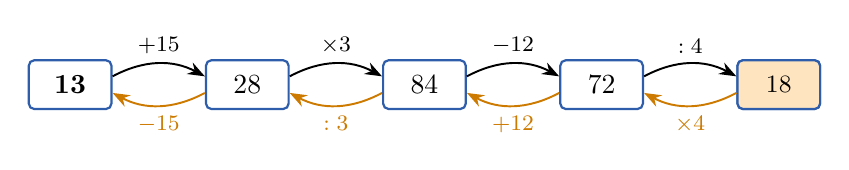
\begin{tikzpicture}[x=2.25cm,box/.style={draw=tmBlue!70!black,line width=0.8pt,rounded corners=2pt,minimum width=1.05cm,minimum height=0.62cm,font=\small}]
\foreach \v [count=\i from 0] in {?,28+15,84,72,18}{\node[box] (n\i) at (\i,0) {};}
\node at (n0) {$\mathbf{13}$}; \node at (n1) {$28$}; \node at (n2) {$84$}; \node at (n3) {$72$}; \node[box,fill=tmOrange!25] at (n4) {$18$};
\foreach \a/\b/\f/\g in {0/1/+15/-15,1/2/\times3/:3,2/3/-12/+12,3/4/:4/\times4}{
  \draw[-{Stealth},line width=0.7pt] ([yshift=3pt]n\a.east) to[bend left=28] node[above,font=\footnotesize]{$\f$} ([yshift=3pt]n\b.west);
  \draw[-{Stealth},line width=0.7pt,tmOrange!80!black] ([yshift=-3pt]n\b.west) to[bend left=28] node[below,font=\footnotesize]{$\g$} ([yshift=-3pt]n\a.east);}
\end{tikzpicture}
\end{center}
Backwards: $18\times4=72$;\par $72+12=84$;\par $84:3=28$;\par $28-15=13$.\par
\emph{Check:} $(13+15)\times3=84$;\par $84-12=72$;\par $72:4=18$.
\dapso{$13$.}
\end{exbox}
\gap
\begin{exbox}{\ExWord\ 2}
A woman takes eggs to market. First she sells half of them and $1$ more. Then she sells half of what is left and $1$ more. She has $10$ eggs left. How many did she bring?
\guide
\emph{Undo the second sale:} without the extra egg she would have $10+1=11$ left, which is half of what she had before.\par So before the second sale: $11\times2=22$ eggs.\par
\emph{Undo the first sale:} $(22+1)\times2=46$ eggs.
\dapso{$46$ eggs.}
\end{exbox}
\gap
\begin{exbox}{\ExWord\ 3}
On day one, $\dfrac13$ of the water in a tank is used; on day two, $\dfrac25$ of what is left. Now $120$ litres remain. How much water was in the tank at first?
\guide
After day two, $1-\dfrac25=\dfrac35$ of the day-one remainder is left.\par That remainder was $120:\dfrac35=200$ litres.\par
$200$ litres is $1-\dfrac13=\dfrac23$ of the original.\par At first: $200:\dfrac23=300$ litres.
\dapso{$300$ litres.}
\end{exbox}
\gap
\begin{exbox}{\ExWord\ 4}
Three drums hold $240$ litres of oil. First, drum I pours into drum II as much as drum II holds. Then drum II pours into drum III as much as drum III holds. Then drum III pours into drum I as much as drum I holds. Now all three drums hold the same. How much did each hold at first?
\guide
At the end each drum holds $240:3=80$ litres.\par A drum that ``receives as much as it holds'' doubles; going back, we \emph{halve} the receiving drum and \emph{give} that amount back to the pouring drum.
\begin{center}
\renewcommand{\arraystretch}{1.25}
\begin{tabular}{|l|c|c|c|}
\hline
 & Drum I & Drum II & Drum III\\\hline
At the end & $80$ & $80$ & $80$\\\hline
Before step 3 & $40$ & $80$ & $120$\\\hline
Before step 2 & $40$ & $140$ & $60$\\\hline
At first & $\mathbf{110}$ & $\mathbf{70}$ & $\mathbf{60}$\\\hline
\end{tabular}
\end{center}
\dapso{Drum I: $110$ litres; drum II: $70$ litres; drum III: $60$ litres.}
\end{exbox}
\dividerbar{Practice}
\begin{probbox}{1}{\relax}
Find a number such that multiplying it by $4$, subtracting $18$ and dividing by $2$ gives $25$.
\end{probbox}
\probsol{
$25\times2=50$;\par $50+18=68$;\par $68:4=17$.
\dapso{$17$.}}
\gap
\begin{probbox}{2}{\relax}
Nam thinks of a number. He multiplies it by $6$, adds $8$, divides by $2$ and subtracts $14$, getting $20$. What was his number?
\end{probbox}
\probsol{
$20+14=34$;\par $34\times2=68$;\par $68-8=60$;\par $60:6=10$.
\dapso{$10$.}}
\gap
\begin{probbox}{3}{\relax}
Find a number such that adding $\dfrac12$ and then multiplying by $\dfrac23$ gives $3$.
\end{probbox}
\probsol{
$3:\dfrac23=\dfrac92$;\par $\dfrac92-\dfrac12=4$.
\dapso{$4$.}}
\gap
\begin{probbox}{4}{\relax}
If An's age is doubled, $5$ is added and the result is divided by $3$, the answer is $9$. How old is An?
\end{probbox}
\probsol{
$9\times3=27$;\par $27-5=22$;\par $22:2=11$.
\dapso{$11$ years old.}}
\gap
\begin{probbox}{5}{\relax}
Lan spends $\dfrac12$ of her money on books and $\dfrac13$ of the rest on pens, leaving $20\,000$ dong. How much did she have at first?
\end{probbox}
\probsol{
$20\,000$ is $\dfrac23$ of what was left after the books, i.e.\par $30\,000$.\par At first: $30\,000\times2=60\,000$ dong.
\dapso{$60\,000$ dong.}}
\gap
\begin{probbox}{6}{\relax}
Hoa reads $\dfrac14$ of a book on day one, $\dfrac13$ of the remaining pages on day two, and the last $60$ pages on day three. How many pages does the book have?
\end{probbox}
\probsol{
$60$ pages are $\dfrac23$ of what was left after day one: $60:\dfrac23=90$.\par And $90$ pages are $\dfrac34$ of the book: $90:\dfrac34=120$.
\dapso{$120$ pages.}}
\gap
\begin{probbox}{7}{\relax}
Mr Ba sells half his hens and $2$ more, then half of the rest and $2$ more, and has $8$ left. How many hens did he have?
\end{probbox}
\probsol{
Before the second sale: $(8+2)\times2=20$.\par At first: $(20+2)\times2=44$.
\dapso{$44$ hens.}}
\gap
\begin{probbox}{8}{\relax}
At the market Mum first spends half her money and $5\,000$ dong more, then half the rest and $5\,000$ more, leaving $10\,000$ dong. How much did she take?
\end{probbox}
\probsol{
Before the second purchase: $(10\,000+5\,000)\times2=30\,000$.\par At first: $(30\,000+5\,000)\times2=70\,000$ dong.
\dapso{$70\,000$ dong.}}
\gap
\begin{probbox}{9}{\relax}
$15$ litres are poured from tank A into tank B, then $5$ litres from B back into A. Now each holds $40$ litres. How much did each hold at first?
\end{probbox}
\probsol{
Tank A: $40-5+15=50$ litres; tank B: $40+5-15=30$ litres.
\dapso{A: $50$ litres; B: $30$ litres.}}
\gap
\begin{probbox}{10}{\relax}
$6$ oranges move from basket I to basket II, then $2$ move from II back to I. Now basket I has $20$ and basket II has $30$. How many were in each at first?
\end{probbox}
\probsol{
Basket I: $20-2+6=24$; basket II: $30+2-6=26$.
\dapso{$24$ and $26$ oranges.}}
\gap
\begin{probbox}{11}{\relax}
Jar I pours half its water into jar II; then jar II pours $\dfrac13$ of what it holds into jar I. Now jar I has $8$ litres and jar II $12$. How much did each have at first?
\end{probbox}
\probsol{
Before the second pour, jar II kept $\dfrac23$, so it had $12:\dfrac23=18$ and gave $6$; jar I had $8-6=2$.\par
At first jar I had $2\times2=4$ and gave $2$; jar II had $18-2=16$.
\dapso{Jar I: $4$ litres; jar II: $16$ litres.}}
\gap
\begin{probbox}{12}{\relax}
Find a number: add $7$, multiply by $5$, then subtract $10$ to get $65$.
\end{probbox}
\probsol{
Before subtracting $10$: $65+10=75$.\par Before multiplying by $5$: $75:5=15$.\par Before adding $7$: $15-7=8$.
\dapso{$8$.}}
\gap
\begin{probbox}{13}{\relax}
Find a number: multiply by $3$, add $12$, then divide by $5$ to get $9$.
\end{probbox}
\probsol{
Before dividing by $5$: $9\times5=45$.\par Before adding $12$: $45-12=33$.\par The number: $33:3=11$.
\dapso{$11$.}}
\gap
\begin{probbox}{14}{\relax}
Find a number: subtract $4$, multiply by $6$, then add $3$ to get $51$.
\end{probbox}
\probsol{
Before adding $3$: $51-3=48$.\par Before multiplying by $6$: $48:6=8$.\par The number: $8+4=12$.
\dapso{$12$.}}
\gap
\begin{probbox}{15}{\relax}
Find a number: divide by $2$, add $15$, then multiply by $4$ to get $100$.
\end{probbox}
\probsol{
Before multiplying by $4$: $100:4=25$.\par Before adding $15$: $25-15=10$.\par The number: $10\times2=20$.
\dapso{$20$.}}
\gap
\begin{probbox}{16}{\relax}
Find $x$: multiply by $2.5$, then subtract $1.5$ to get $8.5$.
\end{probbox}
\probsol{
Before subtracting $1.5$: $8.5+1.5=10$.\par $x=10:2.5=4$.
\dapso{$x=4$.}}
\gap
\begin{probbox}{17}{\relax}
Find a decimal: add $2.4$, then multiply by $3$ to get $12.6$.
\end{probbox}
\probsol{
Before multiplying by $3$: $12.6:3=4.2$.\par The number: $4.2-2.4=1.8$.
\dapso{$1.8$.}}
\gap
\begin{probbox}{18}{\relax}
Mai spends $25\,000$ dong on a book, gets $10\,000$ dong from Mum, then spends $8\,000$ dong on a pen and has $17\,000$ dong left. How much did she start with?
\end{probbox}
\probsol{
Before the pen: $17\,000+8\,000=25\,000$ dong.\par Before Mum's gift: $25\,000-10\,000=15\,000$ dong.\par At first: $15\,000+25\,000=40\,000$ dong.
\dapso{$40\,000$ dong.}}
\gap
\begin{probbox}{19}{\relax}
A bus leaves the depot. At the first stop $6$ get off and $4$ get on; at the second $10$ get off and $3$ get on. Now $21$ passengers are aboard. How many were there at the start?
\end{probbox}
\probsol{
Before the second stop: $21-3+10=28$.\par Before the first stop: $28-4+6=30$.
\dapso{$30$ passengers.}}
\gap
\begin{probbox}{20}{\relax}
Dad's age divided by $4$, plus $3$, gives $13$. How old is Dad?
\end{probbox}
\probsol{
Before adding $3$: $13-3=10$.\par Dad's age: $10\times4=40$.
\dapso{$40$ years old.}}
\gap
\begin{probbox}{21}{\relax}
Lan spends $\dfrac13$ of her money, then $\dfrac12$ of the rest, and has $25\,000$ dong left. How much did she have?
\end{probbox}
\probsol{
$25\,000$ dong is $\dfrac12$ of what was left after the first spend.\par So $25\,000\times2=50\,000$ dong was left.\par That is $\dfrac23$ of the original.\par Original: $50\,000:\dfrac23=75\,000$ dong.
\dapso{$75\,000$ dong.}}
\gap
\begin{probbox}{22}{\relax}
On day one $\dfrac14$ of a tank's water is used; on day two $\dfrac13$ of the rest. $300$ litres remain. How much was there?
\end{probbox}
\probsol{
$300$ litres is $\dfrac23$ of what was left after day one.\par After day one: $300:\dfrac23=450$ litres.\par That is $\dfrac34$ of the original.\par Original: $450:\dfrac34=600$ litres.
\dapso{$600$ litres.}}
\gap
\begin{probbox}{23}{\relax}
A seller first sells half her eggs plus $2$, then half the rest plus $1$, leaving $9$. How many eggs were there?
\end{probbox}
\probsol{
Before the extra $1$: $9+1=10$, which is half of what was left after the first sale.\par After the first sale: $10\times2=20$.\par Likewise $20+2=22$ is half the original.\par Original: $22\times2=44$.
\dapso{$44$ eggs.}}
\gap
\begin{probbox}{24}{\relax}
Move $8$ pomelos from basket A to B, then $3$ from B to A. Now A has $25$ and B has $35$. How many did each have at first?
\end{probbox}
\probsol{
Before the second move: A $25-3=22$, B $35+3=38$.\par At first: A $22+8=30$, B $38-8=30$.
\dapso{$30$ in each.}}
\gap
\begin{probbox}{25}{\relax}
A shop sells $\dfrac25$ of its rice on day one and half the rest on day two, leaving $45$ kg. How much rice was there?
\end{probbox}
\probsol{
After day one: $45\times2=90$ kg.\par That is $\dfrac35$ of the original.\par Original: $90:\dfrac35=150$ kg.
\dapso{$150$ kg.}}
\gap
\begin{probbox}{26}{\relax}
Find $x$ if $\left(x-\dfrac13\right)\times\dfrac34=\dfrac12$.
\end{probbox}
\probsol{
$x-\dfrac13=\dfrac12:\dfrac34=\dfrac23$.\par $x=\dfrac23+\dfrac13=1$.
\dapso{$x=1$.}}
\gap
\begin{probbox}{27}{\relax}
An gives Binh $\dfrac13$ of his marbles, then gives Chi $4$, and has $12$ left. How many did An have?
\end{probbox}
\probsol{
Before giving Chi: $12+4=16$.\par That is $\dfrac23$ of the original.\par Original: $16:\dfrac23=24$.
\dapso{$24$ marbles.}}
\gap
\begin{probbox}{28}{\relax}
Find a number: multiply by $4$, add $0.6$, then divide by $2$ to get $5.3$.
\end{probbox}
\probsol{
Before dividing by $2$: $5.3\times2=10.6$.\par Before adding $0.6$: $10$.\par The number: $10:4=2.5$.
\dapso{$2.5$.}}
\gap
\begin{probbox}{29}{\relax}
From a roll of cloth, first $\dfrac14$ is cut, then $5$ m, then half of what remains, leaving $8$ m. How long was the roll?
\end{probbox}
\probsol{
Before the third cut: $8\times2=16$ m.\par Before the second: $16+5=21$ m.\par That is $\dfrac34$ of the roll.\par Roll: $21:\dfrac34=28$ m.
\dapso{$28$ m.}}
\gap
\begin{probbox}{30}{\relax}
Uncle Tu sells $\dfrac13$ of his ducks, then buys $15$ more and has $75$. How many ducks did he have?
\end{probbox}
\probsol{
Before buying: $75-15=60$.\par That is $\dfrac23$ of the flock.\par Original: $60:\dfrac23=90$.
\dapso{$90$ ducks.}}
\dividerbar{Challenge -- Extension}
\begin{probbox}{31}{\stars{1}}
A shop sells $\dfrac13$ of a roll of cloth and $2$ m more, then half of the rest and $3$ m more, leaving $12$ m. How long was the roll?
\end{probbox}
\probsol{
Before the second sale: $(12+3)\times2=30$ m.\par Then $30+2=32$ m is $\dfrac23$ of the roll, so the roll is $32:\dfrac23=48$ m.
\dapso{$48$ m.}}
\gap
\begin{probbox}{32}{\stars{1}}
A monkey picks some peaches. Each day it eats half of what it has and $1$ more. On the morning of day five it has just $1$ left. How many peaches did it pick?
\end{probbox}
\probsol{
The monkey ate for $4$ days.\par Undo each day with (number left $+1$)$\times2$.\par
$1\to4\to10\to22\to46$.
\dapso{$46$ peaches.}}
\gap
\begin{probbox}{33}{\stars{1}}
An, Binh and Cuong have $96$ marbles. An gives Binh as many as Binh has; then Binh gives Cuong as many as Cuong has; finally Cuong gives An as many as An has. Now they all have the same. How many did each have at first?
\end{probbox}
\probsol{
At the end each has $32$.\par Work backwards (as in Example $4$):\par
Before step 3: An $16$, Binh $32$, Cuong $48$.\par Before step 2: An $16$, Binh $56$, Cuong $24$.\par At first: An $44$, Binh $28$, Cuong $24$.
\dapso{An: $44$; Binh: $28$; Cuong: $24$ marbles.}}
\gap
\begin{probbox}{34}{\stars{2}}
A, B and C play three rounds of a game. After each round the loser must give each of the others as many marbles as they already have. A loses round 1, B round 2 and C round 3. Afterwards each has $24$ marbles. How many did each have at first?
\end{probbox}
\probsol{
Total: $72$ marbles.\par Going back, in each round the two winners halve and the loser gets those marbles back.\par
Before round 3: A $12$, B $12$, C $48$.\par Before round 2: A $6$, B $42$, C $24$.\par At first: A $39$, B $21$, C $12$.
\dapso{A: $39$; B: $21$; C: $12$ marbles.}}
\gap
\begin{probbox}{35}{\stars{1}}
Each day a monkey eats half its peaches plus $2$ more. After $3$ days it has $3$ left. How many did it start with?
\end{probbox}
\probsol{
Start of day three: $(3+2)\times2=10$.\par Start of day two: $(10+2)\times2=24$.\par At first: $(24+2)\times2=52$.
\dapso{$52$ peaches.}}
\gap
\begin{probbox}{36}{\stars{1}}
Pour from jar A into jar B as much as B holds; then from B into A as much as A holds. Now each has $24$ litres. How much did each have at first?
\end{probbox}
\probsol{
The second pour doubled A, so before it A had $24:2=12$ and B $24+12=36$.\par The first pour doubled B, so before it B had $36:2=18$ and A $12+18=30$.
\dapso{A $30$ litres, B $18$ litres.}}
\gap
\begin{probbox}{37}{\stars{1}}
A shop sells half its rice plus $5$ kg, then $\dfrac13$ of the rest plus $4$ kg, then $\dfrac14$ of the rest plus $3$ kg, leaving $15$ kg. How much was there?
\end{probbox}
\probsol{
Before the third sale: $15+3=18$ kg is $\dfrac34$, so $18:\dfrac34=24$ kg.\par Before the second: $24+4=28$ kg is $\dfrac23$, so $42$ kg.\par At first: $(42+5)\times2=94$ kg.
\dapso{$94$ kg.}}
\gap
\begin{probbox}{38}{\stars{1}}
Nam thinks of a number. Three times over he doubles it and subtracts $3$, ending with $19$. What was the number?
\end{probbox}
\probsol{
Before the third round: $(19+3):2=11$.\par Before the second: $(11+3):2=7$.\par The number: $(7+3):2=5$.
\dapso{$5$.}}
\gap
\begin{probbox}{39}{\stars{1}}
A team repairs a road: in week one $\dfrac14$ of it plus $3$ km; in week two $\dfrac13$ of the rest plus $1$ km; in week three the last $9$ km. How long is the road?
\end{probbox}
\probsol{
After week one, $9+1=10$ km is $\dfrac23$ of what was left, so $15$ km was left.\par $15+3=18$ km is $\dfrac34$ of the road.\par Road: $18:\dfrac34=24$ km.
\dapso{$24$ km.}}
\gap
\begin{probbox}{40}{\stars{1}}
Ms Hanh spends $\dfrac25$ of her pay on food, $\dfrac13$ of the rest on schooling and saves half of what remains, keeping $1\,200\,000$ dong. What is her pay?
\end{probbox}
\probsol{
Before saving: $1\,200\,000\times2=2\,400\,000$ dong.\par Before schooling: $2\,400\,000:\dfrac23=3\,600\,000$ dong.\par Pay: $3\,600\,000:\dfrac35=6\,000\,000$ dong.
\dapso{$6\,000\,000$ dong.}}
\gap
\begin{probbox}{41}{\stars{1}}
Grandpa's age minus $4$, divided by $7$, plus $2$, times $5$ is $60$. How old is he?
\end{probbox}
\probsol{
Before $\times5$: $12$.\par Before $+2$: $10$.\par Before $:7$: $70$.\par Age: $70+4=74$.
\dapso{$74$ years old.}}
\gap
\begin{probbox}{42}{\stars{1}}
Duckweed doubles its area every day and covers the whole pond at the end of day $10$. On which day did it cover $\dfrac14$ of the pond?
\end{probbox}
\probsol{
At the end of day $9$ it covered $\dfrac12$ (doubling gives the whole).\par At the end of day $8$ it covered $\dfrac14$.
\dapso{Day $8$.}}
\gap
\begin{probbox}{43}{\stars{1}}
Three drums hold $180$ litres. Pour $10$ l from I to II, then $20$ l from II to III, then $5$ l from III to I. Now all are equal. How much did each hold?
\end{probbox}
\probsol{
Finally each has $180:3=60$ l.\par Before the third pour: I $55$, III $65$.\par Before the second: II $80$, III $45$.\par At first: I $65$, II $70$, III $45$.
\dapso{I $65$ l, II $70$ l, III $45$ l.}}
\gap
\begin{probbox}{44}{\stars{1}}
Find $x$ if $(x\times1.5-2.25):0.5=7.5$.
\end{probbox}
\probsol{
$x\times1.5-2.25=7.5\times0.5=3.75$.\par $x\times1.5=6$.\par $x=4$.
\dapso{$x=4$.}}
\gap
\begin{probbox}{45}{\stars{1}}
Grandma spends half her money plus $3\,000$ dong, then half the rest plus $2\,000$, then half the rest plus $1\,000$, and has nothing left. How much did she take?
\end{probbox}
\probsol{
Before the third spend: $(0+1\,000)\times2=2\,000$ dong.\par Before the second: $(2\,000+2\,000)\times2=8\,000$ dong.\par At first: $(8\,000+3\,000)\times2=22\,000$ dong.
\dapso{$22\,000$ dong.}}
\gap
\begin{probbox}{46}{\stars{1}}
Two baskets hold $60$ oranges. Move $\dfrac13$ of basket I into II, then $\dfrac14$ of basket II (as it is then) into I. Now they are equal. How many were in each?
\end{probbox}
\probsol{
Finally each has $30$.\par Before the second move, II had $30:\dfrac34=40$, so I had $20$.\par Before the first, I had $20:\dfrac23=30$, so II had $30$.
\dapso{$30$ in each.}}
\gap
\begin{probbox}{47}{\stars{1}}
Ha does maths for $45$ minutes, rests $15$ minutes, then reads for $1$ hour $20$ minutes, finishing at $21{:}05$. When did she start?
\end{probbox}
\probsol{
Reading began at $21{:}05-1{:}20=19{:}45$.\par Rest began at $19{:}30$.\par Maths began at $18{:}45$.
\dapso{$18{:}45$.}}
\gap
\begin{probbox}{48}{\stars{1}}
Think of any number, multiply by $9$, add $18$, divide by $9$, then subtract the number you thought of. Show the result is always $2$.
\end{probbox}
\probsol{
Call the number $a$.\par $a\times9+18=(a+2)\times9$.\par Divide by $9$: $a+2$.\par Subtract $a$: $2$, whatever $a$ is.
\dapso{Always $2$.}}
\gap
\begin{probbox}{49}{\stars{2}}
A snail at the bottom of a $10$ m well climbs $3$ m each day and slips $2$ m each night. On which day does it reach the top?
\end{probbox}
\probsol{
Work back from the last day: it climbs $3$ m and reaches the top, so it started that day at $10-3=7$ m.\par Each day and night it gains $3-2=1$ m.\par Reaching $7$ m takes $7$ days and nights.\par So it gets out on day $8$.
\dapso{Day $8$.}}
\gap
\begin{probbox}{50}{\stars{2}}
Grandma has some apples. The eldest takes half plus half an apple; the second takes half the rest plus half an apple; the youngest takes half the rest plus half an apple, and none are left. No apple is cut. How many were there?
\end{probbox}
\probsol{
Before the youngest: $\left(0+\dfrac12\right)\times2=1$.\par Before the second: $\left(1+\dfrac12\right)\times2=3$.\par At first: $\left(3+\dfrac12\right)\times2=7$.\par Check: they take $4$, $2$ and $1$ whole apples.
\dapso{$7$ apples.}}
\clearpage
\titlehead
\begingroup\setbox0=\vbox{\section*{Triangles and Their Area}}\endgroup
\chapterhead{11}{Triangles and Their Area}

\shead{Base, height and area}
\begin{knowbox}
\begin{minipage}[t]{0.6\linewidth}
A \textbf{triangle} has $3$ sides, $3$ vertices and $3$ angles. By its angles it is \emph{acute} (three acute angles), \emph{obtuse} (one obtuse angle) or \emph{right-angled} (one right angle).\par
\smallskip
The segment drawn from a vertex \textbf{perpendicular} to the opposite side is a \textbf{height}; that side is the \textbf{base}. Every triangle has $3$ heights.\par
\smallskip
The \textbf{area of a triangle} is the base times the height (in the same unit), divided by $2$:
\[S=\frac{a\times h}{2}\qquad h=\frac{S\times2}{a}\qquad a=\frac{S\times2}{h}\]
In a right-angled triangle, the two sides at the right angle are each other's base and height.
\end{minipage}\hfill
\begin{minipage}[t]{0.36\linewidth}\vspace{2pt}
\centering
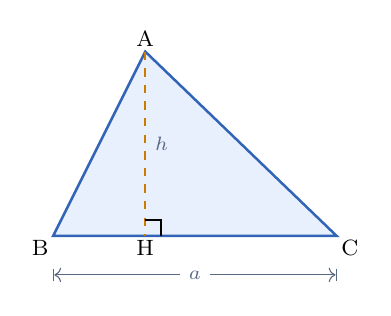
\begin{tikzpicture}[scale=0.9]
\coordinate (B) at (0,0); \coordinate (C) at (4,0); \coordinate (A) at (1.3,2.6); \coordinate (H) at (1.3,0);
\fill[tmBlue!12] (A)--(B)--(C)--cycle;
\draw[geo] (A)--(B)--(C)--cycle;
\draw[dashed,line width=0.7pt,tmOrange!80!black] (A)--(H);
\ramark{H}{C}{A}
\node[lbl,above] at (A){A}; \node[lbl,below left] at (B){B}; \node[lbl,below right] at (C){C}; \node[lbl,below] at (H){H};
\node[dim,right] at (1.3,1.3){$h$};
\draw[|<->|,Slate] (0,-0.55)--node[fill=white,dim]{$a$}(4,-0.55);
\end{tikzpicture}
\end{minipage}
\end{knowbox}
\gap
\begin{exbox}{\ExWord\ 1}
Find the area of a triangle with:
\begin{cols2}
\pa{a} base $8$ cm, height $5$ cm; & \pa{b} base $2.5$ dm, height $12$ cm.
\end{cols2}
\guide
\pa{a} $S=8\times5:2=20$ cm$^2$.\par
\pa{b} Use the same unit first: $2.5$ dm $=25$ cm.\par $S=25\times12:2=150$ cm$^2$.
\dapso{\pa{a} $20$ cm$^2$;\par \pa{b} $150$ cm$^2$.}
\end{exbox}
\gap
\begin{exbox}{\ExWord\ 2}
\begin{minipage}[t]{0.62\linewidth}
Triangle ABC has a right angle at A, with $AB=6$ cm, $AC=8$ cm and $BC=10$ cm. Find its area and the length of the height AH.
\end{minipage}\hfill
\begin{minipage}[t]{0.34\linewidth}\vspace{0pt}\centering
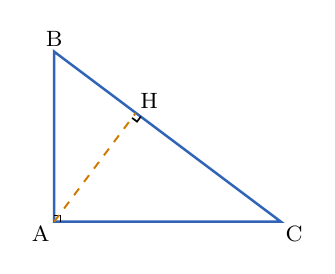
\begin{tikzpicture}[scale=0.36]
\coordinate (A) at (0,0); \coordinate (B) at (0,6); \coordinate (C) at (8,0); \coordinate (H) at (2.88,3.84);
\draw[geo] (A)--(B)--(C)--cycle; \ramark{A}{B}{C}
\draw[dashed,line width=0.7pt,tmOrange!80!black] (A)--(H); \ramark{H}{C}{A}
\node[lbl,below left] at (A){A}; \node[lbl,above] at (B){B}; \node[lbl,below right] at (C){C}; \node[lbl,above right] at (H){H};
\end{tikzpicture}
\end{minipage}
\guide
Take AC as the base; then AB is the height: $S=6\times8:2=24$ cm$^2$.\par
Take BC as the base; then AH is the height: $AH=24\times2:10=4.8$ cm.
\dapso{$24$ cm$^2$;\par $AH=4.8$ cm.}
\end{exbox}
\gap
\begin{exbox}{\ExWord\ 3}
A triangle has area $36$ cm$^2$ and base $9$ cm. Find its height.
\guide
$h=S\times2:a=36\times2:9=8$ cm.
\dapso{$8$ cm.}
\end{exbox}
\gap
\begin{exbox}{\ExWord\ 4}
\begin{minipage}[t]{0.6\linewidth}
Rectangle ABCD has $AB=12$ cm and $BC=8$ cm; M is the midpoint of BC. Find the areas of triangles ABM, MCD and AMD.
\end{minipage}\hfill
\begin{minipage}[t]{0.36\linewidth}\vspace{0pt}\centering
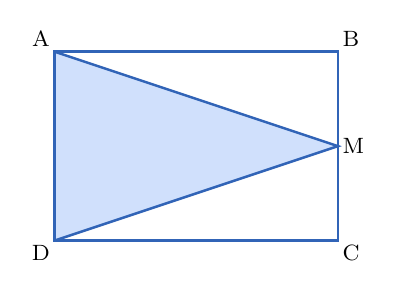
\begin{tikzpicture}[scale=0.3]
\coordinate (A) at (0,8); \coordinate (B) at (12,8); \coordinate (C) at (12,0); \coordinate (D) at (0,0); \coordinate (M) at (12,4);
\fill[shade] (A)--(M)--(D)--cycle;
\draw[geo] (A)--(B)--(C)--(D)--cycle; \draw[geo] (A)--(M)--(D);
\node[lbl,above left] at (A){A}; \node[lbl,above right] at (B){B}; \node[lbl,below right] at (C){C}; \node[lbl,below left] at (D){D}; \node[lbl,right] at (M){M};
\end{tikzpicture}
\end{minipage}
\guide
$BM=MC=8:2=4$ cm.\par $S_{ABM}=12\times4:2=24$ cm$^2$;\par $S_{MCD}=12\times4:2=24$ cm$^2$.\par
$S_{ABCD}=12\times8=96$ cm$^2$, so $S_{AMD}=96-24-24=48$ cm$^2$.\par
\emph{Remark:} triangle AMD has base AD and height equal to AB, so its area is half the rectangle.
\dapso{$24$ cm$^2$; $24$ cm$^2$; $48$ cm$^2$.}
\end{exbox}
\dividerbar{Practice}
\begin{probbox}{1}{\relax}
Find the area of a triangle with base $a$ and height $h$:
\begin{cols2}
\pa{a} $a=15$ cm, $h=8$ cm; & \pa{b} $a=4.5$ m, $h=2$ m;\\
\pa{c} $a=\dfrac34$ m, $h=\dfrac25$ m; & \pa{d} $a=1.2$ dm, $h=15$ cm.
\end{cols2}
\end{probbox}
\probsol{
\pa{a} $15\times8:2=60$ cm$^2$.\par \pa{b} $4.5\times2:2=4.5$ m$^2$.\par \pa{c} $\dfrac34\times\dfrac25:2=\dfrac3{20}$ m$^2$.\par \pa{d} $1.2$ dm $=12$ cm; $12\times15:2=90$ cm$^2$.
\dapso{$60$ cm$^2$; $4.5$ m$^2$; $\dfrac3{20}$ m$^2$; $90$ cm$^2$.}}
\gap
\begin{probbox}{2}{\relax}
Find the area of a right-angled triangle whose two shorter sides are $3.5$ dm and $2$ dm.
\end{probbox}
\probsol{
$S=3.5\times2:2=3.5$ dm$^2$.
\dapso{$3.5$ dm$^2$.}}
\gap
\begin{probbox}{3}{\relax}
A triangle has area $45$ cm$^2$ and height $6$ cm. Find its base.
\end{probbox}
\probsol{
$a=45\times2:6=15$ cm.
\dapso{$15$ cm.}}
\gap
\begin{probbox}{4}{\relax}
A triangular plot has base $40$ m and height $\dfrac34$ of the base. Find its area.
\end{probbox}
\probsol{
Height: $40\times\dfrac34=30$ m.\par Area: $40\times30:2=600$ m$^2$.
\dapso{$600$ m$^2$.}}
\gap
\begin{probbox}{5}{\relax}
A triangular card has base $2.4$ dm and height $\dfrac23$ of the base. Find its area.
\end{probbox}
\probsol{
Height: $2.4\times\dfrac23=1.6$ dm.\par Area: $2.4\times1.6:2=1.92$ dm$^2$.
\dapso{$1.92$ dm$^2$.}}
\gap
\begin{probbox}{6}{\relax}
Triangle ABC has a right angle at A, $AB=9$ cm, $AC=12$ cm and $BC=15$ cm. Find the height AH.
\end{probbox}
\probsol{
$S=9\times12:2=54$ cm$^2$.\par $AH=54\times2:15=7.2$ cm.
\dapso{$7.2$ cm.}}
\gap
\begin{probbox}{7}{\relax}
A triangle has the same area as a square of side $6$ cm. Its base is $9$ cm. Find its height.
\end{probbox}
\probsol{
Area: $6\times6=36$ cm$^2$.\par Height: $36\times2:9=8$ cm.
\dapso{$8$ cm.}}
\gap
\begin{probbox}{8}{\relax}
A triangle has base $18$ cm. Lengthening the base by $4$ cm (same height) adds $20$ cm$^2$ to the area. Find the original area.
\end{probbox}
\probsol{
The extra part is a triangle with base $4$ cm and area $20$ cm$^2$; its height is $20\times2:4=10$ cm.\par
Original area: $18\times10:2=90$ cm$^2$.
\dapso{$90$ cm$^2$.}}
\gap
\begin{probbox}{9}{\relax}
Square ABCD has side $10$ cm; M is the midpoint of BC. Find the areas of triangle ABM and quadrilateral AMCD.
\end{probbox}
\probsol{
$S_{ABM}=10\times5:2=25$ cm$^2$.\par $S_{AMCD}=10\times10-25=75$ cm$^2$.
\dapso{$25$ cm$^2$; $75$ cm$^2$.}}
\gap
\begin{probbox}{10}{\relax}
Triangle ABC has area $60$ cm$^2$ and $BC=15$ cm. Point M lies on BC with $BM=5$ cm. Find the area of triangle ABM.
\end{probbox}
\probsol{
The height from A to BC is $60\times2:15=8$ cm.\par Triangle ABM has the same height: $S_{ABM}=5\times8:2=20$ cm$^2$.
\dapso{$20$ cm$^2$.}}
\gap
\begin{probbox}{11}{\relax}
\begin{minipage}[t]{0.62\linewidth}
How many triangles are there in the figure? Name them.
\end{minipage}\hfill
\begin{minipage}[t]{0.34\linewidth}\vspace{0pt}\centering
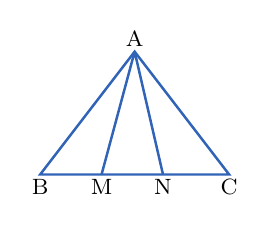
\begin{tikzpicture}[scale=0.6]
\coordinate (A) at (2,2.6); \coordinate (B) at (0,0); \coordinate (M) at (1.3,0); \coordinate (N) at (2.6,0); \coordinate (C) at (4,0);
\draw[geo] (A)--(B)--(C)--cycle; \draw[geo] (A)--(M) (A)--(N);
\node[lbl,above] at (A){A}; \node[lbl,below] at (B){B}; \node[lbl,below] at (M){M}; \node[lbl,below] at (N){N}; \node[lbl,below] at (C){C};
\end{tikzpicture}
\end{minipage}
\end{probbox}
\probsol{
Each triangle has vertex A and a base joining two of the four points B, M, N, C.\par There are $3+2+1=6$ such segments.\par
Triangles: ABM, AMN, ANC, ABN, AMC, ABC.
\dapso{$6$ triangles.}}
\gap
\begin{probbox}{12}{\relax}
Find the area of a triangle with base $14$ cm and height $9$ cm.
\end{probbox}
\probsol{
$S=14\times9:2=63$ cm$^2$.
\dapso{$63$ cm$^2$.}}
\gap
\begin{probbox}{13}{\relax}
Find the area of a triangle with base $2.5$ m and height $1.6$ m.
\end{probbox}
\probsol{
$S=2.5\times1.6:2=2$ m$^2$.
\dapso{$2$ m$^2$.}}
\gap
\begin{probbox}{14}{\relax}
Find the area of a triangle with base $\dfrac34$ m and height $\dfrac25$ m.
\end{probbox}
\probsol{
$S=\dfrac34\times\dfrac25:2=\dfrac3{20}$ m$^2$.
\dapso{$\dfrac3{20}$ m$^2$.}}
\gap
\begin{probbox}{15}{\relax}
Find the area of a triangle with base $3$ dm and height $25$ cm.
\end{probbox}
\probsol{
$3$ dm $=30$ cm.\par $S=30\times25:2=375$ cm$^2$.
\dapso{$375$ cm$^2$.}}
\gap
\begin{probbox}{16}{\relax}
Find the area of a right triangle whose legs are $7$ cm and $10$ cm.
\end{probbox}
\probsol{
One leg is the base and the other the height.\par $S=7\times10:2=35$ cm$^2$.
\dapso{$35$ cm$^2$.}}
\gap
\begin{probbox}{17}{\relax}
A triangle has area $54$ cm$^2$ and base $12$ cm. Find its height.
\end{probbox}
\probsol{
Height $=$ area $\times2\,:$ base.\par $h=54\times2:12=9$ cm.
\dapso{$9$ cm.}}
\gap
\begin{probbox}{18}{\relax}
A triangle has area $7.5$ dm$^2$ and height $2.5$ dm. Find its base.
\end{probbox}
\probsol{
Base $=$ area $\times2\,:$ height.\par $a=7.5\times2:2.5=6$ dm.
\dapso{$6$ dm.}}
\gap
\begin{probbox}{19}{\relax}
A triangular plot has base $50$ m and height $24$ m. Each square metre yields $0.8$ kg of vegetables. What is the total yield?
\end{probbox}
\probsol{
Area: $50\times24:2=600$ m$^2$.\par Yield: $0.8\times600=480$ kg.
\dapso{$480$ kg.}}
\gap
\begin{probbox}{20}{\relax}
A triangle has base $16$ cm and height $\dfrac34$ of the base. Find its area.
\end{probbox}
\probsol{
Height: $16\times\dfrac34=12$ cm.\par Area: $16\times12:2=96$ cm$^2$.
\dapso{$96$ cm$^2$.}}
\gap
\begin{probbox}{21}{\relax}
The base and height of a triangle add up to $30$ cm, and the base is $6$ cm longer. Find the area.
\end{probbox}
\probsol{
Base: $(30+6):2=18$ cm.\par Height: $12$ cm.\par Area: $18\times12:2=108$ cm$^2$.
\dapso{$108$ cm$^2$.}}
\gap
\begin{probbox}{22}{\relax}
Triangle ABC has a right angle at A, $AB=15$ cm, $AC=20$ cm, $BC=25$ cm. Find its area and the height AH.
\end{probbox}
\probsol{
Area: $15\times20:2=150$ cm$^2$.\par With BC as base, AH is the height.\par $AH=150\times2:25=12$ cm.
\dapso{$150$ cm$^2$; $AH=12$ cm.}}
\gap
\begin{probbox}{23}{\relax}
Triangle one has base $12$ cm and height $8$ cm. Triangle two has the same area and base $16$ cm. Find its height.
\end{probbox}
\probsol{
Area: $12\times8:2=48$ cm$^2$.\par Height of triangle two: $48\times2:16=6$ cm.
\dapso{$6$ cm.}}
\gap
\begin{probbox}{24}{\relax}
Each triangular flag has base $30$ cm and height $20$ cm. How many square decimetres of cloth do $20$ flags need? (Ignore seams.)
\end{probbox}
\probsol{
One flag: $30\times20:2=300$ cm$^2$.\par $20$ flags: $6\,000$ cm$^2$ $=60$ dm$^2$.
\dapso{$60$ dm$^2$.}}
\gap
\begin{probbox}{25}{\relax}
A right triangle has area $24$ cm$^2$ and one leg $6$ cm. Find the other leg.
\end{probbox}
\probsol{
The other leg is the height for the base $6$ cm.\par Length: $24\times2:6=8$ cm.
\dapso{$8$ cm.}}
\gap
\begin{probbox}{26}{\relax}
Rectangle ABCD is $12$ cm by $8$ cm. Diagonal AC cuts it into two triangles. Find the area of each.
\end{probbox}
\probsol{
Triangle ABC has a right angle at B with legs $12$ cm and $8$ cm.\par $S_{ABC}=12\times8:2=48$ cm$^2$.\par Likewise $S_{ACD}=48$ cm$^2$ (half the rectangle).
\dapso{$48$ cm$^2$ each.}}
\gap
\begin{probbox}{27}{\relax}
A triangle has area $150$ cm$^2$. Raising its height by $3$ cm (same base) adds $30$ cm$^2$. Find the base and the height.
\end{probbox}
\probsol{
The extra part is a triangle with the same base, height $3$ cm and area $30$ cm$^2$.\par Base: $30\times2:3=20$ cm.\par Height: $150\times2:20=15$ cm.
\dapso{Base $20$ cm, height $15$ cm.}}
\gap
\begin{probbox}{28}{\relax}
A triangle with base $8$ cm has the same area as a square of side $8$ cm. Find its height.
\end{probbox}
\probsol{
Square: $8\times8=64$ cm$^2$.\par Height: $64\times2:8=16$ cm.
\dapso{$16$ cm.}}
\gap
\begin{probbox}{29}{\relax}
A triangular field has base $120$ m and height $80$ m. Give its area in hectares.
\end{probbox}
\probsol{
Area: $120\times80:2=4\,800$ m$^2$.\par $1$ ha $=10\,000$ m$^2$, so this is $0.48$ ha.
\dapso{$0.48$ ha.}}
\gap
\begin{probbox}{30}{\relax}
Triangle ABC has area $48$ cm$^2$; M is the midpoint of BC. Find the area of triangle ABM.
\end{probbox}
\probsol{
ABM and ABC share the height from A.\par $BM=\dfrac12BC$, so $S_{ABM}=\dfrac12S_{ABC}$.\par $S_{ABM}=48:2=24$ cm$^2$.
\dapso{$24$ cm$^2$.}}
\dividerbar{Challenge -- Extension}
\begin{probbox}{31}{\stars{1}}
A triangle has area $120$ cm$^2$. Shortening the base by $3$ cm (same height) takes $18$ cm$^2$ off the area. Find the base.
\end{probbox}
\probsol{
Height: $18\times2:3=12$ cm.\par Base: $120\times2:12=20$ cm.
\dapso{$20$ cm.}}
\gap
\begin{probbox}{32}{\stars{1}}
The two shorter sides of a right-angled triangle add up to $14$ cm, and one is $2$ cm longer than the other. Find its area.
\end{probbox}
\probsol{
The sides are $(14+2):2=8$ cm and $6$ cm.\par Area: $8\times6:2=24$ cm$^2$.
\dapso{$24$ cm$^2$.}}
\gap
\begin{probbox}{33}{\stars{1}}
Rectangle ABCD has $AB=16$ cm and $AD=10$ cm. Point E is on AB with $AE=6$ cm. Find the areas of triangles ADE, EBC and ECD.
\end{probbox}
\probsol{
$S_{ADE}=6\times10:2=30$ cm$^2$;\par $EB=10$ cm, so $S_{EBC}=10\times10:2=50$ cm$^2$.\par
$S_{ECD}=16\times10:2=80$ cm$^2$ (half the rectangle).\par \emph{Check:} $30+50+80=160=16\times10$.
\dapso{$30$ cm$^2$; $50$ cm$^2$; $80$ cm$^2$.}}
\gap
\begin{probbox}{34}{\stars{2}}
Triangle ABC has a right angle at A, $AB=6$ cm and $AC=8$ cm. M is on AB with $AM=2$ cm, and N is on AC with $AN=4$ cm. Find the area of quadrilateral BMNC.
\end{probbox}
\probsol{
$S_{ABC}=6\times8:2=24$ cm$^2$;\par $S_{AMN}=2\times4:2=4$ cm$^2$.\par $S_{BMNC}=24-4=20$ cm$^2$.
\dapso{$20$ cm$^2$.}}
\gap
\begin{probbox}{35}{\stars{2}}
\begin{minipage}[t]{0.62\linewidth}
How many triangles are there in the figure?
\end{minipage}\hfill
\begin{minipage}[t]{0.34\linewidth}\vspace{0pt}\centering
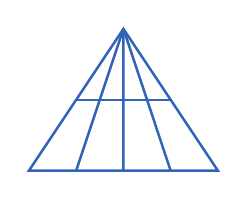
\begin{tikzpicture}[scale=0.6]
\coordinate (A) at (2,3); \coordinate (B) at (0,0); \coordinate (C) at (4,0);
\draw[geo] (A)--(B)--(C)--cycle;
\foreach \x in {1,2,3}{\draw[geo] (A)--(\x,0);}
\draw[geo] (1,1.5)--(3,1.5);
\end{tikzpicture}
\end{minipage}
\end{probbox}
\probsol{
Ignoring the middle crossbar: the base has $5$ points, giving $4+3+2+1=10$ triangles with vertex A.\par
The crossbar also has $5$ points, giving $10$ more triangles with vertex A.\par In all: $20$ triangles.
\dapso{$20$ triangles.}}
\gap
\begin{probbox}{36}{\stars{1}}
In triangle ABC, $BC=20$ cm. M lies on BC with $BM=8$ cm, and triangle ABM has area $40$ cm$^2$. Find the area of ABC.
\end{probbox}
\probsol{
The common height from A: $40\times2:8=10$ cm.\par $S_{ABC}=20\times10:2=100$ cm$^2$.
\dapso{$100$ cm$^2$.}}
\gap
\begin{probbox}{37}{\stars{1}}
Rectangle ABCD has $AB=20$ cm, $AD=12$ cm. M is the midpoint of AB and N the midpoint of BC. Find the area of triangle DMN.
\end{probbox}
\probsol{
Rectangle: $20\times12=240$ cm$^2$.\par $S_{AMD}=60$, $S_{MBN}=30$, $S_{NCD}=60$ cm$^2$.\par $S_{DMN}=240-60-30-60=90$ cm$^2$.
\dapso{$90$ cm$^2$.}}
\gap
\begin{probbox}{38}{\stars{1}}
Square ABCD has side $12$ cm, and E is any point on AB. Find the area of triangle ECD and the total area of triangles AED and EBC.
\end{probbox}
\probsol{
Triangle ECD has base $CD=12$ cm and height $12$ cm.\par $S_{ECD}=72$ cm$^2$.\par The other two total $144-72=72$ cm$^2$, wherever E is.
\dapso{Both are $72$ cm$^2$.}}
\gap
\begin{probbox}{39}{\stars{1}}
A triangle has area $40$ cm$^2$. If its base is tripled and its height halved, what is the new area?
\end{probbox}
\probsol{
Tripling the base triples the area.\par Halving the height halves it.\par New area: $40\times3:2=60$ cm$^2$.
\dapso{$60$ cm$^2$.}}
\gap
\begin{probbox}{40}{\stars{1}}
The legs of a right triangle add up to $23$ cm and differ by $7$ cm. Find its area.
\end{probbox}
\probsol{
Longer leg: $(23+7):2=15$ cm.\par Shorter: $8$ cm.\par Area: $15\times8:2=60$ cm$^2$.
\dapso{$60$ cm$^2$.}}
\gap
\begin{probbox}{41}{\stars{1}}
Triangle ABC has area $90$ cm$^2$. M on BC makes $MC$ twice $BM$. Find the areas of ABM and AMC.
\end{probbox}
\probsol{
$BM=\dfrac13BC$ and $MC=\dfrac23BC$; both share the height from A.\par $S_{ABM}=90:3=30$ cm$^2$.\par $S_{AMC}=60$ cm$^2$.
\dapso{$S_{ABM}=30$ cm$^2$, $S_{AMC}=60$ cm$^2$.}}
\gap
\begin{probbox}{42}{\stars{1}}
Triangle ABC has a right angle at A, $AB=12$ cm, $AC=16$ cm. M is the midpoint of AC. Compare the areas of ABM and BMC.
\end{probbox}
\probsol{
$AM=MC=8$ cm; both have height $AB=12$ cm.\par $S_{ABM}=48$ cm$^2$.\par $S_{BMC}=48$ cm$^2$.\par They are equal.
\dapso{Equal, $48$ cm$^2$ each.}}
\gap
\begin{probbox}{43}{\stars{1}}
Triangle ABC has $BC=24$ cm and height $AH=10$ cm. BC is extended beyond C by $CD=6$ cm. Find the areas of ACD and ABD.
\end{probbox}
\probsol{
ABC, ACD and ABD all have height $AH=10$ cm.\par $S_{ACD}=6\times10:2=30$ cm$^2$.\par $S_{ABD}=30\times10:2=150$ cm$^2$.
\dapso{$30$ cm$^2$ and $150$ cm$^2$.}}
\gap
\begin{probbox}{44}{\stars{1}}
Two triangles have equal heights. The base of the first is $\dfrac23$ of the second's, and the second's area is $24$ cm$^2$ larger. Find each area.
\end{probbox}
\probsol{
With equal heights, areas are in the ratio of the bases: $S_1=\dfrac23S_2$.\par The difference of $3-2=1$ part is $24$ cm$^2$.\par $S_1=48$ cm$^2$; $S_2=72$ cm$^2$.
\dapso{$48$ cm$^2$ and $72$ cm$^2$.}}
\gap
\begin{probbox}{45}{\stars{1}}
A garden is $40$ m by $25$ m. Flowers grow on a triangle whose base is one long side and whose apex is on the opposite side; grass covers the rest. Find both areas.
\end{probbox}
\probsol{
The triangle has base $40$ m and height $25$ m.\par Flowers: $500$ m$^2$.\par Garden: $1\,000$ m$^2$.\par Grass: $500$ m$^2$.
\dapso{Flowers $500$ m$^2$, grass $500$ m$^2$.}}
\gap
\begin{probbox}{46}{\stars{1}}
Triangle ABC has area $72$ cm$^2$. D is on AB with $AD=\dfrac13AB$; E is the midpoint of AC. Find the area of ADE.
\end{probbox}
\probsol{
Join D to C.\par ADC and ABC share the height from C, and $AD=\dfrac13AB$.\par $S_{ADC}=72:3=24$ cm$^2$.\par ADE and ADC share the height from D, and $AE=\dfrac12AC$.\par $S_{ADE}=12$ cm$^2$.
\dapso{$12$ cm$^2$.}}
\gap
\begin{probbox}{47}{\stars{1}}
Square ABCD has side $10$ cm. E is the midpoint of BC and F the midpoint of CD. Find the area of triangle AEF.
\end{probbox}
\probsol{
$S_{ABE}=25$ cm$^2$; $S_{ADF}=25$ cm$^2$.\par $S_{ECF}=5\times5:2=12.5$ cm$^2$.\par $S_{AEF}=100-25-25-12.5=37.5$ cm$^2$.
\dapso{$37.5$ cm$^2$.}}
\gap
\begin{probbox}{48}{\stars{2}}
A square has a diagonal of $8$ cm. Find its area.
\end{probbox}
\probsol{
A diagonal splits the square into two equal triangles on the base $8$ cm.\par The diagonals are equal, perpendicular and bisect each other, so each triangle's height is $8:2=4$ cm.\par Each triangle: $8\times4:2=16$ cm$^2$.\par Square: $32$ cm$^2$.
\dapso{$32$ cm$^2$.}}
\gap
\begin{probbox}{49}{\stars{2}}
Triangle ABC has area $80$ cm$^2$. M is the midpoint of BC and N the midpoint of AM. Find the area of BNC.
\end{probbox}
\probsol{
$S_{ABM}=S_{ACM}=40$ cm$^2$.\par BNM and BAM share the height from B and $NM=\dfrac12AM$, so $S_{BNM}=20$ cm$^2$.\par Likewise $S_{CNM}=20$ cm$^2$.\par $S_{BNC}=40$ cm$^2$.
\dapso{$40$ cm$^2$.}}
\gap
\begin{probbox}{50}{\stars{2}}
Triangle ABC has area $120$ cm$^2$. M is on BC with $BM=\dfrac14BC$; N is on AM with $AN=\dfrac23AM$. Find the areas of ABN and NBM.
\end{probbox}
\probsol{
$S_{ABM}=120:4=30$ cm$^2$ (same height from A).\par ABN and ABM share the height from B, with $AN=\dfrac23AM$.\par $S_{ABN}=20$ cm$^2$.\par $S_{NBM}=10$ cm$^2$.
\dapso{$S_{ABN}=20$ cm$^2$, $S_{NBM}=10$ cm$^2$.}}
\clearpage
\titlehead
\begingroup\setbox0=\vbox{\section*{(*) Comparing Areas of Triangles}}\endgroup
\chapterhead{12}{(*) Comparing Areas of Triangles}

\shead{Same height, compare the bases}
\begin{knowbox}
\begin{minipage}[t]{0.6\linewidth}
\begin{itemize}[leftmargin=1.4em,itemsep=3pt]
\item Two triangles with \textbf{the same height} have areas in the same ratio as \textbf{their bases}. For example, if M is on BC then
\[\frac{S_{ABM}}{S_{AMC}}=\frac{BM}{MC}.\]
\item Two triangles with \textbf{the same base} have areas in the same ratio as \textbf{their heights}.
\item The segment from a vertex to the \textbf{midpoint} of the opposite side splits a triangle into two triangles of equal area.
\end{itemize}
To compare two triangles, it often helps to pass through a ``middle'' triangle that shares a height with each of them.
\end{minipage}\hfill
\begin{minipage}[t]{0.36\linewidth}\vspace{4pt}\centering
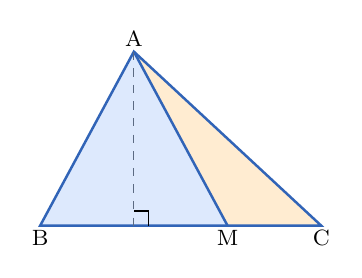
\begin{tikzpicture}[scale=0.85]
\coordinate (B) at (0,0); \coordinate (C) at (4.2,0); \coordinate (A) at (1.4,2.6); \coordinate (M) at (2.8,0); \coordinate (H) at (1.4,0);
\fill[tmBlue!18] (A)--(B)--(M)--cycle; \fill[tmOrange!18] (A)--(M)--(C)--cycle;
\draw[geo] (A)--(B)--(C)--cycle; \draw[geo] (A)--(M);
\draw[dashed,Slate] (A)--(H); \ramark{H}{C}{A}
\node[lbl,above] at (A){A}; \node[lbl,below] at (B){B}; \node[lbl,below] at (C){C}; \node[lbl,below] at (M){M};
\end{tikzpicture}
\end{minipage}
\end{knowbox}
\gap
\begin{exbox}{\ExWord\ 1}
Triangle ABC has area $45$ cm$^2$. Point M is on BC with $BM$ twice $MC$. Find the areas of triangles ABM and AMC.
\guide
Triangles ABM and AMC share the height from A, so their areas are in the ratio $BM:MC=2:1$.\par If $S_{AMC}$ is $1$ part, $S_{ABM}$ is $2$ parts and $S_{ABC}$ is $3$ parts.\par
$S_{AMC}=45:3=15$ cm$^2$;\par $S_{ABM}=15\times2=30$ cm$^2$.
\dapso{$30$ cm$^2$ and $15$ cm$^2$.}
\end{exbox}
\gap
\begin{exbox}{\ExWord\ 2}
\begin{minipage}[t]{0.6\linewidth}
Triangle ABC has area $60$ cm$^2$; M is the midpoint of BC and N is the midpoint of AM. Find the areas of triangles ABN and BNC.
\end{minipage}\hfill
\begin{minipage}[t]{0.36\linewidth}\vspace{0pt}\centering
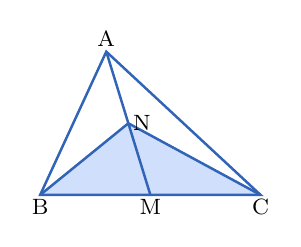
\begin{tikzpicture}[scale=0.7]
\coordinate (B) at (0,0); \coordinate (C) at (4,0); \coordinate (A) at (1.2,2.6); \coordinate (M) at (2,0); \coordinate (N) at (1.6,1.3);
\fill[shade] (B)--(N)--(C)--cycle;
\draw[geo] (A)--(B)--(C)--cycle; \draw[geo] (A)--(M) (B)--(N)--(C);
\node[lbl,above] at (A){A}; \node[lbl,below] at (B){B}; \node[lbl,below] at (C){C}; \node[lbl,below] at (M){M}; \node[lbl,right] at (N){N};
\end{tikzpicture}
\end{minipage}
\guide
M is the midpoint of BC, so $S_{ABM}=S_{AMC}=60:2=30$ cm$^2$.\par
N is the midpoint of AM, so $S_{ABN}=S_{NBM}=30:2=15$ cm$^2$; likewise $S_{NMC}=15$ cm$^2$.\par
$S_{BNC}=S_{NBM}+S_{NMC}=15+15=30$ cm$^2$.
\dapso{$S_{ABN}=15$ cm$^2$;\par $S_{BNC}=30$ cm$^2$.}
\end{exbox}
\gap
\begin{exbox}{\ExWord\ 3}
Triangle ABC has area $72$ cm$^2$. M is on AB with $AM=\dfrac13AB$, and N is on AC with $AN=\dfrac12AC$. Find the areas of triangle AMN and quadrilateral BMNC.
\guide
Join M to C (the ``middle'' triangle AMC).\par
AMC and ABC share the height from C, and $AM=\dfrac13AB$, so $S_{AMC}=\dfrac13\times72=24$ cm$^2$.\par
AMN and AMC share the height from M, and $AN=\dfrac12AC$, so $S_{AMN}=\dfrac12\times24=12$ cm$^2$.\par
$S_{BMNC}=72-12=60$ cm$^2$.
\dapso{$12$ cm$^2$; $60$ cm$^2$.}
\end{exbox}
\gap
\begin{exbox}{\ExWord\ 4}
Square ABCD has side $12$ cm; M is the midpoint of AB and N the midpoint of BC. Find the area of triangle DMN.
\guide
Take the square and remove the three right-angled corner triangles:\par
$S_{AMD}=6\times12:2=36$;\par $S_{MBN}=6\times6:2=18$;\par $S_{NCD}=6\times12:2=36$ cm$^2$.\par
$S_{DMN}=12\times12-36-18-36=54$ cm$^2$.
\dapso{$54$ cm$^2$.}
\end{exbox}
\dividerbar{Practice}
\begin{probbox}{1}{\relax}
Triangle ABC has area $40$ cm$^2$. M is on BC with $BM=3$ cm and $MC=5$ cm. Find the areas of ABM and AMC.
\end{probbox}
\probsol{
The areas are in the ratio $3:5$, $8$ parts in all.\par $S_{ABM}=40:8\times3=15$ cm$^2$; $S_{AMC}=25$ cm$^2$.
\dapso{$15$ cm$^2$ and $25$ cm$^2$.}}
\gap
\begin{probbox}{2}{\relax}
In triangle ABC, M is the midpoint of BC and $S_{ABM}=18$ cm$^2$. Find $S_{ABC}$.
\end{probbox}
\probsol{
$S_{AMC}=S_{ABM}=18$ cm$^2$, so $S_{ABC}=36$ cm$^2$.
\dapso{$36$ cm$^2$.}}
\gap
\begin{probbox}{3}{\relax}
Triangle ABC has area $90$ cm$^2$. D is on AC with $AD=\dfrac23AC$. Find the areas of ABD and BDC.
\end{probbox}
\probsol{
They share the height from B: $S_{ABD}=\dfrac23\times90=60$ cm$^2$ and $S_{BDC}=30$ cm$^2$.
\dapso{$60$ cm$^2$ and $30$ cm$^2$.}}
\gap
\begin{probbox}{4}{\relax}
Points M and N divide side BC of triangle ABC into three equal parts $BM=MN=NC$. If $S_{AMN}=15$ cm$^2$, find $S_{ABC}$.
\end{probbox}
\probsol{
ABM, AMN and ANC share a height and have equal bases, so their areas are equal.\par $S_{ABC}=15\times3=45$ cm$^2$.
\dapso{$45$ cm$^2$.}}
\gap
\begin{probbox}{5}{\relax}
Triangle ABC has area $20$ cm$^2$. Extend BC beyond C to D with $CD=BC$. Find the areas of ACD and ABD.
\end{probbox}
\probsol{
ACD and ABC share the height from A and have equal bases: $S_{ACD}=20$ cm$^2$.\par $S_{ABD}=20+20=40$ cm$^2$.
\dapso{$20$ cm$^2$; $40$ cm$^2$.}}
\gap
\begin{probbox}{6}{\relax}
Triangle ABC has area $60$ cm$^2$; M is the midpoint of BC; N is on AC with $AN=\dfrac13AC$. Find $S_{MNC}$.
\end{probbox}
\probsol{
$S_{AMC}=60:2=30$ cm$^2$.\par MNC and AMC share the height from M and $NC=\dfrac23AC$, so $S_{MNC}=\dfrac23\times30=20$ cm$^2$.
\dapso{$20$ cm$^2$.}}
\gap
\begin{probbox}{7}{\relax}
Triangle ABC has area $54$ cm$^2$. M is on BC with $BM=\dfrac13BC$; N is the midpoint of AM. Find the areas of BNM and ANC.
\end{probbox}
\probsol{
$S_{ABM}=\dfrac13\times54=18$ and $S_{AMC}=36$ cm$^2$.\par N is the midpoint of AM, so $S_{BNM}=18:2=9$ cm$^2$ and $S_{ANC}=36:2=18$ cm$^2$.
\dapso{$9$ cm$^2$; $18$ cm$^2$.}}
\gap
\begin{probbox}{8}{\relax}
Triangle ABC has area $48$ cm$^2$. M is on AB with $AM=\dfrac23AB$; N is on AC with $AN=\dfrac34AC$. Find the areas of AMN and BMNC.
\end{probbox}
\probsol{
$S_{AMC}=\dfrac23\times48=32$ cm$^2$;\par $S_{AMN}=\dfrac34\times32=24$ cm$^2$;\par $S_{BMNC}=48-24=24$ cm$^2$.
\dapso{$24$ cm$^2$; $24$ cm$^2$.}}
\gap
\begin{probbox}{9}{\relax}
In triangle ABC, D is on BC with $BD=\dfrac14BC$, and $S_{ABD}=12$ cm$^2$. Find $S_{ADC}$.
\end{probbox}
\probsol{
$DC=3\times BD$ and they share the height from A, so $S_{ADC}=12\times3=36$ cm$^2$.
\dapso{$36$ cm$^2$.}}
\gap
\begin{probbox}{10}{\relax}
Triangle ABC has area $60$ cm$^2$. M on BC divides it so that $BM:MC=1:2$. Find the areas of ABM and AMC.
\end{probbox}
\probsol{
ABM, AMC and ABC share the height from A.\par $BM=\dfrac{1}{3}BC$, so $S_{ABM}=60\times\dfrac{1}{3}=20$ cm$^2$.\par $S_{AMC}=60-20=40$ cm$^2$.
\dapso{$S_{ABM}=20$ cm$^2$, $S_{AMC}=40$ cm$^2$.}}
\gap
\begin{probbox}{11}{\relax}
Triangle ABC has area $84$ cm$^2$. M on BC divides it so that $BM:MC=3:4$. Find the areas of ABM and AMC.
\end{probbox}
\probsol{
ABM, AMC and ABC share the height from A.\par $BM=\dfrac{3}{7}BC$, so $S_{ABM}=84\times\dfrac{3}{7}=36$ cm$^2$.\par $S_{AMC}=84-36=48$ cm$^2$.
\dapso{$S_{ABM}=36$ cm$^2$, $S_{AMC}=48$ cm$^2$.}}
\gap
\begin{probbox}{12}{\relax}
Triangle ABC has area $100$ cm$^2$. M on BC divides it so that $BM:MC=2:3$. Find the areas of ABM and AMC.
\end{probbox}
\probsol{
ABM, AMC and ABC share the height from A.\par $BM=\dfrac{2}{5}BC$, so $S_{ABM}=100\times\dfrac{2}{5}=40$ cm$^2$.\par $S_{AMC}=100-40=60$ cm$^2$.
\dapso{$S_{ABM}=40$ cm$^2$, $S_{AMC}=60$ cm$^2$.}}
\gap
\begin{probbox}{13}{\relax}
Triangle ABC has area $72$ cm$^2$. M on BC divides it so that $BM:MC=5:1$. Find the areas of ABM and AMC.
\end{probbox}
\probsol{
ABM, AMC and ABC share the height from A.\par $BM=\dfrac{5}{6}BC$, so $S_{ABM}=72\times\dfrac{5}{6}=60$ cm$^2$.\par $S_{AMC}=72-60=12$ cm$^2$.
\dapso{$S_{ABM}=60$ cm$^2$, $S_{AMC}=12$ cm$^2$.}}
\gap
\begin{probbox}{14}{\relax}
Triangle ABC has area $45$ cm$^2$. M on BC divides it so that $BM:MC=4:5$. Find the areas of ABM and AMC.
\end{probbox}
\probsol{
ABM, AMC and ABC share the height from A.\par $BM=\dfrac{4}{9}BC$, so $S_{ABM}=45\times\dfrac{4}{9}=20$ cm$^2$.\par $S_{AMC}=45-20=25$ cm$^2$.
\dapso{$S_{ABM}=20$ cm$^2$, $S_{AMC}=25$ cm$^2$.}}
\gap
\begin{probbox}{15}{\relax}
In triangle ABC, M on BC has $BM=\dfrac{1}{3}BC$. Triangle ABM has area $15$ cm$^2$. Find the areas of ABC and AMC.
\end{probbox}
\probsol{
ABM and ABC share the height from A, so $S_{ABM}=\dfrac{1}{3}S_{ABC}$.\par $S_{ABC}=15:\dfrac{1}{3}=45$ cm$^2$.\par $S_{AMC}=45-15=30$ cm$^2$.
\dapso{$S_{ABC}=45$ cm$^2$, $S_{AMC}=30$ cm$^2$.}}
\gap
\begin{probbox}{16}{\relax}
In triangle ABC, M on BC has $BM=\dfrac{2}{5}BC$. Triangle ABM has area $24$ cm$^2$. Find the areas of ABC and AMC.
\end{probbox}
\probsol{
ABM and ABC share the height from A, so $S_{ABM}=\dfrac{2}{5}S_{ABC}$.\par $S_{ABC}=24:\dfrac{2}{5}=60$ cm$^2$.\par $S_{AMC}=60-24=36$ cm$^2$.
\dapso{$S_{ABC}=60$ cm$^2$, $S_{AMC}=36$ cm$^2$.}}
\gap
\begin{probbox}{17}{\relax}
In triangle ABC, M on BC has $BM=\dfrac{3}{4}BC$. Triangle ABM has area $21$ cm$^2$. Find the areas of ABC and AMC.
\end{probbox}
\probsol{
ABM and ABC share the height from A, so $S_{ABM}=\dfrac{3}{4}S_{ABC}$.\par $S_{ABC}=21:\dfrac{3}{4}=28$ cm$^2$.\par $S_{AMC}=28-21=7$ cm$^2$.
\dapso{$S_{ABC}=28$ cm$^2$, $S_{AMC}=7$ cm$^2$.}}
\gap
\begin{probbox}{18}{\relax}
In triangle ABC, M on BC has $BM=\dfrac{1}{6}BC$. Triangle ABM has area $12$ cm$^2$. Find the areas of ABC and AMC.
\end{probbox}
\probsol{
ABM and ABC share the height from A, so $S_{ABM}=\dfrac{1}{6}S_{ABC}$.\par $S_{ABC}=12:\dfrac{1}{6}=72$ cm$^2$.\par $S_{AMC}=72-12=60$ cm$^2$.
\dapso{$S_{ABC}=72$ cm$^2$, $S_{AMC}=60$ cm$^2$.}}
\gap
\begin{probbox}{19}{\relax}
Triangle ABC has area $80$ cm$^2$ and $BC=16$ cm. Point M on BC makes triangle ABM have area $30$ cm$^2$. Find BM.
\end{probbox}
\probsol{
ABM and ABC share the height from A, so their areas are in the ratio of the bases.\par $\dfrac{BM}{BC}=\dfrac{30}{80}=\dfrac{3}{8}$.\par $BM=16\times\dfrac{3}{8}=6$ cm.
\dapso{$BM=6$ cm.}}
\gap
\begin{probbox}{20}{\relax}
Triangle ABC has area $96$ cm$^2$ and $BC=12$ cm. Point M on BC makes triangle ABM have area $36$ cm$^2$. Find BM.
\end{probbox}
\probsol{
ABM and ABC share the height from A, so their areas are in the ratio of the bases.\par $\dfrac{BM}{BC}=\dfrac{36}{96}=\dfrac{3}{8}$.\par $BM=12\times\dfrac{3}{8}=4.5$ cm.
\dapso{$BM=4.5$ cm.}}
\gap
\begin{probbox}{21}{\relax}
Triangle ABC has area $75$ cm$^2$ and $BC=10$ cm. Point M on BC makes triangle ABM have area $45$ cm$^2$. Find BM.
\end{probbox}
\probsol{
ABM and ABC share the height from A, so their areas are in the ratio of the bases.\par $\dfrac{BM}{BC}=\dfrac{45}{75}=\dfrac{3}{5}$.\par $BM=10\times\dfrac{3}{5}=6$ cm.
\dapso{$BM=6$ cm.}}
\gap
\begin{probbox}{22}{\relax}
Triangle ABC has area $36$ cm$^2$. Extend BC beyond C by $CD=\dfrac12BC$. Find the areas of ACD and ABD.
\end{probbox}
\probsol{
ABC, ACD and ABD share the height from A.\par $S_{ACD}=36\times\dfrac{1}{2}=18$ cm$^2$.\par $S_{ABD}=36+18=54$ cm$^2$.
\dapso{$S_{ACD}=18$ cm$^2$, $S_{ABD}=54$ cm$^2$.}}
\gap
\begin{probbox}{23}{\relax}
Triangle ABC has area $50$ cm$^2$. Extend BC beyond C by $CD=\dfrac25BC$. Find the areas of ACD and ABD.
\end{probbox}
\probsol{
ABC, ACD and ABD share the height from A.\par $S_{ACD}=50\times\dfrac{2}{5}=20$ cm$^2$.\par $S_{ABD}=50+20=70$ cm$^2$.
\dapso{$S_{ACD}=20$ cm$^2$, $S_{ABD}=70$ cm$^2$.}}
\gap
\begin{probbox}{24}{\relax}
Triangle ABC has area $28$ cm$^2$. Extend BC beyond C by $CD=2\times BC$. Find the areas of ACD and ABD.
\end{probbox}
\probsol{
ABC, ACD and ABD share the height from A.\par $S_{ACD}=28\times2=56$ cm$^2$.\par $S_{ABD}=28+56=84$ cm$^2$.
\dapso{$S_{ACD}=56$ cm$^2$, $S_{ABD}=84$ cm$^2$.}}
\gap
\begin{probbox}{25}{\relax}
Triangle ABC has area $60$ cm$^2$. M on AB has $AM=\dfrac{1}{2}AB$; N on AC has $AN=\dfrac{1}{3}AC$. Find the areas of AMN and of quadrilateral BMNC.
\end{probbox}
\probsol{
Join M to C.\par AMC and ABC share the height from C: $S_{AMC}=60\times\dfrac{1}{2}=30$ cm$^2$.\par AMN and AMC share the height from M: $S_{AMN}=30\times\dfrac{1}{3}=10$ cm$^2$.\par $S_{BMNC}=60-10=50$ cm$^2$.
\dapso{$S_{AMN}=10$ cm$^2$, $S_{BMNC}=50$ cm$^2$.}}
\gap
\begin{probbox}{26}{\relax}
Triangle ABC has area $90$ cm$^2$. M on AB has $AM=\dfrac{2}{3}AB$; N on AC has $AN=\dfrac{1}{2}AC$. Find the areas of AMN and of quadrilateral BMNC.
\end{probbox}
\probsol{
Join M to C.\par AMC and ABC share the height from C: $S_{AMC}=90\times\dfrac{2}{3}=60$ cm$^2$.\par AMN and AMC share the height from M: $S_{AMN}=60\times\dfrac{1}{2}=30$ cm$^2$.\par $S_{BMNC}=90-30=60$ cm$^2$.
\dapso{$S_{AMN}=30$ cm$^2$, $S_{BMNC}=60$ cm$^2$.}}
\gap
\begin{probbox}{27}{\relax}
Triangle ABC has area $84$ cm$^2$. M on AB has $AM=\dfrac{3}{4}AB$; N on AC has $AN=\dfrac{2}{3}AC$. Find the areas of AMN and of quadrilateral BMNC.
\end{probbox}
\probsol{
Join M to C.\par AMC and ABC share the height from C: $S_{AMC}=84\times\dfrac{3}{4}=63$ cm$^2$.\par AMN and AMC share the height from M: $S_{AMN}=63\times\dfrac{2}{3}=42$ cm$^2$.\par $S_{BMNC}=84-42=42$ cm$^2$.
\dapso{$S_{AMN}=42$ cm$^2$, $S_{BMNC}=42$ cm$^2$.}}
\gap
\begin{probbox}{28}{\relax}
Triangles ABC and DBC share the base BC. The height from A is $8$ cm and from D is $6$ cm. If $S_{ABC}=40$ cm$^2$, find $S_{DBC}$.
\end{probbox}
\probsol{
With a shared base, areas are in the ratio of the heights: $\dfrac{S_{DBC}}{S_{ABC}}=\dfrac{6}{8}$.\par $S_{DBC}=40\times6:8=30$ cm$^2$.
\dapso{$30$ cm$^2$.}}
\gap
\begin{probbox}{29}{\relax}
Triangles ABC and DBC share the base BC. The height from A is $9$ cm and from D is $12$ cm. If $S_{ABC}=54$ cm$^2$, find $S_{DBC}$.
\end{probbox}
\probsol{
With a shared base, areas are in the ratio of the heights: $\dfrac{S_{DBC}}{S_{ABC}}=\dfrac{12}{9}$.\par $S_{DBC}=54\times12:9=72$ cm$^2$.
\dapso{$72$ cm$^2$.}}
\gap
\begin{probbox}{30}{\relax}
Triangles ABC and DBC share the base BC. The height from A is $10$ cm and from D is $4$ cm. If $S_{ABC}=35$ cm$^2$, find $S_{DBC}$.
\end{probbox}
\probsol{
With a shared base, areas are in the ratio of the heights: $\dfrac{S_{DBC}}{S_{ABC}}=\dfrac{4}{10}$.\par $S_{DBC}=35\times4:10=14$ cm$^2$.
\dapso{$14$ cm$^2$.}}
\dividerbar{Challenge -- Extension}
\begin{probbox}{31}{\stars{1}}
Triangle ABC has area $64$ cm$^2$; M and N are the midpoints of AB and AC. Find the areas of AMN and BMNC.
\end{probbox}
\probsol{
$S_{AMC}=64:2=32$ cm$^2$; $S_{AMN}=32:2=16$ cm$^2$.\par $S_{BMNC}=64-16=48$ cm$^2$.
\note{The area of AMN is $\dfrac14$ of the area of ABC.}
\dapso{$16$ cm$^2$; $48$ cm$^2$.}}
\gap
\begin{probbox}{32}{\stars{1}}
Triangle ABC has area $30$ cm$^2$. Extend AB beyond B to D with $BD=AB$, and AC beyond C to E with $CE=AC$. Find $S_{ADE}$.
\end{probbox}
\probsol{
$AD=2\times AB$, so $S_{ADC}=2\times30=60$ cm$^2$.\par $AE=2\times AC$, so $S_{ADE}=2\times60=120$ cm$^2$.
\dapso{$120$ cm$^2$.}}
\gap
\begin{probbox}{33}{\stars{1}}
Triangle ABC has area $120$ cm$^2$. D is on BC with $BD=2\times DC$; E is the midpoint of AD. Find $S_{BEC}$.
\end{probbox}
\probsol{
$S_{ABD}=80$ and $S_{ADC}=40$ cm$^2$.\par E is the midpoint of AD, so $S_{BED}=40$ and $S_{EDC}=20$ cm$^2$.\par
$S_{BEC}=40+20=60$ cm$^2$.
\dapso{$60$ cm$^2$.}}
\gap
\begin{probbox}{34}{\stars{2}}
\begin{minipage}[t]{0.6\linewidth}
In triangle ABC, M is the midpoint of BC and I is the midpoint of AM. Line BI meets AC at N. Show that $AN=\dfrac13AC$.
\end{minipage}\hfill
\begin{minipage}[t]{0.36\linewidth}\vspace{0pt}\centering
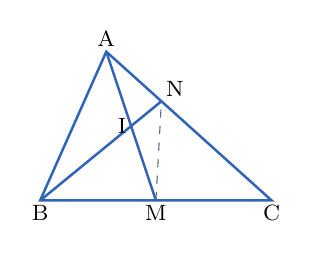
\begin{tikzpicture}[scale=0.7]
\coordinate (B) at (0,0); \coordinate (C) at (4.2,0); \coordinate (A) at (1.2,2.7); \coordinate (M) at (2.1,0); \coordinate (I) at (1.65,1.35); \coordinate (N) at (2.2,1.8);
\draw[geo] (A)--(B)--(C)--cycle; \draw[geo] (A)--(M) (B)--(N);
\draw[dashed,Slate] (M)--(N);
\node[lbl,above] at (A){A}; \node[lbl,below] at (B){B}; \node[lbl,below] at (C){C}; \node[lbl,below] at (M){M}; \node[lbl,left] at (I){I}; \node[lbl,above right] at (N){N};
\end{tikzpicture}
\end{minipage}
\end{probbox}
\probsol{
Join M to N.\par Since $AI=IM$, $S_{ABI}=S_{MBI}$ and $S_{AIN}=S_{MIN}$.\par Adding: $S_{ABN}=S_{MBN}$.\par
Since $BM=MC$, $S_{MBN}=S_{MNC}$.\par Hence $S_{BNC}=2\times S_{ABN}$.\par
ABN and CBN share the height from B, so $NC=2\times AN$, i.e.\par $AN=\dfrac13AC$.
\dapso{Shown as required.}}
\gap
\begin{probbox}{35}{\stars{2}}
Triangle ABC has area $90$ cm$^2$. M is on BC with $BM=\dfrac13BC$, N on CA with $CN=\dfrac13CA$, and P on AB with $AP=\dfrac13AB$. Find $S_{MNP}$.
\end{probbox}
\probsol{
Triangle APN: $S_{APC}=\dfrac13\times90=30$; $AN=\dfrac23AC$, so $S_{APN}=\dfrac23\times30=20$ cm$^2$.\par
Likewise $S_{BMP}=20$ and $S_{CNM}=20$ cm$^2$.\par So $S_{MNP}=90-3\times20=30$ cm$^2$.
\dapso{$30$ cm$^2$.}}
\gap
\begin{probbox}{36}{\stars{1}}
Triangle ABC has area $60$ cm$^2$. M on BC has $BM=\dfrac{1}{3}BC$; N on AM has $AN=\dfrac{1}{2}AM$. Find the areas of ABN, NBM and ANC.
\end{probbox}
\probsol{
$S_{ABM}=60\times\dfrac{1}{3}=20$ cm$^2$; $S_{AMC}=40$ cm$^2$.\par ABN and ABM share the height from B: $S_{ABN}=20\times\dfrac{1}{2}=10$ cm$^2$.\par $S_{NBM}=20-10=10$ cm$^2$.\par ANC and AMC share the height from C: $S_{ANC}=40\times\dfrac{1}{2}=20$ cm$^2$.
\dapso{$S_{ABN}=10$, $S_{NBM}=10$, $S_{ANC}=20$ (cm$^2$).}}
\gap
\begin{probbox}{37}{\stars{1}}
Triangle ABC has area $96$ cm$^2$. M on BC has $BM=\dfrac{1}{4}BC$; N on AM has $AN=\dfrac{2}{3}AM$. Find the areas of ABN, NBM and ANC.
\end{probbox}
\probsol{
$S_{ABM}=96\times\dfrac{1}{4}=24$ cm$^2$; $S_{AMC}=72$ cm$^2$.\par ABN and ABM share the height from B: $S_{ABN}=24\times\dfrac{2}{3}=16$ cm$^2$.\par $S_{NBM}=24-16=8$ cm$^2$.\par ANC and AMC share the height from C: $S_{ANC}=72\times\dfrac{2}{3}=48$ cm$^2$.
\dapso{$S_{ABN}=16$, $S_{NBM}=8$, $S_{ANC}=48$ (cm$^2$).}}
\gap
\begin{probbox}{38}{\stars{1}}
Triangle ABC has area $150$ cm$^2$. M on BC has $BM=\dfrac{2}{5}BC$; N on AM has $AN=\dfrac{3}{5}AM$. Find the areas of ABN, NBM and ANC.
\end{probbox}
\probsol{
$S_{ABM}=150\times\dfrac{2}{5}=60$ cm$^2$; $S_{AMC}=90$ cm$^2$.\par ABN and ABM share the height from B: $S_{ABN}=60\times\dfrac{3}{5}=36$ cm$^2$.\par $S_{NBM}=60-36=24$ cm$^2$.\par ANC and AMC share the height from C: $S_{ANC}=90\times\dfrac{3}{5}=54$ cm$^2$.
\dapso{$S_{ABN}=36$, $S_{NBM}=24$, $S_{ANC}=54$ (cm$^2$).}}
\gap
\begin{probbox}{39}{\stars{1}}
M on AB has $AM=\dfrac{1}{2}AB$ and N on AC has $AN=\dfrac{2}{5}AC$. Triangle AMN has area $10$ cm$^2$. Find the area of ABC.
\end{probbox}
\probsol{
Join M to C.\par AMN and AMC share the height from M: $S_{AMC}=10:\dfrac{2}{5}=25$ cm$^2$.\par AMC and ABC share the height from C: $S_{ABC}=25:\dfrac{1}{2}=50$ cm$^2$.
\dapso{$50$ cm$^2$.}}
\gap
\begin{probbox}{40}{\stars{1}}
M on AB has $AM=\dfrac{3}{4}AB$ and N on AC has $AN=\dfrac{2}{3}AC$. Triangle AMN has area $18$ cm$^2$. Find the area of ABC.
\end{probbox}
\probsol{
Join M to C.\par AMN and AMC share the height from M: $S_{AMC}=18:\dfrac{2}{3}=27$ cm$^2$.\par AMC and ABC share the height from C: $S_{ABC}=27:\dfrac{3}{4}=36$ cm$^2$.
\dapso{$36$ cm$^2$.}}
\gap
\begin{probbox}{41}{\stars{1}}
Triangle ABC has area $12$ cm$^2$. Extend AB beyond B by $BD=AB$ and AC beyond C by $CE=2\times AC$. Find the area of ADE.
\end{probbox}
\probsol{
$AD=2\times AB$, $AE=3\times AC$.\par Join D to C.\par ADC and ABC share the height from C: $S_{ADC}=12\times2=24$ cm$^2$.\par ADE and ADC share the height from D: $S_{ADE}=24\times3=72$ cm$^2$.
\dapso{$72$ cm$^2$.}}
\gap
\begin{probbox}{42}{\stars{1}}
Triangle ABC has area $15$ cm$^2$. Extend AB beyond B by $BD=2\times AB$ and AC beyond C by $CE=2\times AC$. Find the area of ADE.
\end{probbox}
\probsol{
$AD=3\times AB$, $AE=3\times AC$.\par Join D to C.\par ADC and ABC share the height from C: $S_{ADC}=15\times3=45$ cm$^2$.\par ADE and ADC share the height from D: $S_{ADE}=45\times3=135$ cm$^2$.
\dapso{$135$ cm$^2$.}}
\gap
\begin{probbox}{43}{\stars{2}}
Triangle ABC has area $80$ cm$^2$. M, N, P lie on AB, BC, CA with $AM=\dfrac{1}{4}AB$, $BN=\dfrac{1}{4}BC$, $CP=\dfrac{1}{4}CA$. Find the area of MNP.
\end{probbox}
\probsol{
In triangle AMP: $AM=\dfrac{1}{4}AB$, $AP=\dfrac{3}{4}AC$.\par As before (join M to C): $S_{AMP}=80\times\dfrac{1}{4}\times\dfrac{3}{4}=15$ cm$^2$.\par Likewise $S_{BNM}=S_{CPN}=15$ cm$^2$.\par $S_{MNP}=80-3\times15=35$ cm$^2$.
\dapso{$35$ cm$^2$.}}
\gap
\begin{probbox}{44}{\stars{2}}
Triangle ABC has area $72$ cm$^2$. M, N, P lie on AB, BC, CA with $AM=\dfrac{1}{3}AB$, $BN=\dfrac{1}{3}BC$, $CP=\dfrac{1}{3}CA$. Find the area of MNP.
\end{probbox}
\probsol{
In triangle AMP: $AM=\dfrac{1}{3}AB$, $AP=\dfrac{2}{3}AC$.\par As before (join M to C): $S_{AMP}=72\times\dfrac{1}{3}\times\dfrac{2}{3}=16$ cm$^2$.\par Likewise $S_{BNM}=S_{CPN}=16$ cm$^2$.\par $S_{MNP}=72-3\times16=24$ cm$^2$.
\dapso{$24$ cm$^2$.}}
\gap
\begin{probbox}{45}{\stars{1}}
In triangle ABC, M on BC has $BM:MC=3:1$. Triangle ABM is $20$ cm$^2$ larger than AMC. Find the area of ABC.
\end{probbox}
\probsol{
ABM and AMC share the height from A, so $S_{ABM}:S_{AMC}=3:1$.\par The difference of $2$ parts is $20$ cm$^2$; one part is $10$ cm$^2$.\par $S_{ABC}=10\times4=40$ cm$^2$.
\dapso{$40$ cm$^2$.}}
\gap
\begin{probbox}{46}{\stars{1}}
In triangle ABC, M on BC has $BM:MC=5:2$. Triangle ABM is $24$ cm$^2$ larger than AMC. Find the area of ABC.
\end{probbox}
\probsol{
ABM and AMC share the height from A, so $S_{ABM}:S_{AMC}=5:2$.\par The difference of $3$ parts is $24$ cm$^2$; one part is $8$ cm$^2$.\par $S_{ABC}=8\times7=56$ cm$^2$.
\dapso{$56$ cm$^2$.}}
\gap
\begin{probbox}{47}{\stars{1}}
Rectangle ABCD has $AB=24$ cm, $BC=16$ cm. M on AB has $AM=8$ cm; N on BC has $BN=6$ cm. Find the area of triangle DMN.
\end{probbox}
\probsol{
$S_{ABCD}=24\times16=384$ cm$^2$.\par $S_{AMD}=64$, $S_{MBN}=48$, $S_{NCD}=120$ cm$^2$.\par $S_{DMN}=384-64-48-120=152$ cm$^2$.
\dapso{$152$ cm$^2$.}}
\gap
\begin{probbox}{48}{\stars{1}}
Rectangle ABCD has $AB=30$ cm, $BC=20$ cm. M on AB has $AM=12$ cm; N on BC has $BN=10$ cm. Find the area of triangle DMN.
\end{probbox}
\probsol{
$S_{ABCD}=30\times20=600$ cm$^2$.\par $S_{AMD}=120$, $S_{MBN}=90$, $S_{NCD}=150$ cm$^2$.\par $S_{DMN}=600-120-90-150=240$ cm$^2$.
\dapso{$240$ cm$^2$.}}
\gap
\begin{probbox}{49}{\stars{1}}
Rectangle ABCD has $AB=18$ cm, $BC=12$ cm. M on AB has $AM=6$ cm; N on BC has $BN=4$ cm. Find the area of triangle DMN.
\end{probbox}
\probsol{
$S_{ABCD}=18\times12=216$ cm$^2$.\par $S_{AMD}=36$, $S_{MBN}=24$, $S_{NCD}=72$ cm$^2$.\par $S_{DMN}=216-36-24-72=84$ cm$^2$.
\dapso{$84$ cm$^2$.}}
\gap
\begin{probbox}{50}{\stars{1}}
Triangle ABC has $BC=16$ cm. Extending BC beyond C by $5$ cm gives a triangle $25$ cm$^2$ larger. Find the area of ABC.
\end{probbox}
\probsol{
The extra part is a triangle with base $5$ cm and the same height from A.\par Height: $25\times2:5=10$ cm.\par $S_{ABC}=16\times10:2=80$ cm$^2$.
\dapso{$80$ cm$^2$.}}
\clearpage
\titlehead
\begingroup\setbox0=\vbox{\section*{Trapezia and Their Area}}\endgroup
\chapterhead{13}{Trapezia and Their Area}

\shead{Two parallel bases}
\begin{knowbox}
\begin{minipage}[t]{0.6\linewidth}
A \textbf{trapezium} is a quadrilateral with \emph{one pair of parallel opposite sides}: the \textbf{longer base} and the \textbf{shorter base}. The other two sides are the \textbf{legs}. A trapezium with one leg perpendicular to the bases is a \textbf{right trapezium}.\par
\smallskip
The \textbf{height} is the distance between the bases.
\[S=\frac{(a+b)\times h}{2}\qquad h=\frac{S\times2}{a+b}\qquad a+b=\frac{S\times2}{h}\]
\textbf{The diagonals.} In trapezium ABCD (AB parallel to CD), triangles ACD and BCD share base CD and have equal heights, so $S_{ACD}=S_{BCD}$; removing the common part gives $S_{AOD}=S_{BOC}$.
\end{minipage}\hfill
\begin{minipage}[t]{0.36\linewidth}\vspace{4pt}\centering
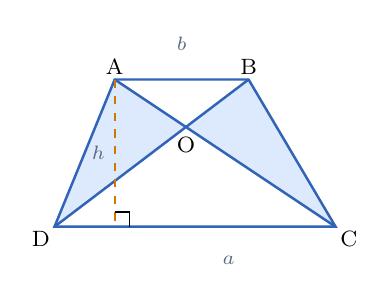
\begin{tikzpicture}[scale=0.85]
\coordinate (D) at (0,0); \coordinate (C) at (4.2,0); \coordinate (A) at (0.9,2.2); \coordinate (B) at (2.9,2.2); \coordinate (H) at (0.9,0);
\coordinate (O) at (intersection of A--C and B--D);
\fill[tmBlue!18] (A)--(O)--(D)--cycle; \fill[tmBlue!18] (B)--(O)--(C)--cycle;
\draw[geo] (A)--(B)--(C)--(D)--cycle; \draw[geo] (A)--(C) (B)--(D);
\draw[dashed,tmOrange!80!black,line width=0.7pt] (A)--(H); \ramark{H}{C}{A}
\node[lbl,above] at (A){A}; \node[lbl,above] at (B){B}; \node[lbl,below right] at (C){C}; \node[lbl,below left] at (D){D}; \node[lbl,below=2pt] at (O){O};
\node[dim,left] at (0.9,1.1){$h$}; \node[dim,above=7pt] at (1.9,2.2){$b$}; \node[dim,below=7pt] at (2.6,0){$a$};
\end{tikzpicture}
\end{minipage}
\end{knowbox}
\gap
\begin{exbox}{\ExWord\ 1}
Find the area of a trapezium with bases $12$ cm and $8$ cm and height $5$ cm.
\guide
$S=(12+8)\times5:2=50$ cm$^2$.
\dapso{$50$ cm$^2$.}
\end{exbox}
\gap
\begin{exbox}{\ExWord\ 2}
A trapezium-shaped field has a longer base of $120$ m; the shorter base is $\dfrac23$ of the longer, and the height is the mean of the two bases. Every $100$ m$^2$ yields $64$ kg of paddy. How much paddy does the field yield?
\guide
Shorter base: $120\times\dfrac23=80$ m.\par Height: $(120+80):2=100$ m.\par
Area: $(120+80)\times100:2=10\,000$ m$^2$.\par Paddy: $64\times(10\,000:100)=6\,400$ kg.
\dapso{$6\,400$ kg.}
\end{exbox}
\gap
\begin{exbox}{\ExWord\ 3}
A trapezium has area $60$ cm$^2$ and height $6$ cm; the longer base is $4$ cm longer than the shorter. Find both bases.
\guide
Sum of the bases: $60\times2:6=20$ cm.\par This is a sum-and-difference problem: longer base $(20+4):2=12$ cm, shorter $8$ cm.
\dapso{$12$ cm and $8$ cm.}
\end{exbox}
\gap
\begin{exbox}{\ExWord\ 4}
Trapezium ABCD has shorter base $AB=6$ cm, longer base $CD=9$ cm and height $4$ cm. Find the areas of triangles ABD and BCD, and show that $S_{AOD}=S_{BOC}$ (O is where the diagonals cross).
\guide
Both triangles have the trapezium's height: $S_{ABD}=6\times4:2=12$ cm$^2$ and $S_{BCD}=9\times4:2=18$ cm$^2$.\par
$S_{ACD}=S_{BCD}=18$ cm$^2$ (same base CD, same height).\par Removing their common part, triangle OCD, gives $S_{AOD}=S_{BOC}$.
\dapso{$12$ cm$^2$; $18$ cm$^2$.}
\end{exbox}
\dividerbar{Practice}
\begin{probbox}{1}{\relax}
Find the area of a trapezium with bases $a$, $b$ and height $h$:
\begin{cols2}
\pa{a} $a=14$ cm, $b=6$ cm, $h=7$ cm; & \pa{b} $a=2.8$ m, $b=1.6$ m, $h=0.5$ m;\\
\pa{c} $a=\dfrac34$ dm, $b=\dfrac12$ dm, $h=\dfrac23$ dm; & \pa{d} $a=1.5$ dm, $b=9$ cm, $h=8$ cm.
\end{cols2}
\end{probbox}
\probsol{
\pa{a} $(14+6)\times7:2=70$ cm$^2$.\par \pa{b} $(2.8+1.6)\times0.5:2=1.1$ m$^2$.\par \pa{c} $\left(\dfrac34+\dfrac12\right)\times\dfrac23:2=\dfrac5{12}$ dm$^2$.\par \pa{d} $1.5$ dm $=15$ cm; $(15+9)\times8:2=96$ cm$^2$.
\dapso{$70$ cm$^2$; $1.1$ m$^2$; $\dfrac5{12}$ dm$^2$; $96$ cm$^2$.}}
\gap
\begin{probbox}{2}{\relax}
A right trapezium has bases $10$ cm and $7$ cm, and the leg perpendicular to them is $6$ cm. Find its area.
\end{probbox}
\probsol{
The perpendicular leg is the height: $S=(10+7)\times6:2=51$ cm$^2$.
\dapso{$51$ cm$^2$.}}
\gap
\begin{probbox}{3}{\relax}
A trapezium has area $72$ cm$^2$ and bases $10$ cm and $14$ cm. Find its height.
\end{probbox}
\probsol{
$h=72\times2:(10+14)=6$ cm.
\dapso{$6$ cm.}}
\gap
\begin{probbox}{4}{\relax}
A trapezium has area $45$ m$^2$, height $5$ m and shorter base $7$ m. Find the longer base.
\end{probbox}
\probsol{
Sum of bases: $45\times2:5=18$ m.\par Longer base: $18-7=11$ m.
\dapso{$11$ m.}}
\gap
\begin{probbox}{5}{\relax}
A trapezium-shaped field has bases $60$ m and $40$ m and height $30$ m. Every $100$ m$^2$ yields $70$ kg of paddy. How much paddy does the field yield?
\end{probbox}
\probsol{
Area: $(60+40)\times30:2=1\,500$ m$^2$.\par Paddy: $70\times15=1\,050$ kg.
\dapso{$1\,050$ kg.}}
\gap
\begin{probbox}{6}{\relax}
A trapezium's bases add up to $48$ cm; the shorter is $\dfrac35$ of the longer, and the height is $\dfrac14$ of the longer base. Find its area.
\end{probbox}
\probsol{
Longer base: $48:(3+5)\times5=30$ cm; height: $30\times\dfrac14=7.5$ cm.\par $S=48\times7.5:2=180$ cm$^2$.
\dapso{$180$ cm$^2$.}}
\gap
\begin{probbox}{7}{\relax}
A trapezium has bases $25$ cm and $15$ cm. Lengthening the longer base by $5$ cm adds $20$ cm$^2$ to the area. Find the original area.
\end{probbox}
\probsol{
The added part is a triangle with base $5$ cm and the trapezium's height: $h=20\times2:5=8$ cm.\par $S=(25+15)\times8:2=160$ cm$^2$.
\dapso{$160$ cm$^2$.}}
\gap
\begin{probbox}{8}{\relax}
Rectangle ABCD has $AB=20$ cm and $BC=12$ cm. M is on AB with $AM=8$ cm. Find the area of trapezium MBCD.
\end{probbox}
\probsol{
MBCD has bases $MB=12$ cm and $CD=20$ cm and height $BC=12$ cm: $S=(12+20)\times12:2=192$ cm$^2$.\par
\emph{Another way:} $20\times12-8\times12:2=240-48=192$ cm$^2$.
\dapso{$192$ cm$^2$.}}
\gap
\begin{probbox}{9}{\relax}
Trapezium ABCD has $AB=4$ cm, $CD=10$ cm and height $6$ cm. Find the areas of triangles ABC and ACD.
\end{probbox}
\probsol{
$S_{ABC}=4\times6:2=12$ cm$^2$;\par $S_{ACD}=10\times6:2=30$ cm$^2$.\par \emph{Check:} $12+30=42=(4+10)\times6:2$.
\dapso{$12$ cm$^2$; $30$ cm$^2$.}}
\gap
\begin{probbox}{10}{\relax}
Find the area of a trapezium with bases $15$ cm and $9$ cm and height $6$ cm.
\end{probbox}
\probsol{
$S=(15+9)\times6:2=72$ cm$^2$.
\dapso{$72$ cm$^2$.}}
\gap
\begin{probbox}{11}{\relax}
Find the area of a trapezium with bases $6.5$ cm and $3.5$ cm and height $4.2$ cm.
\end{probbox}
\probsol{
$S=(6.5+3.5)\times4.2:2=21$ cm$^2$.
\dapso{$21$ cm$^2$.}}
\gap
\begin{probbox}{12}{\relax}
Find the area of a trapezium with bases $\dfrac34$ m and $\dfrac12$ m and height $\dfrac23$ m.
\end{probbox}
\probsol{
$S=\left(\dfrac34+\dfrac12\right)\times\dfrac23:2=\dfrac54\times\dfrac23:2=\dfrac5{12}$ m$^2$.
\dapso{$\dfrac5{12}$ m$^2$.}}
\gap
\begin{probbox}{13}{\relax}
Find the area of a trapezium with bases $14$ dm and $10$ dm and height $7.5$ dm.
\end{probbox}
\probsol{
$S=(14+10)\times7.5:2=90$ dm$^2$.
\dapso{$90$ dm$^2$.}}
\gap
\begin{probbox}{14}{\relax}
Find the area of a trapezium with bases $1.2$ m and $80$ cm and height $5$ dm.
\end{probbox}
\probsol{
In decimetres: $1.2$ m $=12$ dm; $80$ cm $=8$ dm.\par $S=(12+8)\times5:2=50$ dm$^2$.
\dapso{$50$ dm$^2$.}}
\gap
\begin{probbox}{15}{\relax}
A trapezium has area $84$ cm$^2$ and bases $16$ cm and $12$ cm. Find its height.
\end{probbox}
\probsol{
Height $=$ area $\times2\,:$ sum of bases.\par $h=84\times2:(16+12)=6$ cm.
\dapso{$6$ cm.}}
\gap
\begin{probbox}{16}{\relax}
A trapezium has area $45$ cm$^2$ and bases $8.5$ cm and $6.5$ cm. Find its height.
\end{probbox}
\probsol{
Height $=$ area $\times2\,:$ sum of bases.\par $h=45\times2:(8.5+6.5)=6$ cm.
\dapso{$6$ cm.}}
\gap
\begin{probbox}{17}{\relax}
A trapezium has area $150$ cm$^2$ and bases $23$ cm and $17$ cm. Find its height.
\end{probbox}
\probsol{
Height $=$ area $\times2\,:$ sum of bases.\par $h=150\times2:(23+17)=7.5$ cm.
\dapso{$7.5$ cm.}}
\gap
\begin{probbox}{18}{\relax}
A trapezium has area $96$ cm$^2$, height $8$ cm and shorter base $10$ cm. Find the longer base.
\end{probbox}
\probsol{
Sum of bases: $96\times2:8=24$ cm.\par Longer base: $24-10=14$ cm.
\dapso{$14$ cm.}}
\gap
\begin{probbox}{19}{\relax}
A trapezium has area $63$ cm$^2$, height $7$ cm and shorter base $7.5$ cm. Find the longer base.
\end{probbox}
\probsol{
Sum of bases: $63\times2:7=18$ cm.\par Longer base: $18-7.5=10.5$ cm.
\dapso{$10.5$ cm.}}
\gap
\begin{probbox}{20}{\relax}
A trapezium has area $110$ cm$^2$, height $10$ cm and shorter base $9$ cm. Find the longer base.
\end{probbox}
\probsol{
Sum of bases: $110\times2:10=22$ cm.\par Longer base: $22-9=13$ cm.
\dapso{$13$ cm.}}
\gap
\begin{probbox}{21}{\relax}
A trapezium-shaped field has bases $80$ m and $50$ m and height $40$ m. Every $100$ m$^2$ yields $65$ kg of paddy. What is the total yield?
\end{probbox}
\probsol{
Area: $(80+50)\times40:2=2\,600$ m$^2$.\par Yield: $2\,600:100\times65=1\,690$ kg.
\dapso{$1\,690$ kg.}}
\gap
\begin{probbox}{22}{\relax}
A trapezium-shaped field has bases $150$ m and $90$ m and height $60$ m. Every $100$ m$^2$ yields $60$ kg of paddy. What is the total yield?
\end{probbox}
\probsol{
Area: $(150+90)\times60:2=7\,200$ m$^2$.\par Yield: $7\,200:100\times60=4\,320$ kg.
\dapso{$4\,320$ kg.}}
\gap
\begin{probbox}{23}{\relax}
A trapezium's bases add up to $36$ cm and differ by $8$ cm; its height is $10$ cm. Find each base and the area.
\end{probbox}
\probsol{
Longer base: $(36+8):2=22$ cm; shorter: $14$ cm.\par Area: $36\times10:2=180$ cm$^2$.
\dapso{Bases $22$ cm and $14$ cm; $180$ cm$^2$.}}
\gap
\begin{probbox}{24}{\relax}
A trapezium's bases add up to $50$ cm and differ by $14$ cm; its height is $12$ cm. Find each base and the area.
\end{probbox}
\probsol{
Longer base: $(50+14):2=32$ cm; shorter: $18$ cm.\par Area: $50\times12:2=300$ cm$^2$.
\dapso{Bases $32$ cm and $18$ cm; $300$ cm$^2$.}}
\gap
\begin{probbox}{25}{\relax}
A trapezium-shaped plot has longer base $60$ m; the shorter base is $\dfrac{2}{3}$ of it and the height is $\dfrac{1}{2}$ of it. Find the area.
\end{probbox}
\probsol{
Shorter base: $60\times\dfrac{2}{3}=40$ m.\par Height: $60\times\dfrac{1}{2}=30$ m.\par Area: $(60+40)\times30:2=1\,500$ m$^2$.
\dapso{$1\,500$ m$^2$.}}
\gap
\begin{probbox}{26}{\relax}
A trapezium-shaped plot has longer base $48$ m; the shorter base is $\dfrac{3}{4}$ of it and the height is $\dfrac{5}{8}$ of it. Find the area.
\end{probbox}
\probsol{
Shorter base: $48\times\dfrac{3}{4}=36$ m.\par Height: $48\times\dfrac{5}{8}=30$ m.\par Area: $(48+36)\times30:2=1\,260$ m$^2$.
\dapso{$1\,260$ m$^2$.}}
\gap
\begin{probbox}{27}{\relax}
Trapezium ABCD has right angles at A and D, $AB=9$ cm, $CD=15$ cm and $AD=8$ cm. Find its area.
\end{probbox}
\probsol{
AD is perpendicular to both bases, so it is the height.\par $S=(9+15)\times8:2=96$ cm$^2$.
\dapso{$96$ cm$^2$.}}
\gap
\begin{probbox}{28}{\relax}
Trapezium ABCD has right angles at A and D, $AB=4.5$ cm, $CD=7.5$ cm and $AD=6$ cm. Find its area.
\end{probbox}
\probsol{
AD is perpendicular to both bases, so it is the height.\par $S=(4.5+7.5)\times6:2=36$ cm$^2$.
\dapso{$36$ cm$^2$.}}
\gap
\begin{probbox}{29}{\relax}
Rectangle ABCD has $AB=25$ cm and $BC=14$ cm. M on AB has $AM=9$ cm. Find the areas of trapezium MBCD and triangle AMD.
\end{probbox}
\probsol{
MBCD has bases $MB=16$ cm and $CD=25$ cm and height $BC=14$ cm.\par $S_{MBCD}=(16+25)\times14:2=287$ cm$^2$.\par $S_{AMD}=9\times14:2=63$ cm$^2$.
\dapso{$S_{MBCD}=287$ cm$^2$, $S_{AMD}=63$ cm$^2$.}}
\gap
\begin{probbox}{30}{\relax}
Rectangle ABCD has $AB=30$ cm and $BC=16$ cm. M on AB has $AM=12$ cm. Find the areas of trapezium MBCD and triangle AMD.
\end{probbox}
\probsol{
MBCD has bases $MB=18$ cm and $CD=30$ cm and height $BC=16$ cm.\par $S_{MBCD}=(18+30)\times16:2=384$ cm$^2$.\par $S_{AMD}=12\times16:2=96$ cm$^2$.
\dapso{$S_{MBCD}=384$ cm$^2$, $S_{AMD}=96$ cm$^2$.}}
\dividerbar{Challenge -- Extension}
\begin{probbox}{31}{\stars{1}}
A trapezium has bases $12$ cm and $18$ cm. Lengthening the shorter base by $6$ cm turns it into a rectangle and adds $27$ cm$^2$. Find the trapezium's area.
\end{probbox}
\probsol{
The added part is a triangle with side $6$ cm and the trapezium's height: $h=27\times2:6=9$ cm.\par $S=(12+18)\times9:2=135$ cm$^2$.
\dapso{$135$ cm$^2$.}}
\gap
\begin{probbox}{32}{\stars{1}}
A trapezium-shaped field has bases adding up to $140$ m, the longer $20$ m longer than the shorter. Lengthening each base by $10$ m adds $500$ m$^2$. Find the original area and both bases.
\end{probbox}
\probsol{
The bases grow by $20$ m in total, so $h=500\times2:20=50$ m.\par $S=140\times50:2=3\,500$ m$^2$.\par
Longer base: $(140+20):2=80$ m; shorter: $60$ m.
\dapso{$3\,500$ m$^2$; $80$ m and $60$ m.}}
\gap
\begin{probbox}{33}{\stars{1}}
In trapezium ABCD, the shorter base AB is $\dfrac13$ of the longer base CD, and $S_{ABD}=15$ cm$^2$. Find the area of the trapezium.
\end{probbox}
\probsol{
ABD and BCD both have the trapezium's height, and $CD=3\times AB$, so $S_{BCD}=15\times3=45$ cm$^2$.\par $S_{ABCD}=15+45=60$ cm$^2$.
\dapso{$60$ cm$^2$.}}
\gap
\begin{probbox}{34}{\stars{2}}
Right trapezium ABCD has right angles at A and D, $AB=6$ cm, $CD=12$ cm and $AD=8$ cm. M is the midpoint of AD. Find $S_{MBC}$.
\end{probbox}
\probsol{
$S_{ABCD}=(6+12)\times8:2=72$;\par $S_{ABM}=6\times4:2=12$;\par $S_{MDC}=12\times4:2=24$ cm$^2$.\par
$S_{MBC}=72-12-24=36$ cm$^2$, exactly half the trapezium.
\dapso{$36$ cm$^2$.}}
\gap
\begin{probbox}{35}{\stars{2}}
In trapezium ABCD (AB parallel to CD), the diagonals cross at O. $S_{AOB}=4$ cm$^2$ and $S_{BOC}=8$ cm$^2$. Find the area of the trapezium.
\end{probbox}
\probsol{
AOB and BOC share the height from B, so $OC=2\times OA$.\par
By the trapezium property, $S_{AOD}=S_{BOC}=8$ cm$^2$.\par COD and AOD share the height from D and $OC=2\times OA$, so $S_{COD}=16$ cm$^2$.\par
$S_{ABCD}=4+8+8+16=36$ cm$^2$.
\dapso{$36$ cm$^2$.}}
\gap
\begin{probbox}{36}{\stars{1}}
A trapezium has bases $30$ cm and $18$ cm. Lengthening the longer base by $6$ cm (same height) adds $27$ cm$^2$. Find the original area.
\end{probbox}
\probsol{
The extra part is a triangle with base $6$ cm and the trapezium's height.\par Height: $27\times2:6=9$ cm.\par Area: $(30+18)\times9:2=216$ cm$^2$.
\dapso{$216$ cm$^2$.}}
\gap
\begin{probbox}{37}{\stars{1}}
A trapezium has bases $22$ cm and $14$ cm. Lengthening the longer base by $4$ cm (same height) adds $18$ cm$^2$. Find the original area.
\end{probbox}
\probsol{
The extra part is a triangle with base $4$ cm and the trapezium's height.\par Height: $18\times2:4=9$ cm.\par Area: $(22+14)\times9:2=162$ cm$^2$.
\dapso{$162$ cm$^2$.}}
\gap
\begin{probbox}{38}{\stars{1}}
A trapezium-shaped garden has bases summing to $90$ m, differing by $30$ m. Adding $5$ m to each base (same height) adds $200$ m$^2$. Find the original area.
\end{probbox}
\probsol{
The extra part is a trapezium with bases $5$ m and $5$ m and the same height.\par Height: $200\times2:(5+5)=40$ m.\par Original area: $90\times40:2=1\,800$ m$^2$.
\dapso{$1\,800$ m$^2$.}}
\gap
\begin{probbox}{39}{\stars{1}}
A trapezium-shaped garden has bases summing to $120$ m, differing by $40$ m. Adding $8$ m to each base (same height) adds $320$ m$^2$. Find the original area.
\end{probbox}
\probsol{
The extra part is a trapezium with bases $8$ m and $8$ m and the same height.\par Height: $320\times2:(8+8)=40$ m.\par Original area: $120\times40:2=2\,400$ m$^2$.
\dapso{$2\,400$ m$^2$.}}
\gap
\begin{probbox}{40}{\stars{1}}
In trapezium ABCD the shorter base AB is $\dfrac{1}{2}$ of the longer base CD. Triangle ABD has area $12$ cm$^2$. Find the area of the trapezium.
\end{probbox}
\probsol{
ABD and BCD have the same height (the trapezium's height).\par So $S_{ABD}=\dfrac{1}{2}S_{BCD}$.\par $S_{BCD}=12:\dfrac{1}{2}=24$ cm$^2$.\par $S_{ABCD}=36$ cm$^2$.
\dapso{$36$ cm$^2$.}}
\gap
\begin{probbox}{41}{\stars{1}}
In trapezium ABCD the shorter base AB is $\dfrac{2}{3}$ of the longer base CD. Triangle ABD has area $18$ cm$^2$. Find the area of the trapezium.
\end{probbox}
\probsol{
ABD and BCD have the same height (the trapezium's height).\par So $S_{ABD}=\dfrac{2}{3}S_{BCD}$.\par $S_{BCD}=18:\dfrac{2}{3}=27$ cm$^2$.\par $S_{ABCD}=45$ cm$^2$.
\dapso{$45$ cm$^2$.}}
\gap
\begin{probbox}{42}{\stars{2}}
Trapezium ABCD (AB parallel to CD) has diagonals meeting at O. $S_{AOB}=4$ cm$^2$ and $S_{BOC}=6$ cm$^2$. Find the area of the trapezium.
\end{probbox}
\probsol{
$S_{ABD}=S_{ABC}$ (same base AB, same height); removing AOB gives $S_{AOD}=S_{BOC}=6$ cm$^2$.\par AOB and BOC share the height from B, so $\dfrac{OA}{OC}=\dfrac{4}{6}$.\par AOD and COD share the height from D, so $S_{COD}=6\times\dfrac{6}{4}=9$ cm$^2$.\par $S_{ABCD}=4+6+6+9=25$ cm$^2$.
\dapso{$25$ cm$^2$.}}
\gap
\begin{probbox}{43}{\stars{2}}
Trapezium ABCD (AB parallel to CD) has diagonals meeting at O. $S_{AOB}=9$ cm$^2$ and $S_{BOC}=12$ cm$^2$. Find the area of the trapezium.
\end{probbox}
\probsol{
$S_{ABD}=S_{ABC}$ (same base AB, same height); removing AOB gives $S_{AOD}=S_{BOC}=12$ cm$^2$.\par AOB and BOC share the height from B, so $\dfrac{OA}{OC}=\dfrac{9}{12}$.\par AOD and COD share the height from D, so $S_{COD}=12\times\dfrac{12}{9}=16$ cm$^2$.\par $S_{ABCD}=9+12+12+16=49$ cm$^2$.
\dapso{$49$ cm$^2$.}}
\gap
\begin{probbox}{44}{\stars{2}}
Trapezium ABCD (AB parallel to CD) has diagonals meeting at O. $S_{AOB}=2$ cm$^2$ and $S_{BOC}=6$ cm$^2$. Find the area of the trapezium.
\end{probbox}
\probsol{
$S_{ABD}=S_{ABC}$ (same base AB, same height); removing AOB gives $S_{AOD}=S_{BOC}=6$ cm$^2$.\par AOB and BOC share the height from B, so $\dfrac{OA}{OC}=\dfrac{2}{6}$.\par AOD and COD share the height from D, so $S_{COD}=6\times\dfrac{6}{2}=18$ cm$^2$.\par $S_{ABCD}=2+6+6+18=32$ cm$^2$.
\dapso{$32$ cm$^2$.}}
\gap
\begin{probbox}{45}{\stars{1}}
Trapezium ABCD has right angles at A and D, $AB=8$ cm, $CD=14$ cm, $AD=10$ cm. M is the midpoint of AD. Find the area of triangle MBC.
\end{probbox}
\probsol{
$S_{ABCD}=(8+14)\times10:2=110$ cm$^2$.\par $AM=MD=5$ cm.\par $S_{MAB}=20$, $S_{MDC}=35$ cm$^2$.\par $S_{MBC}=110-20-35=55$ cm$^2$.
\dapso{$55$ cm$^2$.}}
\gap
\begin{probbox}{46}{\stars{1}}
Trapezium ABCD has right angles at A and D, $AB=5$ cm, $CD=11$ cm, $AD=12$ cm. M is the midpoint of AD. Find the area of triangle MBC.
\end{probbox}
\probsol{
$S_{ABCD}=(5+11)\times12:2=96$ cm$^2$.\par $AM=MD=6$ cm.\par $S_{MAB}=15$, $S_{MDC}=33$ cm$^2$.\par $S_{MBC}=96-15-33=48$ cm$^2$.
\dapso{$48$ cm$^2$.}}
\gap
\begin{probbox}{47}{\stars{1}}
A right trapezium has bases $10$ cm and $16$ cm. Lengthening the shorter base by $6$ cm makes a rectangle $24$ cm$^2$ larger. Find the trapezium's area.
\end{probbox}
\probsol{
The added piece is a right triangle with legs $6$ cm and the height.\par Height: $24\times2:6=4$ cm.\par Area: $(10+16)\times4:2=52$ cm$^2$.
\dapso{$52$ cm$^2$.}}
\gap
\begin{probbox}{48}{\stars{1}}
A right trapezium has bases $14$ cm and $20$ cm. Lengthening the shorter base by $6$ cm makes a rectangle $27$ cm$^2$ larger. Find the trapezium's area.
\end{probbox}
\probsol{
The added piece is a right triangle with legs $6$ cm and the height.\par Height: $27\times2:6=4.5$ cm.\par Area: $(14+20)\times4.5:2=76.5$ cm$^2$.
\dapso{$76.5$ cm$^2$.}}
\gap
\begin{probbox}{49}{\stars{1}}
A trapezium with bases $20$ cm and $16$ cm has the same area as a square of side $12$ cm. Find its height.
\end{probbox}
\probsol{
Square: $12\times12=144$ cm$^2$.\par Height: $144\times2:(20+16)=8$ cm.
\dapso{$8$ cm.}}
\gap
\begin{probbox}{50}{\stars{1}}
Diagonal AC splits trapezium ABCD (AB parallel to CD) into triangles with $S_{ABC}=24$ cm$^2$ and $S_{ACD}=40$ cm$^2$. The height is $8$ cm. Find both bases.
\end{probbox}
\probsol{
Both triangles have the trapezium's height, $8$ cm.\par $AB=24\times2:8=6$ cm.\par $CD=40\times2:8=10$ cm.
\dapso{$AB=6$ cm, $CD=10$ cm.}}
\clearpage
\titlehead
\begingroup\setbox0=\vbox{\section*{Circles: Circumference and Area}}\endgroup
\chapterhead{14}{Circles: Circumference and Area}

\shead{Centre, radius, diameter}
\begin{knowbox}
\begin{minipage}[t]{0.64\linewidth}
Every point on a \textbf{circle} is the same distance from the \textbf{centre} O. A segment from the centre to the circle is a \textbf{radius} $r$; a segment through the centre joining two points of the circle is a \textbf{diameter} $d$, and $d=r\times2$.\par
\smallskip
We use the number $3.14$ (called ``pi'') to calculate:
\[C=d\times3.14=r\times2\times3.14\qquad\qquad S=r\times r\times3.14\]
\begin{itemize}[leftmargin=1.4em,itemsep=2pt]
\item Given the circumference: $d=C:3.14$.
\item Given the area: find $r\times r=S:3.14$, then the number $r$.
\item If the radius is multiplied by $k$, the circumference is multiplied by $k$ and the area by $k\times k$.
\end{itemize}
\end{minipage}\hfill
\begin{minipage}[t]{0.32\linewidth}\vspace{6pt}\centering
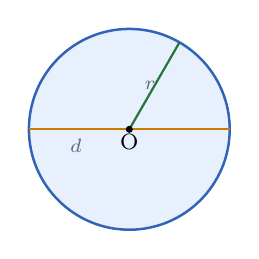
\begin{tikzpicture}[scale=0.85]
\fill[tmBlue!12] (0,0) circle (1.5); \draw[geo] (0,0) circle (1.5);
\draw[line width=0.8pt,tmOrange!80!black] (-1.5,0)--(1.5,0);
\draw[line width=0.8pt,tmGreen!70!black] (0,0)--(60:1.5);
\fill (0,0) circle (1.5pt); \node[lbl,below] at (0,0){O};
\node[dim,above left] at (40:0.7){$r$}; \node[dim,below] at (-0.8,0){$d$};
\end{tikzpicture}
\end{minipage}
\end{knowbox}
\gap
\begin{exbox}{\ExWord\ 1}
Find the circumference and area of a circle of radius $5$ cm.
\guide
$C=5\times2\times3.14=31.4$ cm.\par $S=5\times5\times3.14=78.5$ cm$^2$.
\dapso{$31.4$ cm; $78.5$ cm$^2$.}
\end{exbox}
\gap
\begin{exbox}{\ExWord\ 2}
A circle has circumference $18.84$ dm. Find its area.
\guide
Diameter: $18.84:3.14=6$ dm; radius: $3$ dm.\par $S=3\times3\times3.14=28.26$ dm$^2$.
\dapso{$28.26$ dm$^2$.}
\end{exbox}
\gap
\begin{exbox}{\ExWord\ 3}
\begin{minipage}[t]{0.66\linewidth}
A square has side $10$ cm. A circle inside it touches all four sides. Find the shaded area (the part of the square outside the circle).
\end{minipage}\hfill
\begin{minipage}[t]{0.3\linewidth}\vspace{0pt}\centering
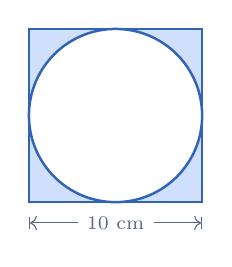
\begin{tikzpicture}[scale=0.22]
\fill[shade] (0,0) rectangle (10,10); \fill[white] (5,5) circle (5);
\draw[geo] (0,0) rectangle (10,10); \draw[geo] (5,5) circle (5);
\draw[|<->|,Slate] (0,-1.2)--node[fill=white,dim]{$10$ cm}(10,-1.2);
\end{tikzpicture}
\end{minipage}
\guide
The circle's diameter equals the side of the square: $d=10$ cm, $r=5$ cm.\par
$S_\text{square}=10\times10=100$ cm$^2$;\par $S_\text{circle}=5\times5\times3.14=78.5$ cm$^2$.\par
Shaded part: $100-78.5=21.5$ cm$^2$.
\dapso{$21.5$ cm$^2$.}
\end{exbox}
\gap
\begin{exbox}{\ExWord\ 4}
A cart wheel has a diameter of $0.6$ m. How far does the cart travel when the wheel turns $100$ times?
\guide
Each turn moves the cart by the wheel's circumference: $0.6\times3.14=1.884$ m.\par
$100$ turns: $1.884\times100=188.4$ m.
\dapso{$188.4$ m.}
\end{exbox}
\dividerbar{Practice}
\begin{probbox}{1}{\relax}
Find the circumference and area of a circle with:
\begin{cols3}
\pa{a} $r=3$ cm; & \pa{b} $r=0.5$ dm; & \pa{c} $d=8$ m.
\end{cols3}
\end{probbox}
\probsol{
\pa{a} $C=18.84$ cm; $S=28.26$ cm$^2$.\par \pa{b} $C=3.14$ dm; $S=0.785$ dm$^2$.\par \pa{c} $C=25.12$ m; $r=4$ m, $S=50.24$ m$^2$.
\dapso{See above.}}
\gap
\begin{probbox}{2}{\relax}
A circle has circumference $12.56$ cm. Find its radius and area.
\end{probbox}
\probsol{
$d=12.56:3.14=4$ cm; $r=2$ cm.\par $S=2\times2\times3.14=12.56$ cm$^2$.
\dapso{$r=2$ cm; $S=12.56$ cm$^2$.}}
\gap
\begin{probbox}{3}{\relax}
A bicycle wheel has a diameter of $65$ cm. How many kilometres does the bicycle travel in $1\,000$ turns of the wheel?
\end{probbox}
\probsol{
Each turn: $65\times3.14=204.1$ cm.\par $1\,000$ turns: $204\,100$ cm $=2.041$ km.
\dapso{$2.041$ km.}}
\gap
\begin{probbox}{4}{\relax}
A car wheel travels $1\,099$ m in $500$ turns. Find its diameter.
\end{probbox}
\probsol{
Circumference: $1\,099:500=2.198$ m.\par Diameter: $2.198:3.14=0.7$ m.
\dapso{$0.7$ m.}}
\gap
\begin{probbox}{5}{\relax}
The minute hand of a clock is $10$ cm long. How far does its tip travel in $1$ hour? In $15$ minutes?
\end{probbox}
\probsol{
In $1$ hour the tip goes once round: $10\times2\times3.14=62.8$ cm.\par In $15$ minutes, a quarter turn: $62.8:4=15.7$ cm.
\dapso{$62.8$ cm; $15.7$ cm.}}
\gap
\begin{probbox}{6}{\relax}
Find the area and perimeter of a semicircle with diameter $8$ cm.
\end{probbox}
\probsol{
$S=4\times4\times3.14:2=25.12$ cm$^2$.\par The perimeter is half the circle plus the diameter: $8\times3.14:2+8=20.56$ cm.
\dapso{$25.12$ cm$^2$; $20.56$ cm.}}
\gap
\begin{probbox}{7}{\relax}
A round flower bed has a radius of $10$ m. A path $1$ m wide is built all round it. Find the area of the path.
\end{probbox}
\probsol{
The outer circle has radius $11$ m.\par Path: $11\times11\times3.14-10\times10\times3.14=(121-100)\times3.14=65.94$ m$^2$.
\dapso{$65.94$ m$^2$.}}
\gap
\begin{probbox}{8}{\relax}
A square sits inside a circle of radius $5$ cm with its four corners on the circle. Find the area of the part of the circle outside the square.
\end{probbox}
\probsol{
The square's diagonals are diameters, $10$ cm long, and split it into $4$ right-angled triangles with sides $5$ cm: $S_\text{square}=4\times5\times5:2=50$ cm$^2$.\par
$S_\text{circle}=78.5$ cm$^2$.\par Required part: $78.5-50=28.5$ cm$^2$.
\dapso{$28.5$ cm$^2$.}}
\gap
\begin{probbox}{9}{\relax}
If the radius of a circle is multiplied by $3$, by how many times are its circumference and area multiplied? Check with $r=1$ cm.
\end{probbox}
\probsol{
The circumference is multiplied by $3$ and the area by $3\times3=9$.\par Example: $r=1$: $C=6.28$, $S=3.14$; $r=3$: $C=18.84=6.28\times3$, $S=28.26=3.14\times9$.
\dapso{$3$ times; $9$ times.}}
\gap
\begin{probbox}{10}{\relax}
Find the circumference and area of a circle of radius $3$ cm.
\end{probbox}
\probsol{
$C=3\times2\times3.14=18.84$ cm.\par $S=3\times3\times3.14=28.26$ cm$^2$.
\dapso{$C=18.84$ cm; $S=28.26$ cm$^2$.}}
\gap
\begin{probbox}{11}{\relax}
Find the circumference and area of a circle of radius $2.5$ cm.
\end{probbox}
\probsol{
$C=2.5\times2\times3.14=15.7$ cm.\par $S=2.5\times2.5\times3.14=19.625$ cm$^2$.
\dapso{$C=15.7$ cm; $S=19.625$ cm$^2$.}}
\gap
\begin{probbox}{12}{\relax}
Find the circumference and area of a circle of radius $0.8$ m.
\end{probbox}
\probsol{
$C=0.8\times2\times3.14=5.024$ m.\par $S=0.8\times0.8\times3.14=2.0096$ m$^2$.
\dapso{$C=5.024$ m; $S=2.0096$ m$^2$.}}
\gap
\begin{probbox}{13}{\relax}
Find the circumference and area of a circle of radius $12$ dm.
\end{probbox}
\probsol{
$C=12\times2\times3.14=75.36$ dm.\par $S=12\times12\times3.14=452.16$ dm$^2$.
\dapso{$C=75.36$ dm; $S=452.16$ dm$^2$.}}
\gap
\begin{probbox}{14}{\relax}
Find the circumference and area of a circle of diameter $10$ cm.
\end{probbox}
\probsol{
$C=10\times3.14=31.4$ cm.\par Radius: $10:2=5$ cm.\par $S=5\times5\times3.14=78.5$ cm$^2$.
\dapso{$C=31.4$ cm; $S=78.5$ cm$^2$.}}
\gap
\begin{probbox}{15}{\relax}
Find the circumference and area of a circle of diameter $4.2$ cm.
\end{probbox}
\probsol{
$C=4.2\times3.14=13.188$ cm.\par Radius: $4.2:2=2.1$ cm.\par $S=2.1\times2.1\times3.14=13.8474$ cm$^2$.
\dapso{$C=13.188$ cm; $S=13.8474$ cm$^2$.}}
\gap
\begin{probbox}{16}{\relax}
Find the circumference and area of a circle of diameter $2.4$ m.
\end{probbox}
\probsol{
$C=2.4\times3.14=7.536$ m.\par Radius: $2.4:2=1.2$ m.\par $S=1.2\times1.2\times3.14=4.5216$ m$^2$.
\dapso{$C=7.536$ m; $S=4.5216$ m$^2$.}}
\gap
\begin{probbox}{17}{\relax}
A circle has circumference $43.96$ cm. Find its radius and area.
\end{probbox}
\probsol{
Diameter: $43.96:3.14=14$ cm.\par Radius: $14:2=7$ cm.\par $S=7\times7\times3.14=153.86$ cm$^2$.
\dapso{$r=7$ cm; $S=153.86$ cm$^2$.}}
\gap
\begin{probbox}{18}{\relax}
A circle has circumference $21.98$ cm. Find its radius and area.
\end{probbox}
\probsol{
Diameter: $21.98:3.14=7$ cm.\par Radius: $7:2=3.5$ cm.\par $S=3.5\times3.5\times3.14=38.465$ cm$^2$.
\dapso{$r=3.5$ cm; $S=38.465$ cm$^2$.}}
\gap
\begin{probbox}{19}{\relax}
A circle has circumference $6.28$ m. Find its radius and area.
\end{probbox}
\probsol{
Diameter: $6.28:3.14=2$ m.\par Radius: $2:2=1$ m.\par $S=1\times1\times3.14=3.14$ m$^2$.
\dapso{$r=1$ m; $S=3.14$ m$^2$.}}
\gap
\begin{probbox}{20}{\relax}
A circle has area $113.04$ cm$^2$. Find its radius and circumference.
\end{probbox}
\probsol{
$r\times r=113.04:3.14=36$.\par Since $6\times6=36$, $r=6$ cm.\par $C=6\times2\times3.14=37.68$ cm.
\dapso{$r=6$ cm; $C=37.68$ cm.}}
\gap
\begin{probbox}{21}{\relax}
A circle has area $12.56$ m$^2$. Find its radius and circumference.
\end{probbox}
\probsol{
$r\times r=12.56:3.14=4$.\par Since $2\times2=4$, $r=2$ m.\par $C=2\times2\times3.14=12.56$ m.
\dapso{$r=2$ m; $C=12.56$ m.}}
\gap
\begin{probbox}{22}{\relax}
A wheel has diameter $0.5$ m. How far does it travel in $200$ turns?
\end{probbox}
\probsol{
One turn: $0.5\times3.14=1.57$ m.\par $200$ turns: $1.57\times200=314$ m.
\dapso{$314$ m.}}
\gap
\begin{probbox}{23}{\relax}
A wheel has diameter $0.7$ m. How far does it travel in $1\,000$ turns?
\end{probbox}
\probsol{
One turn: $0.7\times3.14=2.198$ m.\par $1\,000$ turns: $2.198\times1\,000=2\,198$ m.
\dapso{$2\,198$ m.}}
\gap
\begin{probbox}{24}{\relax}
A bicycle wheel travels $816.4$ m in $400$ turns. Find its diameter.
\end{probbox}
\probsol{
One turn: $816.4:400=2.041$ m.\par Diameter: $2.041:3.14=0.65$ m.
\dapso{$0.65$ m.}}
\gap
\begin{probbox}{25}{\relax}
Find the area and perimeter of a semicircle with diameter $10$ cm.
\end{probbox}
\probsol{
Area: $5\times5\times3.14:2=39.25$ cm$^2$.\par Arc: $10\times3.14:2=15.7$ cm.\par Perimeter (with the diameter): $15.7+10=25.7$ cm.
\dapso{$S=39.25$ cm$^2$; perimeter $25.7$ cm.}}
\gap
\begin{probbox}{26}{\relax}
Find the area and perimeter of a semicircle with diameter $6$ cm.
\end{probbox}
\probsol{
Area: $3\times3\times3.14:2=14.13$ cm$^2$.\par Arc: $6\times3.14:2=9.42$ cm.\par Perimeter (with the diameter): $9.42+6=15.42$ cm.
\dapso{$S=14.13$ cm$^2$; perimeter $15.42$ cm.}}
\gap
\begin{probbox}{27}{\relax}
A ceiling-fan blade is $0.6$ m long from the centre. Find the area of the circle its tip sweeps out.
\end{probbox}
\probsol{
Radius $r=0.6$ m.\par $S=0.6\times0.6\times3.14=1.1304$ m$^2$.
\dapso{$1.1304$ m$^2$.}}
\gap
\begin{probbox}{28}{\relax}
A round pond has diameter $20$ m. Fencing costs $50\,000$ dong per metre. How much does it cost to fence the pond?
\end{probbox}
\probsol{
Circumference: $20\times3.14=62.8$ m.\par Cost: $50\,000\times62.8=3\,140\,000$ dong.
\dapso{$3\,140\,000$ dong.}}
\gap
\begin{probbox}{29}{\relax}
Find the area of a quarter circle of radius $4$ cm.
\end{probbox}
\probsol{
Whole circle: $4\times4\times3.14=50.24$ cm$^2$.\par Quarter: $50.24:4=12.56$ cm$^2$.
\dapso{$12.56$ cm$^2$.}}
\gap
\begin{probbox}{30}{\relax}
Find the area of a quarter circle of radius $10$ cm.
\end{probbox}
\probsol{
Whole circle: $10\times10\times3.14=314$ cm$^2$.\par Quarter: $314:4=78.5$ cm$^2$.
\dapso{$78.5$ cm$^2$.}}
\dividerbar{Challenge -- Extension}
\begin{probbox}{31}{\stars{1}}
A circle has area $50.24$ cm$^2$. Find its circumference.
\end{probbox}
\probsol{
$r\times r=50.24:3.14=16$, so $r=4$ cm.\par $C=4\times2\times3.14=25.12$ cm.
\dapso{$25.12$ cm.}}
\gap
\begin{probbox}{32}{\stars{1}}
If a circle's radius grows by $2$ cm, by how much does its circumference grow? Does the answer depend on the original radius?
\end{probbox}
\probsol{
The increase is $(r+2)\times2\times3.14-r\times2\times3.14=2\times2\times3.14=12.56$ cm, whatever the original radius.
\dapso{$12.56$ cm; it does not depend on it.}}
\gap
\begin{probbox}{33}{\stars{1}}
A large semicircle has diameter $AB=12$ cm. M is the midpoint of AB, and two small semicircles are drawn on AM and MB. Compare the length of the large arc with the total length of the two small arcs.
\end{probbox}
\probsol{
Large arc: $12\times3.14:2=18.84$ cm.\par Each small arc: $6\times3.14:2=9.42$ cm; together $18.84$ cm.\par They are equal.
\dapso{Equal ($18.84$ cm).}}
\gap
\begin{probbox}{34}{\stars{1}}
Two circles share centre O, with radii $3$ cm and $5$ cm. Find the area between them (the ring).
\end{probbox}
\probsol{
$S=5\times5\times3.14-3\times3\times3.14=(25-9)\times3.14=50.24$ cm$^2$.
\dapso{$50.24$ cm$^2$.}}
\gap
\begin{probbox}{35}{\stars{2}}
\begin{minipage}[t]{0.66\linewidth}
Square ABCD has side $8$ cm. Four quarter circles of radius $4$ cm are drawn with centres at the four corners. Find the shaded area.
\end{minipage}\hfill
\begin{minipage}[t]{0.3\linewidth}\vspace{0pt}\centering
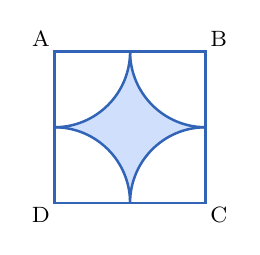
\begin{tikzpicture}[scale=0.24]
\fill[shade] (0,0) rectangle (8,8);
\foreach \x/\y/\a in {0/0/0,8/0/90,8/8/180,0/8/270}{\fill[white] (\x,\y) -- ++(\a:4) arc (\a:\a+90:4) -- cycle; \draw[geo] (\x,\y) ++(\a:4) arc (\a:\a+90:4);}
\draw[geo] (0,0) rectangle (8,8);
\node[lbl,below left] at (0,0){D}; \node[lbl,below right] at (8,0){C}; \node[lbl,above right] at (8,8){B}; \node[lbl,above left] at (0,8){A};
\end{tikzpicture}
\end{minipage}
\end{probbox}
\probsol{
The four quarter circles of radius $4$ cm make one whole circle: $4\times4\times3.14=50.24$ cm$^2$.\par
Shaded part: $8\times8-50.24=13.76$ cm$^2$.
\dapso{$13.76$ cm$^2$.}}
\gap
\begin{probbox}{36}{\stars{2}}
\begin{minipage}[t]{0.66\linewidth}
Square ABCD has side $10$ cm. Two quarter circles of radius $10$ cm are drawn with centres B and D; they overlap in the shaded ``leaf''. Find the area of the leaf.
\end{minipage}\hfill
\begin{minipage}[t]{0.3\linewidth}\vspace{0pt}\centering
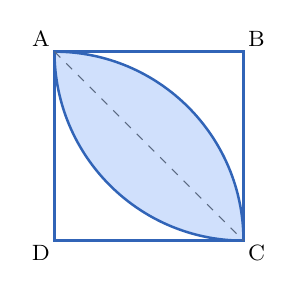
\begin{tikzpicture}[scale=0.24]
\fill[shade] (10,0) arc (0:90:10) arc (180:270:10);
\draw[geo] (0,0) rectangle (10,10);
\draw[geo] (10,0) arc (0:90:10); \draw[geo] (0,10) arc (180:270:10);
\draw[dashed,Slate] (0,10)--(10,0);
\node[lbl,below left] at (0,0){D}; \node[lbl,below right] at (10,0){C}; \node[lbl,above right] at (10,10){B}; \node[lbl,above left] at (0,10){A};
\end{tikzpicture}
\end{minipage}
\end{probbox}
\probsol{
Diagonal AC splits the leaf into two equal halves.\par Each half is a quarter circle minus a right-angled triangle:\par
$10\times10\times3.14:4-10\times10:2=78.5-50=28.5$ cm$^2$.\par
Leaf: $28.5\times2=57$ cm$^2$.
\dapso{$57$ cm$^2$.}}
\gap
\begin{probbox}{37}{\stars{1}}
Two circles with the same centre have radii $4$ m and $6$ m. Find the area of the ring between them.
\end{probbox}
\probsol{
Large circle: $6\times6\times3.14=113.04$ m$^2$.\par Small circle: $4\times4\times3.14=50.24$ m$^2$.\par Required area: $113.04-50.24=62.8$ m$^2$.
\dapso{$62.8$ m$^2$.}}
\gap
\begin{probbox}{38}{\stars{1}}
A round flower bed has radius $8$ m, with a path $2$ m wide around it. Find the area of the path.
\end{probbox}
\probsol{
Large circle: $10\times10\times3.14=314$ m$^2$.\par Small circle: $8\times8\times3.14=200.96$ m$^2$.\par Required area: $314-200.96=113.04$ m$^2$.
\dapso{$113.04$ m$^2$.}}
\gap
\begin{probbox}{39}{\stars{1}}
A square has its four corners on a circle of radius $6$ cm. Find the area of the circle outside the square.
\end{probbox}
\probsol{
The square's diagonals are diameters, $12$ cm long and perpendicular.\par It is $4$ right triangles with legs $6$ cm: $6\times6:2\times4=72$ cm$^2$.\par Circle: $6\times6\times3.14=113.04$ cm$^2$.\par Required: $113.04-72=41.04$ cm$^2$.
\dapso{$41.04$ cm$^2$.}}
\gap
\begin{probbox}{40}{\stars{1}}
A small wheel of radius $0.3$ m makes $150$ turns. A large wheel covers the same distance in $90$ turns. Find its radius.
\end{probbox}
\probsol{
Distance: $0.3\times2\times3.14\times150=282.6$ m.\par One large turn: $282.6:90=3.14$ m.\par Radius: $3.14:3.14:2=0.5$ m.
\dapso{$0.5$ m.}}
\gap
\begin{probbox}{41}{\stars{1}}
A circle has the same perimeter as a square of side $15.7$ cm. Which has the larger area, and by how much?
\end{probbox}
\probsol{
Square perimeter: $62.8$ cm.\par Circle radius: $62.8:3.14:2=10$ cm; area $314$ cm$^2$.\par Square area: $15.7\times15.7=246.49$ cm$^2$.\par The circle is larger by $67.51$ cm$^2$.
\dapso{The circle, by $67.51$ cm$^2$.}}
\gap
\begin{probbox}{42}{\stars{1}}
A circle has area $12.56$ cm$^2$. If its radius is doubled, what is the new area?
\end{probbox}
\probsol{
Doubling $r$ multiplies $r\times r$ by $2\times2=4$.\par New area: $12.56\times4=50.24$ cm$^2$.
\dapso{$50.24$ cm$^2$.}}
\gap
\begin{probbox}{43}{\stars{1}}
A circle's radius grows by $1.5$ cm. By how much does its circumference grow?
\end{probbox}
\probsol{
$C=r\times2\times3.14$, so $C$ grows by $1.5\times2\times3.14=9.42$ cm.\par This does not depend on the original radius.
\dapso{$9.42$ cm.}}
\gap
\begin{probbox}{44}{\stars{1}}
An old bicycle has a front wheel of diameter $0.5$ m and a back wheel of diameter $1$ m. When the back wheel turns $100$ times, how many times does the front wheel turn?
\end{probbox}
\probsol{
Distance: $1\times3.14\times100=314$ m.\par One front turn: $0.5\times3.14=1.57$ m.\par Front turns: $314:1.57=200$.
\dapso{$200$ turns.}}
\gap
\begin{probbox}{45}{\stars{1}}
A running track has two straights of $100$ m and two semicircular ends of diameter $60$ m. Find the length of one lap and the area inside.
\end{probbox}
\probsol{
Two semicircles make one circle: $60\times3.14=188.4$ m.\par One lap: $100\times2+188.4=388.4$ m.\par Rectangle: $6\,000$ m$^2$; circle: $30\times30\times3.14=2\,826$ m$^2$.\par Inside area: $8\,826$ m$^2$.
\dapso{$388.4$ m; $8\,826$ m$^2$.}}
\gap
\begin{probbox}{46}{\stars{2}}
A quarter (bounded by two perpendicular radii) is cut from a circular card of radius $10$ cm. Find the area and perimeter of what is left.
\end{probbox}
\probsol{
Circle: $314$ cm$^2$; three quarters: $235.5$ cm$^2$.\par Circumference $62.8$ cm; the remaining arc: $47.1$ cm.\par Perimeter: arc plus two radii, $47.1+20=67.1$ cm.
\dapso{$235.5$ cm$^2$; $67.1$ cm.}}
\gap
\begin{probbox}{47}{\stars{2}}
A goat is tied to an outside corner of a square pen of side $6$ m with a $4$ m rope. It cannot enter the pen. Find the area it can graze.
\end{probbox}
\probsol{
The rope is shorter than the side, so the goat only swings round that corner.\par The pen blocks $\dfrac14$ of the circle, leaving $\dfrac34$ of a circle of radius $4$ m.\par Area: $4\times4\times3.14\times\dfrac34=37.68$ m$^2$.
\dapso{$37.68$ m$^2$.}}
\gap
\begin{probbox}{48}{\stars{1}}
Two circles' circumferences differ by $12.56$ cm, and the larger radius is $3$ times the smaller. Find the area of the larger circle.
\end{probbox}
\probsol{
Difference of radii: $12.56:2:3.14=2$ cm.\par $3-1=2$ parts make $2$ cm, so the radii are $1$ cm and $3$ cm.\par Larger area: $3\times3\times3.14=28.26$ cm$^2$.
\dapso{$28.26$ cm$^2$.}}
\gap
\begin{probbox}{49}{\stars{1}}
A minute hand is $12$ cm long. What area does it sweep in $20$ minutes?
\end{probbox}
\probsol{
$20$ minutes is $\dfrac13$ of a turn.\par Circle: $12\times12\times3.14=452.16$ cm$^2$.\par Swept area: $452.16:3=150.72$ cm$^2$.
\dapso{$150.72$ cm$^2$.}}
\gap
\begin{probbox}{50}{\stars{1}}
A tractor wheel of diameter $0.7$ m makes $120$ turns a minute. How far does the tractor go in $10$ minutes?
\end{probbox}
\probsol{
One turn: $0.7\times3.14=2.198$ m.\par Turns in $10$ minutes: $1\,200$.\par Distance: $2.198\times1\,200=2\,637.6$ m.
\dapso{$2\,637.6$ m.}}
\clearpage
\titlehead
\begingroup\setbox0=\vbox{\section*{Mixed Practice on Area}}\endgroup
\chapterhead{15}{Mixed Practice on Area}

\shead{Split, add on, cut away}
\begin{knowbox}
To find the area of a composite shape, reduce it to shapes whose formulas we know:
\begin{center}\renewcommand{\arraystretch}{1.5}
\begin{tabular}{|l|c||l|c|}\hline
Rectangle & $a\times b$ & Triangle & $a\times h:2$\\\hline
Square & $a\times a$ & Trapezium & $(a+b)\times h:2$\\\hline
Circle & $r\times r\times3.14$ & Semicircle & $r\times r\times3.14:2$\\\hline
\end{tabular}\end{center}
\begin{itemize}[leftmargin=1.4em,itemsep=3pt]
\item \textbf{Split:} cut the shape into familiar pieces and \emph{add} their areas.
\item \textbf{Complete and subtract:} fill it out to a large familiar shape and \emph{subtract} what was added.
\item Always change measurements to \textbf{the same unit} first; $1$ m$^2=100$ dm$^2=10\,000$ cm$^2$.
\end{itemize}
\end{knowbox}
\gap
\begin{exbox}{\ExWord\ 1}
\begin{minipage}[t]{0.62\linewidth}
A plot of land is shaped as shown: a rectangle $20$ m by $12$ m with a triangle on top whose base is the rectangle's length and whose height is $8$ m. Find the area of the plot.
\end{minipage}\hfill
\begin{minipage}[t]{0.34\linewidth}\vspace{0pt}\centering
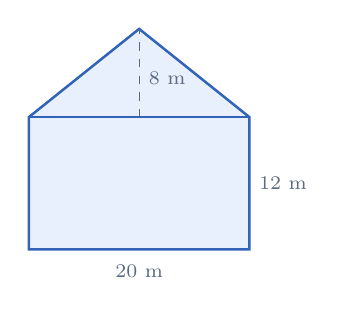
\begin{tikzpicture}[scale=0.14]
\fill[tmBlue!12] (0,0)--(20,0)--(20,12)--(10,20)--(0,12)--cycle;
\draw[geo] (0,0)--(20,0)--(20,12)--(10,20)--(0,12)--cycle; \draw[geo] (0,12)--(20,12);
\draw[dashed,Slate] (10,12)--(10,20);
\node[dim] at (10,-2){$20$ m}; \node[dim,right] at (20,6){$12$ m}; \node[dim,right] at (10,15.5){$8$ m};
\end{tikzpicture}
\end{minipage}
\guide
\textbf{Split} it into a rectangle and a triangle:\par
$S_\text{rectangle}=20\times12=240$ m$^2$;\par $S_\text{triangle}=20\times8:2=80$ m$^2$.\par Plot: $240+80=320$ m$^2$.
\dapso{$320$ m$^2$.}
\end{exbox}
\gap
\begin{exbox}{\ExWord\ 2}
\begin{minipage}[t]{0.62\linewidth}
A semicircle whose diameter is the width of a $16$ cm by $10$ cm wooden board is cut out of it (see the figure). Find the area of the wood that is left.
\end{minipage}\hfill
\begin{minipage}[t]{0.34\linewidth}\vspace{0pt}\centering
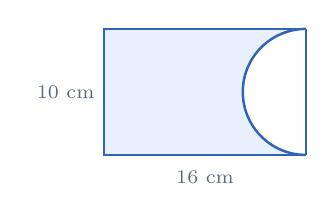
\begin{tikzpicture}[scale=0.16]
\fill[tmBlue!12] (0,0)--(16,0)--(16,10)--(0,10)--cycle; \fill[white] (16,0) arc (-90:-270:5);
\draw[geo] (16,0)--(0,0)--(0,10)--(16,10); \draw[geo] (16,10)--(16,0); \draw[geo] (16,0) arc (-90:-270:5);
\node[dim] at (8,-1.8){$16$ cm}; \node[dim,left] at (0,5){$10$ cm};
\end{tikzpicture}
\end{minipage}
\guide
$S_\text{board}=16\times10=160$ cm$^2$.\par The semicircle has $r=5$ cm: $5\times5\times3.14:2=39.25$ cm$^2$.\par
Wood left: $160-39.25=120.75$ cm$^2$.
\dapso{$120.75$ cm$^2$.}
\end{exbox}
\gap
\begin{exbox}{\ExWord\ 3}
On a map with scale $1:1\,000$, a trapezium-shaped garden has bases $5$ cm and $3$ cm and height $4$ cm. Find the real area of the garden.
\guide
Real lengths: $5$ cm $\to5\,000$ cm $=50$ m;\par $3$ cm $\to30$ m;\par $4$ cm $\to40$ m.\par
Real area: $(50+30)\times40:2=1\,600$ m$^2$.\par
\emph{Note:} change to real lengths \emph{first}, then compute the area.
\dapso{$1\,600$ m$^2$.}
\end{exbox}
\gap
\begin{exbox}{\ExWord\ 4}
A rectangular floor is $8$ m by $6$ m. It is tiled with square tiles of side $40$ cm costing $25\,000$ dong each. How many tiles are needed, and what do they cost? (Ignore the grout.)
\guide
Floor: $8\times6=48$ m$^2$ $=480\,000$ cm$^2$.\par One tile: $40\times40=1\,600$ cm$^2$.\par
Tiles: $480\,000:1\,600=300$.\par Cost: $25\,000\times300=7\,500\,000$ dong.
\dapso{$300$ tiles; $7\,500\,000$ dong.}
\end{exbox}
\dividerbar{Practice}
\begin{probbox}{1}{\relax}
\begin{minipage}[t]{0.66\linewidth}
Find the area of the L-shape (measurements in centimetres).
\end{minipage}\hfill
\begin{minipage}[t]{0.3\linewidth}\vspace{0pt}\centering
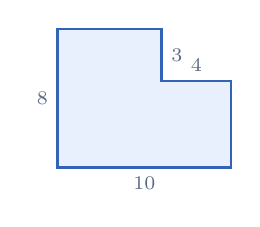
\begin{tikzpicture}[scale=0.22]
\fill[tmBlue!12] (0,0)--(10,0)--(10,5)--(6,5)--(6,8)--(0,8)--cycle;
\draw[geo] (0,0)--(10,0)--(10,5)--(6,5)--(6,8)--(0,8)--cycle;
\node[dim,below] at (5,0){$10$}; \node[dim,left] at (0,4){$8$}; \node[dim,above] at (8,5){$4$}; \node[dim,right] at (6,6.5){$3$};
\end{tikzpicture}
\end{minipage}
\end{probbox}
\probsol{
\emph{Complete and subtract:} $10\times8-4\times3=80-12=68$ cm$^2$.
\dapso{$68$ cm$^2$.}}
\gap
\begin{probbox}{2}{\relax}
A rectangular plot is $25$ m long, and its width is $\dfrac35$ of its length. A house with a square base of side $10$ m is built on it. Find the area left.
\end{probbox}
\probsol{
Width: $25\times\dfrac35=15$ m.\par Left: $25\times15-10\times10=375-100=275$ m$^2$.
\dapso{$275$ m$^2$.}}
\gap
\begin{probbox}{3}{\relax}
A rectangular schoolyard is $50$ m by $30$ m. A round flower bed of radius $3$ m is in the middle. Find the rest of the yard's area.
\end{probbox}
\probsol{
$50\times30-3\times3\times3.14=1\,500-28.26=1\,471.74$ m$^2$.
\dapso{$1\,471.74$ m$^2$.}}
\gap
\begin{probbox}{4}{\relax}
A trapezium-shaped garden has bases $30$ m and $20$ m and height $16$ m. A quarter of it is dug out for a pond and the rest is planted. Find the planted area.
\end{probbox}
\probsol{
$S=(30+20)\times16:2=400$ m$^2$.\par Planted: $400\times\dfrac34=300$ m$^2$.
\dapso{$300$ m$^2$.}}
\gap
\begin{probbox}{5}{\relax}
On a $1:500$ map a rectangular pitch is $6$ cm by $4$ cm. Find its real area.
\end{probbox}
\probsol{
Real size: $6\times500=3\,000$ cm $=30$ m;\par $4\times500=2\,000$ cm $=20$ m.\par Area: $30\times20=600$ m$^2$.
\dapso{$600$ m$^2$.}}
\gap
\begin{probbox}{6}{\relax}
A classroom $6$ m by $4$ m is tiled with square tiles of side $50$ cm. How many tiles are needed?
\end{probbox}
\probsol{
Room: $24$ m$^2$ $=240\,000$ cm$^2$; one tile: $2\,500$ cm$^2$.\par Tiles: $240\,000:2\,500=96$.
\dapso{$96$ tiles.}}
\gap
\begin{probbox}{7}{\relax}
Four equal squares of side $0.2$ m are cut from the corners of a $2$ m by $1.5$ m metal sheet. Find the area of metal left.
\end{probbox}
\probsol{
$2\times1.5-4\times0.2\times0.2=3-0.16=2.84$ m$^2$.
\dapso{$2.84$ m$^2$.}}
\gap
\begin{probbox}{8}{\relax}
A shape is made of a square of side $6$ cm and a semicircle drawn outwards on one side of the square. Find its area and perimeter.
\end{probbox}
\probsol{
Area: $6\times6+3\times3\times3.14:2=36+14.13=50.13$ cm$^2$.\par
The perimeter is three sides of the square plus the half circle: $6\times3+6\times3.14:2=18+9.42=27.42$ cm.
\dapso{$50.13$ cm$^2$; $27.42$ cm.}}
\gap
\begin{probbox}{9}{\relax}
The diagonals of rectangle ABCD ($AB=12$ cm, $BC=8$ cm) cross at O. Show that triangles OAB, OBC, OCD and ODA have equal areas, and find each area.
\end{probbox}
\probsol{
O is the midpoint of each diagonal.\par In triangle ABC, BO joins B to the midpoint of AC, so $S_{OAB}=S_{OBC}$; likewise $S_{OBC}=S_{OCD}$ and $S_{OCD}=S_{ODA}$.\par
Each triangle: $12\times8:4=24$ cm$^2$.
\dapso{$24$ cm$^2$.}}
\gap
\begin{probbox}{10}{\relax}
On a map at scale $1:1\,000$, a rectangular plot is $6$ cm by $4$ cm. Find its real area.
\end{probbox}
\probsol{
Real length: $6\times1\,000=6\,000$ cm $=60$ m.\par Real width: $4\times1\,000=4\,000$ cm $=40$ m.\par Area: $60\times40=2\,400$ m$^2$.
\dapso{$2\,400$ m$^2$.}}
\gap
\begin{probbox}{11}{\relax}
On a map at scale $1:2\,000$, a rectangular plot is $5$ cm by $3$ cm. Find its real area.
\end{probbox}
\probsol{
Real length: $5\times2\,000=10\,000$ cm $=100$ m.\par Real width: $3\times2\,000=6\,000$ cm $=60$ m.\par Area: $100\times60=6\,000$ m$^2$.
\dapso{$6\,000$ m$^2$.}}
\gap
\begin{probbox}{12}{\relax}
On a map at scale $1:500$, a rectangular plot is $8$ cm by $5$ cm. Find its real area.
\end{probbox}
\probsol{
Real length: $8\times500=4\,000$ cm $=40$ m.\par Real width: $5\times500=2\,500$ cm $=25$ m.\par Area: $40\times25=1\,000$ m$^2$.
\dapso{$1\,000$ m$^2$.}}
\gap
\begin{probbox}{13}{\relax}
A room floor is $6$ m by $4$ m, tiled with square tiles of side $40$ cm costing $20\,000$ dong each. Find the number of tiles and their cost (ignore the joints).
\end{probbox}
\probsol{
Floor: $6\times4=24$ m$^2$.\par One tile: $40\times40=1600$ cm$^2$ $=0.16$ m$^2$.\par Tiles: $24:0.16=150$.\par Cost: $20\,000\times150=3\,000\,000$ dong.
\dapso{$150$ tiles; $3\,000\,000$ dong.}}
\gap
\begin{probbox}{14}{\relax}
A room floor is $8$ m by $5$ m, tiled with square tiles of side $50$ cm costing $35\,000$ dong each. Find the number of tiles and their cost (ignore the joints).
\end{probbox}
\probsol{
Floor: $8\times5=40$ m$^2$.\par One tile: $50\times50=2500$ cm$^2$ $=0.25$ m$^2$.\par Tiles: $40:0.25=160$.\par Cost: $35\,000\times160=5\,600\,000$ dong.
\dapso{$160$ tiles; $5\,600\,000$ dong.}}
\gap
\begin{probbox}{15}{\relax}
A room floor is $4.8$ m by $3.6$ m, tiled with square tiles of side $60$ cm costing $45\,000$ dong each. Find the number of tiles and their cost (ignore the joints).
\end{probbox}
\probsol{
Floor: $4.8\times3.6=17.28$ m$^2$.\par One tile: $60\times60=3600$ cm$^2$ $=0.36$ m$^2$.\par Tiles: $17.28:0.36=48$.\par Cost: $45\,000\times48=2\,160\,000$ dong.
\dapso{$48$ tiles; $2\,160\,000$ dong.}}
\gap
\begin{probbox}{16}{\relax}
A rectangular plot is $30$ m long and its width is $\dfrac{2}{3}$ of the length. A $12$ m $\times$ $8$ m house is built on it. Find the remaining area.
\end{probbox}
\probsol{
Width: $30\times\dfrac{2}{3}=20$ m.\par Plot: $600$ m$^2$.\par House: $96$ m$^2$.\par Remaining: $504$ m$^2$.
\dapso{$504$ m$^2$.}}
\gap
\begin{probbox}{17}{\relax}
A rectangular plot is $40$ m long and its width is $\dfrac{3}{4}$ of the length. A $15$ m $\times$ $10$ m house is built on it. Find the remaining area.
\end{probbox}
\probsol{
Width: $40\times\dfrac{3}{4}=30$ m.\par Plot: $1\,200$ m$^2$.\par House: $150$ m$^2$.\par Remaining: $1\,050$ m$^2$.
\dapso{$1\,050$ m$^2$.}}
\gap
\begin{probbox}{18}{\relax}
A playground is $40$ m by $25$ m with a round sandpit of radius $3$ m in the middle. Find the area of the rest.
\end{probbox}
\probsol{
Playground: $1000$ m$^2$.\par Sandpit: $3\times3\times3.14=28.26$ m$^2$.\par Rest: $971.74$ m$^2$.
\dapso{$971.74$ m$^2$.}}
\gap
\begin{probbox}{19}{\relax}
A playground is $30$ m by $20$ m with a round sandpit of radius $5$ m in the middle. Find the area of the rest.
\end{probbox}
\probsol{
Playground: $600$ m$^2$.\par Sandpit: $5\times5\times3.14=78.5$ m$^2$.\par Rest: $521.5$ m$^2$.
\dapso{$521.5$ m$^2$.}}
\gap
\begin{probbox}{20}{\relax}
A shape is a square of side $8$ cm with a semicircle on one side (diameter $=$ that side), outward. Find its area.
\end{probbox}
\probsol{
Square: $64$ cm$^2$.\par Semicircle of radius $4$ cm: $25.12$ cm$^2$.\par Total: $89.12$ cm$^2$.
\dapso{$89.12$ cm$^2$.}}
\gap
\begin{probbox}{21}{\relax}
A shape is a square of side $10$ cm with a semicircle on one side (diameter $=$ that side), outward. Find its area.
\end{probbox}
\probsol{
Square: $100$ cm$^2$.\par Semicircle of radius $5$ cm: $39.25$ cm$^2$.\par Total: $139.25$ cm$^2$.
\dapso{$139.25$ cm$^2$.}}
\gap
\begin{probbox}{22}{\relax}
From a $3$ dm $\times$ $2$ dm card, a square of side $0.4$ dm is cut from each corner. Find the area left.
\end{probbox}
\probsol{
Card: $6$ dm$^2$.\par Four squares: $0.64$ dm$^2$.\par Left: $5.36$ dm$^2$.
\dapso{$5.36$ dm$^2$.}}
\gap
\begin{probbox}{23}{\relax}
From a $5$ dm $\times$ $4$ dm card, a square of side $0.5$ dm is cut from each corner. Find the area left.
\end{probbox}
\probsol{
Card: $20$ dm$^2$.\par Four squares: $1$ dm$^2$.\par Left: $19$ dm$^2$.
\dapso{$19$ dm$^2$.}}
\gap
\begin{probbox}{24}{\relax}
A trapezium-shaped garden has bases $40$ m and $30$ m and height $20$ m. $\dfrac{1}{5}$ of it is a pond; vegetables grow on the rest at $3$ kg per m$^2$. Find the harvest.
\end{probbox}
\probsol{
Garden: $700$ m$^2$.\par Pond: $140$ m$^2$.\par Vegetables: $560$ m$^2$.\par Harvest: $560\times3=1\,680$ kg.
\dapso{$1\,680$ kg.}}
\gap
\begin{probbox}{25}{\relax}
A trapezium-shaped garden has bases $60$ m and $40$ m and height $30$ m. $\dfrac{1}{3}$ of it is a pond; vegetables grow on the rest at $2$ kg per m$^2$. Find the harvest.
\end{probbox}
\probsol{
Garden: $1\,500$ m$^2$.\par Pond: $500$ m$^2$.\par Vegetables: $1\,000$ m$^2$.\par Harvest: $1\,000\times2=2\,000$ kg.
\dapso{$2\,000$ kg.}}
\gap
\begin{probbox}{26}{\relax}
An L-shaped plot is a $20$ m $\times$ $15$ m rectangle with a $8$ m $\times$ $6$ m corner removed. Find its area.
\end{probbox}
\probsol{
Big rectangle: $300$ m$^2$.\par Cut-out: $48$ m$^2$.\par Area: $252$ m$^2$.
\dapso{$252$ m$^2$.}}
\gap
\begin{probbox}{27}{\relax}
An L-shaped plot is a $30$ m $\times$ $24$ m rectangle with a $12$ m $\times$ $10$ m corner removed. Find its area.
\end{probbox}
\probsol{
Big rectangle: $720$ m$^2$.\par Cut-out: $120$ m$^2$.\par Area: $600$ m$^2$.
\dapso{$600$ m$^2$.}}
\gap
\begin{probbox}{28}{\relax}
A rectangular garden has perimeter $60$ m, and its width is $\dfrac{2}{3}$ of its length. Find its area.
\end{probbox}
\probsol{
Half perimeter: $30$ m.\par $5$ parts; one part: $6$ m.\par Length $18$ m, width $12$ m.\par Area: $216$ m$^2$.
\dapso{$216$ m$^2$.}}
\gap
\begin{probbox}{29}{\relax}
A rectangular garden has perimeter $84$ m, and its width is $\dfrac{3}{4}$ of its length. Find its area.
\end{probbox}
\probsol{
Half perimeter: $42$ m.\par $7$ parts; one part: $6$ m.\par Length $24$ m, width $18$ m.\par Area: $432$ m$^2$.
\dapso{$432$ m$^2$.}}
\gap
\begin{probbox}{30}{\relax}
A rectangular garden has perimeter $100$ m, and its width is $\dfrac{1}{4}$ of its length. Find its area.
\end{probbox}
\probsol{
Half perimeter: $50$ m.\par $5$ parts; one part: $10$ m.\par Length $40$ m, width $10$ m.\par Area: $400$ m$^2$.
\dapso{$400$ m$^2$.}}
\dividerbar{Challenge -- Extension}
\begin{probbox}{31}{\stars{1}}
A rectangular garden has perimeter $56$ m. Adding $4$ m to its width and taking $4$ m from its length makes it a square. Find its area.
\end{probbox}
\probsol{
The length is $4+4=8$ m more than the width; half the perimeter is $28$ m.\par Length: $(28+8):2=18$ m; width: $10$ m.\par Area: $180$ m$^2$.
\dapso{$180$ m$^2$.}}
\gap
\begin{probbox}{32}{\stars{1}}
Adding $5$ m to the length of a rectangular garden adds $60$ m$^2$; taking $3$ m from its width removes $75$ m$^2$. Find its area.
\end{probbox}
\probsol{
The added strip is $5$ m by the width, so the width is $60:5=12$ m.\par The removed strip is $3$ m by the length, so the length is $75:3=25$ m.\par
Area: $25\times12=300$ m$^2$.
\dapso{$300$ m$^2$.}}
\gap
\begin{probbox}{33}{\stars{1}}
\begin{minipage}[t]{0.62\linewidth}
A $40$ m by $25$ m vegetable garden has two paths $2$ m wide crossing at right angles, running the full length and width (see the figure). Find the planted area.
\end{minipage}\hfill
\begin{minipage}[t]{0.34\linewidth}\vspace{0pt}\centering
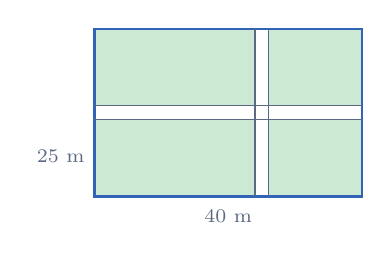
\begin{tikzpicture}[scale=0.085]
\fill[tmGreen!25] (0,0) rectangle (40,25);
\fill[white] (0,11.5) rectangle (40,13.5); \fill[white] (24,0) rectangle (26,25);
\draw[geo] (0,0) rectangle (40,25);
\draw[Slate] (0,11.5)--(40,11.5) (0,13.5)--(40,13.5) (24,0)--(24,25) (26,0)--(26,25);
\node[dim] at (20,-3){$40$ m}; \node[dim,left] at (0,6){$25$ m};
\end{tikzpicture}
\end{minipage}
\end{probbox}
\probsol{
Pushing the planted pieces together gives a rectangle $40-2=38$ m long and $25-2=23$ m wide.\par
Planted area: $38\times23=874$ m$^2$.
\dapso{$874$ m$^2$.}}
\gap
\begin{probbox}{34}{\stars{1}}
The two largest possible non-overlapping circles are cut from a $20$ cm by $10$ cm card. Find the area of card left over.
\end{probbox}
\probsol{
Each circle has diameter $10$ cm ($r=5$ cm), and two fit side by side along the $20$ cm length.\par
Left over: $20\times10-2\times5\times5\times3.14=200-157=43$ cm$^2$.
\dapso{$43$ cm$^2$.}}
\gap
\begin{probbox}{35}{\stars{2}}
Triangle ABC has a right angle at A, $AB=12$ cm, $AC=16$ cm and $BC=20$ cm. Semicircles are drawn outwards on AB, AC and BC. Show that the semicircle on BC has the same area as the other two together.
\end{probbox}
\probsol{
Semicircle on AB ($r=6$): $6\times6\times3.14:2=56.52$ cm$^2$.\par
Semicircle on AC ($r=8$): $8\times8\times3.14:2=100.48$ cm$^2$.\par
Semicircle on BC ($r=10$): $10\times10\times3.14:2=157$ cm$^2$ $=56.52+100.48$.
\dapso{$157=56.52+100.48$ (cm$^2$).}}
\gap
\begin{probbox}{36}{\stars{1}}
A rectangular garden has perimeter $64$ m. Adding $5$ m to the width and taking $5$ m off the length makes it a square. Find its area.
\end{probbox}
\probsol{
Then length and width are equal, so the length is $5+5=10$ m longer.\par Half perimeter: $32$ m.\par Length: $(32+10):2=21$ m; width: $11$ m.\par Area: $231$ m$^2$.
\dapso{$231$ m$^2$.}}
\gap
\begin{probbox}{37}{\stars{1}}
A rectangular garden has perimeter $80$ m. Adding $3$ m to the width and taking $3$ m off the length makes it a square. Find its area.
\end{probbox}
\probsol{
Then length and width are equal, so the length is $3+3=6$ m longer.\par Half perimeter: $40$ m.\par Length: $(40+6):2=23$ m; width: $17$ m.\par Area: $391$ m$^2$.
\dapso{$391$ m$^2$.}}
\gap
\begin{probbox}{38}{\stars{1}}
For a rectangular garden, adding $6$ m to the length adds $84$ m$^2$; taking $4$ m off the width removes $72$ m$^2$. Find its area.
\end{probbox}
\probsol{
The added strip is $6$ m by the width, so width $=84:6=14$ m.\par The removed strip is $4$ m by the length, so length $=72:4=18$ m.\par Area: $18\times14=252$ m$^2$.
\dapso{$252$ m$^2$.}}
\gap
\begin{probbox}{39}{\stars{1}}
For a rectangular garden, adding $4$ m to the length adds $40$ m$^2$; taking $2$ m off the width removes $48$ m$^2$. Find its area.
\end{probbox}
\probsol{
The added strip is $4$ m by the width, so width $=40:4=10$ m.\par The removed strip is $2$ m by the length, so length $=48:2=24$ m.\par Area: $24\times10=240$ m$^2$.
\dapso{$240$ m$^2$.}}
\gap
\begin{probbox}{40}{\stars{1}}
A garden is $30$ m by $20$ m. Two paths $2$ m wide cross it, one parallel to each side. Find the area left for planting.
\end{probbox}
\probsol{
Long path: $60$ m$^2$; short path: $40$ m$^2$.\par The $2\times2=4$ m$^2$ crossing is counted twice.\par Paths: $60+40-4=96$ m$^2$.\par Left: $600-96=504$ m$^2$.
\dapso{$504$ m$^2$.}}
\gap
\begin{probbox}{41}{\stars{1}}
A garden is $45$ m by $32$ m. Two paths $3$ m wide cross it, one parallel to each side. Find the area left for planting.
\end{probbox}
\probsol{
Long path: $135$ m$^2$; short path: $96$ m$^2$.\par The $3\times3=9$ m$^2$ crossing is counted twice.\par Paths: $135+96-9=222$ m$^2$.\par Left: $1440-222=1\,218$ m$^2$.
\dapso{$1\,218$ m$^2$.}}
\gap
\begin{probbox}{42}{\stars{1}}
A $25$ m by $10$ m pool has a paved strip $2$ m wide all round. Find the area of the strip.
\end{probbox}
\probsol{
Outer size: $29$ m by $14$ m.\par Outer area: $406$ m$^2$.\par Pool: $250$ m$^2$.\par Strip: $156$ m$^2$.
\dapso{$156$ m$^2$.}}
\gap
\begin{probbox}{43}{\stars{2}}
Rectangle ABCD has $AB=12$ cm, $BC=8$ cm. A semicircle on AB is drawn inside it. Find the area of the rectangle outside the semicircle.
\end{probbox}
\probsol{
Radius $6$ cm $<8$ cm, so the semicircle fits inside.\par Semicircle: $6\times6\times3.14:2=56.52$ cm$^2$.\par Rectangle: $96$ cm$^2$.\par Required: $96-56.52=39.48$ cm$^2$.
\dapso{$39.48$ cm$^2$.}}
\gap
\begin{probbox}{44}{\stars{1}}
Square ABCD has side $10$ cm. Joining the midpoints of its sides gives square MNPQ. Find its area.
\end{probbox}
\probsol{
Each corner is a right triangle with legs $5$ cm: $12.5$ cm$^2$.\par Four of them: $50$ cm$^2$.\par $S_{MNPQ}=100-50=50$ cm$^2$, half the original.
\dapso{$50$ cm$^2$.}}
\gap
\begin{probbox}{45}{\stars{1}}
A rectangle is cut into four smaller rectangles by one line parallel to each side. Three have areas $12$, $18$ and $20$ cm$^2$ ($12$ and $18$ side by side on top, $20$ below the $12$). Find the fourth.
\end{probbox}
\probsol{
The top two share a height, so their widths are in the ratio $12:18=\dfrac23$.\par The bottom two share a height and have the same widths.\par So the fourth is $20:\dfrac23=30$ cm$^2$.
\dapso{$30$ cm$^2$.}}
\gap
\begin{probbox}{46}{\stars{1}}
A $40$ cm by $30$ cm picture has a frame $5$ cm wide all round. Find the area of the frame.
\end{probbox}
\probsol{
Outer size: $50$ cm by $40$ cm.\par Outer area: $2\,000$ cm$^2$.\par Picture: $1\,200$ cm$^2$.\par Frame: $800$ cm$^2$.
\dapso{$800$ cm$^2$.}}
\gap
\begin{probbox}{47}{\stars{1}}
A \emph{flower} shape is a square of side $4$ cm with four outward semicircles on its sides. Find its area.
\end{probbox}
\probsol{
Square: $16$ cm$^2$.\par Each semicircle (radius $2$ cm): $6.28$ cm$^2$.\par Four: $25.12$ cm$^2$.\par Flower: $41.12$ cm$^2$.
\dapso{$41.12$ cm$^2$.}}
\gap
\begin{probbox}{48}{\stars{1}}
A plot has a real area of $4\,800$ m$^2$. What is its area in cm$^2$ on a $1:2\,000$ map?
\end{probbox}
\probsol{
Lengths shrink $2\,000$ times, so areas shrink $2\,000\times2\,000=4\,000\,000$ times.\par $4\,800$ m$^2$ $=48\,000\,000$ cm$^2$.\par On the map: $12$ cm$^2$.
\dapso{$12$ cm$^2$.}}
\gap
\begin{probbox}{49}{\stars{1}}
A rectangular garden has perimeter $120$ m and its length is twice its width. Vegetables grow on $\dfrac34$ of it at $2$ kg per m$^2$. How much is harvested?
\end{probbox}
\probsol{
Half perimeter $60$ m; width $60:3=20$ m; length $40$ m.\par Area: $800$ m$^2$.\par Vegetables: $800\times\dfrac34=600$ m$^2$.\par Harvest: $1\,200$ kg.
\dapso{$1\,200$ kg.}}
\gap
\begin{probbox}{50}{\stars{2}}
A right-trapezium field has bases $50$ m and $30$ m. Extending the shorter base by $20$ m turns it into a rectangle and adds $400$ m$^2$. Find the original area.
\end{probbox}
\probsol{
The added part is a right triangle with legs $20$ m and the height.\par Height: $400\times2:20=40$ m.\par Original area: $(50+30)\times40:2=1\,600$ m$^2$.
\dapso{$1\,600$ m$^2$.}}
\clearpage
\begingroup\setbox0=\vbox{\section*{Mixed Review -- Paper 1}}\endgroup\renewcommand{\CurTopic}{Mixed Review -- Paper 1}\setcounter{seccnt}{0}\phantomsection\pdfbookmark[0]{Mixed Review -- Paper 1}{rev1}\label{toc:rev1}\par\vspace{0.1cm}\noindent
\begin{tikzpicture}[baseline=-0.5ex]\node[circle,fill=tmOrange,text=white,font=\large\bfseries,minimum size=0.95cm,inner sep=0pt](cn){\faPen};\node[anchor=west,font=\LARGE\bfseries,text=tmOrange] at ([xshift=12pt]cn.east){Mixed Review -- Paper 1};\end{tikzpicture}\par\vspace{4pt}\noindent\textcolor{tmOrange}{\rule{\linewidth}{2pt}}\par\vspace{0.5cm}

\begin{knowbox}
\textbf{Covers:} Chapters 1 -- 8 (whole numbers, fractions, decimals, standard word problems, proportion, work problems). \quad \textbf{Suggested time:} $60$ minutes.
\end{knowbox}
\gap
\begin{probbox}{1}{\relax}
Consider $4,\ 7,\ 10,\ \ldots,\ 301$. \ \pa{a} How many terms are there? \ \pa{b} Find their sum.
\end{probbox}
\probsol{
\pa{a} $(301-4):3+1=100$ terms.\par \pa{b} $(4+301)\times100:2=15\,250$.
\dapso{$100$; $15\,250$.}}
\gap
\begin{probbox}{2}{\relax}
Calculate cleverly: $25\times37\times4+63\times100$.
\end{probbox}
\probsol{
$=37\times100+63\times100=(37+63)\times100=10\,000$.
\dapso{$10\,000$.}}
\gap
\begin{probbox}{3}{\relax}
Compare $\dfrac79$ and $\dfrac9{11}$ without finding a common denominator.
\end{probbox}
\probsol{
$1-\dfrac79=\dfrac29$ and $1-\dfrac9{11}=\dfrac2{11}$.\par Since $\dfrac29>\dfrac2{11}$, $\dfrac79<\dfrac9{11}$.
\dapso{$\dfrac79<\dfrac9{11}$.}}
\gap
\begin{probbox}{4}{\relax}
Calculate: $\dfrac12+\dfrac16+\dfrac1{12}+\dfrac1{20}+\dfrac1{30}$.
\end{probbox}
\probsol{
$=\left(1-\dfrac12\right)+\left(\dfrac12-\dfrac13\right)+\cdots+\left(\dfrac15-\dfrac16\right)=1-\dfrac16=\dfrac56$.
\dapso{$\dfrac56$.}}
\gap
\begin{probbox}{5}{\relax}
Calculate: $2\dfrac34+1\dfrac56$.
\end{probbox}
\probsol{
$=\dfrac{11}4+\dfrac{11}6=\dfrac{33}{12}+\dfrac{22}{12}=\dfrac{55}{12}=4\dfrac7{12}$.
\dapso{$4\dfrac7{12}$.}}
\gap
\begin{probbox}{6}{\relax}
Write as decimals: \ \pa{a} $3$ m $5$ cm $=\ldots$ m; \ \pa{b} $2$ kg $75$ g $=\ldots$ kg; \ \pa{c} $4$ t $300$ kg $=\ldots$ t.
\end{probbox}
\probsol{
\pa{a} $3.05$ m;\par \pa{b} $2.075$ kg;\par \pa{c} $4.3$ t.
\dapso{$3.05$; $2.075$; $4.3$.}}
\gap
\begin{probbox}{7}{\relax}
Moving the decimal point of A one place to the right gives B. If $A+B=69.3$, find A.
\end{probbox}
\probsol{
$B=10\times A$, so $11\times A=69.3$ and $A=69.3:11=6.3$.
\dapso{$A=6.3$.}}
\gap
\begin{probbox}{8}{\relax}
Class 5A has $35$ pupils, and $\dfrac25$ of them are girls. How many boys are there?
\end{probbox}
\probsol{
Girls: $35\times\dfrac25=14$.\par Boys: $35-14=21$.
\dapso{$21$ boys.}}
\gap
\begin{probbox}{9}{\relax}
$\dfrac34$ of Ha's notebooks is $36$. How many notebooks does Ha have?
\end{probbox}
\probsol{
$36:\dfrac34=48$.
\dapso{$48$ notebooks.}}
\gap
\begin{probbox}{10}{\relax}
Two numbers add up to $96$, and the smaller is $\dfrac35$ of the larger. Find them.
\end{probbox}
\probsol{
$8$ parts in all.\par Smaller: $96:8\times3=36$; larger: $60$.
\dapso{$36$ and $60$.}}
\gap
\begin{probbox}{11}{\relax}
A mother is $28$ years older than her child, whose age is $\dfrac15$ of hers. Find both ages.
\end{probbox}
\probsol{
The difference is $5-1=4$ parts.\par Child: $28:4=7$; mother: $35$.
\dapso{Child $7$, mother $35$ years.}}
\gap
\begin{probbox}{12}{\relax}
A class has girls equal to $\dfrac34$ of the boys. If $2$ girls join, the girls are $\dfrac56$ of the boys. How many boys and girls were there at first?
\end{probbox}
\probsol{
The boys do not change.\par The $2$ girls are $\dfrac56-\dfrac34=\dfrac1{12}$ of the boys, so there are $24$ boys and $24\times\dfrac34=18$ girls.
\dapso{$24$ boys, $18$ girls.}}
\gap
\begin{probbox}{13}{\relax}
$8$ people build a stretch of dyke in $15$ days. How long would $12$ people take? (Everyone works at the same rate.)
\end{probbox}
\probsol{
$8\times15=120$ worker-days;\par $120:12=10$ days.
\dapso{$10$ days.}}
\gap
\begin{probbox}{14}{\relax}
Pipe I fills a tank in $3$ hours, pipe II in $6$ hours. Starting empty with both open, how long until it is full?
\end{probbox}
\probsol{
Each hour: $\dfrac13+\dfrac16=\dfrac12$ of the tank.\par Full after $2$ hours.
\dapso{$2$ hours.}}
\gap
\begin{probbox}{15}{\stars{1}}
Find a whole number that increases by $230$ when the digit $5$ is written on its right.
\end{probbox}
\probsol{
The new number is $10$ times the old plus $5$, so $9$ times the old is $230-5=225$.\par The number is $225:9=25$.
\dapso{$25$.}}
\gap
\begin{probbox}{16}{\stars{1}}
Tam alone finishes a job in $12$ days. Tam and Hung work together for $4$ days; then Tam stops, and Hung needs $6$ more days to finish. How long would Hung take alone?
\end{probbox}
\probsol{
In $4$ days Tam does $\dfrac4{12}=\dfrac13$.\par Hung works $4+6=10$ days for the other $\dfrac23$, i.e.\par $\dfrac1{15}$ a day.\par Alone: $15$ days.
\dapso{$15$ days.}}
\clearpage
\begingroup\setbox0=\vbox{\section*{Mixed Review -- Paper 2}}\endgroup\renewcommand{\CurTopic}{Mixed Review -- Paper 2}\setcounter{seccnt}{0}\phantomsection\pdfbookmark[0]{Mixed Review -- Paper 2}{rev2}\label{toc:rev2}\par\vspace{0.1cm}\noindent
\begin{tikzpicture}[baseline=-0.5ex]\node[circle,fill=tmOrange,text=white,font=\large\bfseries,minimum size=0.95cm,inner sep=0pt](cn){\faPen};\node[anchor=west,font=\LARGE\bfseries,text=tmOrange] at ([xshift=12pt]cn.east){Mixed Review -- Paper 2};\end{tikzpicture}\par\vspace{4pt}\noindent\textcolor{tmOrange}{\rule{\linewidth}{2pt}}\par\vspace{0.5cm}

\begin{knowbox}
\textbf{Covers:} Chapters 9 -- 15 (two differences, working backwards, triangles, trapezia, circles, composite area). \quad \textbf{Suggested time:} $60$ minutes.
\end{knowbox}
\gap
\begin{probbox}{1}{\relax}
Sharing marbles: $3$ each leaves $5$ over; $5$ each is $7$ short. Find the number of children and of marbles.
\end{probbox}
\probsol{
Children: $(5+7):(5-3)=6$.\par Marbles: $3\times6+5=23$.
\dapso{$6$ children, $23$ marbles.}}
\gap
\begin{probbox}{2}{\relax}
Chickens and dogs: $30$ heads and $84$ legs. How many of each?
\end{probbox}
\probsol{
If all were chickens: $60$ legs, $24$ too few.\par Dogs: $24:2=12$; chickens: $18$.
\dapso{$18$ chickens, $12$ dogs.}}
\gap
\begin{probbox}{3}{\relax}
Find a number such that subtracting $7$, multiplying by $3$ and adding $12$ gives $60$.
\end{probbox}
\probsol{
$60-12=48$;\par $48:3=16$;\par $16+7=23$.
\dapso{$23$.}}
\gap
\begin{probbox}{4}{\relax}
Lan gives her brother half her sweets and $2$ more, keeping $8$. How many did she have?
\end{probbox}
\probsol{
$(8+2)\times2=20$.
\dapso{$20$ sweets.}}
\gap
\begin{probbox}{5}{\relax}
Find the area of a triangle with base $2.4$ dm and height $1.5$ dm.
\end{probbox}
\probsol{
$2.4\times1.5:2=1.8$ dm$^2$.
\dapso{$1.8$ dm$^2$.}}
\gap
\begin{probbox}{6}{\relax}
A triangle has area $27$ cm$^2$ and base $9$ cm. Find its height.
\end{probbox}
\probsol{
$27\times2:9=6$ cm.
\dapso{$6$ cm.}}
\gap
\begin{probbox}{7}{\relax}
Triangle ABC has area $48$ cm$^2$; M is on BC with $BM=\dfrac14BC$. Find the areas of ABM and AMC.
\end{probbox}
\probsol{
$S_{ABM}=48:4=12$ cm$^2$;\par $S_{AMC}=48-12=36$ cm$^2$.
\dapso{$12$ cm$^2$; $36$ cm$^2$.}}
\gap
\begin{probbox}{8}{\relax}
Find the area of a trapezium with bases $3.2$ m and $2.4$ m and height $1.5$ m.
\end{probbox}
\probsol{
$(3.2+2.4)\times1.5:2=4.2$ m$^2$.
\dapso{$4.2$ m$^2$.}}
\gap
\begin{probbox}{9}{\relax}
A trapezium has area $98$ cm$^2$ and height $7$ cm; the shorter base is $\dfrac34$ of the longer. Find both bases.
\end{probbox}
\probsol{
Sum of bases: $98\times2:7=28$ cm.\par Shorter: $28:7\times3=12$ cm; longer: $16$ cm.
\dapso{$12$ cm and $16$ cm.}}
\gap
\begin{probbox}{10}{\relax}
Find the circumference and area of a circle of radius $2.5$ cm.
\end{probbox}
\probsol{
$C=2.5\times2\times3.14=15.7$ cm;\par $S=2.5\times2.5\times3.14=19.625$ cm$^2$.
\dapso{$15.7$ cm; $19.625$ cm$^2$.}}
\gap
\begin{probbox}{11}{\relax}
A circle has circumference $31.4$ m. Find its area.
\end{probbox}
\probsol{
$d=31.4:3.14=10$ m, $r=5$ m;\par $S=5\times5\times3.14=78.5$ m$^2$.
\dapso{$78.5$ m$^2$.}}
\gap
\begin{probbox}{12}{\relax}
A $12$ cm by $8$ cm card has a round hole of radius $3$ cm. Find the area of card left.
\end{probbox}
\probsol{
$12\times8-3\times3\times3.14=96-28.26=67.74$ cm$^2$.
\dapso{$67.74$ cm$^2$.}}
\gap
\begin{probbox}{13}{\relax}
On a $1:2\,000$ map, a square plot has side $3$ cm. Find its real area.
\end{probbox}
\probsol{
Real side: $3\times2\,000=6\,000$ cm $=60$ m.\par Area: $60\times60=3\,600$ m$^2$.
\dapso{$3\,600$ m$^2$.}}
\gap
\begin{probbox}{14}{\stars{1}}
A rectangle has perimeter $48$ cm, and its length is $3$ times its width. Find its area.
\end{probbox}
\probsol{
Half the perimeter: $24$ cm.\par Width: $24:4=6$ cm; length: $18$ cm.\par Area: $108$ cm$^2$.
\dapso{$108$ cm$^2$.}}
\gap
\begin{probbox}{15}{\stars{1}}
A circle sits inside a square, touching all four sides. The square's area is $64$ cm$^2$. Find the circle's area.
\end{probbox}
\probsol{
The square's side is $8$ cm (since $8\times8=64$), so $d=8$ cm and $r=4$ cm.\par $S=4\times4\times3.14=50.24$ cm$^2$.
\dapso{$50.24$ cm$^2$.}}
\gap
\begin{probbox}{16}{\stars{2}}
Seating pupils: with $4$ per bench, $3$ have no seat; with $5$ per bench, $1$ bench is empty and the last occupied bench has only $3$ pupils. Find the number of benches and pupils.
\end{probbox}
\probsol{
The second way is $5+2=7$ pupils short of full.\par Total difference $3+7=10$; per bench $1$.\par Benches: $10$; pupils: $4\times10+3=43$.
\dapso{$10$ benches, $43$ pupils.}}
\clearpage
\begingroup\setbox0=\vbox{\section*{End-of-Book 1 Test}}\endgroup\renewcommand{\CurTopic}{End-of-Book 1 Test}\setcounter{seccnt}{0}\phantomsection\pdfbookmark[0]{End-of-Book 1 Test}{test1}\label{toc:test1}\par\vspace{0.1cm}\noindent
\begin{tikzpicture}[baseline=-0.5ex]\node[circle,fill=tmOrange,text=white,font=\large\bfseries,minimum size=0.95cm,inner sep=0pt](cn){\faClipboardCheck};\node[anchor=west,font=\LARGE\bfseries,text=tmOrange] at ([xshift=12pt]cn.east){End-of-Book 1 Test};\end{tikzpicture}\par\vspace{4pt}\noindent\textcolor{tmOrange}{\rule{\linewidth}{2pt}}\par\vspace{0.5cm}

\begin{knowbox}
\textbf{Time:} $60$ minutes. \quad \textbf{Total:} $10$ marks. \quad \textbf{Questions:} $19$.\\[2pt]\emph{Part A -- $0.4$ mark each. \quad Part B -- $0.5$ mark each. \quad Part C -- $1$ mark each.}
\end{knowbox}
\gap
\dividerbar{Part A -- Quick answers (4 marks)}
\begin{probbox}{1}{\relax}
Write $\dfrac{36}{48}$ in its simplest form.
\end{probbox}
\probsol{
Divide top and bottom by $12$: $\dfrac34$.
\dapso{$\dfrac34$.}}
\gap
\begin{probbox}{2}{\relax}
Work out mentally: $3.75\times10=\ldots$ \quad and \quad $42.5:100=\ldots$
\end{probbox}
\probsol{
Move the decimal point: $37.5$ \ and \ $0.425$.
\dapso{$37.5$; $0.425$.}}
\gap
\begin{probbox}{3}{\relax}
Write $4\dfrac78$ as a fraction.
\end{probbox}
\probsol{
$\dfrac{4\times8+7}8=\dfrac{39}8$.
\dapso{$\dfrac{39}8$.}}
\gap
\begin{probbox}{4}{\relax}
Which is the largest of $4.503,\ 4.53,\ 4.5,\ 4.35$?
\end{probbox}
\probsol{
Compare tenths, then hundredths: $4.53$.
\dapso{$4.53$.}}
\gap
\begin{probbox}{5}{\relax}
$5$ m$^2$ $8$ dm$^2=\ldots$ m$^2$.
\end{probbox}
\probsol{
$8$ dm$^2=0.08$ m$^2$, so the answer is $5.08$ m$^2$.
\dapso{$5.08$ m$^2$.}}
\gap
\begin{probbox}{6}{\relax}
What is $\dfrac23$ of $45$?
\end{probbox}
\probsol{
$45\times\dfrac23=30$.
\dapso{$30$.}}
\gap
\begin{probbox}{7}{\relax}
Find a number given that $\dfrac25$ of it is $16$.
\end{probbox}
\probsol{
$16:\dfrac25=40$.
\dapso{$40$.}}
\gap
\begin{probbox}{8}{\relax}
What is the circumference of a circle with diameter $4$ cm?
\end{probbox}
\probsol{
$4\times3.14=12.56$ cm.
\dapso{$12.56$ cm.}}
\gap
\begin{probbox}{9}{\relax}
What is the area of a triangle with base $6$ cm and height $5$ cm?
\end{probbox}
\probsol{
$6\times5:2=15$ cm$^2$.
\dapso{$15$ cm$^2$.}}
\gap
\begin{probbox}{10}{\relax}
What is the area of a trapezium with bases $7$ cm and $5$ cm and height $4$ cm?
\end{probbox}
\probsol{
$(7+5)\times4:2=24$ cm$^2$.
\dapso{$24$ cm$^2$.}}
\dividerbar{Part B -- Working out (3 marks)}
\begin{probbox}{11}{\relax}
Calculate: $\dfrac34\times\dfrac89:\dfrac23$.
\end{probbox}
\probsol{
$=\dfrac23:\dfrac23=1$.
\dapso{$1$.}}
\gap
\begin{probbox}{12}{\relax}
Find $x$: \ $x-2\dfrac13=1\dfrac34$.
\end{probbox}
\probsol{
$x=\dfrac73+\dfrac74=\dfrac{28}{12}+\dfrac{21}{12}=\dfrac{49}{12}=4\dfrac1{12}$.
\dapso{$x=4\dfrac1{12}$.}}
\gap
\begin{probbox}{13}{\relax}
Two numbers add up to $120$ and are in the ratio $\dfrac35$. Find them.
\end{probbox}
\probsol{
$120:8=15$; the numbers are $15\times3=45$ and $15\times5=75$.
\dapso{$45$ and $75$.}}
\gap
\begin{probbox}{14}{\relax}
$6$ people finish a job in $10$ days. How long would $15$ people take? (Same rate.)
\end{probbox}
\probsol{
$6\times10=60$ worker-days;\par $60:15=4$ days.
\dapso{$4$ days.}}
\gap
\begin{probbox}{15}{\relax}
Pipe I fills a tank in $6$ hours, pipe II in $12$ hours. Together, starting empty, how long do they take?
\end{probbox}
\probsol{
$\dfrac16+\dfrac1{12}=\dfrac14$ of the tank each hour, so $4$ hours.
\dapso{$4$ hours.}}
\gap
\begin{probbox}{16}{\relax}
Find the area of a circle of radius $6$ cm.
\end{probbox}
\probsol{
$6\times6\times3.14=113.04$ cm$^2$.
\dapso{$113.04$ cm$^2$.}}
\dividerbar{Part C -- Problem solving (3 marks)}
\begin{probbox}{17}{\stars{1}}
An and Binh have $54$ marbles in all. If An gives Binh $6$, Binh will have twice as many as An. How many does each have now?
\end{probbox}
\probsol{
The total is unchanged.\par Afterwards An has $54:3=18$ and Binh $36$.\par
At first: An $18+6=24$; Binh $36-6=30$.
\dapso{An $24$, Binh $30$ marbles.}}
\gap
\begin{probbox}{18}{\stars{1}}
A shop sells half a roll of cloth and $3$ m more, then $\dfrac13$ of what is left, and $20$ m remain. How long was the roll?
\end{probbox}
\probsol{
$20$ m is $\dfrac23$ of what was left after the first sale, so $20:\dfrac23=30$ m were left.\par
The roll was $(30+3)\times2=66$ m.
\dapso{$66$ m.}}
\gap
\begin{probbox}{19}{\stars{2}}
Rectangle ABCD has $AB=24$ cm and $AD=10$ cm; M is the midpoint of CD. \ \pa{a} Find the area of triangle ABM. \ \pa{b} Find the area of trapezium ABMD.
\end{probbox}
\probsol{
\pa{a} ABM has base AB and height AD: $24\times10:2=120$ cm$^2$.\par
\pa{b} $DM=12$ cm;\par $S_{ABMD}=(24+12)\times10:2=180$ cm$^2$.
\dapso{\pa{a} $120$ cm$^2$;\par \pa{b} $180$ cm$^2$.}}
\end{document}
